\documentclass[10pt]{article}
\usepackage[T1]{fontenc}
\usepackage[french]{babel}
%\usepackage[utf8x]{inputenc}
\usepackage[utf8]{inputenc}
\usepackage[left=3cm,right=3cm,top=2cm,bottom=3cm]{geometry}
\usepackage{enumitem}
\frenchbsetup{StandardLists=true}
\usepackage{supertabular}
\newframedtheorem
	

\usepackage[colored]{shadethm}
\definecolor{shadethmcolor}{rgb}{0.8,0.8,0.8}% couleur du fond
\definecolor{shaderulecolor}{rgb}{0,0,1}% couleur de l'encadré

%\usepackage[english,french]{babel}
%\usepackage[latin1]{inputenc}
%\usepackage{natbib}
\usepackage{amssymb}
\usepackage{multicol}
\usepackage[fleqn]{amsmath}
\usepackage{epsfig}
\usepackage[normalem]{ulem}
\usepackage{verbatim}
\usepackage{graphicx}
\usepackage{graphics}
\usepackage{url} % pour insérer des url
\usepackage{color}
\usepackage{xcolor}
\usepackage{bbm}
\usepackage{bm}
\usepackage{dsfont}
\usepackage{amsmath,amsfonts,times,latexsym,comment,times}
\usepackage{color,epsfig,rotating}
\newcommand{\ds}{\displaystyle}
\newcommand{\bce}{\begin{center}}
\newcommand{\ece}{\end{center}}
%\usepackage{mprocl}

\setitemize[0]{font=\bfseries, label=\textbullet}  

\def\bX{\mathbf{X}} % raccourcis pour un vecteur aléatoire
\def\bY{\mathbf{Y}}
\def\bZ{\mathbf{Z}}
\def\vec{\mathbf}
\def\cN{{\cal{N}}}
\def\cH{{\cal{H}}}
\def\cG{{\cal{G}}}
\def\Expect{\mathbbm{E}}
\def\btheta{{\boldsymbol{\theta}}}  % raccourci pour le vecteur de paramètres usuel 
\def\bbeta{{\boldsymbol{\beta}}}  % raccourci pour le vecteur de paramètres usuel 

\def\bpsi{{\boldsymbol{\psi}}}  % raccourci pour le vecteur de paramètres usuel 
 

\def\ba{\mathbf{a}}  % raccourcis pour les suites de vecteurs impliqués dans la
\def\bb{\mathbf{b}}  % démonstration des théorèmes limites

\def\barchi{\bar\chi}  % raccourci pour un coefficient de dépendance extrême

\def\brho{{\boldsymbol{\rho}}}  % raccourci pour une matrice de corrélation

\def\sign{\text{sign}} % raccourci pour le signe d'un scalaire
\def\supp{\text{Supp}} % raccourci pour le support d'une densité
\def\trace{\text{tr}} % raccourci pour la trace d'une matrice 
\def\diag{\text{diag}} % raccourci pour le vecteur diagonal d'une matrice 

\def\grad{\nabla} 
\def\bx{\mathbf{x}}
\def\by{\mathbf{y}}
\def\bz{\mathbf{z}}
\def\bp{\mathbf{p}}
\newcommand{\MRTF}{\mbox{MRTF}}
\newcommand{\mttf}{\mbox{mttf}}
\newcommand{\mode}{\mbox{md}}
\newcommand{\sS}{\mbox{S}}
\newcommand{\LL}{\ell}
\newcommand{\DAC}{\mbox{DAC}}
\newcommand{\CV}{\text{CV}}  % un raccourci pour le coefficient de variation
\newcommand{\D}{\mbox{D}}
\newcommand{\R}{I\!\!R}
\newcommand{\N}{I\!\!N}
\newcommand{\Q}{\mathbbm{Q}}
\newcommand{\I}{\mathds{1}}
\newcommand{\C}{C}
\newcommand{\Pp}{\mathbbm{P}}
\newcommand{\E}{\mathbbm{E}}
\newcommand{\V}{\mathbbm{V}} 
\newcommand{\Var}{\mathbbm{V}} 
\newcommand{\Cov}{\mathbbm{C}{ov}} 
\newcommand{\1}{\mathbbm{1}}
\newcommand{\Med}{\mbox{Med}}
\newcommand{\Mod}{\mbox{Mod}}
\newcommand{\Md}{\mbox{M}_d}
\newcommand{\Card}{\mbox{Card}}
\newcommand{\DIP}{\mbox{Dip}}
\newcommand{\Supp}{\mbox{Supp}}
\newcommand{\Pm}{\mathbbm{P}}

\def\sign{\text{sign}} % raccourci pour le signe d'un scalaire
\def\supp{\text{Supp}} % raccourci pour le support d'une densité
\def\trace{\text{tr}} % raccourci pour la trace d'une matrice 
\def\diag{\text{diag}} % raccourci pour le vecteur diagonal d'une matrice 

\def\grad{\nabla} % raccourci pour le gradient 

\def\GEV{{\cal{GEV}}} % raccourci pour la dénomination de la loi GEV
\def\GPD{{\cal{GPD}}} % raccourci pour la dénomination de la loi GPD
\def\EXPO{{\cal{E}}} % raccourci pour la dénomination de la loi exponentielle
\def\GAUSS{{\cal{N}}} % raccourci pour la dénomination de la loi gaussienne
\def\GEV{{\cal{GEV}}} % raccourci pour la dénomination de la loi GEV
\def\BERN{{\cal{B}}_e} % raccourci pour la dénomination de la loi de Bernoulli
\def\BINOM{{\cal{B}}} % raccourci pour la dénomination de la loi binomiale
\def\POIS{{\cal{P}}} % raccourci pour la dénomination de la loi de Poisson
\def\GAMMA{{\cal{G}}} % raccourci pour la dénomination de la loi gamma
\def\INVGAMMA{{\cal{IG}}} % raccourci pour la dénomination de la loi inverse gamma
\def\FS{{\cal{FS}}} % raccourci pour la dénomination de la loi de Fisher-Snedecor
\def\STU{{\cal{S}}_t} % raccourci pour la dénomination de la loi de Student

\def\iid{\textit{iid} } % raccourci pour le terme "i.i.d."
\def\va{\textit{va} } % raccourci pour le terme "variable aléatoire"
\def\EMV{$\text{EMV}$} % raccourci pour le terme "estimateur du maximum de vraisemblance"
\def\EMC{$\text{EMC}$} % raccourci pour le terme "estimateur des moindres carrés"




\newcounter{cptpropo}[part]
\newenvironment{propo}[0]
{\noindent\textsc{Proposition}\,\refstepcounter{cptpropo}\thecptpropo.\it}

\newcounter{cptlemmo}[part]
\newenvironment{lemmo}[0]
{\noindent\textsc{Lemme}\,\refstepcounter{cptlemmo}\thecptlemmo.\it}

\newcounter{cptexo}[part]
\newenvironment{exo}[0]
{\fbox{\noindent\textsc{Exemple}\,\refstepcounter{cptexo}\thecptexo.}\it $\ {}^{} \ $  }

%\newtheorem{theorem}{Théorème}
\usepackage{array,longtable}
\newtheorem{definition}{Définition}
\newtheorem{proposition}{Proposition}
%\newtheorem{proof}{Preuve}
\renewcommand{\theproof}{\empty{}} 
\newtheorem{lemma}{Lemme}


\newshadetheorem{theorem}{Théorème}

\newenvironment{proof2}
    {
    \begin{center}
    \begin{tabular}{|p{0.9\textwidth}|}
    \hline\\
    {\bf Preuve.} $\ {}^{} \ $} 
    { 
    \\\\\hline
    \end{tabular} 
    \end{center}
    \hspace{0.5cm}
    }

\newenvironment{proof}
    {
    {\bf \textcolor{blue}{Preuve.}} $\ {}^{} \ $} 

    

\newenvironment{rep2}
    {
      \begin{center}
    \begin{longtable}{|p{0.9\textwidth}|}
    \hline\\
    {\bf Réponse.} $\ {}^{} \ $} 
    { 
    \\\\\hline
    \end{longtable} 
    \end{center}
    \hspace{0.5cm}
    }
    
\newenvironment{rep}
    {
    {\bf \textcolor{purple}{Réponse}.} $\ {}^{} \ $} 
    

%\newtheorem{rep}[theorem]{\it R\'eponse}
\newtheorem{corollary}{Corollaire}
\newtheorem{exec}{\textcolor{blue}{Exercice}}
\newtheorem{assumption}{\noindent Hypothèse}
\newtheorem{acknowledgments}{\noindent Acknowledgments}
\newtheorem{example}{\noindent Exemple}
\newtheorem{lemma}{\noindent Lemme}



\newtheorem{remark}{\noindent Remarque}

\usepackage{imakeidx}
\makeindex


\newcommand{\Exemple}[1]{\fbox{\begin{minipage}{\textwidth}\begin{exo}#1\end{exo}\end{minipage}


\title{{\bf Modélisation et statistique bayésienne computationnelle} \\ \vspace{1cm} Notes de cours MAJ}
\date{\today}
\author{\url{nicolas.bousquet@sorbonne-universite.fr}}



\begin{document}

%%%%%%%%%%%%%%%%%%
\maketitle
\vspace{0.5cm} 
\begin{center}
%\large {\it nicolas.bousquet@sorbonne-universite.fr} \\ 
\vspace{2cm} 
  {\large {\bf Master 2,  Sorbonne Universit\'e, 2023}} \\
  \vspace{1cm}
  \includegraphics[height=25mm]{logos/lpsm.jpg}
  \includegraphics[height=25mm]{logos/isup.jpg}
  \end{center}
%%%%%%%%%%%%%%%%%%  
 

\begin{abstract}
Ce cours a pour objectif de présenter d’une part les principales méthodologies de modélisation bayésienne appliquées à des problèmes d’aide à la décision en univers risqué, 
et d’autre part les principales méthodes de calcul inférentiel permettant l’enrichissement de l’information utile, en fonction de l’emploi et de la nature des modèles. Il nécessite les pré-requis suivants : notions fondamentales de probabilités et statistique, introduction aux statistiques bayésiennes, méthodes de Monte-Carlo, calcul scientifique en \texttt{R} ou/ et en \texttt{Python}. Tout au long du cours, des liens avec l'apprentissage statistique (\textit{machine learning}) sont présentés.\\

Ce document évolue au fil du temps, et comporte parfois des coquilles ou quelques contresens qui peuvent m'échapper. Certains de mes étudiants, par leurs remarques et parfois leur aide pour déceler ces coquilles, par leurs demandes d'éclaircissement, contribuent notablement à améliorer son propos et sa fluidité. Qu'ils en soient particulièrement remerciés, et plus spécialement Paul Liautaud (M2A 2022).  Enfin, ce document fait parfois quelques emprunts graphiques à des ouvrages par ailleurs recommandés. 

%Tout en évoluant au fil du temps, il considère plus spécifiquement les méthodes et outils (théoriques et pratiques) suivants :
%\begin{itemize}
%\item Formalisation et résolution de problèmes d’aide à la décision en univers risqué
%\item Représentation probabiliste des incertitudes (Cox-Jaynes, de Finetti)
%\item Maximum d’entropie, familles exponentielles, modélisation par données virtuelles
%\item Modèles hiérarchiques
%\item Règles d’invariance, de compatibilité et de cohérence pour les modèles bayésiens
%\item Méthodes d'échantillonnage (rejet, importance, Gibbs, MCMC, MCMC adaptatives, méthodes de filtrage 
%\item Quelques perspectives : quadrature bayésienne, modèles hiérarchiques de haute dimension, modélisation bayésienne fonctionnelle, processus gaussiens, calibration par expériences numériques, critères d’enrichissement bayésiens \\
%\end{itemize}



\end{abstract}


\newpage

\tableofcontents

\newpage

%%%%%%%%%%%%%%%%%%%%%%%%%%%%%%%%%%%%
%
% Condition d'insertion des explications et preuves
% 
% placer 0 pour ôter les preuves
% placer 1 pour les replacer dans le texte
%
\def\mycmdexo{0}  % Solutions des exercices (partie 1)
\def\mycmdexotwo{0} % Solutions des exercices (partie 2)
\def\mycmdexothree{0} % Solutions des exercices (partie 3)
\def\mycmdproof{0} % Preuves techniques partie 1
\def\mycmdprooftwo{0} % Preuves techniques partie 2
\def\mycmdproofthree{0} % Preuves techniques partie 3
\def\mycmdtpone{0} % Corrigés du TP 1
\def\mycmdtpthree{0} % Corrigés du TP 2
\def\mycmdannalesenonce{0} % Annales sans la correction
\def\mycmdannales{0} % Annales incluant la correction
%%%%%%%%%%%%%%%%%%%%%%%%%%%%%%%%%%%%

%%%%%%%%%%%%%% NOTATIONS
\section{Notations}

La d\'efinition des notations suivantes sera rappel\'ee à leur
premi\`ere occurrence dans le document, et elles seront r\'eutilis\'ees
par la suite sans rappel obligatoire. D'une mani\`ere g\'en\'erale, les
variables al\'eatoires (v.a.) seront not\'ees en majuscules, les
r\'ealisations de ces
variables en minuscules. Les vecteurs et matrices sont indiqu\'es en gras, à la diff\'erence des scalaires. 

\begin{center}
\begin{tabular}{ll}
%\hline
& \\
\multicolumn{2}{c}{\textsc{\large Notations g\'en\'erales}} \\
& \\
\cline{1-2}
& \\
%$\bX$  & variable al\'eatoire d'\'etude, multidimensionnelle en dimension $d$ \\
$X$ & variable al\'eatoire d'\'etude, unidimensionnelle ou multidimensionnelle \\
& \\
$\Pp(.)$ & mesure de probabilit\'e usuelle  \\
%$\Omega_{\bX}$ & notation canonique pour l'espace probabilis\'e de $\bX$ \\
${\cal{B}}(A)$ & tribu ($\sigma-$alg\`ebre) des bor\'eliens sur un espace $A$ \\
$P(A)$ & ensemble des parties de $A$ \\
$\1_{\{x\in A\}}$ & fonction indicatrice \\
$\varnothing$ & ensemble vide \\
& \\
%$Z$ & variable al\'eatoire d'int\'er\^et \\
$F_{X}$  & fonction de r\'epartition de $X$ \\
$f_{X}$   & fonction de densit\'e de probabilit\'e de $\bX$ \\
$F_{X}(.|\theta)$ & fonction de r\'epartition de $X$, param\'etr\'ee par le vecteur $\theta$ \\
$f_{X}(.|\theta)$ & fonction de densit\'e de probabilit\'e de $X$, param\'etr\'ee par $\theta$ \\
$\ell(x_1,\ldots,x_n|\theta)$ & vraisemblance statistique des observations \\
& conditionnelle au vecteur $\btheta$ \\
$\pi(\theta)$ & densit\'e {\it a priori} (bay\'esienne) sur le vecteur $\theta$ \\
$\pi(\theta|x_1,\ldots,x_n)$ & densit\'e {\it a posteriori} (bay\'esienne) sur le vecteur $\theta$ sachant \\
& 
un \'echantillon d'observations $x_1,\ldots,x_n$ \\
$\Pi(\theta)$ & fonction de r\'epartition {\it a priori}  \\
$\Pi(\theta|x_1,\ldots,x_n)$& fonction de r\'epartition {\it a posteriori} \\
\sign(x) & signe de $x$ \\
\supp(f) & support de la densit\'e $f$ \\
$X^T$ & transpos\'ee de $X$ \\
$\lfloor x \rfloor$ & partie enti\`ere de $X$ \\
\hline
\end{tabular}
\end{center}

%%%%%%%%%%%%%%%%%%%%%%%%%%%%%%%%%%

\begin{center}
\begin{tabular}{ll}
\multicolumn{2}{c}{\textsc{\large Notations g\'en\'erales (suite)}} \\
\hline
& \\
$\E_X[.]$ & esp\'erance selon la loi de $X$ (le $X$ peut \^etre ôt\'e si pas d'ambiguït\'e) \\
$\V_X[.]$ & variance selon la loi de $X$  \\
$\Cov_{\bX}[.]$ & matrice de covariance selon la loi de ${\bX}$  \\
%$\M_k[.]$ & moment d'ordre $k$ \\
$\R$ & ensemble des r\'eels \\
$\N$ & ensemble des entiers naturels \\
& \\
$L^2$ & espace des fonctions de carr\'e int\'egrable \\
${\cal{C}}$ & notation g\'en\'erique pour une classe de r\'egularit\'e fonctionnelle \\
$<.,.>$ & produit scalaire canonique \\
$A^T$ & transpos\'ee de $A$ \\
$\trace(A)$ & trace de $A$ \\
$\diag(A)$ & vecteur diagonal de $A$  \\
$|A|$ & d\'eterminant de $A$ \\
$\grad X$ & gradient de $X$ \\
$\boldsymbol{0}_d$ & vecteur nul de dimension $d$ \\   % a rajouter version anglaise
$X_1 \vee X_2 $ & vecteur de composantes maximales deux à deux \\
& \\
$\xrightarrow{\cal{L}} $ & convergence en loi \\
$\xrightarrow{\Pm} $ & convergence en probabilit\'e \\
$\xrightarrow{p.s.} $ & convergence presque sûre \\
& \\
$\log$ & logarithme n\'ep\'erien (ln) \\
$\exp(.)$ & exponentielle  \\
$\text{cste}$ & valeur constante \\
{\it resp.} & respectivement \\
\hline
\end{tabular}
\end{center}


\clearpage

\begin{center}
\begin{tabular}{ll}
\multicolumn{2}{c}{\textsc{\large Notations et fonctions de r\'epartition de lois statistiques}} \\
\hline
& \\
Bernoulli ${\cal{B}}(p)$ & $\Pm(X=1)=1-\Pm(X=0)=p$ \\
& \\
Binomiale $\BINOM(N,p)$ & ${\displaystyle  \Pm(X\leq k) = \sum\limits_{i=0}^k \frac{i!(n-i)!}{n!} p^i (1-p)^{n-i}}$ \\
Poisson $\POIS(\lambda)$ & ${\displaystyle \Pm(X\leq k) = \sum\limits_{i=0}^k \frac{\lambda^i}{i!} \exp(-\lambda)}$ \\
& \\
Normale centr\'ee r\'eduite ${\cal{N}}(0,1)$ & $F_X(x)=\Phi(x)$ \\
& \\
Gaussienne $\GAUSS(\mu,\sigma^2)$ & $F_X(x) = \Phi\left(\frac{x-\mu}{\sigma}\right)$ \\
& \\
Exponentielle $\EXPO(\lambda)$ & $F_X(x) = 1- \exp(-\lambda x)$ \\
& \\
& \\
Bêta ${\cal{B}}_e(a,b)$ & ${\displaystyle \Pm(X\leq x) = \frac{\Gamma(a+b)}{\Gamma(a)\Gamma(b)} x^{a-1}(1-x)^{b-1} \1_{\{0\leq x \leq 1\}}}$ \\
& \\
Gamma $\GAMMA(a,b)$ & ${\displaystyle F_X(x) = \frac{\gamma(a,bx)}{\Gamma(a)}}$ \ \ \ \text{avec $\gamma(a,x)=\int_{0}^x t^{a-1} \exp(-t) \ dt$}\\
& \\
Inverse gamma $\INVGAMMA(a,b)$ & ${\displaystyle F_X(x) = \frac{\Gamma(a,b/x)}{\Gamma(a)}}$ \ \ \ \text{avec $\Gamma(a,x)=\int_{x}^{\infty} t^{a-1} \exp(-t) \ dt$}\\
& \\
$\chi^2_k$ (Chi-2)  & ${\displaystyle F_X(x) = \frac{\gamma(k/2,x/2)}{\Gamma(k/2)}}$ \\
& \\
Student $\STU(k)$  & ${\displaystyle F_X(x) = \frac{1}{\sqrt{k\pi}}\frac{\Gamma(\frac{k+1}{2})}{\frac{k}{2}}\int_{-\infty}^x \left(1 + \frac{t^2}{k}\right)^{-\frac{k+1}{2}} \ dt}$ \\
& \\
\hline
\end{tabular}
\end{center}


Voir également l'Annexe $\ref{annexe:modeles}$ pour des précisions sur les modèles fréquemment rencontrés durant le cours. 


\clearpage






%%%%%%%%%%%%%% INTRODUCTION ET RAPPELS
\section{Introduction et rappels}\label{sec:intro}

%%%%%%%%%%%%%%%%%%%%%%%%%%%%%%%%%%%%%%%%%%%%%%%%%%%
\subsection{Modélisation, inférence et décision statistique}

Afin d'aborder sereinement ce cours, rappelons que la Statistique (avec une majuscule) peut \^etre vue comme une théorie de la description d'un {phénomène incertain}, per\c cu au travers de données ${ x_n}=(x_{1},\ldots,x_n)$, décrites comme des  { observations} d'une variable $X$ vivant dans un espace $\Omega$. Cette incertitude du phénomène est fondamentalement supposée {aléatoire} ; c'est-à-dire que l'incertitude sur les valeurs que prend $X$ ne peut pas \^etre réduite à 0 m\^eme si le nombre $n$ d'observations tend vers $+\infty$. \\

La distribution probabiliste à l'origine de ce caractère aléatoire est notée ${\cal{P}}$, et l'{objectif premier} de la Statistique est donc d'{ inférer} sur ${\cal{P}}$ à partir de ${ x_n}$. \\

Le { second objectif} est de pouvoir { mener une prévision} (ou ``prédiction") d'une répétition future du phénomène. Le { troisième objectif} est de { prendre une décision} ayant des conséquences mesurables, sur la base de l'étude du phénomène.  \\



\begin{remark}
Une intelligence artificielle (IA) dite {\it connexioniste} (qui se fonde sur l'exploitation des structures de corrélation dans des données) agglomère ces trois objectifs en fournissant une réponse finale à la prise de décision (troisième objectif). Comprendre le comportement d'une telle IA (par exemple en vue de l'étude de sa robustesse puis sa certification) nécessite donc de comprendre les fondations en modélisation et en inférence de la Statistique, et ses liens avec la théorie de la décision. \\
\end{remark}

La modélisation  du phénomène consiste en une {interprétation réductrice} faite sur ${\cal{P}}$ par le biais d'une approche statistique qui peut \^etre :
\begin{itemize}
\item { non-paramétrique}, qui suppose que l'inférence doit prendre en compte le maximum de complexité et à minimiser les hypothèses de travail, en ayant recours le plus souvent à l'estimation fonctionnelle ; 
\item { paramétrique}, par laquelle la distribution des observations ${ x_n}$ est représentée par une fonction de densité $f(x|\theta)$ où seul le paramètre $\theta$ (de dimension finie) est inconnu.
\end{itemize}

Ce cours s'intéresse uniquement au cas de l'approche statistique paramétrique. On considèrera en effet en permanence un nombre $n$ fini (et parfois restreint) d'observations, qui ne peut en théorie servir qu'à estimer un nombre fini de paramètres. L'évaluation des outils inférentiels paramétriques peut d'ailleurs \^etre faite avec un nombre fini d'observations. \\

La section suivante résume brièvement le cadre de la statistique paramétrique. Une revue des concepts fondamentaux de l'aléatoire est donnée en Annexe \ref{concepts}, ceux-ci n'étant pas rappelés durant le cours.  

%%%%%%%%%%%%%%%%%%%%%%%%%%%%%%%%%%%%%%%%%%%%%%%%%%%
\subsection{Cadre statistique paramétrique}

Pour formaliser la description faite précédemment, et fixer les notations pour le reste du cours, on décrit $X$ comme une variable évoluant dans un {espace mesuré et probabilisé}
$$
(\Omega,{\cal{A}},\mu,{\cal{P}})
$$ 
où :
\begin{enumerate}
\item $\Omega$ est l'{espace d'échantillonnage} des $X=x$, soit l'ensemble de toutes les valeurs possibles prises par $X$ ;
\item la {tribu} (ou $\sigma-$algèbre) ${\cal{A}}$ est la  collection des événements (sous-ensembles de $\Omega$) mesurables par $\mu$  ;
\item  $\mu$ est une {mesure positive dominante} sur $(\Omega,{\cal{A}})$.
\item ${\cal{P}}$ est une famille de {distributions de probabilité} dominée par $\mu$, que suit $X$.
\end{enumerate}

\begin{definition}[Domination]
 Le modèle $P\in{\cal{P}}$ est dit dominé s'il existe une mesure commune dominante $\mu$ tel que $P$ admet une densité par rapport à $\mu$\footnote{Pour des mesures  $\sigma-$finies et de part le théorème de Radon-Nykodim, ceci est équivalent à être absolument continue par rapport à $\mu$}
 \begin{eqnarray*}
 f(X) & = & \frac{d {\cal{P}}(X)}{d\mu}.
 \end{eqnarray*}
\end{definition}

De manière générale, on travaillera avec $\Omega\subset\R^d$ avec $d<\infty$ et des échantillons de réalisations ${ x_n}=(x_1,\ldots,x_n)$ de $X$. La mesure dominante $\mu$ sera Lebesgue (cas continus) ou Dirac (cas discrets). Enfin, ${\cal{A}}$ sera très généralement / classiquement choisie comme la tribu des boréliens 
$${\cal{A}}={\cal{B}}(\R^d)=\sigma\left(
\left\{\otimes_{i=1}^d ]a_i,b_i]; \  a_i<b_i\in\R\right\}\right).$$

Dans le cadre paramétrique, on supposera que ${\cal{P}}$ peut se définir par
$$
{\cal{P}}=\left\{\Pp_{\theta}; \ \theta\in\Theta\subset\R^p\right\}
$$
où $p<\infty$. De plus, on notera généralement $f(.|\theta)$ la densité (ou fonction de masse) induite par la dérivée de Radon-Nikodym de $Pp_{\theta}$ :
\begin{eqnarray*}
\frac{d \Pp_{\theta}}{d\mu} & = & f(X|\theta) %d \mu(x) \ \ \ \ \text{pour tout ensemble mesurable $A\in{\cal{A}}$}
\end{eqnarray*}
et parfois, lorsque $X$ sera unidimensionnelle ($d=1$), nous utiliserons aussi la notation classique $F(x|\theta)$ pour désigner la fonction de répartition $Pp_{\theta}(X\leq x)$. 
Par la suite, on parlera indifférement de la variable aléatoire
\begin{eqnarray*}
X & \sim & f(x|\theta)
\end{eqnarray*}
ou de son observation $x\sim f(x|\theta)$, et on parlera plus généralement de {loi} en confondant $Pp_{\theta}$ et $f(.|\theta)$. Enfin, la notation $\mu$ sera généralement induite dans les développements techniques :
\begin{eqnarray*}
\Pp_{\theta}(X<t) & = & \int_{\Omega} f(x) \1_{\{x<t\}} \ dx.
\end{eqnarray*}

\begin{remark}
Suivant l'usage classique, les variables et processus aléatoires sont décrits par des majuscules, tandis que leurs réalisations sont décrits par des minuscules. On notera souvent {\it v.a.} pour {\it variable aléatoire}.
\end{remark}

\index{vraisemblance}
Nous retrouverons et utiliserons abondamment  la notion de \emph{vraisemblance} statistique $f({\bf x_n}|\theta)$, définie dans un cadre paramétrique comme la densité jointe des observations ${\bf x_n}=(x_1,\ldots,x_n)$ sachant le paramètre $\theta$. Lorsque les données sont \emph{indépendantes et identiquement distribuées} (iid) selon $f(•|\theta)$, alors
\begin{eqnarray*}
f({\bf x_n}|\theta) & = & \prod\limits_{i=1}^n f(x_i|\theta).
\end{eqnarray*}
D'autres formes de vraisemblance existent, notamment lorsque les données sont bruitées, censurées, etc. Voir Annexe \ref{concepts} pour des rappels  sur ces principaux concepts. \\

\begin{remark}[Statistique bayésienne non paramétrique]
Jusqu'à présent, $\theta$ est considéré comme appartenant à un espace $\Theta$ de dimension finie. On peut étendre la statistique bayésienne à $\Theta$ un ensemble comme $[0,1]^{\R}$ (l'ensemble des distributions sur $[0,1]$) ou encore l'ensemble des probabilités sur $\R$. Ces deux espaces ne sont pas dominés par $\mu$. C'est le principe fondateur de la statistique non paramétrique (au sens où le paramètre n'a pas de dimension finie). 
\end{remark}


%%%%%%%%%%%%%%%%%
\subsection{Estimation statistique classique ("fréquentiste")}

{\it (ou \emph{fréquentielle} en meilleur français)}

\subsubsection{Rappel des principes}\label{rappel.principes}

L'inférence statistique consiste à estimer "les causes à partir des effets". Ces \emph{causes} sont réduites, dans le cadre paramétrique, au paramètre $\theta$ du mécanisme générateur des données que représente la distribution $\Pp_{\theta}$. Les \emph{effets} sont naturellement les données observées ${\bf x_n}=(x_1,\ldots,x_n)$. De ce fait, dans un cadre paramétrique, l'inférence consiste à produire des règles d'estimation de $\theta$ à partir de ${\bf x_n}$. Dans ce cadre classique, {\bf $\theta$ est supposé inconnu, mais fixe}  (et à $\Theta$ n'est pas conféré la structure d'un espace probabilisé). \\

Les règles d'estimation les plus courantes, fondées sur de l'optimisation de critère ($M-$estimation, telles la \emph{maximisation de la vraisemblance}
$$
\hat{\theta}_n({\bf x_n})  =  \arg\max\limits_{\theta} \log f({\bf x_n}|\theta)
$$
ou les \emph{estimateurs des moindres carrés}), par \emph{moments}, par des combinaisons linéaires de statistiques d'ordre ($L-$estimation, en général moins robuste), etc. sont nombreuses et doivent faire l'objet d'une sélection. Voir Annexe \ref{estimation.stat.classique} pour quelques rappels.

Pour mener cette sélection, les estimateurs sont comparés en fonction de différents critères, comme le biais, la rapidité de convergence vers la valeur supposée "vraie" $\theta_0$ du paramètre, et d'autres différentes propriétés asymptotique (telle la nature de la loi d'un estimateur $\hat{\theta}_n({\bf X_n})$, qui est une variable aléatoire dont la loi dépend de celle des $X$. \\

D'une manière générale, si l'on note $\hat{\theta}_n=\hat{\theta}_n({\bf X_n})$ tout estimateur classique de $\theta$, à de rares exceptions près la validité de ce choix d'estimateur est dépendante du caractère \emph{reproductible} et \emph{échangeable} des données $x_1,\ldots,x_n$ conditionnellement à $\theta$. 

\begin{definition}[\'Echangeabilité.]
Les données $x_1,\ldots,x_n$ sont dites échangeables si, pour toute permutation $\sigma:\N^n\to \N^n$, la loi jointe  $f(x_{\sigma(1)},\ldots,x_{\sigma(n)})$ est indépendante de $\sigma$.
\end{definition}

Cette validité, donc en général fondée sur des critères asymptotiques ($n\to\infty$), s'exprime en termes de \emph{région de confiance} (cf. Annexe \ref{interv.conf})
\begin{eqnarray*}
\Pp\left(\hat{\theta}_n - \theta \in A_{\alpha}\right) & = & 1-\alpha.
\end{eqnarray*}
 En général, la distribution $\Pp$ de l'estimateur est inconnue pour $n<\infty$, elle est le plus souvent approximée {asymptotiquement} via un théorème de convergence en loi, tel que :
\begin{eqnarray*}
\text{si $x_1,\ldots,x_n$ sont iid} \ \ \ \ \Sigma^{-1/2}_n \left(\hat{\theta}_n - \theta_0\right) & \xrightarrow{{\cal{L}}}{} & {\cal{Q}}
\end{eqnarray*}
où $\E_{{\cal{Q}}}[X]=0$ et $\V_{{\cal{Q}}}[X]=1$. Ici $\Sigma_n$ est lui-même un estimateur consistant de la matrice de covariance de $\hat{\theta}_n$, et le résultat précédent est issu de l'usage de la méthode Delta de dérivation des lois d'estimateur, ainsi que du théorème de Slutstky de composition des convergences. 

\begin{remark}
On utilise souvent le terme d'\emph{inférence} en {\it machine learning} pour désigner la tâche de prévision (\emph{prediction}) d'un modèle {\it appris}, et l'\textit{entraînement} la phase d'estimation de ce modèle. En ce sens, le mot \emph{inférer} est tout aussi valide, car il signifie "aller des principes vers la conclusion".   
\end{remark}

\subsubsection{Difficultés pratiques, théoriques et conceptuelles}

Ce \emph{paradigme}\footnote{Modèle censé être cohérent d'un univers scientifique, faisant l'objet d'un consensus.} forme, depuis les travaux de Fisher, Neyman et Pearson dans la première moitié du XXème siècle, le socle théorique de la majeure partie des études statistiques. {Il n'est pas cependant sans poser quelques problèmes} :

\begin{description}
    \item[(a)] Tout d'abord, les difficultés rencontrées sont {\bf pratiques} : face à de petits échantillons, le cadre asymptotique ne tient plus: la comparaison des estimateurs doit alors reposer sur des critères non asymptotiques\footnote{Parmi ces critères, les inégalités de concentration (Markov, Bienaymé-Chebychev, Bernstein, etc.) se révèlent fondamentales.}, et on perd l'usage des résultats de la convergence en loi et ses dérivées (ex : production des régions de confiance). De même, la plupart des résultats utiles pour mener des tests statistiques (voir Annexe \ref{test.statistique.classique}) deviennent inutilisables.
    \item[(b)] Des difficultés peuvent aussi être {\bf théoriques}. 
    \begin{enumerate}
        \item Ainsi, pour de nombreux modèles complexes, tels les modèles à espace d'états (qui font partie des modèles à données latentes), tels que les modèles de population, la dimension de $\Theta$ peut augmenter linéairement avec le nombre de données. Dans ce cas, la théorie asymptotique classique n'a plus de sens. \\
        
        \begin{exo}
            On considère une population suivie annuellement, $n$ étant le nombre d'années de mesure. A chaque année est associée un paramètre spécifique de renouvellement de la population. La dimension augmente donc linéairement avec le nombre de donnée, si aucune réduction de dimension (par exemple via des covariables connues) n'est effectuée. \\
        \end{exo}
        
        \item Plus fondamentalement, l'utilisation d'un estimateur fréquentiste peut contredire le principe fondamental de la statistique inférentielle :
        
        \begin{definition}[Principe de vraisemblance]
        L'information {\footnotesize (= l'ensemble des inférences possibles)} apportée par une observation $x$ sur $\theta$ est entièrement contenue dans la fonction de vraisemblance $\ell(\theta|x)=f(x|\theta)$. De plus, si $x_1$ et $x_2$ sont deux observations qui dépendent du m\^eme paramètre $\theta$, telle qu'il existe une constante $c$ satisfaisant 
\begin{eqnarray*}
\ell(\theta|x_1) & = & c\ell(\theta|x_2) \ \ \ \forall \theta\in\Theta,
\end{eqnarray*}
alors elles apportent la m\^eme information sur $\theta$ et doivent conduire à la m\^eme inférence. \\
        \end{definition}
        
        
       %%%%%%%%%%%%%%%%%%%%%%%%%%%%%%%%%%%%%%%%%%%%%
\begin{exec}[Adapté de \cite{Robert2007}]\label{exo1}
            Soient $(x_1,x_2)$ deux réalisations aléatoires. Nous disposons de deux candidats pour la loi jointe de ces observations: $x_i\sim {\cal{N}}(\theta,1)$ ou encore
            \begin{eqnarray*}
g(x_1,x_2|\theta) & = & \pi^{-3/2}\frac{\exp\left\{-(x_1 + x_2 - 2\theta)^2/4\right\}}{1+(x_1-x_2)^2}.
\end{eqnarray*}
Quel est l'estimateur du maximum de vraisemblance de $\theta$ dans chacun des cas ? Que constate-on ?
        \end{exec}

\if\mycmdexo1 \begin{rep} %[Exercice \ref{exo1}]
La vraisemblance dans les deux cas est
\begin{eqnarray*}
\ell(\theta|x_1,x_2) & \propto & \exp\left\{-(\bar{x}-\theta)^2\right\}
\end{eqnarray*}
et qui devrait donc conduire à la m\^eme inférence sur $\theta$. Mais $g(x_1,x_2|\theta)$ est très différente de la première distribution (par exemple, l'espérance de $x_1-x_2$ n'est pas définie). Les estimateurs de $\theta$ auront donc des propriétés fréquentistes différentes s'ils ne dépendent pas que de $\bar{x}$ {({\bf ex}: estimateur des moments)}. En particulier, les régions de confiance pour $\theta$ peuvent différer fortement car $g$ possède des queues plus épaisses. 
\end{rep}
\fi
%%%%%%%%%%%%%%%%%%%%%%%%%%%%%%%%%%%%%%%%%%%%%     
       
       

       \item Citons également le fait que l'estimateur du maximum de vraisemblance (EMV), considéré généralement comme le plus efficace (atteignant la borne de Cramer-Rao et asymptotiquement sans biais dans la plupart des cas), peut ne pas exister ou être unique. \\
       
       \begin{exo} Modèles à paramètre de position, modèles de mélange... \\
       \end{exo}
       
       Par ailleurs, l'usage de l'EMV pose un autre problème, qui contredit le principe de vraisemblance : les régions de confiance de la forme {\it (test du rapport de vraisemblance)}
\begin{eqnarray*}
{\cal{C}} & = & \left\{\theta; \ \frac{\ell(\theta|x)}{\ell(\hat{\theta}|x)} \geq c\right\} 
\end{eqnarray*}
qui sont les plus petites asymptotiquement, ne dépendront pas uniquement de la fonction de vraisemblance si la borne $c$ doit \^etre choisie de manière à obtenir un niveau de confiance $\alpha$. \\
       
       \item Une dernière difficulté théorique posée par les estimateurs fréquentiels appara\^it lorsqu'on cherche à mener une \emph{prévision}. Considérons en effet Soit ${\bf X_n}=(X_1,\ldots,X_n) \overset{iid}{\sim} f(.|\theta)$. On cherche à prévoir le plus précisément possible ce que pourrait \^etre le prochain tirage $X_{n+1}$. Dans l'approche classique, on utilise 
       \begin{eqnarray*}
 f(X_{n+1}|X_1,\ldots,X_n,\hat{\theta}_n) & = & \frac{f(X_1,\ldots,X_n,X_{n+1}|\hat{\theta}_n)}{f(X_1,\ldots,X_n|\hat{\theta}_n)}
\end{eqnarray*}
et ce faisant on utilise deux fois les données et on risque de sous-estimer les incertitudes (intervalles de confiance) en renfor\c cant arbitrairement la connaissance.
        
    \end{enumerate} 
    
\item[(c)] Enfin, les difficultés peuvent être {\bf d'ordre conceptuel}. En effet, le sens donné à une probabilité est, dans la statistique bayésienne, celui d'une \emph{limite de fréquence}, et la notion de \emph{confiance} est uniquement fondée sur la répétabilité des expériences peut ne pas \^etre pertinente. \\

\begin{exo} Le premier pari d'une course de chevaux ? \\
\end{exo}

En prévision, nous souhaiterions connaître parfaitement l'incertitude sur le mécanisme générateur de $X$, mais c'est une t\^ache impossible en pratique. Dans de nombreux contexte, toute variable aléatoire est la représentation mathématique d'une grandeur soumise à deux types d'incertitude :
\begin{enumerate}
    \item $\Pp_{\theta}$ représente la partie \emph{aléatoire} du phénomène considéré ; 
    \item l'estimation de $\theta$ souffre d'une incertitude \emph{épistémique}, réductible si de l'information supplémentaire (données) est fournie (typ. : données). \\
\end{enumerate}

\end{description}


L'approche classique des statistiques souffre donc de difficultés qui limitent son usage à des situations généralement restreintes à l'asymptotisme. Elle constitue en en fait une \emph{approximation} d'un paradigme plus vaste, celui de la \emph{statistique bayésienne}, qui permet notamment de \emph{correctement appréhender la gestion des incertitudes en estimation, prévision, et en aide à la décision}. \\


\begin{remark}[\'Ecriture fiduciaire]
L'écriture fiduciaire $\ell(\theta|x)=f(x|\theta)$ a été proposée au début du XXème siècle pour témoigner du fait qu'on cherche à \emph{mesurer} l'éventail des valeurs possibles de $\theta$ sachant l'observation des $x_i$. Toutefois, il s'agissait d'une confusion entre la définition d'un estimateur statistique et celle d'une véritable variable aléatoire nécessitant l'ajout d'une mesure dominante sur $\theta$. Il vaut mieux ne pas l'utiliser pour ne pas oublier le sens statistique d'une vraisemblance (loi jointe des données). 
\end{remark}





%%%%%%%%%%%%%%%%%
\subsection{Principes de la statistique bayésienne}

\subsubsection{Paradigme}

Le paradigme de la statistique bayésienne paramétrique part du principe que le {\bf vecteur $\theta$ est une variable aléatoire}, vivant dans un espace probabilisé (on utilisera généralement $(\Theta,\Pi,{\cal{B}}(\Theta))$). \\

En reprenant la formulation {\it L'inférence statistique consiste à estimer "les causes à partir des effets"} au $\S$ \ref{rappel.principes}, cela revient à associer $X$ aux effets, et $\theta$ aux causes, et d'"estimer ces causes" par la mise à jour de la distribution (mesure) $\Pi(\Theta)$ via la \emph{règle de Bayes} : \\

Si $C$ (cause) et $E$ (effet) sont des évènements tels que $P(E)\neq 0$, alors 
\begin{eqnarray*}
P(C|E) & = & \frac{P(E|C)P(C)}{P(E|C)P(C) + P(E|C^c)P(C^c)} \\
       & = & \frac{P(E|C)P(C)}{P(E)}
\end{eqnarray*} 
Il s'agit d'un principe d'\emph{actualisation}, décrivant la mise à jour de la vraisemblance de la cause $C$ de $P(C)$ vers $P(C|E)$. \\

Ce paradigme a historiquement été proposé par Bayes (1763) puis Laplace (1795), qui ont supposé que l'\emph{incertitude sur $\theta$} pouvait \^etre décrite par une distribution de probabilité $\Pi$ de densité $\pi(\theta)$ sur $\Theta$, appelée \emph{loi {\it a priori}}. On notera en général
$$
\theta \sim \pi
$$

\noindent {\bf Formulation en densité.} Sachant des données ${\bf x_n}$, la mise à jour de cette loi {\it a priori} s'opère par le conditionnement de $\theta$ à ${\bf x_n}$ ; on obtient la \emph{loi {\it a posteriori}}
\begin{eqnarray}
\pi(\theta|{\bf x_n}) & = & \frac{f({\bf x_n}|\theta) \pi(\theta) }{\int_{\Theta} f({\bf x_n}|\theta) \pi(\theta) \ d\theta} \label{bayes.posterior}
\end{eqnarray}

\begin{definition}
 Un modèle statistique bayésien est constitué d'un {modèle statistique paramétrique (ou vraisemblance) $f(x|\theta)$} et d'une {mesure {\it a priori} $\pi(\theta)$}  pour les paramètres.
\end{definition}

En conséquence, là où la statistique classique s'attache à définir des procédures d'estimation ponctuelle de $\theta$, la statistique bayésienne va s'attacher à définir des procédures d'estimation de la loi {\it a posteriori} $\pi(\theta|{\bf x_n})$.  

%%%%%%%%%%%%%%%%%%%%%%%%%%%%%%%%%%%%%%%%%%%%%
\begin{exec}[Bayes (1763)]\label{exo2}
Une boule de billard $Y_1$ roule sur une ligne de longueur $1$, avec une probabilité uniforme de s'arr\^eter n'importe où. Supposons qu'elle s'arr\^ete à la position $\theta$. Une seconde boule $Y_2$ roule alors $n$ fois dans les m\^emes conditions, et on note $X$ le nombre de fois où $Y_2$ s'arr\^ete à gauche de $Y_1$. Connaissant $X$, quelle inférence peut-on mener sur $\theta$ ?
\end{exec}
\if\mycmdexo1 \begin{rep} %[Exercice \ref{exo2}]
Notons $\Pp(Y_2|\theta)$ la mesure de probabilité associée à $Y_2$. On définit la gauche par l'événement $0\leq Y_2<\theta\leq 1$. Alors
\begin{eqnarray*}
\Pp(Y_2<\theta|\theta) & = & \theta
\end{eqnarray*}
et l'indicatrice $\1_{Y_2<\theta}$ suit alors une loi de Bernoulli ${\cal{B}}(\theta)$. Alors après $n$ répétitions iid, on a 
\begin{eqnarray*}
X & = & \sum\limits_{i=1}^n \1_{Y_{2,i}<\theta} \ \sim \ {\cal{B}}(n,\theta) \ \ \ \text{(loi binomiale)}.
\end{eqnarray*}
Si on connaît une réalisation $x$ de $X$, la vraisemblance statistique associée est donc
\begin{eqnarray*}
\Pp(X=x|\theta) & = & \left(\begin{array}{l} n \\ x \end{array}\right) \theta^x (1-\theta)^{n-x}.
\end{eqnarray*}
Comme $\theta\in[0,1]$ et qu'on ne dispose pas d'information {\it a priori} sur $\theta$, on peut simplement supposer {\it a priori}
\begin{eqnarray*}
\pi(\theta) & = \1_{\{0\leq \theta \leq 1\}}(\theta).
\end{eqnarray*}
 On en déduit la loi {\it a posteriori} (en utilisant le symbole de proportionalité $\propto$)
 \begin{eqnarray*}
 \pi(\theta|X=x) & \propto & \theta^x (1-\theta)^{n-x}\1_{\{0\leq \theta \leq 1\}}(\theta)
 \end{eqnarray*}
 qui correspond au terme général de la loi bêta ${\cal{B}}_e(1+x,1+n-x)$ d'espérance $(1+x)/(2+n)\sim x/n$ si $(x,n)\gg 1$.
 \end{rep}
\fi
%%%%%%%%%%%%%%%%%%%%%%%%%%%%%%%%%%%%%%%%%%%%%

%%%%%%%%%%%%%%%%%%%%%%%%%%%%%%%%%%%%%%%%%%%%%
\begin{exec}[Loi gaussienne / loi exponentielle]\label{exo3}
Soit une observation $x\sim{\cal{N}}(\theta,\sigma^2)$ où $\sigma^2$ est connu. On choisit {\it a priori}
\begin{eqnarray*}
\theta & \sim & {\cal{N}}(m,\rho\sigma^2)
\end{eqnarray*} 
Quelle est la loi {\it a posteriori} de $\theta$ sachant $x$ ? Même question en supposant que $X\sim {\cal{E}}(\lambda)$ et
\begin{eqnarray*}
\lambda & \sim & {\cal{G}}(a,b).
\end{eqnarray*}
\end{exec}
%\if\mycmdexo1 \input{reponses/exo3}
%\fi
%%%%%%%%%%%%%%%%%%%%%%%%%%%%%%%%%%%%%%%%%%%%%

\begin{definition}[Loi impropre]\label{def.loi.impropre}
 Une "loi impropre" est une mesure {\it a priori} $\sigma-$finie qui vérifie $\int_{\Theta} \pi(\theta) \ d\theta = \infty$.
\end{definition}

La mesure de Lebesgue sur un ouvert est un exemple de loi impropre. Le choix de manier ce type de mesure peut sembler étrange, mais ce choix peut s'avérer en fait particulièrement intéressant. Par exemple, travailler avec une loi normale centrée à grande variance pour approcher une "loi uniforme sur $\R$" peut être précieux. Une telle loi {\it a priori } n'a cependant d'intérêt que si la loi {\it a posteriori} correspondante existe. On se limitera donc aux lois impropres telles que la \emph{loi marginale} soit bien définie :
\begin{eqnarray*}
m_{\pi}(x) & = & \int_{\Theta} f(x|\theta) \ d\pi(\theta) \ < \ \infty
\end{eqnarray*}

%%%%%%%%%%%%%%%%%%%%%%%%%%%%%%%%%%%%%%%%%%%%%
\begin{exec}[Loi uniforme généralisée]\label{exo4}
Soit $X\sim {\cal{N}}(\mu,\sigma^2)$ et $d\pi(\mu) = d \mu$ (mesure de Lebesgue). Que vaut $m_{\pi}(x)$ ? 
\end{exec}
\if\mycmdexo1 \begin{rep} %[Exercice \ref{exo4}]
On a 
\begin{eqnarray*}
m_{\pi}(x) & = & \sigma \sqrt{2\pi} \ < \ \infty
\end{eqnarray*}
donc la mesure de Lebesgue sur $\R$ peut être utilisée.
\end{rep}
\fi
%%%%%%%%%%%%%%%%%%%%%%%%%%%%%%%%%%%%%%%%%%%%%

%%%%%%%%%%%%%%%%%%%%%%%%%%%%%%%%%%%%%%%%%%%%%
\begin{exec}[Loi d'échelle]\label{exo5}
Soit $X_1,\ldots,X_n\sim {\cal{N}}(\mu,\sigma^2)$ et $\pi(\mu,\sigma) = 1/\sigma$ avec $\Theta=\R \times \R^+_*$.  Que vaut $m_{\pi}(x_1,\ldots,x_n)$ ? La mesure $\pi(\mu,\sigma)$ peut-elle être utilisable ?
\end{exec}
\if\mycmdexo1 \begin{rep} %[Exercice \ref{exo4}]
L'intégrale de la loi {\it posteriori} s'écrit
\begin{eqnarray*}
m_{\pi}(x_1,\ldots,x_n) & = & \int_{\R} \int_{0}^{\infty} \exp\left(-\frac{\bar{x_n}-\mu)^2}{2\sigma^2}\right) \exp\left( \frac{\sum\limits_{i=1}^n (x_i-\bar{x_n})^2}{2\sigma^2}\right) \ \frac{d\mu d\sigma}{\sigma^{n+1}} \\
& = & \int_{0}^{\infty} \frac{1}{\sqrt{2\pi}} \exp\left(\frac{\sum\limits_{i=1}^n (x_i-\bar{x_n})^2}{2\sigma^2}\right) \ \frac{d\sigma}{\sigma^{n}}.
\end{eqnarray*}
Pour que l'expression converge, il faut avoir $n>1$ et la propriété suivante vérifiée :
\begin{eqnarray*}
\exists (i,j)\in\N^*, \ i\neq j \ \ \text{tel que} \ \ X_i\neq X_j. 
\end{eqnarray*}
Lorsque $n>1$ l'ensemble des vecteurs qui ne vérifient pas cette propriété est de mesure nulle et donc n'affecte pas la finitude de l'intégrale définie ci-dessus. Il est possible de donner une interprétation intuitive du résultat ci-dessus : pour estimer la dispersion (variance), au moins deux observations non égales sont nécessaires. 
\end{rep}
\fi
%%%%%%%%%%%%%%%%%%%%%%%%%%%%%%%%%%%%%%%%%%%%%

Dans le cas où $\pi$ est une mesure impropre $\sigma-$finie, on considère $\pi^*(\theta)=c\pi(\theta)$ où $c$ est une constante arbitraire. Elle doit être sans influence pour l'usage du modèle bayésien. On peut facilement voir que c'est bien le cas dans le calcul {\it a posteriori} (exercice), puisqu'elle apparaît aussi bien au numérateur qu'au dénominateur de l'expression (\ref{bayes.posterior}) : on a bien
\begin{eqnarray*}
d\pi^*(\theta|X) & = & d\pi(\theta|X).
\end{eqnarray*}

Ainsi, l'usage de lois impropres {\it a priori} est justifié si la loi {\it a posteriori} est propre\footnote{C'est-à-dire intégrable : une loi de probabilité qui \emph{mesure} les informations une fois les données connues.} car cette dernière ne dépend pas de la constante multiplicative $c$ inconnue. C'est à rapprocher du principe de vraisemblance énoncé précédemment. 


\subsubsection{Fondations théoriques}

Les fondations théoriques de la statistique bayésienne seront progressivement investiguées durant le cours, notamment en lien avec la section consacrée à la théorie de la décision ($\S$ \ref{decision}), mais il est important de connaître un premier résultat, dû originellement à De Finetti. Il s'agit d'un \emph{théorème de représentation}, c'est-à-dire un théorème qui permet de justifier un choix de représentation probabiliste des variations de $\theta$ dans $\Theta$. \\

\begin{theorem}[De Finetti (1931)]
Soit $X_1,\ldots, X_n,\ldots$ une séquence \emph{échangeable} de variables aléatoires binaires (0-1) de probabilité jointe $P$. Alors il existe une mesure de probabilité unique  $\pi(\theta)$ telle que 
\begin{eqnarray*}
P(X_1=x_1,\ldots,X_1=x_n,\ldots) & = & \int_{\Theta} f(x_1,\ldots,x_n,\ldots|\theta) \pi(\theta) \ d \theta
\end{eqnarray*}
où $f(x_1,\dots,x_n|\theta)$ est la vraisemblance d'observations  \emph{iid} de Bernoulli (également notée $\ell(\theta|x_1,\ldots,x_n,\ldots)$.
\end{theorem}

Nous admettrons ce théorème ainsi que ses nombreux dérivés. En effet, il a été généralisé successivement par Hewitt, Savage (1955), Diaconis, Freedman (1980) pour l'ensemble des distributions discrétisées puis continues. \\

Selon ce théorème, la modélisation bayésienne apparaît comme une modélisation statistique naturelle de \emph{variables corrélées mais échangeables}.  L'existence formelle d'une mesure {\it a priori} (ou \emph{prior} dans la suite de ce cours) $\pi(\theta)$ est assurée en fonction du mécanisme d'échantillonnage, qui apparaît dès lors comme une simplification d'un mécanisme par essence mal connu ou inconnu. \\

Un autre théorème fondamental qui nous permet de justifier l'usage du cadre bayésien est le \emph{théorème de Cox-Jaynes}, qui sera introduit plus tard dans le cours (Section \ref{representation}). Il est fondé sur une \emph{axiomatique de la représentation de l'information} et il constitue aujourd'hui à la fois une autre fa\c con de défendre le choix de la théorie des probabilités et l'un des théorèmes fondamentaux de l'intelligence artificielle.\\

Le prior correspond donc à une mesure d'information incertaine à propos de $\theta$, et (comme on le verra) un \emph{pari probabiliste} pour certains théoriciens des probabilités. Cette probabilisation de $\theta$ va permettre de répondre de fa\c con pratique :
\begin{itemize}
%\item de répondre de fa\c con unique au problème du choix d'une méthode d'estimation {\tiny (quand celles-ci peuvent \^etre mises en oeuvre avec succès)}
\item  à la nécessité de \emph{satisfaire le principe de vraisemblance} ;
\item   à la nécessité de \emph{tenir compte de toutes les incertitudes épistémiques} s'exprimant sur $\theta$, en particulier dans un objectif de \emph{prévision} ;
\item  de distinguer ces incertitudes de l'incertitude \emph{aléatoire}, intrinsèque au modèle $f(.|\theta)$ ;
\item  à la possibilité d'intégrer de la connaissance {\it a priori} sur le phénomène considéré, autre que celle apportée par les données ${\bf x_n}$ ;
%\begin{itemize}
%\item {Exemple} : par le biais d'experts techniques 
%\end{itemize}
\item à la nécessité de faire des choix de modèles en évitant les difficultés des tests statistiques classiques ; 
\item  l'invariance $\pi(\theta|{\bf x_n})=\pi(\theta)$ permet en outre d'identifier des problèmes d'\emph{identifiabilité} du modèle d'échantillonnage $X\sim f(x|\theta)$
\end{itemize}

\subsubsection{Plan du cours}

Ce cours va considérer successivement plusieurs aspects du choix et de la mise en {\oe}uvre du cadre statistique bayésien. Il cherche à fournir les éléments nécessaires pour répondre aux questions fondamentales suivantes :
\begin{description}
\item[(a) Quand le paradigme bayésien est-il préférable ?] Hors du contexte spécifique des petits échantillons, pour lesquels la statistique classique apporte des réponses limitées, cette question revient d'abord à comprendre que la statistique bayésienne est d'abord une \emph{théorie de la décision, centrale en apprentissage statistique} et dans la formalisation du travail du statisticien. Le cadre décisionnel proposé par la statistique bayésienne améliore la vision fréquentielle du monde, et s'accorde avec elle lorsque l'information apportée par les données augmente. Ces deux aspects sont considérés dans les Sections \ref{decision} et \ref{proprietes}. 
\item[(b) Comment construire une ou plusieurs mesures {\it a priori} $\pi(\theta)$ ?] Cette partie importante du cours est traitée plusieurs sections. La section \ref{representation} propose d'abord de formuler les principes généraux de compréhension et de représentation probabiliste de l'information incertaine. Sur la base de ces principes, issus d'une axiomatique, la section \ref{modelisation-prior} proposera un panorama des méthodes et outils de la modélisation bayésienne. 
\item[(b) Comment faire du calcul bayésien ?] La mise en oeuvre concrète des outils et méthodes de la statistique bayésienne suppose de pouvoir manipuler les lois {\it a posteriori} $\pi(\theta|{\bf x_n})$. Les méthodes par simulation (échantillonnage) et les approches par approximation variationnelle font aujourd'hui partie des outils courants pour ce faire. Elles seront abordées dans la section \ref{calcul}.  
\end{description}







%%%%%%%%%%%%%%%%%
\subsection{Liens avec le \emph{machine learning}}\label{estimation.MAP.ML}

Dans une optique de \emph{régression supervisée}, le paradigme du \emph{machine learning} propose de produire un estimateur (ou \emph{prédicteur}) de la fonction inconnue $g:\R^{d_1}\to \R^{d_2}$ (plus généralement vers un espace euclicien de dimension $d_2$) telle que
\begin{eqnarray*}
Y & =& g(X)
\end{eqnarray*}
à partir de couples connus ${\bf z_n}=(x_i,y_i)_{1\leq i \leq n}$, où chaque $x_i$ est un ensemble de $d_1 $\emph{covariables}  et chaque $y_i$ est un \emph{label} de dimension $d_2$. La recette est la suivante :
\begin{enumerate}
\item Faire un choix $g_{\theta}$ pour "mimer" $g$ en régression, tel que
\begin{eqnarray*}
\E[Y|X] & = & g_{\theta}(X)
\end{eqnarray*}
\begin{itemize}
    \item Dans un problème de régression linéaire, $\theta$ (noté généralement $\beta$) est le vecteur des coefficients de la régression).
    \item  Si $g_{\theta}$ est un réseau de neurones d'architecture choisie, alors $\theta$ constitue un vecteur de paramètres structurant pour ce réseau (poids, biais, nombre de neurones par couche, éventuellement les choix de fonctions d'activation, etc.).
\end{itemize}

\item Décider d'une \emph{fonction de coût}\footnote{On retrouvera ce terme plus tard dans la partie du cours consacré à la théorie de la décision (Section \ref{decision}).} souvent définie comme la somme d'un regret quadratique et d'une pénalité 
\begin{eqnarray}
L(\theta|{\bf z_n}) & = & \sum\limits_{i=1}^n \|y_i-g_{\theta}(x_i))\|^2_2 + \mbox{pen}(\theta) \label{cout.1}
\end{eqnarray}
où $\mbox{pen}(\theta)$ dépend de la complexité du problème.
\item Définir l'estimateur $\hat\theta_n$ par
\begin{eqnarray}
\hat{\theta}_n & = & \arg\min\limits_{\theta\in\Theta} L(\theta|{\bf z_n}) \label{min.cout.1}
\end{eqnarray}
et choisir une méthode pour minimiser la fonction de coût (exemple : rétropropagation du gradient).
\end{enumerate}
On peut alors réécrire l'équation (\ref{min.cout.1}) de la fa\c con suivante :
\begin{eqnarray*}
\hat{\theta}_n & = & \arg\max\limits_{\theta\in\Theta} \left\{- L(\theta|{\bf z_n})\right\}, \\
& = & \arg\max\limits_{\theta\in\Theta} \log\left\{f_g({\bf z_n}|\theta)\pi(\theta)\right\}, \\
& = & \arg\max\limits_{\theta\in\Theta}\log \pi(\theta|{\bf z_n}), \\
& = & \arg\max\limits_{\theta\in\Theta} \pi(\theta|{\bf z_n})
\end{eqnarray*}
où  $f_g(({\bf z_n}|\theta)$ est une vraisemblance de forme gaussienne de ${\bf z_n}$ et 
\begin{eqnarray*}
\pi(\theta) & \propto & \exp(-2\mbox{pen}(\theta)).
\end{eqnarray*}
Le cadre bayésien explique le sens d'une pénalisation comme celui d'une transformation d'une mesure {\it a priori}, et l'optimisation en \emph{machine learning} consiste à estimer le mode d'une distribution {\it a posteriori} (calcul simplificateur de la véritable inférence, qui serait celle de la loi $\pi(\theta|{\bf z_n})$ toute entière). \\

\begin{exo}
La régression \emph{lasso} propose un choix de pénalisation 
$\mbox{pen}(\theta)=\lambda\|\theta\|_1$, qui correspond à l'action d'un prior $\pi(\theta)\propto\exp(-2\lambda\|\theta\|_1)$. De même, la régularisation \emph{ridge} est similaire à l'action d'un prior $\pi(\theta)\propto\exp(-2\lambda\|\theta\|^2_2)$.
\end{exo}

%%%%%%%%%%%%%%%%%
\subsection{Quelques lectures conseillées}


Ce cours s'inspire de plusieurs ouvrages et résultats publiés ces dernières années. L'étudiant intéressé par une vision générale du cadre pourra approfondir les aspects théoriques à partir de l'ouvrage de référence \cite{Robert2007}. Une démarche plus appliquée de la statistique bayésienne bénéficie d'une présentation pédagogique dans l'ouvrage \cite{Parent2007}. Les aspects computationnels historiques sont au coeur des ouvrages de référence \cite{Robert2004,Marin2007}. Le cadre décisionnel de la théorie bayésienne, dans un contexte d'usage concret (et relié à l'industrie), fait l'objet de l'article (fran\c cais) \cite{Keller2012}. \\

L'article de revue récent \cite{Schoot2021} offre enfin une vision générale du cadre statistique bayésien, et complète utilement les lectures précédentes.

%%%%%%%%%%%%%% ELEMENTS DE THEORIE DE LA DECISION
\section{\'Eléments de théorie de la décision}\label{decision}

L'objectif général de la plupart des études inférentielles est de fournir une \emph{décision} au statisticien (ou au client)
à partir du phénomène modélisé par $X\sim f(x|\theta)$ {(dans le cadre paramétrique)}. Il faut donc exiger un \emph{critère d'évaluation} des procédures de décision qui :
\begin{itemize}
\item prenne en compte les conséquences de chaque décision
\item dépende des paramètres $\theta$ du modèle, càd du \emph{vrai état du monde (ou de la nature)}.
\end{itemize}
 Un autre type de décision est d'{\it évaluer} si un nouveau modèle descriptif est compatible avec les données expérimentales disponibles (\emph{choix de modèle}). Le critère en question est habituellement nommé \emph{\bf fonction de co\^ut}, {\bf fonction de perte} ou \emph{\bf utilité} (opposé du co\^ut). \\

\begin{exo}
Acheter des capitaux selon leurs futurs rendement $\theta$, déterminer si le nombre $\theta$ des SDF a augmenté depuis le dernier recensement... \\
\end{exo}


 
 Formellement, pour le modèle $X\in\{\Omega,{\cal{B}},\{\Pp_{\theta}, \ \theta\in\Theta\}$ on définit donc trois espaces de travail :
 \begin{itemize}
\item $\Omega=$ espace des observations $x$ ;
\item $\Theta=$ espace des paramètres $\theta$ ;
\item ${\cal{D}}=$ espace des décisions possibles $d$.
\end{itemize}
En général, la décision $d\in{\cal{D}}$ demande d'évaluer ({\it estimer}) une  \emph{fonction d'intér\^et} $h(\theta)$, avec $\theta\in\Theta$, estimation fondée sur l'observation $x\in\Omega$. On décrit alors ${\cal{D}}$ comme l'ensemble des fonctions de $\Theta$ dans $h(\Theta)$ où $h$ dépend du contexte :
\begin{itemize}
\item si le but est d'estimer $\theta$ alors ${\cal{D}}=\Theta$ ;
\item si le but est de mener un test, ${\cal{D}}=\{0,1\}$.
\end{itemize}

\subsection{Existence d'une fonction de coût}

La \emph{théorie de la décision} suppose alors que : 
\begin{itemize}
\item chaque décision $d\in{\cal{D}}$ peut \^etre évaluée et conduit à une  \emph{récompense} (ou {\it gain}) $r\in{\cal{R}}$
\item \pause l'espace ${\cal{R}}$ des récompenses peut \^etre  \emph{ordonné totalement} :
\begin{description}
\item[(1)]   $r_1 \preceq r_2$ ou $r_2 \preceq r_1$ ;
\item[(2)]   si $r_1\preceq r_2$ et $r_2\preceq r_3$ alors $r_1\preceq r_3$; 
\end{description}
\item \pause   l'espace ${\cal{R}}$ peut \^etre étendu à l'espace ${\cal{G}}$ des distributions de probabilité dans ${\cal{R}}$ ;
\begin{itemize}
\item   {  les décisions peuvent \^etre alors partiellement aléatoires}
\end{itemize}
\item \pause la relation d'ordre $\preceq$ peut \^etre étendue sur les {\bf moyennes} des récompenses aléatoires {  \it (et donc sur les distributions de probabilité correspondantes)} ;
\begin{itemize}
\item    il existe au moins un ordre partiel sur les gains (m\^eme aléatoires) et un gain optimal.
\end{itemize}
\end{itemize}

 Ces axiomes expriment une certaine  \emph{\bf hypothèse de rationalité du décideur}. Ils impliquent l'existence d'une \emph{\bf fonction d'utilité $U(r)$} permettant de trier les gains aléatoires. Cette utilité ne dépend en fait que de $\theta$ et de $d$  : on la note donc 
 $U(\theta,d)$ Elle peut \^etre vue comme une  \emph{mesure de proximité} entre la décision proposée $d$ et la vraie valeur (inconnue) $\theta$. \\
 
 \begin{definition}
 On appelle \emph{fonction de co\^ut} ou \emph{fonction de perte} une fonction $L$ mesurable de $\Theta\times{\cal{D}}$, telle que 
 \begin{eqnarray*}
L(\theta,d) & =  & - U(\theta,d),
\end{eqnarray*}
à valeurs réelles positives : 
$$
L:\Theta\times{\cal{D}} \longrightarrow \R^+.
$$
 \end{definition}
 
La fonction de coût est définie selon le problème étudié et constitue l'armature d'un problème de décision statistique (qui comprend notamment les problèmes d'estimation). \\

\begin{exo}
On considère le problème de l'estimation de la moyenne $\theta$ d'un vecteur gaussien
\begin{eqnarray*}
x & \sim {\cal{N}}_p(\theta,\Sigma)
\end{eqnarray*}
où $\Sigma$ est une matrice diagonale connue avec pour éléments diagonaux $\sigma^2_i$ $(i=1,\ldots,p)$. Dans ce cas ${\cal{D}}=\Theta=\R^p$ et $d$ représente une évaluation de $\theta$. S'il n'y a pas d'information additionnelle disponible sur ce modèle, il para\^it logique de choisir une fonction de co\^ut qui attribue le m\^eme poids à chaque composante, soit un co\^ut de la forme
\begin{eqnarray*}
\sum\limits_{i=1}^p L\left(\frac{x_i - \theta_i}{\sigma_i}\right) \ \ \ \ \text{avec $L(0)=0$}.
\end{eqnarray*}
Par normalisation, les composantes avec une grande variance n'ont pas un poids trop important. Le choix habituel de $L$ est le co\^ut {\bf quadratique} $L(t)=t^2$. \\
\end{exo}

Dans un contexte de gain aléatoire, l' \emph{approche fréquentiste} propose de considérer le  \emph{co\^ut moyen} ou  { \emph{ risque fréquentiste}}. Pour une fonction de coût quadratique, le risque fréquentiste est souvent appelé \emph{risque quadratique}. On appelle  \emph{$\delta:\Omega \mapsto {\cal{D}}$} minimisant un risque un  \emph{ \emph{estimateur}} et  \emph{$\delta(x)$}  une  \emph{ \emph{estimation}}.


\begin{definition}[Risque fréquentiste]
Pour $(\theta,\delta)\in\Theta\times{\cal{D}}$, le risque fréquentiste est défini par
\begin{eqnarray*}
{R(\theta,\delta)} & = &  {\E_{\theta}\left[L(\theta,\delta(x))\right] \ = \ \int_{\Omega} L(\theta,\delta(x)) f(x|\theta) \ dx}
\end{eqnarray*}
où $\delta(x)$ est la règle de décision  = attribution d'une décision connaissant l'observation $x$.
\end{definition}



%\begin{definition}[Estimateur et estimation]

%\end{definition}

\noindent Cette définition du risque n'est pas sans poser problème. En effet :
\begin{itemize}
\item le critère évalue les procédures d'estimation selon leurs  \emph{performances à long terme} et non directement pour une observation donnée ;
\item on suppose tacitement que le problème sera rencontré de nombreuses fois pour que l'évaluation en fréquence ait un sens
\begin{eqnarray*}
R(\theta,\delta) & \simeq & \text{co\^ut moyen sur les répétitions} ;
\end{eqnarray*}
\item ce critère n'aboutit pas à un  \emph{ordre total} sur les procédures de construction d'estimateur. \\
\end{itemize}

\begin{exec}\label{exo6}
Soient $x_1 $ et $x_2$ deux observations de la loi définie par \begin{eqnarray*}
P_{\theta}(x=\theta-1) & = & P_{\theta}(x=\theta+1) \ = \ 1/2 \ \ \ \ \text{avec $\theta\in\R$}
\end{eqnarray*}
Le paramètre d'intér\^et est $\theta$ (donc ${\cal{D}}=\Theta$) et il est estimé par $\delta$ sous le co\^ut
\begin{eqnarray*}
L(\theta,\delta) & = & 1 - \1_{\theta}(\delta)
\end{eqnarray*}
appelé  \emph{co\^ut 0-1}, qui pénalise par 1 toutes les erreurs d'estimation quelle que soit leur magnitude (grandeur). Soit les estimateurs
\begin{eqnarray*}
\delta_1(x_1,x_2) & = & \frac{x_1+x_2}{2}, \\
\delta_2(x_1,x_2) & = & x_1 + 1, \\
\delta_3(x_1,x_2) & = & x_2 - 1. 
\end{eqnarray*}
Calculez les risques $R(\theta,\delta_1)$, $R(\theta,\delta_2)$ et $R(\theta,\delta_3)$. Quelle conclusion en tirez-vous ? 
\end{exec}
\if\mycmdexo1 \begin{rep} %[Exercice \ref{exo6}]
Calculons le risque fréquentiste pour $\delta_1$. On obtient :
\begin{eqnarray*}
R(\theta,\delta_1) & = & \E_{\theta}\left[L(\theta,\delta_1(X))\right], \\
& = & \int_{\Omega} L(\theta,\delta_1(x)) f(x|\theta) \ dx.
\end{eqnarray*}
La fonction $L(\theta,\delta_1(x))$ vaut 0 si $\delta=\theta$ (bonne décision) et 1 sinon. On en déduit que 
\begin{eqnarray*}
R(\theta,\delta_1) & = & \int_{\{\theta-1,\theta+1\}} \left(1-\1_{\theta}((x_1+x_2)/2\right) f(x_1,x_2|\theta) \ dx_1 d x_2, \\
& = & \frac{1}{4}\left\{\left(1-\1_{\theta}((\theta-1+\theta-1)/2)\right) + \left(1-\1_{\theta}((\theta+1+\theta-1)/2)\right) + \right. \\
& & \ \left. \ \left(1-\1_{\theta}((\theta+1+\theta+1)/2)\right) + \left(1-\1_{\theta}((\theta-1+\theta+1)/2)\right)\right\}, \\
& = & \frac{1}{4}(1+1) \ = \ 1/2.
\end{eqnarray*}
(l'estimateur est correct la moitié du temps). 
On trouve alors, similairement,
\begin{eqnarray*}
R(\theta,\delta_1) & = & R(\theta,\delta_2) \ = \ R(\theta,\delta_3) \ = \ 1/2
\end{eqnarray*}
ce qui signifie qu'on ne peut pas classer les estimateurs sous le coût fréquentiste 0-1.
\end{rep}
\fi

\vspace{1cm}

L'approche bayésienne de la théorie de la décision considère que  \emph{le co\^ut $L(\theta,d)$ doit plut\^ot \^etre moyenné sur tous les états de la nature possibles}. Conditionnellement à l'information $x$ disponible, ils sont décrits par la loi {\it a posteriori} $\pi(\theta|x)$. On définit donc le  { { co\^ut moyenné {\it a posteriori}}}, ou \emph{risque a posteriori}, qui est l'erreur moyenne résultant de la décision $d$ pour un $x$ donné. 

\begin{definition}[Risque {\it a posteriori}]
\begin{eqnarray*}
{R_P(d|\pi,x)} & = & {\int_{\Theta} L(\theta,d) \pi(\theta|x) \ d\theta}.
\end{eqnarray*}
\end{definition}

On peut enfin définir le  risque fréquentiste intégré sur les valeurs de $\theta$ selon leur distribution {\it a priori}. Associant un nombre réel à chaque estimateur $\delta$, ce risque induit donc une  \emph{relation d'ordre total}
 sur les procédures de construction d'estimateur. Il permet donc de définir la notion d'estimateur bayésien (ou estimateur de Bayes). 


\begin{definition}[Risque intégré]
\`A fonction de coût (perte) donnée, le risque intégré est défini par
\begin{eqnarray*}
{R_B(\delta|\pi)} & = & {\int_{\Theta} \int_{\Omega} L(\theta,\delta(x)) f(x|\theta) \ dx \ \pi(\theta) \ d\theta}.
\end{eqnarray*}
\end{definition}

\begin{definition}[Estimateur bayésien et risque de Bayes]
Un  \emph{estimateur de Bayes} associé à une distribution {\it a priori} $\pi$ et une fonction de co\^ut $L$ est défini par 
\begin{eqnarray*}
\delta^{\pi} & = & \arg\min\limits_{\delta\in{\cal{D}}} R_B(\delta|\pi)
\end{eqnarray*}
la valeur $r(\pi) = R_B(\delta^{\pi}|\pi)$ est alors appelée  { \emph{\bf risque de Bayes}}.
\end{definition}

\noindent Le résultat suivant peut être obtenu par interversion d'intégrales (théorème de Fubini). {\it Modulo} un peu de machinerie technique, on peut montrer que celui-ci reste vrai m\^eme si $\int_{\Theta}\pi(\theta) d \theta=\infty$ {(mesure {\it a priori} non informative)} à condition que
$\int_{\Theta}\pi(\theta|x) d \theta = 1$. 

\begin{theorem}
Pour chaque $x\in\Omega$,
\begin{eqnarray}
\delta^{\pi}(x) & = & \arg\min\limits_{d\in{\cal{D}}}  R_P(d|\pi,x). \label{risque.bayes.calcul}
\end{eqnarray}
Un corollaire est le suivant : s'il existe $\delta\in{\cal{D}}$ tel que $R_B(\delta|\pi)<\infty$, et si $\forall x\in \Omega$ l'équation (\ref{risque.bayes.calcul}) est vérifiée, alors $\delta^{\pi}(x)$ est un estimateur de Bayes.
\end{theorem}

\if\mycmdproof1 \begin{proof}%[Preuve] % Minimisation estimateur de Bayes via Fubini
Nous prouvons ici qu'un estimateur minimisant le risque intégré $R_B$ est obtenu par sélection, pour chaque valeur $x\in\Omega$, de la valeur $\delta(x)$ qui minimise le coût moyen {\it a posteriori}. Il s'agit en pratique d'une méthode de calcul d'un estimateur bayésien. En effet,
%\begin{eqnarray*}
%R_B(\delta|\pi) & = & \int_{\Omega} R_P(\delta(x)|\pi,x) m_{\pi}(x) \dx.
%\end{eqnarray*}
L'application du théorème de Fubini est possible par la finitude des intégrales impliquées ci-dessous : avec $L(\theta,\delta(x))\geq 0$, il vient
\begin{eqnarray*}
R_B(\delta|\pi) & = & \int_{\Theta}\int_{\Omega} L(\theta,\delta(x)) f(x|\theta) \ dx \pi(\theta) \ d\theta, \\
&= & \int_{\Omega} \int_{\Theta} L(\theta,\delta(x)) f(x|\theta) \pi(\theta) \ d\theta dx, \\
& = & \int_{\Omega} \int_{\Theta} L(\theta,\delta(x)) \pi(\theta|x) \ d\theta m_{\pi}(x) \ dx, \\
& = & \int_{\Omega} R_P(\delta|\pi,x) m_{\pi}(x) \ dx.
\end{eqnarray*}
On peut en déduire que pour tout $\delta\in{\cal{D}}$, 
%\begin{eqnarray*}
$R_P\left(\delta^{\pi}(x)|\pi,x\right)  \leq  R_P\left(\delta|\pi,x\right)
$%\end{eqnarray*}
implique
%\begin{eqnarray*}
$R_B\left(\delta^{\pi}|\pi\right)  \leq  R_B\left(\delta|\pi\right)
$%\end{eqnarray*}
ce qui permet de conclure la démonstration du corollaire.
 \end{proof}
\fi

\vspace{1cm}



\subsection{Supériorité des estimateurs de Bayes sur les estimateurs fréquentistes}

Le risque minimax est le {co\^ut fréquentiste minimum dans le cas le moins favorable} (l'écart entre $\theta$ et $\delta$, càd l'{\it erreur d'estimation}, est maximal(e)).

\begin{definition}[Risque minimax]
On définit le  \emph{ \emph{risque minimax}} pour la fonction de co\^ut $L$ par
\begin{eqnarray*}
\bar{R} & = & \inf\limits_{\delta\in{\cal{D}}}  \sup\limits_{\theta\in\Theta} R(\theta,\delta) \ = \ \inf\limits_{\delta\in{\cal{D}}}  \sup\limits_{\theta\in\Theta} \E_{\theta}\left[L(\theta,\delta(x))\right].
\end{eqnarray*}
\end{definition}

\begin{theorem}
Le risque de Bayes est toujours plus petit que le risque minimax
\begin{eqnarray*}
 \emph{R} = \sup\limits_{\pi} r(\pi) = \sup\limits_{\pi} \inf\limits_{\delta\in{\cal{D}}} R_B(\delta|\pi) & \leq  \bar{R}.
\end{eqnarray*}
\end{theorem}

Si elle existe, une distribution {\it a priori} $\pi^*$ telle que $r(\pi^*)= \emph{R}$ est appelée  \emph{\it distribution a priori la moins favorable}. Ainsi, l'apport d'information {\it a priori} $\pi(\theta)$ ne peut qu'améliorer l'erreur d'estimation, m\^eme dans le pire des cas. \\

\begin{definition}[Inadmissibilité d'un estimateur]\label{inadmin}
Un estimateur $\delta_0$ est dit  \emph{inadmissible} s'il existe un estimateur $\delta_1$ qui {\bf domine} $\delta_0$ au sens du risque fréquentiste, càd si 
\begin{eqnarray*}
R(\theta,\delta_0) & \geq & R(\theta,\delta_1) \ \ \ \ \forall \theta\in\Theta
\end{eqnarray*}
et $\exists \theta_0$ tel que $R(\theta_0,\delta_0) > R(\theta_0,\delta_1)$. Sinon, il est dit  \emph{admissible}.
\end{definition}

%On peut montrer que s'il existe un unique estimateur minimax, alors il est admissible. 

\begin{theorem}
Si un estimateur de Bayes $\delta^{\pi}$ associé à une mesure {\it a priori} $\pi$ (probabiliste ou non) est tel que le risque $R(\theta,\delta^{\pi})<\infty$ et si la fonction $\theta\mapsto R(\theta,\delta)$ est continue sur $\Theta$, alors $\delta^{\pi}$ est admissible.
\end{theorem}


\if\mycmdproof1 \begin{proof}%[Preuve] % Admissibilité d'un estimateur bayésien
Soit un estimateur bayésien $\delta^{\pi}$ de risque $R$ fini. Pour $\delta_0\in{\cal{D}}$ tel que $\forall\theta\in\Theta$, $R(\theta,\delta)\leq R(\theta,\delta_0)$, on note
\begin{eqnarray*}
{\cal{A}}_0 & = & \left\{\theta\in\Theta, \ R(\theta,\delta) \leq R(\theta,\delta_0) \right\}.
\end{eqnarray*}
On a alors
\begin{eqnarray*}
\int_{\Theta} R(\theta,\delta_0) d\Pi(\theta) - \int_{\Theta} R(\theta,\delta^{\pi}) d\Pi(\theta)& = & \int_{{\cal{A}}_0} \left(R(\theta,\delta)-R(\theta,\delta_0)\right)  d\Pi(\theta) \ \leq\ 0 
\end{eqnarray*}
avec égalité si et seulement si $\pi({\cal{A}}_0)=0$. Or, comme $\delta^{\pi}$ est bayésien et le risque fini, $R(\theta,\delta_0)\geq R(\theta,\delta^{\pi})$. Donc l'intégrale ci-dessus est négative et positive, donc nulle, ce qui sous-entend qu'en effet $\pi({\cal{A}}_0)=0$ (on dit alors que $\delta^{\pi}$ est $\pi-$admissible). Supposons cependant que $\delta^{\pi}$ n'est pas admissible. On  déduit de la démarche précédente que  $\exists\delta_0$ tel que $\forall \theta$ tel que $R(\theta,\delta_0)\leq R(\theta,\delta^{\pi})$ et $\theta_0\in\Theta$ tel que $R(\theta,\delta_0) < R(\theta,\delta^{\pi})$. La fonction définie sur $\Theta$ par $\theta\to R(\theta,\delta_0)-R(\theta,\delta^{\pi})$ est continue par hypothèse. Donc il existe un voisinage  ouvert $V_0\subset\Theta$ de $\theta_0$ tel que $\forall \theta\in V_0$, $R(\theta,\delta_0)<R(\theta,\delta^{\pi})$. On a  $\pi({\cal{A}}_0)\geq \pi(V_0)$. Or $\pi$ est supposé strictement positive sur $\Theta$, donc $\pi(V_0)>0$. L'ensemble ${\cal{A}}_0$ est donc de mesure non nulle, ce qui contredit la première partie de la démonstration. En conclusion, $\delta^{\pi}$ est admissible. 
\end{proof}
\fi


\begin{theorem}
Si un estimateur de Bayes $\delta^{\pi}$ associé à une mesure {\it a priori} $\pi$ (probabiliste ou non) et une fonction de coût $L$ est unique, alors il est admissible.
\end{theorem}

\if\mycmdproof1  
 \begin{proof}%[Preuve] % Admissibilité d'un estimateur bayésien
 
Supposons que $\delta^{\pi}$ est non admissible. Alors, d'après la Définition \ref{inadmin}, $\exists \delta_0\in{\cal{D}}$ tel que $\forall \theta\in\Theta$, $R(\theta,\delta^{\pi})\geq R(\theta,\delta_0)$, et  $\exists \theta_0\in\Theta$ tel que $R(\theta_0,\delta^{\pi})>R(\theta_0,\delta_0)$. En intégrant la première inégalité, il vient :
\begin{eqnarray*}
\int_{\Theta} R(\theta,\delta_0) \ d\Pi(\theta) & \leq & \int_{\Theta} R(\theta,\delta^{\pi}) \ d\Pi(\theta) \ = \ R_B(\delta|\pi)
\end{eqnarray*}
donc $\delta_0$ est aussi un estimateur bayésien associé à $L$ et $\pi$, et $\delta_0\neq \delta^{\pi}$ d'après la seconde inégalité. Ce qui contredit à l'hypothèse du théorème. Par contraposée, on en déduit le résultat de ce thèorème. Remarquons que l'unicité de l'estimateur impliqué la finitude du risque :
\begin{eqnarray*}
\int_{\Theta} R(\theta,\delta^{\pi}) \ d\Pi(\theta) & < & \infty
\end{eqnarray*}
sinon tout estimateur minimise le risque.
\end{proof}
\fi


Notons que les critères de minimaxité et d'admissibilité sont éminement  \emph{fréquentistes} (car construits à partir du risque fréquentiste). Selon ces critères fréquentistes, les estimateurs de Bayes font mieux ou au moins aussi bien que les estimateurs fréquentistes :
\begin{itemize}
\item leur risque minimax est toujours égal ou plus petit ;
\item ils sont tous admissibles (si le risque de Bayes est bien défini).
\end{itemize}

Les estimateurs de Bayes, plus généralement, sont souvent optimaux pour les concepts fréquentistes d'optimalité et devraient donc \^etre utilisés m\^eme lorsque l'information {\it a priori} est absente. On peut ignorer la signification d'une distribution {\it a priori} tout en obtenant des estimateurs corrects d'un point de vue fréquentiste. 

\subsection{Choix d'une fonction de coût}

La fonction de co\^ut $L$ est l'élément fondamental du choix d'un estimateur. Le choix dépend du contexte décisionnel et s'écrit souvent sous la forme
\begin{eqnarray*}
L & = & \text{Co\^ut financier, etc.} - \text{Bénéfice}.
\end{eqnarray*}
Une alternative, lorsqu'il est difficile de la construire, est de faire appel à des  \emph{fonctions de co\^ut usuelles, mathématiquement simples et de propriétés connues}. L'idée est simplement de construire une ``distance" usuelle entre $\theta\in\Theta$ et $d\in{\cal{D}}$ permettant une bonne optimisation (convexe par exemple). \\

\begin{exo}{\bf Fonction de coût quadratique}
Soit ${\cal{D}}=\Theta$. On pose
\begin{eqnarray}
L(\theta,\delta) & = & \|\theta-\delta\|^2. \label{cout.quad}
\end{eqnarray}
\end{exo}

Cette fonction de coût constitue le critère d'évaluation le plus commun. Elle est convexe (mais pénalise très (trop) fortement les grands écarts peu vraisemblables). Elle est justifié par sa simplicité, le fait qu'elle permet de produire des estimateurs de Bayes intuitifs, et qu'elle peut \^etre vue comme issue d'un développement limité d'un co\^ut symétrique complexe.


\begin{proposition}\label{prop1}
L'estimateur de Bayes associé à toute loi {\it a priori} $\pi$ et au co\^ut (\ref{cout.quad}) est l'espérance (moyenne) de la loi {\it a posteriori} $\pi(\theta|{\bf x_n})$
\end{proposition}
\if\mycmdproof1 \begin{proof}%[Preuve] % Espérance a priori
On a ${\cal{D}}=\Theta\in\R^d$ (ou plus généralement un espace de Hilbert) et $L(\theta,\delta)=\|\theta-\delta\|^2$ (norme euclidienne au carré). Par simplificité travaillons sur $\Theta=\R$ (d=1). Alors
\begin{eqnarray*}
R_{P}\left(\delta|\pi\right) & = & \int_{\Theta} (\theta-\delta)^2 \pi(\theta|x) \ d\theta, \\
& = & \E[\theta^2|x] - 2\delta\E[\theta|x] + \delta^2.
\end{eqnarray*}
En dérivant en $\delta$, on obtient 
\begin{eqnarray*}
R'_{P}\left(\delta|\pi\right) & = & 2\delta-2\E[\theta|x]
\end{eqnarray*}
valant 0 en $\delta=\E[\theta|x]$. Or
\begin{eqnarray*}
R''_{P}\left(\delta|\pi\right) & = & 2 \ > \ 0
\end{eqnarray*}
donc  $\delta\to R_{B}\left(\delta|\pi\right)$ est convexe, ce qui signifie que la solution de $R'_{P}\left(\delta|\pi\right)=0$ est bien un minimisateur du risque. 
 \end{proof}
\fi

\vspace{0.5cm}

La fonction de coût absolu, également convexe, croît plus lentement que le coût quadratique et ne surpénalise pas les erreurs grandes et peu vraisemblables.  \\

\begin{exo}{\bf Fonction de coût absolu (Laplace 1773)}
Soit ${\cal{D}}=\Theta$ et $\dim\Theta=1$. On pose
\begin{eqnarray}
L(\theta,\delta) & = & |\theta-\delta| \label{cout.abs}
\end{eqnarray}
ou plus généralement une fonction linéaire par morceaux 
\begin{eqnarray}
L_{c_1,c_2}(\theta,\delta) & = & \left\{\begin{array}{ll} c_2(\theta-\delta) & \text{si $\theta>\delta$} \\ c_1(\delta-\theta) & \text{sinon} 
\end{array} \right. \label{cout.lin}
\end{eqnarray}
\end{exo}

\begin{proposition}\label{prop2}
L'estimateur de Bayes associé à toute loi {\it a priori} $\pi$ et au co\^ut (\ref{cout.lin}) est le fractile $c_1/(c_1+c_2)$ de la loi {\it a posteriori} $\pi(\theta|{\bf x_n})$. En particulier, la médiane de la loi {\it a posteriori} est l'estimateur de Bayes lorsque $c_1=c_2$ (qui sont donc des co\^uts associés à la sous-estimation et la surestimation de $\theta$).
\end{proposition}
\if\mycmdproof1 \begin{proof}%[Preuve] % Fonction de coût L1
Considérons la situation générique où 
\begin{eqnarray}
L_{c_1,c_2}(\theta,\delta) & = & \left\{\begin{array}{ll} c_2(\theta-\delta) & \text{si $\theta>\delta$} \\ c_1(\delta-\theta) & \text{sinon} 
\end{array} \right. \label{cout.lin}
\end{eqnarray}
Le risque {\it a posteriori} s'écrit
\begin{eqnarray*}
R_P(\delta|\pi) & = & \int_{-\infty}^\delta c_1(\delta-\theta)\pi(\theta|x) \ d\theta +  \int_{\delta}^{\infty} c_2(\theta-\delta)\pi(\theta|x) \ d\theta.
\end{eqnarray*}
En raisonnant par intégration par parties (IPP), il vient :
\begin{eqnarray*}
R_P(\delta|\pi) & = & \left[c_2(\theta-\delta) \Pi(\theta|x)\right]^{\delta}_{-\infty} + c_2 \Pi(\theta<\delta|x) +   
\left[c_1(\delta-\theta) \Pi(\theta\right]^{\infty}_{\delta} - c_1\Pi(\theta>\delta|x), \\
& = & c_2 \Pi(\theta<\delta|x) + c_1\left(1-\Pi(\theta<\delta|x)\right)
\end{eqnarray*}
car $\lim_{\theta\to-\infty} \Pi(\theta\x) = \lim_{\theta\to\infty} \Pi(\theta\x) = 0$. 
Ce risque est minimum lorsque $R_P(\delta|\pi)=0$ soit lorsque
\begin{eqnarray*}
\Pi(\theta<\delta^{\pi}|x) & = & \frac{c_1}{c_1+c_2}
\end{eqnarray*}
 ce qui confère donc à l'estimateur $\delta^{\pi}$ le sens du quantile de seuil  $\frac{c_1}{c_1+c_2}$.
\end{proof}
\fi

La fonction de coût 0-1, non quantitative, est utilisé dans l'approche statistique classique pour construire des test d'hypothèse. \\

\begin{exo}{\bf Fonction de coût 0-1}
\begin{eqnarray}
L(\theta,\delta) & = & \left\{\begin{array}{ll} 1-\delta & \text{si $\theta\in\Theta_0$} \\ \delta & \text{sinon} \end{array}\right. \label{cout01}
\end{eqnarray}
Le risque fréquentiste associé est 
\begin{eqnarray*}
R(\theta,\delta) & = & \E_{\theta}[L(\theta,\delta(x))] \ = \ \left\{\begin{array}{ll} P_{\theta}(\delta(x)=0) & \text{si $\theta\in\Theta_0$} \\ P_{\theta}(\delta(x)=1) & \text{sinon} \end{array}\right.
\end{eqnarray*}
\end{exo}

\begin{proposition}\label{prop3}
L'estimateur de Bayes associé à toute loi {\it a priori} $\pi$ et au co\^ut 0-1 est 
\begin{eqnarray*}
\delta^{\pi} & = & \left\{\begin{array}{ll} 1 & \text{si $\Pi(\theta\in\Theta_0|{\bf x_n}) > \Pi(\theta\notin\Theta_0|{\bf x_n})$} \\ 0 & \text{sinon} \end{array}\right. \label{cout01}
\end{eqnarray*}
\end{proposition}
\if\mycmdproof1 \begin{proof}%[Preuve] % Fonction de coût 0-1
 Cette fonction de perte est utilisée dans le contexte des tests statistiques. On suppose partitionner $\Theta$ en $\Theta_0$ et $\Theta_1$. La fonction de perte correspondante est alors
 \begin{eqnarray*}
 L(\theta,\delta) & = & \1_{\theta\in\Theta_0} \1_{\delta=1} + \1_{\theta\in\Theta_1} \1_{\delta=0}.
 \end{eqnarray*}
 Le risque {\it a posteriori} est alors
 \begin{eqnarray*}
 R_P(\delta|\pi) & = & \1_{\delta=1} \Pi(\theta\in\Theta_0|x) + \1_{\delta=0} \Pi(\theta\in\Theta_0|x). 
 \end{eqnarray*}
 Ainsi $\delta^{\pi}=1$ équivaut à $\Pi(\theta\in\Theta_0|X)\leq \Pi(\theta\in\Theta_1|X)$.
\end{proof}
\fi
 
 
 \vspace{0.5cm}

Ainsi, l'estimation bayésienne permet d'accepter une hypothèse (nulle) $H_0:$ $\theta\in\Theta_0$, si c'est l'hypothèse la plus probable {\it a posteriori}, ce qui est une réponse intuitive. \\




Une variante du test 0-1 est le test de Neyman-Pearson qui permet de distinguer risques de première et de deuxième espèce :
\begin{eqnarray}
L(\theta,d)  =  \left\{\begin{array}{ll} 0 & \text{si $d=\I_{\Theta_0}$} \\ a_0 & \text{si $\theta\in\Theta_0$ et $d=0$} \\ a_1 & \text{si $\theta\notin\Theta_0$ et $d=1$} \end{array}\right. &  & \label{cout.generalise}
\end{eqnarray}
qui donne l'estimateur bayésien
\begin{eqnarray*}
\delta^{\pi}(x)  =  \left\{\begin{array}{ll} 1 & \text{si $\Pi(\theta\in\Theta_0|x) > a_1/(a_0+a_1)$,} \\ 0 & \text{sinon.} \end{array}\right. 
\end{eqnarray*}
Ainsi, l'hypothèse nulle est rejetée quand la probabilité {\it a posteriori} de $H_0$ est trop petite. Il est cependant délicat de choisir les poids $a_0$ et $a_1$ sur des considérations d'utilité. \\

 Plus généralement, ce résultat permet d'illustrer une différence majeure entre statistique classique et statistique bayésienne. L'approche classique (dite de Fisher-Neyman-Pearson) suppose qu'on puisse définir une statistique de test dont la loi, sous l'hypothèse nulle $H_0$, est indépendante du paramètre estimé sous $H_0$. Ce faisant, la seule décision que l'on peut prendre avec une bonne certitude est de refuser $H_0$. Cette dissymétrie entre $H_0$ et toute autre hypothèse alternative $H_1$ n'existe pas dans le cadre bayésien : celui-ci émet un prior sur chaque modèle en compétition, puis compare les modèles selon leur probabilité d'explication des données disponibles {\it a posteriori}. Cette approche semble plus séduisante d'un point de vue intuitif et opérationnel. Voir également $\S$ \ref{test} pour plus de détails.


\subsection{Coûts intrinsèques}

On peut enfin chercher à à trouver des fonctions de co\^uts qui restent invariantes par \emph{transformation monotone inversible} sur les données (action d'un $C^1-$difféomorphisme sur $\Omega$). On obtient ce faisant des fonctions de co\^uts définies à partir de \emph{distances}  ou de \emph{divergences} $D$ entre distributions 
\begin{eqnarray*}
L(\theta,d) & = & D(f(.|\theta) \ \| \ f(.|d)). 
\end{eqnarray*}
Ci-dessous, quelques distances ou divergences usuelles entre des densités $(f_{\theta},f_{\theta'})$ de fonctions de répartition $(F_{\theta},F_{\theta'})$, qui induisent des fonctions de coût intrinsèques, sont présentées. 

\begin{center}
    \includegraphics[scale=0.3]{figures/metrics-intrinsic}
\end{center}

\subsubsection*{Rappels sur la divergence de Kullback-Leibler (KL)}\label{rappels.KL}

La divergence KL a un sens issu de la théorie de l'information (qui sera rappelé plus loin dans le cours). Rappeler ses principales propriétés peut être utile. Soit $\pi_1(\theta)$ et $\pi_2(\theta)$ deux densités de probabilité définies sur un même espace $\Theta$, $\pi_1$ étant absolument continue par rapport à $\pi_2(\theta)$. Alors
\begin{eqnarray*}
\mbox{KL}(\pi_1 || \pi_2) & = & \E_{\pi_1}\left[\log\frac{\pi_1(\theta)}{\pi_2(\theta)}\right], \\
& = & \int_{\Theta} \pi_1(\theta) \log\frac{\pi_1(\theta)}{\pi_2(\theta)} \ d\theta.
\end{eqnarray*}

\begin{proposition} Si $\pi_1(\theta)$ et $\pi_2(\theta)$ sont propres, alors 
$\mbox{KL}(\pi_1 || \pi_2)\geq 0$ et vaut 0 si et seulement si $\pi_1=\pi_2$ (presque partout)
\end{proposition}

La preuve de ce résultat est fondée sur l'application de l'inégalité de Jensen à la fonction $\pi_1\to \pi_1\log \pi_1$, qui est différentiable deux fois sur l'espace des densités de probabilités, et dont la différentielle seconde vaut $1/\pi_1>0$. Elle est donc convexe. Alors  $\mbox{KL}(\pi_1 || \pi_2)\geq - \log 1 = 0. 



\begin{exec}
Lorsqu'on fait un choix de fonction de coût $L(\theta,\delta)$ dans un ensemble $U:\Theta\times{\cal{D}}\to\Lambda\in\R^+$, on commet une erreur par rapport à la meilleure fonction de coût possible pour le problème. On peut donc proposer un estimateur bayésien de cette fonction de coût en introduisant une fonction de coût sur les fonctions de coût $L(\theta,\delta)$ :
\begin{eqnarray*}
\tilde{L}: \Theta\times U \times {\cal{D}}  & \to & \R^+ \\
(\theta,\ell,\delta) & \mapsto & \tilde{L}(\theta,\ell,\delta).
\end{eqnarray*}
Quel est l'estimateur bayésien de $\tilde{L}(\theta,\ell,\delta)$ sous un coût quadratique, lorsque $L(\theta,\delta)$ est elle-même quadratique ?
\end{exec}

\if\mycmdexo1 \begin{rep} % Fonction de coût sur les fonctions de coût
Si $\tilde{L}(\theta,\ell,\delta)=(\ell-L(\theta,\delta))^2$ et $L(\theta,\delta)=(\theta-\delta)^2$, alors l'estimateur bayésien est
\begin{eqnarray*}
\ell^{\pi}  & = & \E_{\pi}\left[L(\theta,\delta)|X \right] \\
& = &  \E_{\pi}\left[(\theta-\delta)^2|X\right].
\end{eqnarray*}
En choisissant en toute logique $\delta=\delta^{\pi}=\E[\theta|X]$ il vient donc
$$
\ell^{\pi}  = \mbox{Var}_{\pi}[\theta|X].
$$
\end{rep}
\fi




\subsection{Mode {\it a posteriori} (MAP)}

L'estimateur du  mode {\it a posteriori}, ou MAP, est défini par
\begin{eqnarray*}
\delta^{\pi}({\bf x_n}) & = & \arg\max\limits_{\theta\in\Theta} \pi(\theta|{\bf x_n}).
\end{eqnarray*}
Cet estimateur, contrairement aux précédents, n'est pas issu de la minimisation d'une fonction de coût (il n'est donc pas bayésien {\it stricto sensu}) mais peut être vu comme la limite d'estimateurs bayésiens. \\

Il correspond à un maximum de vraisemblance (MV) pénalisé (voir $\S$ \ref{estimation.MAP.ML}) et souffre donc en général des mêmes  inconvénients que le MV, en particulier une certaine instabilité d'estimation ponctuelle. Par ailleurs, à la différence du MV, il est en général non invariant par reparamétrisation. Cette gêne décisionnelle mène à le déconseiller formellement, ou du moins à s'en méfier, même si ce type d'estimateur est couramment privilégié par les praticiens du \textit{machine learning}. 


\subsection{Sélection de modèle et facteur de Bayes}\label{test}

La sélection de modèle bayésien est un choix particulier de décision. D'une fa\c con générale, supposons vouloir tester deux hypothèses de modèles, $M_0$ et $M_1$, l'une contre l'autre, et pouvoir assigner à ces modèles des probabilités {\it a priori} non nulles
\begin{eqnarray*}
\Pi(M_0), \ \Pi(M_1)
\end{eqnarray*}
d'expliquer des données $X$ non encore observées. Typiquement, on peut vouloir :
\begin{itemize}
    \item pour un même modèle de vraisemblance $f(X|\theta)$, tester {\it a posteriori} deux sous-ensembles  différents de $\Theta$ : $\Pi(\theta\in\Theta_0|X)>0$ et $\Pi(\theta\in\Theta_1|X)>0$;% :
    %\begin{eqnarray*}
    %\Pi(M_i) & = & \Pi(\theta\in\Theta_i) ;
    %\end{eqnarray*}
    \item plus généralement tester un couple $(f_0(x|\theta_0),\pi_0(\theta_0))$ contre un couple $(f_1(x|\theta_1),\pi_1(\theta_1))$, avec $\theta_i\in\Theta_i$. % : on notera alors
    %\begin{eqnarray*}
    %\Pi(M_i) & = & \Pi(\theta\in\Theta_i) ;
    %\end{eqnarray*}
\end{itemize}
 Le facteur de Bayes est le \emph{rapport de  la vraisemblance marginale} de ces deux hypothèses concurrentes :
 \begin{eqnarray}
 B_{01}(X) & = & \frac{P(X|M_0)}{P(X|M_1)}\label{facteur.bayes}
 \end{eqnarray}
 où 
 \begin{eqnarray*}
 P(X|M_i) & = & \int_{\Theta_1} f_i(X|\theta_i)\pi_i(\theta_i) \ d\theta_i, \\
 & = &   \frac{\Pi(M_i|X) P(X)}{\Pi(M_i)}
 \end{eqnarray*}
 où $P(X)$ représente la loi inconnue des données. Le rapport (\ref{facteur.bayes}) peut alors se simplifier en 
  \begin{eqnarray}
 B_{01}(X) & = & \frac{\Pi(M_0|X) }{\Pi(M_1|X) }\frac{\Pi(M_1)}{\Pi(M_0)}. \label{facteur.bayes.2}
 \end{eqnarray}
 Le {facteur de Bayes} est donc une transformation bijective de la probabilité {\it a posteriori}, qui a fini par \^etre l'outil le plus utilisé pour \textcolor{black}{choisir un modèle bayésien}. Lorsque les deux modèles sont également probables {\it a priori}, alors  $\frac{\Pi(M_1)}{\Pi(M_0)}=1$ et le rapport de Bayes est simplement le rapport de leurs probabilités {\it a posteriori}. \\
 
 
 Le cas le plus fréquemment rencontré en pratique est celui où l'hypothèse de modèle $M_i$ se réduit à $\theta\in\Theta_i$. Il amène à la définition suivante.
 

%Supposons qu'on cherche à mener le test d'une  \textcolor{black}{\it hypothèse nulle $H_0:$ $\theta\in\Theta_0$}.  Soit $H_1: \ \theta\in\Theta_1$ une hypothèse alternative. \\

. 

\begin{definition}
Le \textcolor{black}{facteur de Bayes} associé au problème du choix entre $\theta\in\Theta_0$ et $\theta\in\Theta_1$ est le rapport des probabilités {\it a posteriori} des hypothèses nulle et alternative sur le rapport {\it a priori} de ces m\^emes hypothèses
\begin{eqnarray}
B_{01}(X) & = & \left.\left(\frac{\Pi(\theta\in\Theta_0|X)}{\Pi(\theta\in\Theta_1|X)}\right) \middle/ \left(\frac{\Pi(\theta\in\Theta_0)}{\Pi(\theta\in\Theta_1)}\right)\right. \label{facteur.bayes.3}
\end{eqnarray} 
qui se réécrit comme le \textcolor{black}{pendant bayésien du rapport de vraisemblance} en rempla\c cant les vraisemblances par les \textcolor{black}{marginales} (les vraisemblances intégrées sur les {\it a priori}) sous les deux hypothèses
\begin{eqnarray*}
B_{01}(X) & = & \frac{\int_{\Theta_0} f(X|\theta) \pi_0(\theta) \ d\theta}{\int_{\Theta_1} f(X|\theta) \pi_1(\theta) \ d\theta} \ = \ \frac{f_0(X)}{f_1(X)}
\end{eqnarray*}
\end{definition}

\vs Sous le co\^ut généralisé (\ref{cout.generalise}), en posant
\begin{eqnarray*}
\gamma_0 = \Pi(\theta\in\Theta_0) & \text{et} & \gamma_1 = \Pi(\theta\in\Theta_1).
\end{eqnarray*}
Ainsi l'hypothèse $H_0$ est acceptée si 
$$
B_{01}(x)   >  (a_1\gamma_1)/(a_0\gamma_0).
$$
Dans le pratique, on utilise souvent des échelles logarithmiques pour faire une sélection de modèle (échelle de Jeffreys améliorée par Kass et Raftery) :
\begin{description}
\item[(i)]   si $\Lambda=\log_{10} B_{10}({\bf x_n})$ varie entre 0 et 0.5, la certitude que $H_0$ est {\it fausse est faible} ;
\item[(ii)]  si $\Lambda\in[0.5,1]$, cette certitude est {\it substantielle} ;
\item[(iii)] si $\Lambda\in[1,2]$, elle est {\it forte} ;
\item[(iv)]  si $\Lambda>2$, elle est {\it décisive}.
\end{description}
Malgré le c\^oté heuristique de l'approche, ce genre d'échelle reste très utilisé. \\

\begin{exec}
Soit $X\sim{\cal{B}}(\theta)$ (loi de Bernoulli) avec $\Theta=[0,1]$. Soit $M_0$ un modèle défini par $\{\theta=1/2\}$ et $M_1$ un modèle défini par un $\theta$ inconnu dans $[0,1]$, avec $\pi_1(\theta)={\cal{U}}[0,1]$. Un échantillon de 200 tirages fournit 115 succès et 85 échecs. Au vu de ces données, quel modèle choisir ? Ce résultat diffère-t-il significativement d'un test fréquentiste ?
\end{exec}


\if\mycmdexo1 \begin{rep}% Régions HPD
La vraisemblance des données $X$ est binomiale :
$$
f(x|\theta) = \left(\begin{array}{l} 200 \\ 115 \end{array}\right) \theta^{115}(1-\theta)^{85}
$$
ce qui permet de calculer
\begin{eqnarray*}
P(X|M_0) & = & \left(\begin{array}{l} 200 \\ 115 \end{array}\right) (1/2)^{200} \ \simeq \ 0.006
\end{eqnarray*}
alors que pour $M_1$ on a
\begin{eqnarray*}
P(X|M_1) & = & \int_0^1 \left(\begin{array}{l} 200 \\ 115 \end{array}\right) \theta^{115}(1-\theta)^{85} \ d\theta \ = \ 1/201 \ \simeq \ 0.005.
\end{eqnarray*}
Le facteur de Bayes vaut alors 1.2, ce qui indique uniquement que la certitude que $H_0$ est vraie est faible (on pointe très légèrement vers le modèle $M_0$). 

Un test d'hypothèse fréquentiste de $M_0$ indiquerait que $M_0$ doit être rejeté par exemple au niveau de signification 5\%, car la probabilité d'obtenir 115 succès ou plus à partir d'un échantillon de 200 si $\theta=1/2$ est de 0.02. On en conclut qu'un test classique donnerait des résultats significatifs permettant de rejeter $H_0$ tandis qu'un test bayésien ne pourrait considérer le résultat comme extrême.

\end{rep}
\fi


\begin{remark}
Le calcul du facteur de Bayes n'est pas évident et demande le plus souvent de savoir simuler {\it a posteriori}. \\
\end{remark}

\subsubsection*{Cas de l'estimation ponctuelle et des tests de significativité en régression}

Dans la définition (\ref{facteur.bayes.3}), on sous-entend que chaque alternative $\Pi(\theta\in\Theta_i)>0$ sinon le facteur de Bayes n'est pas défini. Cela exclurait les situations fréquentes où $\Theta_i$ est de mesure nulle. Par exemple lorsqu'on veut tester $\Theta_0=\{\theta_0\}$, ou pour mener un test de significativité pour les modèles de régression. \\

Considérons le cas suivant : on dispose d'un modèle de régression
\begin{eqnarray*}
y & = & \beta_0 + \beta_1 x_1 + \ldots + \beta_d x_d
\end{eqnarray*}
où $\beta_d\in\R$, 
et on veut mener un test de significativité sur $\theta=\beta_d$ :
\begin{eqnarray*}
M_0: \ \{\beta_d = 0\} & vs & M_1: \ \{\beta_d \neq 0\}
\end{eqnarray*}
On peut alors noter $\Theta_0=\{\theta_0\}=\{0\}$ et $\Theta_1=\R^*$. 
Il est clair que  $\Pi(\theta\in\Theta_0)=0$ car la mesure dominante est Lebesgue. Donc la formulation (\ref{facteur.bayes.3}) n'est pas applicable. On peut alors reposer le test en redéfinissant plus généralement
\begin{eqnarray*}
M_0: \ \{|\beta_d-\theta_0| = \epsilon\} & vs & M_0: \ \{|\beta_d| \neq \epsilon\}
\end{eqnarray*}
avec un $\epsilon$ tendant vers 0 par valeurs positives. Reste la difficulté majeure que $\epsilon$ est inconnu et dépend du contexte de l’étude. \\

Plus généralement, et pour mieux formaliser les choses, il convient alors d'introduire une masse de Dirac $\delta_{\theta_0}$ en $\theta_0$ et de considérer un poids $\rho_{\epsilon}\in[0,1]$ à $\epsilon$ fixé, valant \begin{eqnarray*}
\rho_{\epsilon} = \Pi(\theta | |\theta-\theta_0|<\infty) \ = \ \Pi(\theta\in\Theta_0)
\end{eqnarray*}
Le mélange
\begin{eqnarray*}
\pi(\theta) & = & \rho_{\epsilon}\delta_{\theta_0} + (1-\rho_{\epsilon})\pi_1(\theta),
\end{eqnarray*}
désigne la loi {\it a priori} qui généralise $\Pi(\theta\in\Theta_0)$ et $\Pi_1(\theta)=\Pi(\theta\in\Theta_1)$, la densité de cette dernière loi étant absolument continue par rapport à la mesure de Lebesgue.
Dans ce cas, l'application de la formule (\ref{facteur.bayes.3}) donne directement 
\begin{eqnarray*}
B_{01}(X) & = & \frac{\rho_{\epsilon} f(X|\theta_0)}{(1-\rho_{\epsilon})\int_{\theta\in\Theta_1} f(X|\theta) \pi_1(\theta) \ d\theta} \left( \frac{1-\rho_{\epsilon}}{\rho_{\epsilon}}\right), \\
& = & \frac{f(X|\theta_0)}{\int_{\theta\in\Theta_1} f(X|\theta) \pi_1(\theta) \ d\theta}. 
\end{eqnarray*}
(on retrouve bien le rapport des lois marginales). 


\subsubsection*{Cas d'un ou plusieurs priors impropres}\label{priors.impropres.choix}

Une remarque importante concerne le cas où $\pi_0$ ou $\pi_1$ n’est pas un \emph{prior propre} (mesure non intégrable). Dans ce cas, $B_{01}$ n’est alors pas défini de manière unique. En effet, si une loi est impropre (par exemple $\pi_0$) alors elle est définie à une constante multiplicative
près. Pour $\pi^*_0(\theta) = c \pi_0(\theta)$, alors le facteur de Bayes est lui aussi multiplié
par $c$ : $B^*_{01} = c B_{01}$ et par conséquent les ordres de grandeur de $B_{01}$ n’ont 
plus de sens : il n’est plus possible de comparer ses valeurs à une échelle dédiée. \\

\begin{exo}
Soit $X\sim{\cal{N}}(\theta,1)$ et $\pi(\theta)=c\neq 0$. On considère le test suivant : $H_0:\theta=0$ vs $H_1=\theta\neq 0$. Dans ce cas, le facteur de Bayes est
\begin{eqnarray*}
B_{01}(X=x) & = & \frac{\exp(-x^2/2)}{c\sqrt{2\pi}}
\end{eqnarray*}
$c$ étant inconnu, le facteur de Bayes ne peut avoir d'interprétation. \\
\end{exo}

Pour pallier ce problème, des démarches ont été inventées, qui visent à séparer l'échantillon $X$ en sous-échantillons et transformant les priors impropres en posteriors propres (mais faiblement informatifs) : les \emph{facteurs de Bayes fractionnels} ou les \emph{facteurs de Bayes intrinsèques}. Ils ont de bonnes propriétés asymptotiques. Toutefois, dans les dernières années, la recherche se tourne plutôt vers des approches par \emph{mélanges de modèles bayésiens}, qui permettent de remplacer la sélection d'un sous-modèle via le facteur de Bayes par la sélection d'un sous-modèle via les poids du mélange. Ce type d'approche permet de se débarasser, sous certaines conditions, des problèmes posés par les priors impropres.  \\

\begin{exec}{\bf Sélection de modèle discret avec des priors impropres.}
\begin{enumerate}
    \item Pour des données discrètes $x_1,\ldots,x_n$, on considère un modèle de Poisson ${\cal{P}}(\lambda)$ ou une loi binomiale négative ${\cal{NB}}(m,p)$ avec les {\it a priori} 
\begin{eqnarray*}
\pi_1(\lambda) & \propto & 1/\lambda \\
\pi_2(m,p) & = & \frac{1}{M} \1_{\{1,\ldots,M\}}(m) \1_{[0,1]}(p)
\end{eqnarray*}
Peut-on sélectionner l'un des deux modèles ?
\item Si on remplace $\pi_1(\lambda)$ par un {\it a priori} {\bf vague}
$$
\pi_1(\lambda)  \equiv  {\cal{G}}(\alpha,\beta)
$$
avec $\alpha(\beta)$ ou/et $\beta(\alpha) \to 0$, peut-on de nouveau résoudre le problème ? 
\end{enumerate}
\end{exec}

\if\mycmdexothree1 \vspace{1cm} \begin{rep}
\begin{enumerate}
    \item Il existe une constante inconnue $\gamma >0$ telle que %(le donner pour $i=1$, plus simple)
\begin{eqnarray*}
B_{12}({\bf x_n}) & = & \gamma \frac{\int_{0}^{\infty} \frac{\lambda^{\sum_{i} (x_i-1)}}{\prod_i x_i !} \exp\left(-n \lambda\right) \ d\lambda}
{\frac{1}{M}\sum\limits_{m=1}^M \int_{0}{\infty} 
\left(\prod_i\left(\begin{array}{l} m \\ x_i-1\end{array}\right) \right) p^{\sum_i x_i} (1-p)^{m\cdot n - \sum_i x_i} \ dp}, \\
& = & \gamma M\left(\sum_{m=1}^M  \left(\begin{array}{l} m \\ x-1\end{array}\right) \frac{x!(m-x)!}{m!}\right)^{-1} \ \ \text{si $n=1$ et $x_i=x$}\\
& = & \gamma M\left(\sum_{m=1}^M  x/(m-x+1)\right)^{-1}
\end{eqnarray*}
Impossible de faire un choix car $\gamma$ n'est pas connu ! 
\item Si on remplace $\pi_1(\lambda)$ par un {\it a priori} {\bf vague}
$$
\pi_1(\lambda)  \equiv  {\cal{G}}(\alpha,\beta)
$$
avec $\alpha(\beta)$ ou/et $\beta(\alpha) \to 0$, 
on obtient après quelques calculs (pour $n=1$ et $x_i=x$)
\begin{eqnarray*}
B_{12} & = & \frac{\Gamma(\alpha+x)}{x!\Gamma(\alpha)} \beta^{-x}\left[\frac{1}{M}\sum\limits_{m=1}^M \frac{x}{m-x+1}\right]^{-1} \\
& = & \frac{(x+\alpha-1)\ldots \alpha}{x(x-1)\ldots 1} \beta^{-x} \left[\frac{1}{M}\sum\limits_{m=1}^M \frac{x}{m-x+1}\right]^{-1}  
\end{eqnarray*}
qui dépend fortement du choix de $\alpha(\beta)$ ou/et $\beta(\alpha) \to 0$. On ne résout donc pas le problème...
\end{enumerate}
\end{rep}
\fi
\vspace{0.5cm}



%%%%%%%%%%%%%%%%%%% TP avec correction %%%%%%%%%%%%%%%
\clearpage
 \subsection{TP : Création d'un système d'alerte pour la circulation routière}

On s'intéresse à un évènement routier $X=x$ relevé par un système de détection vivant dans l'espace $\chi$ de dimension finie. Ce système de détection peut prédire des évènements répétés du type "un animal sur la voie", "accrochage", "accident", "bouchon"... La question est de déterminer si, à chaque fois qu'un événement routier $x$ est collecté, il est utile qu'une intervention de secours soit menée. \\

Nommons $\theta$ une variable indiquant la gravité de l'évènement. Cette variable a des valeurs dans les ensembles disjoints $\Theta_0$ (incidents sans gravité) et $\Theta_1$   (accidents nécessitant possiblement une intervention). On suppose disposer d'un échantillon labélisé  ${\bf e_n}=({\bf x_n},{\bf \theta_n})$. \\

\paragraph{\bf Questions.} \\
\begin{enumerate}
\item Lorsqu'une observation $x$ apparaît, comment prévoir $\theta$ ?
\item Comment peut-on en déduire une alarme efficace ? 
\end{enumerate}

\if\mycmdtpone1 \paragraph{\bf Réponses.} \\
{\bf 1.} Dans un cadre bayésien, probabilisons l'espace $\Theta= \Theta_0 \oplus \Theta_1$ et nommons $\Pi$ la mesure de probabilité associée. On note également $P$ la mesure de probabilité associée à l'espace $\chi$ supposé probabilisé. On souhaite prévoir la probabilité que $\theta\in\Theta_0$ sachant $x$ et $e_n$. {\it Via} une règle de Bayes, on produit le classifieur classique (dit {\it classifieur de Bayes})
\begin{eqnarray*}
\Pi(\theta\in\Theta_0|x,e_n) & = & \frac{P(X=x|\theta\in\Theta_0,e_n)\Pi(\theta\in\Theta_0|e_n)}{P(X=x|e_n)}, \\
& = & \frac{P(X=x|\theta\in\Theta_0,e_n)\Pi(\theta\in\Theta_0|e_n)}{P(X=x|\theta\in\Theta_0)\Pi(\theta\in\Theta_0|e_n) + P(X=x|\theta\notin\Theta_0)\left[1-\Pi(\theta\in\Theta_0|e_n)\right]}
\end{eqnarray*} 
Le terme de vraisemblance $P(X=x|\theta\in\Theta_0,e_n)$ peut être estimé de nombreuses manières (ex : par  la fréquence d'observation de l' évènement $X=x$ dans les situations recensées pour lesquelles $\theta\in\Theta_0$). Le classifieur de Bayes {\it naïf} repose ainsi sur une simplification de cette vraisemblance, etc. (voir cours d'apprentissage statistique). \\

\vspace{1cm}

{\bf 2.}  Le calcul de la probabilité $\Pi(\theta\in\Theta_0|x,e_n)$ ne suffit cependant pas pour prendre une décision opérationnelle. Intuitivement, on souhaiterait pourtant choisir de mener une intervention si
\begin{eqnarray*}
\Pi(\theta\in\Theta_0|X=x,e_n) \ \geq \  \Pi(\theta\notin\Theta_0|X=x,e_n) & = & \Pi(\theta\in\Theta_1|X=x,e_n), \\
& = & 1 - \Pi(\theta\in\Theta_0|X=x,e_n)
\end{eqnarray*}
et donc à  choisir (ou recommander) d'intervenir si
\begin{eqnarray}
\Pi(\theta\in\Theta_0|X=x,e_n) \geq 1/2. \label{regle.simpliste}
\end{eqnarray}
Mais cette règle est en fait simpliste, car elle n'intègre pas les risques d'erreur liés au fait qu'on utilise un échantillon de taille finie $n$ pour mener le calcul de cette probabilité. Une bonne fa\c con de faire est de placer le problème de classification dans un problème de décision plus vaste. \\

La décision qu'un possible intervenant sur le réseau routier souhaite prendre est binaire : sachant $X=x$, on intervient ou non. \`A partir des données $e_n$, il tente donc de définir un estimateur statistique $\hat{\delta}_n(x)$ d'une décision {\it idéale} $\delta(x)$ vivant dans un espace de décision ${\cal{D}}=\{0,1\}$ où : \\

\begin{itemize}
\item[$\bullet$] $\delta(x) = 0$ $\Leftrightarrow$ pas d'intervention, 
\item[$\bullet$] $\delta(x)=1 $ $\Leftrightarrow$ intervention. \\
\end{itemize}


Pourquoi parle-t-on d'estimateur statistique ? Parce que la décision idéale $\delta(x)$ est inaccessible par nature -- elle sous-entend que le possible intervenant est omniscient, que $\theta$ est parfaitement connu et que nécessairement $n=\infty$. \\

 On construit tout estimateur statistique comme le minimiseur d'une {\it fonction de coût} $$\delta(x)\in{\cal{D}}\mapsto L(\theta,\delta(x))$$ que l'on cherche à  définir si la vérité sur $\theta$ pouvait être connue. Dans le cas qui nous intéresse, on aurait : \\
 
\begin{itemize}
\item[$\bullet$] $L(\theta,\delta(x))=C_1 =$ le coût prévisionnel d'une intervention à  raison, donc si $\theta\in\Theta_1$ (ou $\theta\notin\Theta_0$) et $\delta(x)=1$ ; \\

\item[$\bullet$] $L(\theta,\delta(x))=C_2 = $ le coût prévisionnel d'une non-intervention à  tort ({\it erreur de 1ère espèce}),  si $\theta\in\Theta_1$ et $\delta(x)=0$ ; \\

\item[$\bullet$] $L(\theta,\delta(x))=C_3 = $ le coût prévisionnel d'une intervention à  tort ({\it erreur de 2ème espèce}), si $\theta\in\Theta_0$ et $\delta(x)=1$ ; \\

\item[$\bullet$] $L(\theta,\delta(x))=C_4 = 0 $ le coût (nul) d'une non-intervention à  raison, si  $\theta\in\Theta_0$ et $\delta(x)=0$. \\
\end{itemize}

On peut alors écrire, de fa\c con plus condensée :
\begin{eqnarray}
L(\theta,\delta(x)) & = & %\left[C_1\delta(x) + C_2(1-\delta(x))\right]\1_{\{\theta\in\Theta_0\}} + C_3\delta(x)\1_{\{\theta\notin\Theta_0\}}.
C_1\delta(x)\1_{\{\theta\in\Theta_1\}}  + C_2(1-\delta(x))\1_{\{\theta\in\Theta_1\}} + C_3\delta(x)\1_{\{\theta\in\Theta_0\}}. \label{f.cout}
\end{eqnarray}
Or la vérité sur $\theta$ ne peut être parfaitement connue. On dispose simplement de la connaissance {\it a posteriori} $\Pi(\theta\in\Theta|X=x,e_n)$. Si l'on souhaite prendre une décision qui prenne en compte l'incertitude épistémique sur $\theta$, il faut définir un {\it risque} $R(\delta(x),\Pi,e_n)$ qui puisse intégrer la connaissance de $\Pi(\theta\in\Theta|X=x,e_n)$, la construction de $L(\theta,\delta(x))$ et qui soit minimisable en un choix unique d'estimateur de $\delta(x)$. Pour obtenir un {\it ordre total} sur l'espace des applications $\delta(x)\mapsto R(\delta(x),\Pi,e_n)$, il faut nécessairement définir ce risque comme le {\it risque de Bayes} 
\begin{eqnarray*}
R(\delta(x),\Pi,e_n) & = & \int_{\Theta} L(\theta,\delta(x)) d\Pi(\theta\in\Theta|X=x,e_n)
\end{eqnarray*}
et d'en déduire donc la {\it décision optimale} (et non pas {\it idéale})
\begin{eqnarray*}
\hat{\delta}_n(x) & = & \arg\min\limits_{\delta(x)\in{\cal{D}}} R(\delta(x),\Pi,e_n).
\end{eqnarray*}       
%\textcolor{blue}{A vous de produire le résultat ! Comment calibrer le classifieur ?} 

Après intégration,
\begin{eqnarray*}
R(\delta(x),\Pi,e_n) & = & C_1\delta(x)\Pi(\theta\in\Theta_1|X=x,e_n) + C_2(1-\delta(x))\Pi(\theta\in\Theta_1|X=x,e_n)  \\
& & \ + C_3\delta(x)\left[1-\Pi(\theta\in\Theta_1|X=x,e_n)\right].
\end{eqnarray*}
On en déduit la règle de décision (ou de recommandation) suivante : ayant observé l'évènement $X=x$, on décide d'intervenir ($\hat{\delta}_n(x)=1$) si le risque associé à cette décision est moins élevé que le risque associé à la décision contraire ($\hat{\delta}_n(x)=0$), soit si 
\begin{eqnarray*}
R(0,\Pi,e_n) \ = \ C_2 \Pi(\theta\in\Theta_1|X=x,e_n)  &  \geq & R(1,\Pi,e_n) \ = \ C_1\Pi(\theta\in\Theta_1|X=x,e_n) \\
& & \hspace{2cm} + C_3\left[1-\Pi(\theta\in\Theta_1|X=x,e_n)\right],
\end{eqnarray*}
c'est-à-dire quand 
\begin{eqnarray}
\Pi(\theta\in\Theta_1|X=x,e_n) & \geq & \frac{C_3}{C_2-C_1+C_3} \label{bonne.regle}
\end{eqnarray}

%et pour $\delta(x)\in{\cal{D}}=\{0,1\}$, il vient (en notant que $\Pi(\theta\in\Theta_1|X=x,e_n)=1-\Pi(\theta\in\Theta_0|X=x,e_n)$)
%\begin{eqnarray*}
%R(0,\Pi,e_n) \ \geq \ R(1,\Pi,e_n) & \Leftrightarrow & \Pi(\theta\in\Theta_0|X=x,e_n) \ \geq \ \frac{C_3}{C_2-C_1+C_3}.
%\end{eqnarray*}


\vspace{1cm}

Finissons par quelques remarques importantes :
\begin{itemize}
\item[$\bullet$] il n'est pas utile de disposer des coûts absolus $C_i$ pour prendre une décision, car des rapports de coûts suffisent, ce qui est en général plus simple à  estimer dans une vraie démarche opérationnelle ;
\item[$\bullet$] on peut légitimement supposer que $C_1\leq  C_3 < C_2$, car le coût $C_1$ d'une intervention utile peut être réduit par l'effet d'assurances, tandis que le coût $C_3$ d'une intervention inutile ne l'est pas. Enfin, le coût (prévisionnel) $C_2$ d'une non-intervention qui aurait pu être utile peut éventuellement intégrer celui de vies humaines ; remarquons qu'en toute rigueur, $C_2=C_2(t)$ où $t$ représente le temps depuis l'occurence de l'événement, et que cette fonction est très certainement croissante. 
\item[$\bullet$] Il faut que $C_3=C_2$ et $C_1=0$ pour obtenir l'équivalent décisionnel de la règle (\ref{regle.simpliste}). On per\c coit bien qu'une décision purement intuitive est à  rejeter, car elle pré-suppose une contradiction forte avec la deuxième remarque.
\item[$\bullet$] Cette règle de décision prend intégralement en compte les incertitudes sur la véritable nature de l'événement $\theta$, conditionnellement à  la validité des hypothèses. 
\item[$\bullet$] Le choix de la fonction de coût (\ref{f.cout}) est arbitraire ; mais retenons qu'en l'absence d'arguments permettant de rationaliser ce choix, les coûts sont généralement assemblés de fa\c con additive
\end{itemize}  
\fi












%%%%%%%%%%%%%% PRINCIPALES PROPRIETES
\section{Propriétés fondamentales du cadre bayésien}\label{proprietes}

\subsection{Prédiction (prévision)}\label{predictivite}

Le contexte du problème de la prédiction est le suivant : les observations X sont identiquement distribuées selon $P_{\theta}$, qui est absolument continue par rapport à une mesure dominante $\mu$. Il existe donc une fonction de densité conditionnelle $f(·|\theta)$. Par ailleurs on suppose que $\theta$ suit une loi a priori $\pi$. \emph{Mener une prévision} consiste alors, 
à partir de $n$ tirages observés $x_1,\ldots,x_n$, de déterminer le plus précisément possible ce que pourrait être le tirage suivant $X_n+1$. \\

Dans l’approche fréquentiste, on calcule dans les faits $f(x_{n+1}|x_1,··· ,x_n,\hat{\theta}_n)$, puisqu'on ne connaît pas $\theta$ et qu'on doit l'estimer : on utilise donc deux fois les données (une fois pour l'estimation de $\theta$, et une nouvelle fois pour la prévision). En règle générale, ceci amène   à sous-estimer les intervalles de confiance. \\

La stratégie du paradigme bayésien consiste à intégrer la prévision suivant la loi courante {\it a posteriori} sur $\theta$ et ce, afin d’avoir la meilleure prévision compte-tenu à la fois de notre savoir et de notre ignorance sur le paramètre. La loi prédictive s’écrit ainsi :
\begin{eqnarray*}
f(X_{n+1}|x_1,\ldots,x_n) & = & \int_{\Theta} f(X_{n+1}|x_1,\ldots,x_n,\theta) \pi(\theta|x_1,\ldots,x_n) \ d\theta
\end{eqnarray*}
qui s'écrit plus simplement, lorsque \emph{sachant $\theta$} les tirages sont iid :
\begin{eqnarray*}
f(x_{n+1}|x_1,\ldots,x_n) & = & \int_{\Theta} f(x_{n+1}|\theta) \pi(\theta|x_1,\ldots,x_n) \ d\theta.
\end{eqnarray*}
Ainsi, le prédicteur de $X_{n+1}$ sous le coût quadratique est
\begin{eqnarray*}
\E[X_{n+1}|x_1,\ldots,x_n] & = & \int_{\Omega} x f(x|x_1,\ldots,x_n) \ dx. 
\end{eqnarray*}

%\begin{exec}{Régression gaussienne}
%Supposons avoir $n$ v.a. iid  $Y_1,\ldots,Y_n\sim{\cal{N}}(\mu,\sigma^2)$ et choisissons $\pi(\mu,\sigma)\propto 1/\sigma$ (mesure de Haar). 
%\end{exec}


\subsection{Propriétés asymptotiques}\label{asymptotique}

Les approches classique et bayésienne de la modélisation et de la décision statistique aboutissent à des résultats similaires à l'asymptotisme, et les principaux théorèmes classiques connaissent leur pendant bayésien. Ainsi, le théorème central limite "classique" devient le théorème de Bernstein-von Mises dans le cadre bayésien (on l'appelle également \emph{théorème central limite bayésien} par abus de langage). Afin de comparer les deux approches, on doit d'abord définir ce que signifie "vraie valeur $\theta_0$ du paramètre $\theta$". \\

%Le théorème de De Finetti nous indique que  la loi jointe des données $x_1,\ldots,x_n$ considérées comme échangeables et indépendantes, pour $n\to\infty$, est la prédictive {\it a priori}
%\begin{eqnarray*}
%m_{\pi}(x_1,\ldots,x_n) & = & \int_{\Theta} f(x_1,\ldots,x_n|\theta) \pi(\theta) \ d\theta.
%\end{eqnarray*}
%Cette loi est donc ce qui se rapproche le plus de 
Notons $\tilde{f}(x)$ la "vraie loi" inconnue des données.  Si on fait maintenant le choix d'une loi paramétrique $X\sim f(x|\theta_{0})$ (ou mécanisme génératif), alors la loi $f(x|\theta_0)$ doit être la plus proche possible de $\tilde{f}(x)$. Cette notion de proximité est généralement définie de la fa\c con suivante.

\begin{definition}
Soit $\tilde{f}(x)$ la loi inconnue des données. On  définit $\theta_0$ par
\begin{eqnarray*}
\theta_0 & = & \arg\min\limits_{\theta\in\Theta}  KL\left(\tilde{f}(x) || f(x|\theta)\right)
\end{eqnarray*}
où KL est la divergence de Kullback-Leibler. On notera par la suite plus simplement ce terme $KL(\theta)$.
\end{definition}

\begin{theorem}{Consistance}\label{consistance.post}
Si $f(.|\theta)$ est suffisamment régulière et \textcolor{black}{identifiable}, soit si $\theta_1\neq\theta_2 \Rightarrow f(x|\theta_1)\neq f(x|\theta_2)$ $\forall x\in\Omega$, alors pour tout échantillon $\bf x_n$ iid
\begin{eqnarray*}
\pi(\theta|{\bf x_n}) & \xrightarrow{p.s.}{} & \delta_{\theta_0}.
\end{eqnarray*}
Par ailleurs, si $g:\Theta\to\R$ est mesurable et telle que $\E[g(\theta)]<\infty$, alors sous les mêmes hypothèses
\begin{eqnarray*}
\lim\limits_{n\to\infty} \E\left[g(\theta)|X_1,\ldots,X_n\right] & = & g(\theta) \ \ \ \text{p.s.}
\end{eqnarray*}
\end{theorem}

Un résultat utile, intermédiaire entre la consistance et la convergence en loi (Théorème \ref{von.mises}), est la convergence en probabilité.  

\begin{theorem}
Si $\Theta$ est fini et discret et $\Pi(\theta=\theta_0)>0$, alors pour tout échantillon iid $X_1,\ldots,X_n|\theta\sim f(X|\theta)$,
\begin{eqnarray*}
\Pi\left(\theta=\theta_0|X_1,\ldots,X_n\right) & \xrightarrow[\Pp]{n\to\infty} & 1.
\end{eqnarray*}
\end{theorem}

\if\mycmdprooftwo1 \begin{proof}%[Preuve] % Convergence en probabilité (cas discret)
On va montrer que $\Pi(\theta|X_1,\ldots,X_n)\to 0$ $\forall \theta\neq\theta_0$. On a
\begin{eqnarray}
\log \frac{\Pi(\theta|X_1,\ldots,X_n)}{\Pi(\theta_0|X_1,\ldots,X_n)} & = & \log \frac{\Pi(\theta)}{\Pi(\theta_0)} + \sum\limits_{i=1} Y_i \label{decomp1}
\end{eqnarray}
où les 
$$
Y_i = \log \frac{f(X_i|\theta)}{f(X_i|\theta_0)}
$$
 sont des v.a. iid, telles ques
 \begin{eqnarray*}
 \E\left[Y_i\right] & = & KL\left(\theta_0\right) - KL\left(\theta\right)
 \end{eqnarray*}
 {\it (rappelons que l'intégration se fait par rapport à la vraie loi inconnue des données)}
 qui vaut 0 si $\theta=\theta_0$, et qui est négatif sinon car $\theta_0$ est l'unique minimiseur de $KL(\theta)$. Ainsi, si $\theta\neq\theta_0$, le second terme de (\ref{decomp1}) est une somme de termes iid avec une espérance négative. Par la loi des grands nombres, on obtient que $\lim_{n\to\infty} \sum_{i=1} Y_i = -\infty$ si $\theta\neq\theta_0$. Tant que le premier terme de (\ref{decomp1}) est fini (soit tant que $\Pi(\theta=\theta_0)>0$), l'expression totale pour (\ref{decomp1}) tend également vers $-\infty$. Nécessairement, 
 \begin{eqnarray*}
 \frac{\Pi(\theta|X_1,\ldots,X_n)}{\Pi(\theta_0|X_1,\ldots,X_n)} & \xrightarrow[\Pp]{n\to\infty} 0
 \end{eqnarray*}
 et donc $\Pi(\theta|X_1,\ldots,X_n)\to 0$ $\forall \theta\neq\theta_0$. Comme toutes les probabilités somment à 1, nécessairement \begin{eqnarray*}
\Pi\left(\theta=\theta_0|X_1,\ldots,X_n\right) & \xrightarrow[\Pp]{n\to\infty} & 1.
\end{eqnarray*}
\end{proof}
\fi
\vspace{1cm}

Si $\Theta$ est continu, alors $\pi(\theta_0|x)$ vaut toujours 0 pour tout échantillon fini $x$, et on ne peut appliquer les outils menant au résultat précédent. Pour adapter cette preuve, il faut définir un voisinage $V_{\theta_0}$ qui est un ensemble ouvert de points de $\Theta$ à une distance maximum fixée de $\theta_0$ ($\Theta$ étant un espace métrique). 

\begin{theorem}
Si $\Theta$ est un ensemble compact et si $V_{\theta_0}$ est tel que $\Pi(\theta\in V_{\theta_0})>0$ avec
\begin{eqnarray*}
\theta_0 & = & \arg\min\limits_{\theta\in\Theta} KL(\theta)
\end{eqnarray*}
alors 
\begin{eqnarray*}
\Pi(\theta\in V_{\theta_0}|x_1,\ldots,x_n) & \xrightarrow[\Pp]{n\to\infty} & 1.
\end{eqnarray*}
\end{theorem}

%\if\mycmdproof1 %\begin{proof}%[Preuve] % Convergence en probabilité (cas continu)
On admet ce résultat.
\end{proof}


%\fi
%\vspace{1cm}


Le théorème de Bernstein-von Mises suppose l'existence de l'information de Fisher $I_{\theta}$. Il n'existe pas d'ensemble de conditions de régularité minimal nécessaire pour l'existence de $I_{\theta}$ ; cependant, la plupart des auteurs s'accordent sur les conditions suffisantes suivantes d'existence, de positivité et de continuité dans un sous-espace de $\Theta$ :
\begin{itemize}
    \item $f(x|\theta)$ est  absolument continue en $\theta$ ;
    \item sa dérivée doit exister pour tout $x\in\Omega$.
\end{itemize}
Alors
\begin{eqnarray*}
I_{\theta} & = & \E\left[\left(\frac{\partial }{\partial \theta} \log f(X|\theta)\right)^2\right] \ 
 = \ - \E\left[\frac{\partial^2 }{\partial \theta^2} \log f(X|\theta)\right]
\end{eqnarray*}
si $\log f(x|\theta)$ est deux fois différentiable en $\theta$. 


\begin{theorem}{Normalité asymptotique (\textbf{Bernstein-von Mises})}\label{von.mises}
Soit $I_{\theta}$ la matrice d'information de Fisher du modèle $f(.|\theta)$ et soit $g(\theta)$ la densité de la gaussienne ${\cal{N}}(0,I^{-1}_{\theta_0})$. Soit $\hat{\theta}_n$ le maximum de vraisemblance. Alors, dans les conditions précédentes,
\begin{eqnarray*}
\int_{\Theta}\left|\pi\left(\sqrt{n}\left\{\theta - \hat{\theta}_n\right\}|{\bf x_n}\right) - g(\theta)\right| \ d\theta & \rightarrow & 0.
\end{eqnarray*}
\end{theorem}

\if\mycmdprooftwo1 \begin{proof}%[Preuve] % Théorème de Bernstein von Mises
Le théorème \ref{consistance.post} montre qu'on peut concentrer l'étude sur un voisinage de $\theta_0$. Obtenir la loi limite requiert deux étapes :
\begin{itemize}
    \item montrer que le mode {\it a posteriori} est consistant, c'est-à-dire qu'il se situe dans le voisinage de $\theta_0$ où se situe presque toute la masse ;
    \item montrer l'approximation gaussienne centrée en le mode {\it a posteriori}. 
\end{itemize}
Pour simplifier, le schéma de preuve donné ici considère que $\theta$ est un scalaire. Notons $\tilde{\theta}_n$ le mode {\it a posteriori}
$$
\tilde{\theta}_n = \arg\max\limits_{\theta\in\Theta} \left\{\log f(x_1,\ldots,x_n|\theta) + \log \pi(\theta)\right\}.
$$
La preuve de consistance du MLE peut être adaptée pour montrer que $\tilde{\theta}_n\to\theta_0$ quand $n\to\infty$, presque sûrement. On peut alors approximer la log-densité {\it a posteriori} par un développement de Taylor centré autour de $\tilde{\theta}_n$ (approximation quadratique de $\log \pi(\theta|x_1,\ldots,x_n)$) :
\begin{eqnarray}
\log \pi(\theta|x_1,\ldots,x_n) & = & \log \pi(\tilde{\theta}_n|x_1,\ldots,x_n) + \frac{1}{3}(\theta-\tilde{\theta}_n)^2 \frac{\partial^2}{\partial \theta^2}\left[\log \pi(\theta|x_1,\ldots,x_n)\right]_{\theta=\tilde{\theta}_n} \\
& & \ \ + \  \frac{1}{6} (\theta-\tilde{\theta}_n)^3 \frac{\partial^3}{\partial \theta^3}\left[\log \pi(\theta|x_1,\ldots,x_n)\right]_{\theta=\tilde{\theta}_n} + \ldots \label{deploiement}
\end{eqnarray}
Le terme linéaire est nul car par définition du mode :
\begin{eqnarray*}
\frac{\partial }{\partial \theta}\left[\log \pi(\theta|x_1,\ldots,x_n)\right]_ {\theta=\tilde{\theta}_n} & = & 0.
\end{eqnarray*}
Le premier terme de (\ref{deploiement}) est constant. Le coefficient du second terme (sous l'hypothèse iid) est 
\begin{eqnarray*}
\frac{\partial^2}{\partial \theta^2}\left[\log \pi(\theta|x_1,\ldots,x_n)\right]_{\theta=\tilde{\theta}_n} & = & \frac{\partial^2}{\partial \theta^2}\left[\log \pi(\theta)\right]_{\theta=\tilde{\theta}_n} + \sum\limits_{i=1}^n \frac{\partial^2}{\partial \theta^2} \left[\log f(x_i|\theta)\right]_{\theta=\tilde{\theta}_n}, \\
& = & cte + \sum\limits_{i=1}^n Y_i
\end{eqnarray*}
où les $Y_i$ sont des variables aléatoires iid d'espérance négative sous l'hypothèse $X\sim \tilde{f}(x)$. En effet,  si $\tilde{\theta}_n=\theta_0$, on a 
\begin{eqnarray*}
\E\left[Y_i\right] & = & \E\left[\frac{\partial^2}{\partial \theta^2} \log f(x_i|\theta_0)\right] \ = \ - I_{\theta_0}
\end{eqnarray*}
et sinon
\begin{eqnarray*}
\E\left[Y_i\right] & = & - -\frac{\partial^2}{\partial \theta^2} KL\left(\theta\right)_{\theta=\tilde{\theta}_n} \ < \ 0 
\end{eqnarray*}
par convexité. Ainsi, le coefficient du second terme converge vers $-\infty$ à la vitesse $n$. Quand $n\to\infty$, $|\tilde{\theta}_n-\theta_0|\to 0$, et les termes suivants du développement de Taylor tendent vers 0. On a donc
\begin{eqnarray*}
\log \pi(\theta|x_1,\ldots,x_n) & \sim & -\alpha (\theta-\tilde{\theta}_n)^2
\end{eqnarray*}
et la loi limite de $\pi(\theta|x_1,\ldots,x_n)$ est donc une gaussienne.
\end{proof}
\fi
\vspace{1cm}

%%%%%%%%%%%%%%%%%%%%%%%%%%%%%%%
\subsection{Régions de crédibilité et régions HPD}\label{crédibilité}

Soit $x\sim f(.|\theta)$ une (ou plusieurs) observations. 

\begin{definition}{Région $\alpha-$crédible}
Une région $A$ de $\Theta$ est dite \textcolor{black}{$\alpha-$crédible} si $\Pi(\theta\in A|x)\geq 1-\alpha$.
\end{definition}

Notons que le paradigme bayésien permet une nouvelle fois de s’affranchir d’un inconvénient de l’approche fréquentiste.
Rappelons qu'au sens fréquentiste, $A$ est une \textcolor{black}{région de confiance $1-\alpha$} si, en refaisant l'expérience (l'observation d'un $X\sim f(.|\theta)$) un nombre de fois tendant vers $\infty$,
\begin{eqnarray*}
P_{\theta}(\theta\in A) & \geq & 1-\alpha.
\end{eqnarray*}
% En refaisant l’expérience un grand nombre de fois, la probabilité que $\theta$ soit dans $A$ est plus grande que $1 − \alpha$. 
Une région de confiance n’a donc de sens que pour un très grand nombre d’expériences tandis que la définition bayésienne exprime que la probabilité que $\theta$ soit dans $A$ au vue des celles déjà réalisées est plus grande que $1-\alpha$. Il n’y a donc pas besoin ici d’avoir recours à un nombre infini d’expériences pour définir une région $\alpha$-crédible, seule compte l’expérience effectivement réalisée. \\
 
 



\begin{remark}
On distingue bien ici la probabilité "fréquentiste" $P_{\theta}$ de la probabilité bayésienne $\Pi$. Dans le premier cas, l'aléatoire concerne la région $A$, qui est un estimateur statistique dépendant d'un estimateur classique $\hat\theta(X_1,\ldots,X_n)$ et $\theta$ est considéré comme fixe. Dans le second cas, c'est bien $\theta$ qui est une aléatoire.
\end{remark}

Il y a une infinité de régions $\alpha-$crédibles, il est donc logique de s’intéresser
à la région qui a le volume minimal. Le volume étant défini par $\mbox{vol}(A) = \int_A d\mu(\theta)$, si $\pi(\theta|x)$ est absolument continue par rapport à une mesure de 
référence $\mu$.

\begin{definition}{\bf Région HPD.}
$A_{\alpha,\pi}$ est une région HPD (\textit{highest posterior density}) si et seulement si 
\begin{eqnarray*}
A_{\alpha,\pi} & = & \left\{\theta\in\Theta, \  \pi(\theta|x)\geq h_{\alpha}\right\}
\end{eqnarray*}
où $h_{\alpha}$ est défini par 
\begin{eqnarray*}
h_{\alpha} &  = & \sup_h\left\{ \Pi\left(\theta | \pi(\theta|x)\geq h, X\right) \geq 1-{\alpha}\right\}.
\end{eqnarray*}
\end{definition}

$A_{\alpha,\pi}$ est parmi les régions qui ont une probabilité supérieure à $1-{\alpha}$ de contenir $\theta$ (et qui sont donc $\alpha$-crédibles) et sur lesquelles la densité {\it a posteriori} ne descend pas sous un certain niveau (restant au dessus de la valeur la plus élevée possible). \\

\begin{theorem}
$A_{\alpha,\pi}$ est parmi les régions $\alpha$-crédibles celle de volume minimal si et seulement si elle est HPD.
\end{theorem}



\begin{exec}
Soit $x_1,\ldots,x_n$ des réalisations iid de loi ${\cal{N}}(\mu,\sigma^2)$. On choisit la mesure {\it a priori} (non probabiliste) jointe
\begin{eqnarray*}
\pi(\mu,\sigma^2) & \propto & 1/\sigma^2.
\end{eqnarray*}
\begin{enumerate}
\item Déterminez la loi {\it a posteriori} jointe $\pi(\mu,\sigma^2|x_1,\ldots,x_n)$ 
\item Déterminez la loi {\it a posteriori} marginale $\pi(\mu|x_1,\ldots,x_n)$ 
\item Calculez la région HPD de seuil $\alpha$ pour $\mu$ et comparez-la à la région de confiance fréquentiste, de même seuil, qu'on pourrait calculer par l'emploi du maximum de vraisemblance.
\item Déterminez la loi {\it a posteriori} marginale $\pi(\sigma^2|x_1,\ldots,x_n)$ ; le calcul de la région HPD est-il simple ?
\end{enumerate}
\paragraph{Remarque.} ``Déterminez" signifie indiquer si la loi appartient à une famille connue, par exemple largement implémentée sur machines. La connaissance des lois gamma, inverse gamma et Student est peut-être nécessaire pour répondre aux questions.
\end{exec}

\if\mycmdexo1 \input{reponses/exo8}
\fi

Les régions HPD sont à manier avec précaution, car elles  ne sont pas indépendantes de la paramétrisation. \\

\begin{exec}
Soit $A_{\alpha,\pi}=\left\{\theta\in\Theta  \ , \ \pi(\theta|x)\geq h_{\alpha}\right\}$ une région HPD et soit 
$$
\eta = g(\theta)
$$
un $C^1-$diffémorphisme (bijection). On définit alors la région HPD correspondante pour $\pi(\eta|x)$ :
\begin{eqnarray*}
\tilde{A}_{\alpha,\pi} & = & \left\{\eta\in g(\Theta)  \ , \ \pi(\eta|x)\geq \tilde{h}_{\alpha}\right\}
\end{eqnarray*}
\begin{itemize}
    \item Sous quelle condition peut-on écrire que $\tilde{A}_{\alpha,\pi}=g\left(A_{\alpha,\pi}\right)$ ?
    \item Illustrons cela en supposant $X\sim{\cal{N}}(\theta,1)$ et $\pi(\theta)\propto 1$, puis en posant $\eta=\exp(\theta)$.
\end{itemize}
\end{exec}

\if\mycmdexotwo1 \begin{rep}% Non invariance Régions HPD

En général, on peut constater que $\tilde{A}_{\alpha,\pi}\neq g\left(A_{\alpha,\pi}\right)$. En effet,
$$
\pi(\eta|X) = \pi(\theta(\eta)|X) \left| \frac{d\theta}{d\eta} \right|
$$
donc 
\begin{eqnarray*}
\left\{\theta \ ; \ \pi(\eta|X)\geq \tilde{h}_{\alpha}\right\} &= & \left\{\theta \ ; \ \pi(\theta(\eta)|X)\geq \tilde{h}_{\alpha}  \left| \frac{d\theta}{d\eta} \right|^{-1}\right\} 
\end{eqnarray*}
et on a donc égalité si et seulement si
\begin{eqnarray*}
\tilde{h}_{\alpha}  \left| \frac{d\theta}{d\eta} \right|^{-1} & = & {h}_{\alpha}.
\end{eqnarray*}
Si l'on suppose par exemple que $X\sim{\cal{N}}(\theta,1)$ et $\pi(\theta)\propto 1$, alors
\begin{eqnarray*}
\theta|X & \sim & {\cal{N}}(X,1).
\end{eqnarray*}
Posons alors $\eta=\exp(\theta)$. 
Comme $\pi(\theta|X)\geq h_{\alpha} \Leftrightarrow (\theta-X)^2 \leq \left(\phi^{-1}(1-\alpha)\right)^2$, alors
\begin{eqnarray*}
A_{\alpha,\pi} & = & \left[X-\phi^{-1}(1-\alpha) \ ; \ X+\phi^{-1}(1-\alpha)\right].
\end{eqnarray*}
Par ailleurs, 
\begin{eqnarray*}
\pi(\eta|X) & \propto & \frac{1}{\eta} \exp\left(-\frac{1}{2}\left(X-\log \eta \right)^2 \right).
\end{eqnarray*}
Donc
\begin{eqnarray*}
\pi(\eta|X)  \geq  \tilde{h}_{\alpha}  & \Leftrightarrow & \frac{1}{2}\left(X-\log \eta \right)^2 + \log \eta \leq {h}_{\alpha}, \\
&  \Leftrightarrow & \frac{1}{2}\left(2X-\log \eta\right)^2 - \frac{1}{2} X^2 \leq {h}_{\alpha}, \\
& \Leftrightarrow & \left(2X-\log \eta\right)^2 \leq 2{h}_{\alpha}, \\
& \Leftrightarrow &  \log\eta \in \left[2X-\phi^{-1}(\alpha/2) \ , \ 2X+\phi^{-1}(\alpha/2)\right]
\end{eqnarray*}
Ainsi, le lien entre $\tilde{A}_{\alpha,\pi}$ et $A_{\alpha,\pi}$ ne correspond pas à
la transformation initiale (exponentielle). 
\end{rep}
\fi

\vspace{1cm}

Nous pouvons comprendre pourquoi une région de confiance n’est pas invariante par reparamétrisation. En effet, cette région se définit comme une solution du problème de minimisation suivant :
$$
A_{\alpha,\pi} = \arg\min\limits_{A, \Pi(A|X)\geq 1-\alpha} \mbox{Vol}(A)
$$
où $\mbox{Vol}(A)=\int_A d\mu(\theta)$. Or la mesure de Lebesgue n’est 
pas invariante par reparamétrisation. Une idée pour lever cette difficulté est donc logiquement d’abandonner la mesure de Lebesgue et de considérer pour une mesure $s$ :
\begin{eqnarray*}
A_{\alpha,\pi,s} = \arg\min\limits_{A, \Pi(A|X)\geq 1-\alpha} \int_A d s(\theta).
\end{eqnarray*}

\subsubsection*{Calcul de régions HPD}

Pour calculer les régions HPD, il y a plusieurs méthodes :
\begin{enumerate}
\item \emph{Méthode analytique et numérique} : c’est ce qui a été fait lors de l’exemple précédent. Précisons une nouvelle fois que cette méthode ne peut s’appliquer que dans des cas assez rares.

\item \emph{Méthode par approximation} : cette méthode peut être appliquée si le modèle est régulier. L'usage du théorème de Bernstein-von Mises permet d'approximer la loi {\it a posteriori} par une gaussienne. On retombe peu ou prou sur des régions HPD proches de celles du maximum de vraisemblance.
\item \emph{Méthode par simulation}. En effet, une région $\alpha-$crédible peut génériquement \^etre estimée par les quantiles empiriques de la \textcolor{black}{simulation {\it a posteriori}} (voir plus loin).

\begin{theorem}
Supposons avoir un échantillon iid $\theta_1,\ldots,\theta_m\sim \pi(\theta|x_1,\ldots,x_n)$ avec $\theta\in\R$. Alors les intervalles de quantiles empiriques de la forme $[\theta^{(\alpha/2)},\theta^{(1-\alpha/2)}]$ sont tels que
\begin{eqnarray*}
\Pi\left(\theta\in\left[\theta^{(\alpha/2)},\theta^{(1-\alpha/2)}\right]|x_1,\ldots,x_n\right) & \xrightarrow[]{m\to\infty} 1-\alpha.
\end{eqnarray*}
\end{theorem}

Il n'est cependant pas garanti qu'une telle région soit HPD.
Pour $m$ grand, $\theta^{(\alpha/2)}$ s’approche du quantile d’ordre $\alpha/2$ de la loi {\it a posteriori}. Cette région n’est pas nécessairement HPD mais reste $\alpha-$crédible. Cette méthode est particulièrement adaptée lorsque la loi {\it a priori} est unimodale. Il est toujours utile de représenter graphiquement les sorties pour fixer les idées. Enfin, il est aussi envisageable d’avoir recours à une estimation non paramétrique par noyaux.
\end{enumerate}



%%%%%%%%%%%%%%%%%%% TP avec correction %%%%%%%%%%%%%%%
\clearpage
 \subsection{TP : Comparatif des approches bayésienne et fréquentiste pour les régions HPD }

Soit $x_1,\ldots,x_n$ des réalisations iid de loi ${\cal{N}}(\mu,\sigma^2)$. On choisit la mesure {\it a priori} (non probabiliste) jointe
\begin{eqnarray*}
\pi(\mu,\sigma^2) & \propto & 1/\sigma^2.
\end{eqnarray*}
\begin{enumerate}
\item Déterminez la loi {\it a posteriori} jointe $\pi(\mu,\sigma^2|x_1,\ldots,x_n)$ 
\item Déterminez la loi {\it a posteriori} marginale $\pi(\mu|x_1,\ldots,x_n)$ 
\item Calculez la région HPD de seuil $\alpha$ pour $\mu$ et comparez-la à la région de confiance fréquentiste, de même seuil, qu'on pourrait calculer par l'emploi du maximum de vraisemblance.
\item Déterminez la loi {\it a posteriori} marginale $\pi(\sigma^2|x_1,\ldots,x_n)$ ; le calcul de la région HPD est-il simple ?
\end{enumerate}
\paragraph{Remarque.} ``Déterminer" signifie indiquer si la loi appartient à une famille connue, par exemple largement implémentée sur machines. La connaissance des lois gamma, inverse gamma et Student est peut-être nécessaire pour répondre aux questions.

\if\mycmdtpthree1 \paragraph{\bf Réponses.} \\

\paragraph{1. Loi jointe {\it a posteriori}.}
On a 
\begin{eqnarray*}
\pi(\mu,\sigma^2|x_1,\ldots,x_n) & \propto & \sigma^{-(n+2)} \exp\left(-\sum\limits_{i=1}^n \frac{(x_i-\mu)^2}{2\sigma^2}\right), \\
& = & \sigma^{2(-(n/2+1)} \exp \left(-\sum\limits_{i=1}^n \frac{x^2_i}{2\sigma^2} +\frac{2\mu\sum\limits_{i=1}^n x_i}{2\sigma^2} - n\mu^2/2\sigma^2 \right), \\
& = & \sigma^{2(-(n/2+1)} \exp \left( - \frac{n\left(\mu-\bar{x}_n\right)^2}{2\sigma^2}
\right) \exp \left( -\frac{1}{2\sigma^2} S_n^2\right)
\end{eqnarray*}
avec
\begin{eqnarray*}
S^2_n & = & -\sum\limits_{i=1}^n \left(\bar{x}^2_n-x^2_i\right) \ = \  \sum\limits_{i=1}^n \left(\bar{x}_n-x_i\right)^2 \ \geq \ 0.
\end{eqnarray*}
\paragraph{2. Loi marginale {\it a posteriori} de $\mu$.}
On obtient alors,
%\begin{eqnarray*}
%\pi(\mu|\sigma^2,x_1,\ldots,x_n) & \propto & \exp\left(-\frac{n}{2\sigma^2}\left(\mu-\bar{x}_n\right)^2 \right) \ \equiv \ {\cal{N}}\left(\bar{x}_n, \sigma^2/n\right)
%\end{eqnarray*}
%et, 
par intégration,
\begin{eqnarray*}
\pi(\mu|x_1,\ldots,x_n) & = & \int_{\R^+} \pi(\mu,\sigma^2|x_1,\ldots,x_n) \ d\sigma^2, \\
& \propto & \int_{\R^+} \sigma^{2(-(n/2+1)} \exp \left( - \frac{n\left(\mu-\bar{x}_n\right)^2}{2\sigma^2} -\frac{1}{2\sigma^2} S_n^2
\right) \ d\sigma^2.
\end{eqnarray*}
En reconnaissant dans l'intégrande le terme général d'un loi inverse gamma ${\cal{IG}}(n/2,(S^2_n + n(\mu-\bar{x}_n)^2)/2)$, on a alors
\begin{eqnarray*}
\pi(\mu|x_1,\ldots,x_n) & \propto & \Gamma(n/2)\left(S^2_n + n(\mu-\bar{x}_n)^2\right)^{-n/2}, \\
& \propto & \left(1+k_n u^2\right)^{-(k-1)/2}
\end{eqnarray*}
avec $k=n+1$ et $u=\sqrt{k k_n}(\mu-\bar{x}_n)$ et $k_n=n/S^2_n$. %On peut alors réécrire plus simplement
%\begin{eqnarray*}
%\pi(\mu|x_1,\ldots,x_n) & \propto & \left(1+u^2/k\right)^{-(k-1)/2}
%\end{eqnarray*}
%qui définit le terme général d'une loi de Student en $u$ à $k$ degrés de liberté. 
Posons alors formellement le changement de variable 
$$
u = \frac{\sqrt{n(n+1)}}{S_n}(\mu-\bar{x}_n) \ = \ g(\mu)
$$
et procédons à un changement de variable (cf. Proposition \ref{changement.var}) pour connaître la loi de $u$. On a 
\begin{eqnarray*}
g^{-1}(u) & = & u \frac{S_n}{\sqrt{n(n+1)}} + \bar{x}_n, \\
(g'(u))^{-1} & = &  \left(\frac{\sqrt{n(n+1)}}{S_n}\right)^{-1}.
\end{eqnarray*}
Donc
\begin{eqnarray*}
\pi_U(u) & \propto & \pi_{\mu}(g^{-1}(u)), \\
& \propto & (1+u^2/k)^{-\frac{k+1}/2}.
\end{eqnarray*}
Donc la loi {\it a posteriori} de la variable $u$ est une Student à $k=n+1$ degrés de liberté :
\begin{eqnarray*}
u|x_1,\ldots,x_n & = & \frac{\sqrt{n(n+1)}}{S_n}(\mu-\bar{x}_n) \ \sim \ {\cal{S}}_t(n+1).
\end{eqnarray*}
On dit alors que la loi de $\mu$ est une \emph{Student décentrée} à $k$ degrés de liberté. 

\paragraph{3. Région HPD pour $\mu$.}
On veut alors déterminer 
\begin{eqnarray*}
{\cal{A}}_{\alpha,\pi} & = & \left\{\mu, \ \pi(\mu|x_1,\ldots,x_n ) \geq 1-\alpha\right\}.
\end{eqnarray*}
Donc en notant $t_{n+1}(\alpha)$ le quantile de seuil $\alpha$ de la loi ${\cal{S}}_t(n+1)$, on a (par symmétrie de cette loi autour de 0)
\begin{eqnarray*}
\Pi\left(-t_{n+1}(1-\alpha/2) \leq u \leq (t_{n+1}(1-\alpha/2)|x_1,\ldots,x_n\right) & = & 1-\alpha
\end{eqnarray*}
soit, de fa\c con équivalente,
\begin{eqnarray*}
\Pi\left(\bar{x}_n-\frac{S_n}{\sqrt{n(n+1)}}t_{n+1}(1-\alpha/2) \leq \mu \leq \bar{x}_n+\frac{S_n}{\sqrt{n(n+1)}}t_{n+1}(1-\alpha/2)|x_1,\ldots,x_n\right) & = & 1-\alpha.
\end{eqnarray*}
Rappelons que la région fréquentiste de seuil $1-\alpha$ connue pour l'estimation du maximum de vraisemblance (EMV), dès qu'on a pris conscience que l'EMV de $\sigma^2$ est
\begin{eqnarray*}
\hat{\sigma}^2_n & = & S^2_n/n,
\end{eqnarray*}
est :
\begin{eqnarray*}
\left[\bar{x}_n-\frac{S_n}{n}t_{n+1}(1-\alpha/2) \ ; \ \bar{x}_n+\frac{S_n}{n}t_{n+1}(1-\alpha/2)\right].
\end{eqnarray*}
Avec $n<\sqrt{n(n+1)}$ on voit que la région bayésienne est légèrement plus étroite que la région fréquentiste (il y a apport d'information avec l'ajout du prior), mais qu'il y a équivalence asymptotique (ce qui est logique). 


\paragraph{4. Loi marginale {\it a posteriori} de $\sigma^2$.} De la même fa\c con que précédemment, on a 
\begin{eqnarray*}
\pi(\sigma^2|x_1,\ldots,x_n) & \propto & \frac{1}{\sigma^{n+2}}   \exp\left(-S^2_n/2\sigma^2\right) \int_{\R} \exp\left(-\frac{n(\mu-\bar{x}_n)^2}{2\sigma^2}\right) \ d\mu, \\
 & \propto & \frac{1}{\sigma^{n+2}}   \exp\left(-S^2_n/2\sigma^2\right) \frac{\sqrt{2\pi}}{\sqrt{n}}\sigma, \\
 & \propto &  \frac{1}{\left(\sigma^2\right)^{n/2+1/2}} \exp\left(-S^2_n/2\sigma^2\right)
\end{eqnarray*}
et on reconnaît ici le terme général d'une loi inverse gamma :
\begin{eqnarray*}
\sigma^2|x_1,\ldots,x_n  & \sim & {\cal{IG}}(n/2-1/2,S^2_n/2)
\end{eqnarray*}
qui n'est définie que si $n>1$ (ce qui semble logique : il faut au moins avoir deux données pour inférer sur la variance $\sigma^2$). De plus, pour avoir $S^2_n\neq 0$ si $n=2$, il faut que $x_1\neq x_2$. Comme cette loi est explicite, déterminer ses régions HPD peut être fait formellement. 


\begin{proposition}{Changement de variable (rappel).}\label{changement.var}
Soit $X\sim f_X$ sur $\R$ et $Y=g(X)\sim f_Y$ avec $g$ bijectif. Alors
\begin{eqnarray*}
f_Y(y) & = & \left|g'(g^{-1}(y))\right|^{-1} f_X(g^{-1}(y)).
\end{eqnarray*}
\end{proposition}

\fi



%%%%%%%%%%%%%% AXIOMATIQUE DE LA REPRESENTATION
\section{Compréhension et représentation de l'information incertaine}\label{representation}

\subsection{Une vision subjectiviste de la théorie bayésienne}

La fonction de co\^ut et le processus décisionnel permettent de proposer une \textcolor{black}{interprétation importante de la distribution {\it a priori}}. Elle peut \^etre comprise comme \textcolor{black}{pari} (personnel) fait sur l'éventualité d'un évènement, et notamment un gain conditionné par l'occurence du phénomène modélisé par $f(x|\theta)$. Cette interprétation \textcolor{black}{subjective}, proposée par de Finetti (1948), est certainement le point le plus critiqué de la démarche bayésienne, mais c'est aussi celui qui permet à l'application de cette théorie d'être ancrée dans le réel. \\

On peut en fait mieux appréhender cette interprétation subjectiviste en la reliant à l'histoire récente de l'axiomatique de la connaissance incertaine. 

\subsection{Théories de la connaissance incertaine}

Dans l'histoire des \textcolor{black}{théories de représentation mathématique de la connaissance incertaine}, il existe essentiellement deux grandes écoles de pensée :
\begin{enumerate}
\item des \textbf{théories de la représentation qui s'adaptent} aux moyens variés, pour un humain, d'exprimer son opinion personnelle sur le comportement d'une \textcolor{black}{variable d'ancrage} $X$ ou d'un paramètre perceptible $\theta$ (plus rare) ; 
\begin{itemize}
\item \emph{Exemples} : {théories extra-probabilistes : Dempster-Schafer, possibilités, logique floue ...} 
\end{itemize} 
\item des \textbf{théories qui visent à établir des \textcolor{black}{axiomes de rationalité}} à propos des décisions sous-tendant l'expression d'une opinion : un expert est per\c cu comme un \textcolor{black}{preneur de décision} selon ces axiomes.
\end{enumerate}

Une vision axiomatique de la représentation mathématisée de la connaissance incertaine, qui permet d'interpréter la théorie des probabilités comme une "bonne" fa\c con de représenter cette connaissance (ou plutôt cette information), a été construite par Cox et Jaynes. Elle s'incarne dans le théorème de Cox-Jaynes, dont les versions successives, au cours du temps, sont devenus les théorèmes fondamentaux de l'intelligence artificielle. Ce théorème permet de donner un cadre plus robuste à la vision subjectiviste du sens d'un modèle {\it a priori}. \\

\subsection{Une vision plus claire de la statistique bayésienne}

En définitive, il apparaît après ces premiers chapitres que la {statistique bayésienne} est à la fois :
\begin{itemize}
\item une théorie de la description d'un phénomène incertain, où ``incertitude" signifie ``mélange d'aléatoire (incertitude non-réductible) et d'épistémique (incertitude réductible) ;
\item une théorie de la décision, sous certains axiomes de rationalité.
\end{itemize}

Sachant un modèle $f(x|\theta)$, \textcolor{black}{le travail bayésien} consiste donc à:
\begin{enumerate}
\item déterminer le co\^ut associé aux décisions, $L(\theta,\delta)$ ;
\item éliciter ("construire") une loi {\it a priori} $\pi(\theta)$ ; 
\item réaliser l'inférence {\it a posteriori} et produire un ou plusieurs estimateurs, voire faire un choix de modèle. 
\end{enumerate}


Notons qu'il y a \textcolor{black}{redondance} entre les deux premières étapes : 
 présupposer l'existence d'une fonction de co\^ut implique qu'une certaine information {\it a priori} sur le problème considéré est disponible. \\
 
 La figure \ref{illust-bayes} illustre le positionnement classique de la vraisemblance statistique $f({\bf x_n}|\theta)$, vue comme une fonction de $\theta$, par rapport aux densit\'es $\pi(\theta)$ et $\pi(\theta|{\bf x_n})$ ; la mutualisation des sources d'information sur $\theta$ se traduit logiquement par une distribution {\it a posteriori} plus ``piqu\'ee" -- plus informative donc -- que la loi {\it a priori}\footnote{Except\'e dans les cas o\`u les deux sources d'information sont en d\'esaccord : voir \cite{Evans2006}.}. \\



\begin{figure}[h!]
\centering
\vspace{2cm}
\includegraphics[scale=0.56,natwidth=380,natheight=380]{figures/ex-bayes-1.pdf}
\caption{Illustration par les densit\'es du renforcement de l'information sur $\theta$ \`a partir de la loi {\it a priori} et la vraisemblance des donn\'ees (vue comme fonction de $\theta$ et ici renormalis\'ee). }
\label{illust-bayes}
\end{figure} 




\paragraph*{\bf Nature de la loi {\it a priori}.}
 Qu'exprime la loi {\it a priori} $\pi(\theta)$ ? Un \'etat d'information initial sur les valeurs possibles de $\theta$, ind\'ependant des observations ${\bf x_n}$. Encod\'e sous forme probabiliste, cet \'etat d'information est donc susceptible de permettre l'ajout d'une connaissance r\'eelle et s\'erieuse du ph\'enom\`ene exprim\'ee autrement  qu'au travers d'observations pass\'ees : expertise, pr\'evisions de mod\`eles physiques, etc. Il faut noter que l'information {\it a priori} sur $\theta$ n'est jamais inexistante : en effet, $\theta$ est un choix de param\'etrisation du mod\`ele de statistiques extr\^emes choisi (type MAXB ou POT), et la structure de ce mod\`ele est connue. En d\'ecoulent des contraintes sur la structure de corr\'elation de $\pi(\theta)$ (cf. $\S$ \ref{elicitation}). Nous conseillons au lecteur int\'eress\'e par une pr\'esentation didactique des possibles interpr\'etations de $\pi(\theta)$ l'ouvrage \cite{Parent2007} et l'article \cite{Pasanisi2012}. 


\subsection{Validité des priors informatifs {\it via} la logique probabiliste de l'information incertaine}

Un prior informatif est la représentation probabiliste d'une information {\it a priori}, généralement sur $X$ (et non sur $\theta)$ {\it a piece of information  whose the value of truth is justified by considerations independent on experiment on focus} (Pegny 2012). Cette information peut avoir pour origine :
\begin{itemize}
\item des résultats d'essais autres que les données  (par exemple sur des maquettes) ;
\item des spécifications techniques d'exploitation ;
\item des bornes physiques ;
\item des extractions de corpus référencés ;
\item des connaissances exprimés par des experts humains. \\
\end{itemize}

Cette dernière information est souvent \emph{incomplète}, toujours \emph{incertaine},  à cause  de la non-existence d'un système permettant {\it a priori} de vérifier si l'expertise est complète ou non ; mais aussi à cause  de la non-existence d'un système suffisament précis pour spécifier que  $X=x_0$ exactement (sauf dans des cas rares et pathologiques). \\

Se pose alors la question de la pertinence de la théorie des probabilités pour représenter une information incertaine. Celle-ci offre de nombreux avantages pratiques, mais est-elle \emph{auditable} ? La subjectivité qui semble inhérente à ce choix peut être un élément de critique fort et limiter la confiance dans les approches bayésiennes informatives. \`A cela, on peut tout d'abord tirer parti de nombreux travaux épistémologiques. \\

\paragraph{Hypothèse 1 (Lakatos, 1974).} 
 L'information sur l'état de la nature est cachée et partiellement révélée par une \emph{théorie consensuelle} ({\it au sens de Popper  (1972) : par décision mutuelle des protagonistes}) définissant l'\emph{objectivité} {[{Gelman2015}]}.
Dans ce cadre,  la connaissance est un "filtrage" de l'information 
\item Ce filtrage est produit par l'intervention de symboles, ou signes, afin de la \emph{transmettre} ou de \emph{l'implémenter}.  \\



\paragraph{Hypothèse 2 (issu des neurosciences)  \cite{Sanders2011,Salinas2011,Pouget2013,Gold2013,Dehaene2014,Chan2016}.}  Face à des situations où de l'information incertaine est mobilisée, le raisonnement humain produit des inférences probabilistes. Les difficultés apparaissent au moment de l'explicitation de cette information par  \emph{langage interprétatif} $\Rightarrow$ \emph{expertise utilisable}. \\

Sous ces hypothèses, nous ne savons pas comment définir formellement la  ``déconvolution" retransformant la connaissance incertaine en information incertaine. Mais nous pouvons avoir des idées sur l'impact de l'ajout d'une connaissance incertaine mais utile sur la résolution du problème de détermination de  $X$. Cet ajout se manifeste par un accroissement de l'information sur $X$ -- c'est-à-dire une \emph{inférence} (mise à jour): 
\begin{description}
\item[(a)] cette inférence doit s'appuyer sur un principe de raisonnement ;
\item[(b)] ce principe de raisonnement s'établit lui-même sur une  \emph{logique}, c'est-à-dire un ensemble de  {\bf règles formelles}. \\ 
\end{description}

Quelles propriétés souhaitons-nous pour cette logique ? Qu'elle permette de trier des assertions {\it atomiques} du type $X=x_0$ at chaque ajout d'information  ({\it logique exclusive}). Ainsi,  une situation initiale (\emph{prémisse}) doit être moins informatique qu'une conclusion (\emph{mise à jour}). De plus, cette logique doit permettre de de représenter une information {\it incertaine}  : on doit pouvoir trier plus d'assertions  que celles qui sont simplement vraies ou fausses  ({\it logique non-booléenne}). Construire une telle logique de l'information incertaine nécessite de définir les concepts suivants. \\

\begin{definition}{\bf \'Etat d'information.}
Soit $S_X$ un ensemble de propositions (assertions) atomiques du type $X=x_i$. L'ensemble $B_X$ de toutes les  {\it propositions composites} générées par 
\begin{eqnarray*}
\neg X=x_i, &  X=x_i \land X=x_j,  \\
 \ X=x_i \lor X=x_j, & X=x_i \Rightarrow X=x_j \\
 \text{and} & X=x_i \Leftrightarrow X=x_j
\end{eqnarray*} 
est appelé \emph{état d'information}, avec $\mbox{Dom}(B_X)=$ fermeture logique de $S_X$.
\end{definition}

L'état d'information $B_X$ résume l'information existante sur un ensemble de propositions portant sur $X$. Si la logique souhaitée précédemment existe, elle devrait guider la fa\c con dont  $B_X$ évolue : il croît selon une certaine métrique quand l'information sur $X$ croît. Pour mesurer cette croissance de l'information, il faut introduire le concept de plausibilité, qui lui-même permet le calcul propositionnel. \\


\begin{definition}{\bf Plausibilité.}
Considérons une proposition $A$ on $X$. Sachant $B_X$, la \emph{plausibilité} $[A|B_X]$ est un nombre réel, supérieurement borné par un nombre (fini ou infini) $T$.  
\end{definition}

Supposer que la plausibilité existe est un axiome dit de  \emph{non-ambigu\"ité} est particulièrement important\footnote{les différences entre logique probabiliste et logique non probabiliste (ou {\it extra-probabiliste}) sont issues de l'accord ou du désaccord avec cette hypothèse. Jaynes (1954)  justifie toutefois la validité de cette hypothèse sur des bases pragmatiques.}. Il produit  une hypothèse de {\it comparabilité universelle}\footnote{Cette hypothèse est notamment motivée lorsque nous parlons de quantités $X$ possédant une \emph{signification physique et prenant une unique valeur à chaque instant} (étant donnée, possiblement, une précision de mesure finie).}, qui a pour conséquence qu'une information additionnelle (pas forcément une connaissance)  peut seulement faire croître ou décroître la plausibilité d'une proposition. \\

\begin{definition}{\bf Consistance.}
$B_X$ est consistant s'il n'existe aucune proposition  $A$ pour qui  $[A|B_X]=T$ et $\neg[A|B_X]=T$.  
\end{definition}


\begin{definition}{\bf Calcul propositionnel.}
Le calcul propositionnel est un ensemble de règles  permettant à tout domaine de problème de formuler des propositions utiles. Il s'exprime ainsi :
\begin{eqnarray*}
\left.
\begin{array}{ll}
{\it (i)} & \text{Si $A=A'$ alors $[A|B_X] \Leftrightarrow [A'|B_X]$} \\
{\it (ii)} & \text{$[A|B_X,C_X,D_X]=[A|(B_X \land C_X),D_X]$} \\
{\it (iii)} & \text{Si $B_X$ est consistant et $\neg[A|B_X]<T$, alors $A\cup B_X$ est consistant} \\
\end{array}
\right. & %\begin{array}{l} \text{\tiny applicable to any problem domain for} \\
%\text{\tiny which we can formulate useful propositions}
%\end{array}
\end{eqnarray*}
\begin{itemize}
\item  {\bf Cohérence}: il existe une fonction non croissante  $S_0$ telle que, pour tout $x$ et tout $B_X$ consistant
\begin{eqnarray*}
\neg[A|B_X]=S_0([A|B_X])
\end{eqnarray*}
\item {\bf Densité} : l'ensemble $[S_0(T),T]$ admet un sous-ensemble non vide, dense et consistant.
\end{itemize}

\end{definition}

Ce calcul propositionnel, qui repose sur l'axiome de non-ambigu\"ité,  formalise donc des règles simples permettant de décrire les propriétés d'une logique de l'incertain. Celle-ci peut se vulgariser de la fa\c con suivante : 
\begin{enumerate}
\item \emph{Règle de reproductibilité} : deux assertions équivalentes sur $X$ ont la même plausibilité.
\item \emph{Règle de non-contradiction} : s'il existe plusieurs approches aboutissant aux même conclusions sur $X$, celles-ci ont la même plausibilité. 
\item \emph{Règle de consistence} : la logique ne peut formuler une conclusion contredite par les règles élémentaires de déduction (ex : transitivité). 
\item \emph{Règle d'integrité} : la logique ne peut exclure une partie de l'information sur $X$ pour parvenir à une conclusion sur $X$. 
\item \emph{Règle de monotonie} : la plausibilité d'une union non exclusive de deux assertions est au moins égale à la plus grande des plausibilités de chacune des assertions prises séparément. 
\item \emph{Règle de produit}: la plausibilité de l'intersection  de deux assertions est au plus égale à la plus petite des plausibilités de chacune des assertions prises séparément.  \\
\end{enumerate}

On arrive dès lors à la question suivante : d'un point de vue pratique, cette logique est-elle équivalente à une théorie mathématique connue de représentation de l'information ? Le théorème suivant, absolument fondamental pour justifier l'usage de la théorie des probabilités pour représenter un réel incertain, est initialement dû à Cox (1946) et Jaynes (1954). Il a été étendu plus rigoureusement par Paris (1994), Van Horn (2003), Dupré and Tipler (2009) (entre autres) et finalisé par Terenin and Draper (2015). Il indique que sous les axiomes précédents, une plausibilité se comporte exactement comme une probabilité. \\

\begin{theorem}{\bf Cox-Jaynes}
Sous les axiomes précédents, il existe une fonction $\Pp$, croissante et continue, telle que pour  toute proposition $A,C$ et tout ensemble $B_X$ consistant,
\begin{description}
\item[(i)] $\Pp([A|B_X])=0$ si et seulement si $A$ est fausse étant donnée l'information sur $X$
\item[(ii)] $\Pp([A|B_X])=1$ si et seulement si $A$ est vraie étant donnée l'information sur $X$  
\item[(iii)] $0\leq \Pp([A|B_X]) \leq 1$ 
\item[(iv)] $\Pp([A \land C|B_X])=\Pp([A |B_X])\Pp([C |A,B_X])$
\item[(v)] $\Pp(\neg [A|B_X]) = 1 - \Pp([A|B_X])$
\end{description} 
On en conclut que tout système de raisonnement plausible, sous les hypothèses précédentes, est isomorphe à la théorie des probabilités. 
\end{theorem}

Ce théorème est donc particulièrement fondamental en IA. Il est particulièrement résistant à la variation de certains axiomes. Ainsi, Goertzel (2013) a prouvé que si la règle de consistance était affaiblie, alors les plausibilités se comportent approximativement comme des probabilités. On en conclut La théorie des probabilités est pertinente pour représenter les incertitudes sur un sujet exploré par un systèmes cognitif implicite (humain ou artificiel) qui pourrait ne pas être complément consistant. \\




%%%%%%%%%%%%%% MODELISATION A PRIORI
\section{Modélisation {\it a priori}}\label{modelisation-prior}

Un grand intérêt de la théorie bayésienne est sa  cohérence et sa méthodologie unifiée. Ainsi, donner les lois {\it a priori} et {\it a posteriori} ainsi que la fonction de perte suffit pour déterminer, entre autres, un estimateur optimal et des régions $\alpha-$crédibles. Le choix de la loi {\it a priori}  $\pi$ est donc crucial et aussi important que celui de la fonction de coût. Avec beaucoup d'observations, le comportement asymptotique peut guider ce choix (\textit{approche bayésienne dite empirique}) mais sinon il est nécessaire de le justifier avec précision. Il existe principalement deux méthodes : l'approche {\bf objectiviste}, qui s'appuie sur des règles formelles dites d'\emp{élicitation}\footnote{L'{\it élicitation} de l'{\it a priori} est le travail d'encodage probabiliste d'une connaissance incertaine (méconnaissance) voire d'une incertitude complète sur l'état de la nature, au travers d'une distribution {\it a priori} $\Pi(\theta)$ de densité $\pi(\theta)$. Ce terme fran\c cais (et non anglais) vient du latin \emph{elicere} qui signifie "tirer de, faire sortir, arracher, obtenir ({\it ex aliquo verbum elicere})". En anglais, le verbe \emph{to elicit} signifie \emph{to get, to drawout}.}, et l'approche {\bf subjectiviste}. Elles sont toutes les deux présentées successivement dans ce cours. Par ailleurs, différentes méthodologies visant à mener des examens critiques des choix {\it a priori} sont décrites. 


\subsection{Priors objectifs régularisant (priors peu ou ``non informatifs")}

Comme on l'a vu précédemment dans le cadre des méthodes usuelles d'apprentissage statistique, l'action d'une mesure {\it a priori} peut être assimilable à celle d'un terme de pénalisation de la vraisemblance : ce prior cherche à tenir compte des degrés de liberté (la complexité) du modèle de vraisemblance pour contre-balancer le phénomène de surapprentissage et fournir, associé à la vraisemblance, une sorte de diagnostic sur la capacité du modèle à représenter les informations. \\

Ainsi, la seule information {\it a priori} qui est utilisée à ce stade est le choix de la vraisemblance elle-même (sa structure algébrique). \`A cette structure n'est {\it a priori} attachée aucun choix de paramétrisation $\theta$ spécifique. \\

\begin{exo}
Une durée de vie $X$ pourra être représentée par une loi de Weibull, dont la densité peut s'écrire indifférement selon la paramétrisation suivante 
\begin{eqnarray*}
f(x|\eta,\beta) & = & \frac{\beta}{\eta^{\beta}} x^{\beta-1} \exp\left(-(x/\eta)^{\beta}\right)\1_{x\geq 0}
\end{eqnarray*}
ou
\begin{eqnarray*}
f(x|\mu,\beta) & = & \mu\beta x^{\beta-1} \exp\left(-\mu x^{\beta}\right)\1_{x\geq 0}.
\end{eqnarray*}
L'information possible {\it a priori} s'exer\c cant sur $X$ est indifférente à ce choix de paramétrisation. \\
\end{exo}

En effet, $\theta$ n'a en soi généralement pas de sens physique, biologique, etc qui imposerait une paramétrisation précise. Il s'agit d'un choix subjectif condensant un \emph{état caché de la nature} permettant de manipuler un modèle de génération de données, qui est lui-même artificiel (simplificateur) vis-à-vis de la réalité. \\

En ne s'attachant à définir un prior sur $\theta$ ou n'importe quelle reparamétrisation $g(\theta)$ ($g$ étant bijectif) qu'à partir de l'information disponible minimale ``la vraisemblance d'une donnée potentielle est ainsi", différentes règles d'élicitation ont été proposées. Comme très généralement ces règles aboutissent à produire des priors $\pi(\theta)$ qui sont $\sigma-$finies sur $\Theta$ mais qui ne sont pas des mesures de probabilité, soit
telles que
\begin{eqnarray*}
\int_{\Theta} \pi(\theta) \ d \theta & = & \infty,
\end{eqnarray*}
on les nomme usuellement ``non informatives". C'est cependant faux, et il n'existe pas de mesure $\pi(\theta)$ qui n'apporte pas d'information supplémentaire. Plus prudemment, on devrait les qualifier de \emph{faiblement informatives}, ou plus formellement de {\it priors non intégrables}. Rappelons que de telles mesures n'ont d'intérêt que si leur loi {\it a posteriori} est propre (cf. Définition \ref{def.loi.impropre} et page \pageref{priors.impropres.choix}). \\

Il faut toutefois les différencier d'approches portant souvent le même nom, dans la littérature, qui consiste à choisir $\pi(\theta)$ comme une distribution arbitraire "moralement de variabilité très grande" : par exemple, choisir une gaussienne dont l'échelle de variance est bien supérieure à celle de la moyenne. On qualifiera plutôt de ``lois {\it a priori} vagues" de telles lois, qui cherchent à minimiser des apports subjectifs (typiquement le choix d'une espérance pour $\pi(\theta)$, et qui peuvent donner une impression de fausse sécurité (minimiser ces apports).  \\

Si elles sont (faiblement) informatives, les lois impropres produites par des systèmes de règles formelles (et donc auditables) doivent être comprises comme des \textcolor{black}{lois de référence} ou \textcolor{black}{choisies par défaut}, auxquelles on peut avoir recours quand toute information {\it a priori} autre que la structure même de la vraisemblance est absente. \\


%%%%%%%%%%%%%%%%%%%%%%%%%%%%%%%%%%%%%%%%%%%%%
%\subsubsection{Prior de Laplace (prior uniforme)}


%%%%%%%%%%%%%%%%%%%%%%%%%%%%%%%%%%%%%%%%%%%%%
\subsubsection{Priors de Laplace (prior uniforme) et de Jeffreys}

Commen\c cons cette section par un exercice d'analyse critique. 

\begin{exec}\label{prior.unif.0}
Soit $\theta\in[1,2]$ le paramètre d'un modèle $X\sim f(.|\theta)$. On suppose ne connaître rien d'autre sur $X$ ou $\theta$. Considérons le choix de la loi {\it a priori} $\theta\sim{\cal{U}}[1,2]$. Choisissons alors de reparamétrer le modèle en décrivant une loi {\it a priori} sur $1/\theta\in[1/2,1]$. Peut-on faire un choix également uniforme, sachant qu'on n'a ajouté ni retranché aucune information ?\\
\end{exec}

L'exemple précédent met en lumière la nécessité, si l'on ne souhaite pas ajouter d'information autre que la nature de la vraisemblance, de prêter attention à la \emph{propriété d'invariance par reparamétrisation} (cf. Définition \ref{principe.invariance}). Ce principe (expliqué plus bas) n'a pas été compris par Laplace, qui en 1773 considérait que les probabilités ("les chances") s'appliquait d'abord aux variables dénombrables. \\

\begin{exec}{\bf (Laplace, 1793).}
Une urne contient un nombre $n$ de cartes noires et blanches. Si la première sortie est blanche, {\it quelle est la probabilité que la proportion $\theta$ de cartes blanches soit $\theta_0$ ?} 
\end{exec}

 Laplace suppose ici que tous les nombres de 2 à $n-1$ sont équiprobables comme valeurs de $\theta n$, donc que $\theta$ soit {\it uniformément distribué} sur $2/n,\ldots,(n-1)/n$. Il applique alors ce qui est connu comme le \emph{principe de raison insuffisante}. 
 
 \begin{definition}{\bf Principe de raison insuffisante.}
 En l'absence d'information, tous les événements élémentaires sont {\it équiprobables}, et le même poids doit être donnée à chaque valeur du paramètre, ce qui débouche automatiquement sur une distribution {\it a priori uniforme} $\pi(\theta)\propto 1$. 
 \end{definition}
 
 Très clairement, ce principe s'applique uniquement à des univers $\Theta$ finis. Par ailleurs, il débouche sur une incohérence en termes de partitionnement des événements équiprobables :
 \begin{itemize}
\item si $\theta=\{\theta_1,\theta_2\}$ alors $\pi(\theta_1)=\pi(\theta_2)=1/2$ ; 
\item si on détaille plus, avec $\theta=\{\theta_1,\omega_1,\omega_2\}$, alors $\pi(\theta_1)=1/3$. 
\end{itemize}

\begin{tabular}{|l|}
\hline
En d'autres termes, comme l'illustre également l'exemple \ref{prior.unif.0}, de fa\c con contre-intuitive, \\
la loi uniforme $\pi(\theta)\propto 1$ qui découle du principe de raison insuffisante mène à des paradoxes \\
et des incohérences, et doit généralement être considérée comme une loi subjective, \\ attachée à un choix particulier de paramétrisation. \\
\hline
\end{tabular}

\vspace{0.5cm}

On peut donc proposer une première propriété souhaitable pour des {\it a priori} que l'on veut qualifier de faiblement (ou minimalement) informatifs : ils doivent être \emph{invariants par certaines reparamétrisations}. 

\begin{definition}{\bf Principe d'invariance par reparamétrisation.}\label{principe.invariance}
Si on passe de $\theta$ à $\eta=g(\theta)$ par une bijection $g$, l'information {\it a priori} reste inexistante et ne devrait pas être modifiée. 
\end{definition}

Comment faire ? On peut d'abord remarquer que
\begin{eqnarray*}
\pi^*(\eta)  & = & \left|Jac(g^{-1}(\eta))\right| \pi(g^{-1}(\eta)) \ = \ \left| \det \frac{\partial \eta}{\partial \theta}\right| \pi(g^{-1}(\eta))
\end{eqnarray*} 
qui (en général) n'est pas constante si $\pi(\theta)= 1$, ce qui confirme le choix discutable de la loi uniforme. \\

\begin{exo}
Soit la reparamétrisation $\eta=-\log(1-\theta)$. Supposons que $\pi(\theta)=\1_{[0,1]}$ (loi uniforme). Alors $\eta$ suit une loi exponentielle ${\cal{E}}(1)$. \\
\end{exo}

\noindent Au-delà de ces exemples particuliers, on peut considérer des {\bf classes de paramètres} : 
\begin{enumerate}
    \item {\bf Paramètres de position.} On suppose pouvoir écrire {$f(x|\theta) = f(x-\theta)$}. Alors la famille $f$ est {\it invariante par translation}: si $x\sim f$, alors $y=x-x_0 \sim f$ $\forall x_0$. Dans ce cas, une exigence d'invariance découlant du principe en Définition \ref{principe.invariance} est que $\pi(\theta)$ soit invariante par translation elle aussi :
\begin{eqnarray*}
\pi(\theta) & = & \pi(\theta-\theta_0) \ \ \ \ \forall \theta_0.
\end{eqnarray*}
Cette règle aboutit à une \emph{loi uniforme} sur $\Theta$. 
 
    \item {\bf Paramètres d'échelle.} Si on peut écrire {$f(x|\theta)=\frac{1}{\theta}f(x/\theta)$} avec $\theta>0$, alors la famille $f$ est {\it invariante par changement d'échelle} : $y=x/\theta_0 \sim f$ $\forall \theta_0>0$. Dans ce cas, la loi {\it a priori} invariante par changement d'échelle satisfait $\pi(A)=\pi(A/c)$ pour tout ensemble mesurable $A\in]0,+\infty[$ et $c>0$
\begin{eqnarray*}
\pi(\theta) & = & \frac{1}{c}\pi\left(\frac{\theta}{c}\right)
\end{eqnarray*}
et implique
\begin{eqnarray*}
\pi(\theta) & \propto & 1/\theta
\end{eqnarray*}
Dans ce deuxième cas, \emph{la mesure invariante n'est plus constante}. \\ 
\end{enumerate}

Une résolution générale du problème de l'invariance par n'importe quelle reparamétrisation bijective a été ainsi proposée par Jeffreys (1946). Il implique de pouvoir, pour le modèle $X|\theta\sim f(x|\theta)$, définir et manipuler la matrice d'information de Fisher $I({\theta})$ (cf. $\S$ \ref{info.fisher}). Rappelons qu'en notant $\theta\in\Theta\subset\R^d$, l'élément $(i,j)\in\{1,\ldots,k\}^2$ de $I_{\theta}$ est (sous des conditions de régularité suffisantes)
\begin{eqnarray*}
I_{ij}(\theta) & = & -\E_{\theta}\left[\frac{\partial^2}{\partial\theta_i\partial\theta_j} \log f(x|\theta)\right]. 
\end{eqnarray*} 

\begin{definition}{\bf Prior de Jeffreys.}
Si $I(\theta)$ existe, alors on définit le prior de Jeffreys par
\begin{eqnarray*}
\pi(\theta) & \propto & \sqrt{\det I({\theta})}.
\end{eqnarray*}
\end{definition}


\begin{theorem}{\bf Propriété d'invariance du prior de Jeffreys.}
Soit $\pi_{\theta}(\theta)$ le prior de Jeffreys pour la paramétrisation $\theta$, et soit $\eta=g(\theta)$ n'importe quelle reparamétrisation bijective de $\theta$. Alors
\begin{eqnarray*}
\pi_{\eta}(\eta) & \propto & \sqrt{\det I({\eta})}.
\end{eqnarray*}
Le prior de Jeffreys vérifie donc le principe d'invariance {\it (intrinsèque)} proposé par la Définition \ref{principe.invariance}  pour n'importe quelle reparamétrisation.   
\end{theorem}

\if\mycmdprooftwo1 \vspace{1cm} \begin{proof} % Prior de Jeffreys
On propose une preuve pour $\dim\Theta=1$. On pose $\eta=g(\theta)$. On rappelle que
\begin{eqnarray*}
I(g(\theta)) & = & \E_{g(\theta)}\left[\left(\frac{\partial}{\partial g(\theta)}\log f(x|g(\theta)\right)^2\right], \\
& = & \E_{g(\theta)}\left[\left(\frac{\partial}{\partial \theta}\log f(x|g(\theta)\right)^2\right] \left(\frac{\partial \theta}{\partial g(\theta)}\right)^2, \\
& = & \E_{g(\theta)}\left[\left(\frac{\partial}{\partial \theta}\log f(x|\theta\right)^2\right] \frac{1}{\left(g'(\theta)\right)^2} \ \ \ \text{car $g$ est bijective,} \\
& = & I(\theta)  \frac{1}{\left(g'(\theta)\right)^2} \ = \ I(\theta)  \frac{1}{\left(\frac{\partial \eta}{\partial \theta}\right)^2}.
\end{eqnarray*}
On en déduit, en utilisant la règle du changement de variable, 
\begin{eqnarray*}
\pi_{\eta}(\eta) & = & \pi_{\theta}\left(g^{-1}(\eta)\right) \left| \det \frac{\partial \theta}{\partial \eta}\right|, \\
& \propto & \sqrt{I(g^{-1}(\eta)} \left|  \frac{\partial \theta}{\partial \eta}\right|, \\
& \propto & \sqrt{I(\eta)} \left| \frac{\partial \eta}{\partial \theta} \frac{\partial \theta}{\partial \eta}\right|, \\
& \propto & \sqrt{I(\eta)}
\end{eqnarray*}
(dans ce cas unidimensionnel $\det I(\theta)=I(\theta)$).
\end{proof}
\fi
\vspace{0.5cm}

\begin{exec}
Soit $X|\theta$ de loi exponentielle ${\cal{E}}(\theta)$. Quel est le prior de Jeffreys ?
\end{exec}

La règle de Jeffreys de construction d'un prior objectif n'aboutit pas forcément à une mesure non intégrable, comme l'illustre l'exemple suivant. 

\begin{exec}{\bf Prior de Jeffreys pour une loi binomiale.}\label{exobino}
Soit $x$ un nombre de boules tirées dans une urne en contenant $n$ avec probabilité $\theta$. Alors $x\sim {\cal{B}}(n,\theta)$. Calculer la mesure {\it a priori} de Jeffreys sur $\theta$. Mener un calcul bayésien sur un échantillon simulé. Peut-on dire que cette mesure est {\it défavorable} {\it a priori} ? 
\end{exec}

\if\mycmdexotwo1 \vspace{1cm} \begin{rep}
Soit $x$ un nombre de boules tirées dans une urne en contenant $n$ avec probabilité $\theta$. Alors $x\sim {\cal{B}}(n,\theta)$ et
\begin{eqnarray*}
f(x|\theta) & = & \left(\begin{array}{c} n \\ x \end{array}\right) \theta^x (1-\theta)^{n-x}, \\
\frac{\partial^2 \log f(x|\theta)}{\partial \theta^2} & = & \frac{x}{\theta^2} + \frac{n-\theta}{(1-\theta)^2} \\
\text{et $I(\theta)$} & = & n\left[\frac{1}{\theta} + \frac{1}{1-\theta}\right] \ = \frac{n}{\theta(1-\theta)}
\end{eqnarray*}
Donc la loi de Jeffreys est
\begin{eqnarray*}
\pi(\theta) & \propto & [\theta(1-\theta)]^{-1/2}
\end{eqnarray*}
et elle est propre, il s'agit de la distribution ${\cal{B}}_e(1/2,1/2)$ de densité générale
\begin{eqnarray*}
\frac{\Gamma(a+b)}{\Gamma(a)\Gamma(b)} \theta^{a-1}(1-\theta)^{b-1}
\end{eqnarray*}
avec $\Gamma(a)=\int_{0}^{\infty} t^{a-1} \exp(-t) \ dt$. 
La mesure de Jeffreys est en effet défavorable dans le sens où elle privilégie fortement des valeurs de $\theta$ très proches de 0 ou de 1, peu probables. %Comme on le verra en cours, cela fait écho à la notion de risque minimax. 
\end{rep}
\fi
\vspace{0.5cm}


\begin{exec}{\bf Prior de Jeffreys pour une loi de Weibull.}
Considérons deux paramétrisations classiques de la loi de Weibull ${\cal{W}}$:
\begin{eqnarray*}
f(x|\eta,\beta) & = & \frac{\beta}{\eta} \left(\frac{x}{\eta}\right)^{\beta-1} \exp\left(-\left\{\frac{x}{\eta}\right\}^{\beta}\right) \1_{\{x\geq 0\}}, \\
f(x|\mu,\beta) & = & \beta \mu x^{\beta-1} \exp\left(-\mu x^{\beta}\right) \1_{\{x\geq 0\}}. 
\end{eqnarray*}
Calculer chaque prior de Jeffreys correspondant, et vérifier la cohérence des résultats grâce à la règle de changement de variable. 
\end{exec}

\if\mycmdexothree1 \vspace{1cm} \begin{rep}
Faisons le calcul pour le cas
\begin{eqnarray*}
f(x|\mu,\beta) & = & \beta \mu x^{\beta-1} \exp\left(-\mu x^{\beta}\right) \1_{\{x\geq 0\}}. 
\end{eqnarray*}
Pour ce modèle régulier, l'information de Fisher s'écrit
\begin{eqnarray*}
I(\mu,\beta)  = & -\E\left[
\begin{array}{ll}
\frac{\partial^2 \log f(x|\mu,\beta)}{\partial \mu^2} & \frac{\partial^2 \log f(x|\mu,\beta)}{\partial \mu \partial \beta} \\
\frac{\partial^2 \log f(x|\mu,\beta)}{\partial \mu \partial \beta} & \frac{\partial^2 \log f(x|\mu,\beta)}{\partial \beta^2}
\end{array}
\right] \ = \ 
 -\E\left[ 
\begin{array}{ll}
-\frac{1}{\mu^2} & - x^{\beta} (\log x) \\
- x^{\beta} (\log x) &  -\frac{1}{\beta^2} - \mu x^{\beta} (\log^2 x)
\end{array}
\right], \\
 = & \hspace{-6cm} \left[ 
\begin{array}{ll}
\frac{1}{\mu^2} & \E[ x^{\beta} (\log x)] \\
\E[ x^{\beta} (\log x)]  &  \frac{1}{\beta^2} + \mu \E[x^{\beta} (\log^2 x)]
\end{array}
\right]. \\
\end{eqnarray*}
Si $X\sim{\cal{W}}(\mu,\beta)$ alors $Y=\mu X^{\beta} \sim {\cal{E}}(1)$. Donc 
\begin{eqnarray*}
\E[ X^{\beta} (\log X)] & = & \frac{1}{\beta\mu} \E_Y[Y(\log Y - \log \mu)], \\
& = &  \frac{1}{\beta\mu} \int_{0}^{\infty} y(\log y - \mu)\exp(-y) \ dy \ = \ \frac{1}{\beta\mu} \left(\psi(2) - \log\mu\right)
\end{eqnarray*}
où $\psi$ est la fonction digamma, avec $\psi(2)=1-\gamma$ où $\gamma$ est la constante d'Euler. Par ailleurs,
\begin{eqnarray*}
\E[ \mu X^{\beta} (\log^2 X)] & = & \frac{1}{\beta^2}\E_Y[ Y (\log^2 Y/ \mu)], \\
& = & \frac{1}{\beta^2}\E_Y[ Y (\log^2 Y)] - \frac{2\log \mu}{\beta^2} \int_{0}^{\infty} y(\log y - \mu)\exp(-y) \ dy + \frac{\log^2 \mu}{\beta^2}, \\
& = & \frac{1}{\beta^2}\E_Y[ Y (\log^2 Y)] - \frac{\log \mu}{\beta^2}\left(2(1-\gamma) - \log \mu\right). \\
\end{eqnarray*}
On note $C=\E_Y[ Y (\log^2 Y)]$ la constante ne dépendant pas des paramètres $(\mu,\beta)$ (qui vaut $\pi^2/6+\gamma^2-2\gamma$). Alors 
\begin{eqnarray*}
I(\mu,\beta)  & = & \displaystyle \left[ 
\begin{array}{ll}
\frac{1}{\mu^2} & \frac{1}{\beta\mu} \left(1-\gamma - \log\mu\right) \\
\frac{1}{\beta\mu} \left(1-\gamma - \log\mu\right)  &  \frac{1+C}{\beta^2} - \frac{\log \mu}{\beta^2}\left(2(1-\gamma) - \log \mu\right)
\end{array}
\right]. \\
\end{eqnarray*}
On en déduit donc que
%\begin{eqnarray*}
$\det I(\mu,\beta)   =  \frac{1}{\beta^2 \mu^2} \left[-(1-\gamma)^2 + (1+C)\right]$
%\end{eqnarray*}
et donc que la mesure de Jeffreys pour la paramétrisation $(\mu,\beta)$ s'écrit
\begin{eqnarray*}
\pi_1(\mu,\beta) & \propto & \frac{1}{\mu\beta}.
\end{eqnarray*}
Lorsqu'on effectue le changement de variable $(\eta,\beta)=\psi(\mu,\beta)$ défini par
%\begin{eqnarray*}
$\eta  =  \mu^{-\beta}$ et $\beta  =  \beta$,
%\end{eqnarray*}
la mesure de Jeffreys pour la paramétrisation $(\eta,\beta)$ s'écrit
\begin{eqnarray*}
\pi_2(\eta,\beta) & = & \pi_1(\eta^{-\beta},\beta) \left| \mbox{Jac}(\psi^{-1}(\eta,\beta)) \right| \ \propto \ 
\frac{\eta^{\beta}}{\beta} \left| \mbox{Jac}(\psi^{-1}(\eta,\beta)) \right|
\end{eqnarray*}
avec
\begin{eqnarray*}
\mbox{Jac}(\psi^{-1}(\eta,\beta)) & = & \left(\begin{array}{ll}
\frac{\partial \mu}{\partial \eta} & \frac{\partial \mu}{\partial \beta} \\
\frac{\partial \beta}{\partial \eta} & \frac{\partial \beta}{\partial \beta} 
\end{array}\right) \ = \ 
\left(\begin{array}{ll}
-\beta \eta^{-\beta-1} & \frac{\partial \mu}{\partial \beta} \\
0 & 1 
\end{array}\right).
\end{eqnarray*}
Donc 
%\begin{eqnarray*}
$\left| \mbox{Jac}(\psi^{-1}(\eta,\beta)) \right|  =  \beta \eta^{-\beta-1}$
%\end{eqnarray*}
et la mesure de Jeffreys pour la paramétrisation $(\eta,\beta)$ s'écrit donc
%\begin{eqnarray*}
$\pi_2(\eta,\beta)  \propto  1/\eta$.
%\end{eqnarray*}
\end{rep}
\fi
\vspace{0.5cm}

On peut apporter une justification complémentaire au fait de définir une mesure {\it a priori} comme une fonction de l'information de Fisher : $I(\theta)$ est largement accepté comme un indicateur de la quantité d'information apportée par le modèle (ou l'observation) sur $\theta$ (Fisher, 1956) ; de plus, $I(\theta)$ mesure la capacité du modèle à discriminer entre $\theta$ et $\theta+/- d\theta$ via la pente moyenne de $\log f(x|\theta)$. Enfin, favoriser les valeurs de $\theta$ pour lesquelles $I(\theta)$ est grande équivaut à \textcolor{black}{minimiser l'influence de la loi {\it a priori}}. \\

Ainsi, l'{\it a priori} de Jeffreys est l'une des meilleures techniques automatiques pour obtenir des lois non-informatives. Il est le plus souvent \textcolor{black}{impropre}, sauf pour des modèles pour lesquels $\Theta$ est \textcolor{black}{borné ou/et discret} (cf. exercice \ref{exobino}). Précisons qu'il est généralement utilisé en \textcolor{black}{dimension 1}, où il permet d'obtenir des estimateurs bayésiens similaires au maximum de vraisemblance. En effet, en \textcolor{black}{multidimensionnel}, le prior de Jeffreys peut mener à des \textcolor{black}{incohérences} ou des \textcolor{black}{paradoxes}. 

\begin{exec}{\bf Problème de Neyman-Scott.}\label{neymann.scott}
On considère le problème suivant
\begin{eqnarray*}
x_i & {\sim} & {\cal{N}}(\mu_i,\sigma^2) \ \ \ \text{pour $i=1,\ldots,n$}
\end{eqnarray*}
où les $x_i$ sont indépendants. Soit $\theta=(\mu_1,\ldots,\mu_n,\sigma)$. Calculez le prior de Jeffreys $\pi^J(\theta)$ puis l'espérance {\it a posteriori} de $\sigma^2$. Est-ce un estimateur consistant ?
\end{exec}

\if\mycmdexothree1 \vspace{1cm} \begin{rep} %pb de Neyman-Scott
La loi jointe des données, qui est aussi la vraisemblance, s'écrit 
\begin{eqnarray}
f(x_1,\ldots,x_n| \theta) & = & \frac{\sigma^{-n}}{(2\pi)^{n/2}} \exp\left(-\sum\limits_{i=1}^n \frac{(x_i-\mu_i)^2}{2\sigma^2}\right). \label{vraistoto}
\end{eqnarray}
La matrice d'information de Fisher s'écrit, dans ce cas régulier, comme 
$$
I=-\E\left[\begin{array}{llll}
\frac{\partial^2}{\partial \theta^2_{i_1}} \log f(x | \theta) & \frac{\partial^2}{\partial \theta_{i_1}\theta_{i_2}} \log f(x | \theta) & \ldots & \frac{\partial^2}{\partial \theta_{i_1}\theta_{i_d}} \log f(x | \theta) \\
\frac{\partial^2}{\partial \theta_{i_1}\theta_{i_2}} \log f(x | \theta) & \frac{\partial^2}{\partial \theta^2_{i_2}} \log f(x | \theta) & \ldots & \ldots \\
\ldots & \ldots & \ldots & \ldots 
\end{array}\right]
$$
où $x=(x_1,\ldots,x_n)$ et $d=n$. Or
\begin{eqnarray*}
\frac{\partial^2}{\partial \sigma^2} \log f(x | \theta) & = & \frac{n}{2\sigma^4} - \frac{1}{\sigma^6}\sum\limits_{i=1}^n (x_i-\mu_i)^2, \\
\frac{\partial^2}{\partial \mu_i \partial \mu_j} \log f(x | \theta) & = & 0 \ \ \ \text{si $i\neq j$,} \\
\frac{\partial^2}{\partial \mu^2_i} \log f(x | \theta) & = & -\frac{1}{2\sigma^2}
\end{eqnarray*}
et
\begin{eqnarray*}
\frac{\partial^2}{\partial \sigma \partial \mu_i }\log f(x | \theta) & = & -\frac{1}{\sigma^4} (x_i-\mu_i).
\end{eqnarray*}
Avec $\E[X_i-\mu_i]=0$ et $\E[(X_i-\mu_i)^2]=\sigma^2$, il vient donc
$$
I=-\E\left[\begin{array}{lllll}
\frac{1}{2\sigma^2} & \\
&  \frac{1}{2\sigma^2}  & \\
&&  \ldots & {\bf (0)} \\
& {\bf (0)} && \ldots & \\
&&&& \frac{n}{2\sigma^2} 
\end{array}\right]
$$
et donc
\begin{eqnarray*}
\pi^J(\theta) & \propto & \sigma^{-n-1}.
\end{eqnarray*}
\end{rep}

\begin{rep}${}^{}${\bf (suite)}
En utilisant (\ref{vraistoto}), la loi {\it a posteriori} s'écrit sous une forme condensée comme 
\begin{eqnarray*}
\pi^J(\theta|x_1,\ldots,x_n) & \propto & \sigma^{-2n-1} \exp\left(-\frac{1}{2\sigma^2}\sum\limits_{i=1}^n (x_i-\mu_i)^2\right).
\end{eqnarray*}
En opérant le changement de variable $\sigma \to \sigma^2$, on obtient alors
\begin{eqnarray*}
\pi^J(\sigma^2|x_1,\ldots,x_n,\mu_1,\ldots,\mu_n) & \propto & \sigma^{-1} \pi^J(\theta|x_1,\ldots,x_n), \\
& \propto &  \sigma^{-2(n+1)} \exp\left(-\frac{1}{2\sigma^2}\sum\limits_{i=1}^n (x_i-\mu_i)^2\right)
\end{eqnarray*}
et on reconnaît le terme général  d'une loi inverse gamma ${\cal{IG}}\left(n,\frac{1}{2}\sum\limits_{i=1}^n (x_i-\mu_i)^2\right)$ pour la variable aléatoire $\sigma^2$. On déduit du résultat précédent que
\begin{eqnarray*}
\E[\sigma^2|x_1,\ldots,x_n] & =  & \frac{1}{2(n-1)}\sum\limits_{i=1}^n (x_i-\mu_i)^2.
\end{eqnarray*}
Or, avec $X_i-\mu_i|\sigma^2\sim{\cal{N}}(0,\sigma^2)$, par indépendance des $X_i$ il vient que $\sigma^{-2}\sum_{i=1}^n (x_i-\mu_i)^2|\sigma^2 \sim \chi^2_{n}$ et donc que 
\begin{eqnarray*}
\E_X\left[\frac{1}{2(n-1)}\sum\limits_{i=1}^n (x_i-\mu_i)^2|\sigma^2\right] & = & \frac{n \sigma^2}{2(n-1)} \ \xrightarrow[]{n\to\infty} \ \sigma^2/2.
\end{eqnarray*}
Ainsi, dans un cadre asymptotique, l'estimateur bayésien $\E[\sigma^2|x_1,\ldots,x_n]$ est assimilable à un estimateur fréquentiste non consistant. 
\end{rep}
\fi
\vspace{0.5cm}



%%%%%%%%%%%%%%%%%%%%%%%%%%%%%%%%%%%%%%%%%%%%%
\subsubsection{Prior de référence de Berger-Bernardo }

Une variante de l'approche précédente, mieux adaptée au cadre multidimensionnel, a été proposée sous le nom de \emph{reference prior} par Bernardo (1979) et Berger (1992). L’idée est de reposer sur un critère d’objectivité. On regarde ici la loi {\it a priori} qui apporte le moins d’information par rapport à l'information que peuvent apporter les données. Cette notion de variation de l'information a été synthétisée par l'entropie de Shannon (cf. $\S$ \ref{maximum.entropie}) ou, sous une forme équivalente, par la divergence de Kullback-Leibler dont on définit ci-dessous l'usage dans ce cadre. 

\begin{definition}{\bf Divergence prior-posterior de Kullback-Leibler.}
La divergence de Kullback-Leibler entre {\it a posteriori} et {\it a priori}
\begin{eqnarray*}
KL(\pi,{\bf x_n}) & = & \int_{\Theta} \pi(\theta|{\bf x_n}) \log \frac{\pi(\theta|{\bf x_n})}{\pi(\theta)} \ d {\theta}
\end{eqnarray*}
mesure l'information apportée par les données observées ${\bf x_n}$ sur le modèle, indépendamment de la paramétrisation $\theta$.
\end{definition}

L'approche repose donc sur la maximisation de $KL(\pi,{\bf x_n})$ en $\pi$  pour des données ${\bf x_n}$ pouvant être typiquement observées : elles sont générées par la {vraisemblance} (marginale)
\begin{eqnarray*}
m_{\pi}({\bf x_n}) & = & \int_{\Theta} f({\bf x_n}|\theta) \pi(\theta) \ d\theta.
\end{eqnarray*} 
Soit donc le critère à maximiser en $\pi$ :
\begin{eqnarray*}
J_n(\pi) & = & \int KL(\pi,{\bf x_n}) m_{\pi}({\bf x_n}) \ d{\bf x_n}
\end{eqnarray*}
qui possède la propriété suivante lorsque l'information de Fisher $I(\theta)$ est bien définie, avec $d=\dim(\Theta)$ :
\begin{eqnarray*}
J_n(\pi) & \overset{n\to\infty}{\sim} & \frac{d}{2}\log \frac{n}{2\pi} - \int_{\Theta} \pi(\theta) \log\frac{\pi(\theta)}{\sqrt{\det I(\theta)}} \ d\theta + \mathcal{O}_p(1).
\end{eqnarray*}
Dans le cas d’un modèle régulier, on constate que $J_n(\pi)$ est maximal quand $n\to\infty$ lorsque $\pi(\theta)\propto \sqrt{\det I(\theta)}$. Pour éviter de dépendre d'une taille $n$ arbitraire, Berger et Bernardo ont donc proposé, dans la forme définitive de cette approche, de faire tendre $n$ vers l'infini.

\begin{definition}{\bf Prior de référence (Berger-Bernardo).}
Le prior est défini formellement par 
\begin{eqnarray}
\pi * & = & \arg\min\limits_{\pi\in{\cal{D}}} \lim\limits_{n\to \infty}J_n(\pi)\label{RPBB}
\end{eqnarray}
où ${\cal{D}}$ est l'ensemble des mesures positives sur $\Theta$. 
\end{definition}

En dimension 1, on retombe par construction sur le prior de Jeffreys. En dimension supérieure à 1, cette approche permet de résoudre des problèmes d'inconsistance {\it a posteriori} (tels que celui constaté dans l'exercice \ref{neymann.scott}) en suivant la stratégie de construction suivante, proposée par Bernardo :
\begin{itemize}
    \item On sépare $\theta$ en $(\theta_1,\theta_2)$ où $\theta_1$ est un \emph{paramètre d'intérêt} et $\theta_2$ un \emph{paramètre de nuisance}.
    \item On raisonne alors séquentiellement en écrivant $\pi(\theta)=\pi(\theta_2|\theta_1)\pi(\theta_1)$ et en choisissant pour $\pi(\theta_1)$ le prior de Jeffreys (le caractère séquentiel pouvant être généralisé si on peut hiérarchiser l'ensemble des paramètres unidimensionnels composant $\theta$, par intérêt croissant).
    \item On calcule $\pi(\theta_2|\theta_1)$ la plus objective possible par la règle (\ref{RPBB}) (puis, si on a $\theta_3$, on reproduit cela sur $\pi(\theta_3|\theta_1,\theta_2)$, etc.).
\end{itemize}
L'invariance par reparamétrisation est maintenue à l'intérieur des groupes (intér\^et et nuisance), sous certaines conditions de bijectivité. Cependant, il est clair ce raisonnement n’est pas purement objectif parce que donner plus d’importance à un paramètre qu’à un autre relève d’un choix qui peut être subjectif. Cette méthodologie d'élicitation est en général délicate à mettre en oeuvre. \\

\begin{exo}
Dans un problème de Markov à état cachés où l'on dispose d'observations bruitées
\begin{eqnarray*}
X^*_t & = & X_t + \epsilon(\theta_2) 
\end{eqnarray*}
d'un phénomène réel non connu (ex : une dynamique de population)
\begin{eqnarray*}
X_{t+1} & = & g(X_t,\theta_1),
\end{eqnarray*}
le paramètre  $\theta_2$ correspond souvent à un biais et une variance d'observation. On cherche surtout à estimer le paramètre $\theta_1$ qui gouverne la dynamique et dont la valeur permet de simuler le phénomène pour une analyse prévisionnelle. Dans ce cas, la hiérarchie entre $\theta_1$ et $\theta_2$ est dictée par l'usage que l'on souhaite faire du modèle.
\end{exo}

%%%%%%%%%%%%%%%%%%%%%%%%%%%%%%%%%%%%%%%%%%%%%
%\subsubsection{{\it Maximal Data Information Prior}}

%%%%%%%%%%%%%%%%%%%%%%%%%%%%%%%%%%%%%%%%%%%%%
\subsubsection{Priors co\"incidants ou concordants}

Le but ici est de trouver une loi a priori cernant le paramètre $\theta$ qui se rapproche le plus possible de la méthode de choix fréquentiste. Rappelons quelques exemples d’une région de confiance ou $\alpha-$crédible. Elle peut être par exemple un intervalle unilatéral $\{\theta\leq \theta^{(x)}_d\}$ ou bien bilatéral $\{\theta_{\alpha,1}\leq \theta \leq \theta_{\alpha,1}\}$. Il peut s’agir aussi de région HPD. \\

On cherche alors $\pi$ tel que $\forall \theta\in\Theta$, $\Pi(\theta\in C|X)=1-\alpha$ (égalité entre la région de confiance fréquentiste et la région de crédibilité. C’est en général impossible. On va alors chercher $r_m$ le plus petit possible tel que 
\begin{eqnarray*}
\forall \theta\in\Theta, \ \forall \alpha\in]0,1[, \ \Pi(\theta\in C|X) & = & 1-\alpha + \mathcal{O}(r_m).
\end{eqnarray*}
 Une telle loi {\it a priori} est alors dite \emph{coincidante} ou \emph{concordante} à l'ordre $r_m$. En anglais, on parle de \emph{coverage matching prior}. \\
 
 De tels priors, possédant de fortes propriétés de recouvrement fréquentiste {\it a posteriori}, peuvent être exprimés comme des solutions d'équation différentielle. On peut montrer qu'à l'ordre 1, on retombe sur le prior de Jeffreys. Notons que ces propriétés de recouvrement servent généralement à discriminer entre plusieurs {\it a priori} faiblement informatifs pour un problème donné. 


%%%%%%%%%%%%%%%%%%%%%%%%%%%%%%%%%%%%%%%%%%%%%%%%%%%%%%%
\subsection{Priors objectifs informatifs}


%%%%%%%%%%%%%%%%%%%%%%%%%%%%%%
\subsubsection{Maximum d'entropie}\label{maximum.entropie}

Si l'on possède des informations partielles du type \emph{contraintes linéaires en $\pi$} : 
\begin{eqnarray*}
\int_{\Theta} g_i(\theta) \pi(\theta) \ d\theta & = & c_i, \ ,\ \ \ i=1,\ldots,M,
\end{eqnarray*}
on cherche la loi la moins informative sous ces contraintes, seules informations dont on dispose (outre la vraisemblance). Pour comparer le caractère informatif de mesures informatives, il est nécessaire d'avoir recours à un critère d'information. L'entropie de Shannon, issue de la théorie du signal et à l'origine de la première théorie de l'information\footnote{Une seconde théorie de l'information, qui s'intéresse à la sémantique du message plutôt que sa longueur, est due à Kolmogorov.}, permet de définir ce niveau d'informativité. Nous l'introduisons ci-dessous d'abord dans un cas discret, puis nous passons au continu. 

\paragraph{Le concept d'entropie.} \`A l'origine du concept d'entropie, on tente de résoudre un problème de recherche (tri) d'une \textcolor{black}{information discrétisée}.   Soit $N$ sites numérotés de 1 à $N$ où une information recherchée peut être présente. On suppose ne pouvoir poser que des questions à réponse binaire (oui ou non). Une première stratégie consiste à visiter tous les sites et poser la question de présence ou d'absence de l'information : on doit donc poser $N$ questions. Une meilleure stratégie est \emph{dichotomique} : si $\exists Q_2\in\N$ tel que $N=2^{Q_2}$, on range les sites en 2 parties et on pose la question d'appartenance au premier ou au second groupe. En itérant ce procédé, on peut trier en \textcolor{black}{ $Q_2=\log_2 N$ questions}. \\

Ici, $Q_2$ s'interprète comme le nombre de bits ({\it binary digits}) nécessaire à l'écriture de $N$ en base 2, c'est-à-dire la longueur du mot à utiliser pour coder $N$ dans un alphabet de 2 caractères. Si on imagine maintenant un autre alphabet de $c$ caractères, le nombre minimal de questions sera $Q_c = \log_c N = \frac{\log_2 N}{\log_2 c} = \frac{\log N}{\log c}$. Si enfin on suppose inconnue la taille de l'alphabet (donc la nature des questions posées), le nombre de questions à poser pour identifier un site parmi $N$ est, à une constante multiplicative près,
\begin{eqnarray*}
Q & = & \log N \ \ \ \ \ \text{\it (logarithme naturel).}
\end{eqnarray*}  
Généralisons à présent : on suppose qu'il existe une partition de $k$ aires géographiques et que chaque aire contienne $N_i = N\times p_i$ sites, avec $i=1,\ldots,k$
\begin{itemize}
\item il suffit de poser $Q'_i = \log N_i = \log p_i + \log N$ questions pour trier l'aire $i$ ; 
\item en moyenne sur l'ensemble des aires, on trie avec $Q'=\sum_{i=1}^k p_i Q'_i$ questions. 
\end{itemize}  
Le fait de savoir en probabilité dans quelle aire est l'information réduit le nombre de questions à poser en moyenne de la quantité
\begin{eqnarray}
\Delta Q & = & Q - Q' \ = \ - \sum\limits_{i=1}^k p_i \log p_i,  \label{entropie.1}
\end{eqnarray}   
quantité positive et maximale quand $p_i=1/k$. Moins la distribution de probabilité ${\Pi}=(p_1,\ldots,p_k)$ est {\it informative}, plus cette quantité est grande. Ainsi, la formulation (\ref{entropie.1}) offre une mesure de la quantité d'incertitude dans une distribution de probabilité d'événements discrets, notion qui sera ensuite étendue à des cas continus. Cette généralisation est produite par les considérations suivantes :
\begin{itemize}
%\item  $\theta\in\Theta$ assimilable à un paramètre d'échelle des aires
\item le cas discret correspond à une partition fine de $\Theta$ en $k$ intervalles dont l'étendue individuelle tend vers 0 ;
\item le résultat dépend de la mesure de partitionnement sur $\Theta$ ; 
\item l'entropie doit être invariante par tout changement de variable $\theta\mapsto \nu(\theta)$.
\end{itemize}

\begin{definition}{\bf Entropie de Shannon-Kullback}
L'\textcolor{black}{entropie} d'une variable aléatoire (continue) décrite par sa distribution de probabilité $\pi(\theta)$ est
\begin{eqnarray*}
{\cal{H}}(\pi) & = & - \int_{\Theta} \pi(\theta) \log\frac{\pi(\theta)}{\pi_0(\theta)} \ d\theta  \ \ \ \ \text{\it (\textcolor{black}{entropie de Kullback})}
\end{eqnarray*}  
où $\pi_0(\theta)$ est une mesure (positive) de référence sur $\Theta$. S'il s'agit d'une mesure de probabilité, elle représente l'\textcolor{black}{ignorance} de la valeur $\theta$ sur $\Theta$.
\end{definition}

Appliquée au cas discret, l'entropie est toujours positive. Ce n'est plus forcément le cas dans le cas continu. Lorsque $\pi_0(\theta)$ est une mesure intégrable (mesure de probabilité), on voit que ${\cal{H}}(\pi)=-KL(\pi,\pi_0)$ et elle est donc finie et négative. Dans tous les cas, elle est toujours maximale en $\pi(\theta)=\pi_0(\theta)$. La preuve repose sur la démonstration des propriétés de la divergence de Kullback-Leibler (KL ; cf. $\S$ \ref{rappels.KL}). \\

Le choix de $\pi_0(\theta)$ est assez déterminant. S'il est usuel de choisir une mesure uniforme, préférer des priors régularisants (Jeffreys, etc.) permet de limiter la dépendance aux choix de mesure dominante sur $\Theta$. \\


\begin{theorem}{\bf Prior par maximum d'entropie.}
Le problème
\begin{eqnarray*}
\textcolor{black}{\pi^*(\theta)} & = & \textcolor{black}{\arg\max\limits_{\pi\in{\cal{P}}} - \int_{\Theta} \pi(\theta) \log\frac{\pi(\theta)}{\pi_0(\theta)} \ d\theta} \label{maxent}
\end{eqnarray*}
dans l'ensemble ${\cal{P}}$ des mesures positives, sous $M$ contraintes  linéaires
\begin{eqnarray*}
\int_{\Theta} g_i(\theta) \pi(\theta) \ d\theta & = & c_i, \ ,\ \ \ i=1,\ldots,M,
\end{eqnarray*}
a pour solution unique presque partout
\begin{eqnarray*}
\pi(\theta) & \propto & \pi_0(\theta) \exp\left(\sum\limits_{i=1}^M \lambda_i g_i(\theta)\right)
\end{eqnarray*}
où les $\lambda_i$ sont des réels. 
\end{theorem}

\if\mycmdprooftwo1 \vspace{1cm} \begin{proof} % Maximum d'entropie
Dans ce cadre fonctionnel, on définit le problème global d'optimisation 
\begin{eqnarray*}
\textcolor{black}{\pi^*(\theta)} & = & \arg\max\limits_{\pi\in{\cal{P}}} {\cal{L}}_{\pi}
\end{eqnarray*}
où ${\cal{L}}({\pi})$ est le Lagrangien défini par
\begin{eqnarray*}
{\cal{L}}({\pi}) & = &  - \int_{\Theta} \pi(\theta) \log\frac{\pi(\theta)}{\pi_0(\theta)} \ d\theta  - \sum\limits_{i=1}^M \lambda_i \int_{\Theta} g_i(\theta) \pi(\theta) \ d\theta + C
\end{eqnarray*}
et où les $\lambda_i$ sont des réels, nommés {\it multiplicateurs de Lagrange}, et $C$ est une constante. L'optimum $\pi^*$, s'il existe dans ${\cal{P}}$, est défini comme une solution du {\it problème variationnel}
\begin{eqnarray*}
\frac{\partial {\cal{L}}({\pi^*})}{\partial \pi} & = &  0
\end{eqnarray*}
où la différentielle fonctionnelle $\frac{\partial {\cal{L}}({\pi^*})}{\partial \pi}$ (ici grossièrement écrite) doit être redéfinie. On remarque que l'application $\pi\mapsto {\cal{L}}({\pi})$ est convexe, ce qui implique l'existence d'un optimum unique. On introduit une {\it direction} $h$ (une densité) sur $\Theta$ suffisamment intégrable ($L^2$) et $\epsilon\in\R$ ; alors la différentielle de ${\cal{L}}({\pi})$ dans la direction $h$ est définie par
\begin{eqnarray*}
\nabla_h {\cal{L}}({\pi}) & = & \lim\limits_{\epsilon\to\ 0} \frac{1}{\epsilon}\left\{{\cal{L}}({\pi + \epsilon h})  - {\cal{L}}({\pi})\right\}, \\
& = &  \lim\limits_{\epsilon\to\ 0} \frac{1}{\epsilon}\left\{ \int_{\Theta} \left(\pi(\theta) + \epsilon h(\theta)\right) \left( \log \left[ \pi(\theta) + \epsilon h(\theta)\right]  - \log \pi_0(\theta)\right)\ d\theta \right. \\   \\
&  & \left. - \int_{\Theta} \pi(\theta) \log\frac{\pi(\theta)}{\pi_0(\theta)} \right\}   -   \sum\limits_{i=1}^M \lambda_i \int_{\Theta} g_i(\theta) h(\theta) \ d\theta, \\
& = &  \lim\limits_{\epsilon\to\ 0} \frac{1}{\epsilon} \left\{ \int_{\Theta} \left(\pi(\theta) + \epsilon h(\theta)\right) \left( \log \left[ 1 + \epsilon \frac{h(\theta)}{\pi(\theta)}\right]  - \log \pi_0(\theta)\right) \ d\theta  \right. \\
& & \left. + \int_{\Theta} \pi(\theta) \log \pi_0(\theta) \ d\theta\right\}  
%&  & 
+ \int_{\Theta} h(\theta) \log\pi(\theta) \ d\theta  - \  \sum\limits_{i=1}^M \lambda_i \int_{\Theta} g_i(\theta) h(\theta) \ d\theta, \\
& = &  \lim\limits_{\epsilon\to\ 0} \frac{1}{\epsilon} \left\{ \int_{\Theta} \left(\pi(\theta) + \epsilon h(\theta)\right) \left[\frac{\epsilon h(\theta)}{\pi(\theta)}( 1+k(\theta)) -   \log \pi_0(\theta)\right]\ d\theta \right.\\
& & \left. + \int_{\Theta} \pi(\theta) \log \pi_0(\theta) \ d\theta\right\} 
+ \int_{\Theta} h(\theta) \log\pi(\theta) \ d\theta \\
& & -  \sum\limits_{i=1}^M \lambda_i \int_{\Theta} g_i(\theta) h(\theta) \ d\theta, 
\end{eqnarray*}
en faisant un développement limité à l'ordre 1, où $k(\theta)$ est une fonction dominée par $h(\theta)$, telle que $h(\theta)k(\theta)$ et$(h^2(\theta)/\pi(\theta))(1+k(\theta))$ soient intégrables sur $\Theta$. Alors 
\begin{eqnarray*}
\nabla_h {\cal{L}}({\pi}) & = &  \lim\limits_{\epsilon\to\ 0}  \left[\int_{\Theta} h(\theta)(1+k(\theta)) \ d\theta + \epsilon \int_{\Theta}\frac{h^2(\theta)}{\pi(\theta)}(1+k(\theta)) \ d\theta + \int_{\Theta} h(\theta) \log\frac{\pi(\theta)}{\pi_0(\theta)} \ d\theta\right] \\
&  & \ \ \ - \  \sum\limits_{i=1}^M \lambda_i \int_{\Theta} g_i(\theta) h(\theta) \ d\theta.
\end{eqnarray*}
\end{proof}

\begin{proof}{\bf (suite)} ${}^{}$ 
Avec $\int_{\Theta}h(\theta)\ d\theta = 1$, on en déduit donc que $\pi^*$ est tel que (au premier ordre variationnel)
\begin{eqnarray*}
\int_{\Theta} h(\theta) \log\frac{\pi^*(\theta)}{\pi_0(\theta)} \ d\theta & = &  \sum\limits_{i=1}^M \lambda_i \int_{\Theta} g_i(\theta) h(\theta) + D
\end{eqnarray*}
où $D$ est une constante indépendante de $h$, pour toute direction $h$ respectant les conditions d'intégrabilité. 

On en déduit que
\begin{eqnarray*}
\int_{\Theta} h(\theta) \left[ \log\frac{\pi^*(\theta)}{\pi_0(\theta)} -  \sum\limits_{i=1}^M \lambda_i  g_i(\theta) - D\right] \ d\theta & = &  0
\end{eqnarray*}
et en reconnaissant un produit scalaire $<h,g>=0$ pour tout $h$ (en supposant que $\Theta$ est un borélien sur $\R^d$ avec $d<\infty$ et des conditions de bornitude), on a  que 
\begin{eqnarray*}
\log\frac{\pi^*(\theta)}{\pi_0(\theta)}  & = &  \sum\limits_{i=1}^M \lambda_i g_i(\theta) + D \ \ \ \text{presque partout.}
\end{eqnarray*}
On en déduit l'expression
\begin{eqnarray*}
\pi^*(\theta)   & \propto & {\pi_0(\theta)} \exp\left( \sum\limits_{i=1}^M \lambda_i g_i(\theta)\right).
\end{eqnarray*}
\end{proof}
\fi
\vspace{0.5cm}

\begin{exec}{\bf Exemple industriel.}
On cherche la distribution de la profondeur  $X$ d'un défaut de fabrication dans une enceinte d'acier difficile d'accès. \`A partir d'anciennes données  mesurées sur des aciers différents, on suppose connaître un modèle exponentiel pour $X|\theta\sim {\cal{E}}(\theta)$ de densité $f(x|\theta)=\theta^{-1} \exp(-x/\theta)\1_{X\geq 0}$. Les mesures ultrasonores pour estimer la distribution de $X$ sont cependant coûteuses et ont besoin d'être calibrées {\it a priori}. D'où les questions posées successivement à un expert en métallurgie :
\begin{enumerate}
    \item Pouvez-vous préciser la profondeur moyenne $\theta_e$ d'un défaut de fabrication dans cette coulée ?
    \item Pouvez-vous préciser un écart-type $\sigma_e$ pour cette profondeur en général ? 
\end{enumerate}
(Remarque : la question à l'expert est ici quelque peu idéalisée. Il faut en pratique plutôt passer par des questions sur $X$ et les connecter à $\pi(\theta)$ {\it via} la loi prédictive {\it a priori}.
\end{exec}

\if\mycmdexotwo1 \vspace{1cm} \begin{rep}
Il est pertinent au vu de l'expertise disponible de : (a) modéliser l'incertitude sur $X$ par la loi {\it a priori} prédictive dans un premier calcul de tenue de cuve ; cela implique de calibrer le prior ; (b) se servir de l'amplitude de cette loi pour préciser un domaine ultrasonone où chercher des défauts (constitution d'un échantillon de \emph{retour d'expérience}) ; (c) mélanger les deux informations pour améliorer la connaissance de $X$ {\it a posteriori}.
\begin{enumerate}
    \item La solution au problème du maximum d'entropie sous la contrainte linéaire (et en utilisant $\pi_0(\theta)\propto 1$
\begin{eqnarray*}
\int_{\theta} \theta \pi(\theta) \ d\theta & = & \theta_e
\end{eqnarray*}
mène directement à la solution
\begin{eqnarray*}
\pi(\theta) & \propto & \exp(-\lambda_1\theta)
\end{eqnarray*}
et l'on reconnaît le terme général d'une loi exponentielle d'espérance $1/\lambda_1=\theta_e$. 
\item On suppose ici que $\sigma_e$ est un estimateur de la variance prédictive {\it a priori}
\begin{eqnarray*}
\sqrt{\Var[X]} & = & \sqrt{\E[\Var[X|\theta]] + \Var[\E[X|\theta]]}, \\
& = & \sqrt{\E[\theta^2] + \Var[\theta]}, \\
& = & \sqrt{2\E[\theta^2] - \E^2[\theta]} \ = \ \sqrt{2\E[\theta^2] -\theta^2_e}.
\end{eqnarray*}
On peut alors maximiser l'entropie sous les contraintes linéaires
\begin{eqnarray*}
\int_{\theta} \theta \pi(\theta) \ d\theta \ = \ \theta_e & \text{et} & \int_{\theta} \theta^2 \pi(\theta) \ d\theta \ = \ \frac{1}{2}(\sigma^2_e + \theta^2_e).
\end{eqnarray*}
La loi {\it a priori} obtenue est gaussienne :
\begin{eqnarray*}
\theta & \sim & {\cal{N}}\left(\theta_e, \frac{1}{2}(\sigma^2_e - \theta^2_e)\right)
\end{eqnarray*}
et une condition de cohérence de l'expertise vis-à-vis de la modélisation paramétrique $X|\theta\sim f(x|\theta)$ est d'avoir $\sigma_e>\theta_e$.
\end{enumerate}
\end{rep}
\fi
\vspace{0.5cm}


\begin{exec}
On considère les contraintes suivantes sur une mesure {\it a priori} sur $\theta\geq 0$ : pour $\beta>0$, 
\begin{eqnarray}
\E[\theta^{\beta}] & = & 1 \label{constrainte1toto} \\
\E[\log \theta] & = & -\frac{\gamma}{\beta}. \label{constrainte2toto}
\end{eqnarray}
où $\gamma$ est la constante d'Euler ($\simeq 0,577$).
Calculer la mesure de maximum d'entropie $\pi(\theta)$ relativement à une mesure $\pi^J(\theta)\propto \theta^{-1}$. Quelles sont les conditions pour que cette mesure soit une vraie mesure de probabilité ? \\

\paragraph{\it Indication} : si $X\sim {\cal{G}}(a,b)$, alors $\E[\log X]=\psi(a)-\log b$ où $\psi$ est la fonction digamma, dérivée logarithmique de la fonction gamma :  
\begin{eqnarray*}
\psi(x) & = & \frac{\Gamma'(x)}{\Gamma(x)},
\end{eqnarray*}
et $\psi(1)=-\gamma$. 
\end{exec}

\if\mycmdexothree1 \vspace{1cm} \begin{rep}
 La mesure de maximum d'entropie s'écrit 
\begin{eqnarray*}
\pi(\theta) & \propto & \theta^{-1} \exp\left(- \lambda_1 \theta^{\beta} + \lambda_2\log \theta\right) \1_{\{ \theta\geq 0\}}
\end{eqnarray*} 
où $(\lambda_1,\lambda_2)\in\R^2$ sont deux multiplicateurs de Lagrange. Soit :
\begin{eqnarray*}
\pi(\theta) & \propto & \theta^{\lambda_2-1} \exp\left(- \lambda_1 \theta^{\beta}\right)\1_{\{ \theta\geq 0\}}.
\end{eqnarray*} 
Si l'on souhaite définir une mesure $\sigma-$finie sur $\R^+$, il nous faut avoir
\begin{eqnarray*}
\lim\limits_{\theta\to\infty} \pi(\theta) & = & 0
\end{eqnarray*}
ce qui implique $\lambda_1>0$. Dans ce cas, 
\begin{eqnarray*}
\pi(\theta) & = & \Delta^{-1} \theta^{\lambda_2-1} \exp\left(- \lambda_1 \theta^{\beta}\right)\1_{\{ \theta\geq 0\}}.
\end{eqnarray*} 
où la constante d'intégration $\Delta$ est définie par
\begin{eqnarray*}
\Delta & = & \int_{\R^+} \theta^{\lambda_2-1} \exp\left(- \lambda_1 \theta^{\beta}\right) \ d\theta.
\end{eqnarray*} 
En opérant le changement de variable $u=\lambda_1\theta^{\beta}$, il vient
\begin{eqnarray*}
d u & = & \beta u (u/\lambda_1)^{-1/\beta} d \theta
\end{eqnarray*} 
et
\begin{eqnarray*}
\Delta & = & \frac{1}{\lambda^{\frac{\lambda_2}{\beta}}_1 \beta} \int_{\R^+} u^{\lambda_2/\beta-1} \exp\left(- u\right) \ du.
\end{eqnarray*} 
On reconnaît dans l'intégrale le terme général d'une loi gamma ${\cal{G}}(\lambda_2/\beta,1)$, qui est bien définie (intégrable) si et seulement si $\lambda_2>0$. On en déduit alors que 
\begin{eqnarray*}
\Delta & = & \frac{\Gamma\left(\frac{\lambda_2}{\beta}\right)}{\lambda^{\frac{\lambda_2}{\beta}}_1 \beta}.
\end{eqnarray*} 
\end{rep}

\begin{rep}{ ${}^{}$ {\bf (suite). }}
On peut alors réécrire la contrainte (\ref{constrainte1toto}) : 
\begin{eqnarray*}
\E[\theta^{\beta}] & = & \Delta^{-1} \int_{\R^+} \theta^{\beta+\lambda_2-1} \exp\left(-\lambda_1\theta^{\beta}\right) \ d\theta.
\end{eqnarray*}
En réutilisant le changement de variable $\theta\to u$, on peut réécrire
\begin{eqnarray*}
\E[\theta^{\beta}] & = & \frac{\Delta^{-1}}{\beta\lambda_1} \int_{\R^+} u^{\lambda_2} \exp\left(-u\right) \ du, \\
                            & = & \frac{\Gamma(1+\lambda_2/\beta)}{\Gamma(\lambda_2/\beta)} \lambda^{\frac{\lambda_2}{\beta}}_1 \ = \ 1.
\end{eqnarray*}
Enfin, on s'intéresse à la contrainte (\ref{constrainte2toto}) :
\begin{eqnarray*}
\E[\log\theta] & = & \Delta^{-1} \int_{\R^+}  \theta^{\lambda_2-1} \log\theta \exp\left(-\lambda_1\theta^{\beta}\right) \ d\theta.
\end{eqnarray*}
En réutilisant une nouvelle fois le changement de variable $\theta\to u$, on peut réécrire
\begin{eqnarray*}
\E[\log\theta] & = & \frac{\Delta^{-1}}{\beta^2\lambda^{\frac{\lambda_2}{\beta}}_1} \int_{\R^+} u^{\lambda_2/\beta-1} \exp\left(-u\right)\left[\log u - \log \lambda_1 \right] \ du, \\
                            & = &  \frac{\Delta^{-1} \Gamma\left(\frac{\lambda_2}{\beta}\right)}{\beta^2\lambda^{\frac{\lambda_2}{\beta}}_1} \E_{g}\left[ \log u- \log\lambda_1\right]\end{eqnarray*} 
où l'espérance $\E_{g}$ est définie par rapport à la loi ${\cal{G}}(\lambda_2/\beta,1)$. Donc
\begin{eqnarray*}
\E[\log\theta] & = &  \frac{\Delta^{-1} \Gamma\left(\frac{\lambda_2}{\beta}\right)}{\beta^2\lambda^{\frac{\lambda_2}{\beta}}_1} \left[\psi\left(\frac{\lambda_2}{\beta}\right) -  \log\lambda_1\right], \\
& = & \frac{1}{\beta}  \left[\psi\left(\frac{\lambda_2}{\beta}\right) -  \log\lambda_1\right] \ = \ - \frac{\gamma}{\beta}.
\end{eqnarray*} 
Une solution triviale est $\lambda_1=1$ et $\lambda_2=\beta$. Dans ce cas, on reconnaît pour $\pi(\theta)$ une loi de Weibull de paramètre de forme $\beta$ et d'échelle 1. 
\end{rep}
\fi
\vspace{0.5cm}


%%%%%%%%%%%%%%%%%%%%%%%%%%%%%%
\subsubsection{Priors conjugués et famille exponentielle}

Le principe de maximisation d'entropie peut aussi être appliqué à $X$ conditionnellement à $\theta$, et il permet de déboucher sur la famille paramétrée suivante. 

\begin{definition}{\bf Famille exponentielle.}
Soient $(C,h):\Theta\times\Omega \mapsto \R^2_+$, et $(R,T):\Theta\times\Omega\mapsto \R^k\times \R^k$. La famille des distributions de densité 
\begin{eqnarray*}
f(x|\theta) & =  & C(\theta)h(x)\exp\left\{R(\theta)\cdot T(x)\right\}
\end{eqnarray*}
est dite \emph{\it famille exponentielle} de dimension $k$. Si $R$ est linéaire\footnote{Si ce n'est pas le cas, on procède à une reparamétrisation.}, et lorsque $\Theta\subset\R^k$ et $\Omega\subset\R^k$, on peut écrire plus simplement 
\begin{eqnarray*}
f(x|\theta) & = & h(x)\exp\left\{\theta\cdot x - \psi(\theta)\right\}
\end{eqnarray*}
où $\nabla$ désigne l'opérateur gradient, avec 
\begin{eqnarray*}
\E_{\theta}[X] & = & \nabla\psi(\theta),  \\
\mbox{cov}(X_i,X_j) & = & \frac{\partial^2 \psi}{\partial\theta_i\partial\theta_j}(\theta)
\end{eqnarray*}
% 
On parle alors de  \emph{\it forme naturelle (ou canonique) de la famille exponentielle} (NEF). 
\end{definition}

Une propriété importante de la famille exponentielle est la suivante : $T(x)$ est une \emph{statistique exhaustive} (vectorielle) de $x$. Rappelons quelques résultats fondamentaux sur la notion de statistique exhaustive (ou \emph{suffisante}).  

\begin{definition}{\bf Statistique exhaustive.}
Si $x\sim f(x|\theta)$, une statistique $T$ de $x$ est {exhaustive} si la distribution de $x$ conditionnellement à $T(X)$ ne dépend pas de $\theta$. 
\end{definition}

On peut égalemenent caractériser une statistique exhaustive dans le cadre bayésien en utilisant la définition de Berger-Wolpert :

\begin{definition}{\bf Statistique exhaustive (Berger-Wolpert).}
Si $x\sim f(x|\theta)$ et si $z=T(x)$, alors $z$ est une statistique exhaustive si et seulement si pour tout {\it a priori} $\pi$ sur $\theta$, $\pi(\theta|x)=\pi(\theta|z)$.  
\end{definition}

\begin{definition}{\bf Critère de factorisation de Neyman-Fisher.}
La statistique $T=T(x_1,\ldots,x_n)$ est exhaustive pour $\theta$ si et seulement s'il existe deux fonctions $(h,g)$ telle que la vraisemblance de l'échantillon $(x_1,\ldots,x_n)\sim f(x|\theta)$ puisse s'écrire
$$
f(x_1,\ldots,x_n|\theta) = h(x_1,\ldots,x_n) g(T,\theta).
$$
\end{definition}

L'exhaustivité de $T$ permet en fait de caractériser complètement la famille exponentielle, comme le formalise le lemme suivant.

\begin{lemma}{\bf Pitman-Koopman.}
Si une famille $f(.|\theta)$ \emph{à support constant}  
admet une statistique exhaustive de taille fixe à partir d'une certaine taille d'échantillon, alors $f(.|\theta)$ appartient à la famille exponentielle. 
\end{lemma}

\begin{exo}
La loi de Dirichlet appartient à la NEF. Sa densité est
\begin{eqnarray*}
f(x|\theta) & = & \frac{\Gamma(\sum_{i=1}^k \theta_i)}{\prod_{i=1}^k \Gamma(\theta_i)}\prod\limits_{i=1}^k x^{\theta_i-1}_i \ \1_{\{S_k(x)\}},
\end{eqnarray*}  
définie sur le simplexe $S_k(x)=\left\{x=(x_1,\ldots,x_k); \ \sum\limits_{i=1}^k x_i  =  1, \ x_i>0\right\}$.\\
\end{exo}

\begin{exo}
Soit ${\bf x_n}=(x_1,\ldots,x_n)\sim{\cal{N}}_p(\mu,\sigma^2 I_p)$. Alors la distribution jointe satisfait
\begin{eqnarray*}
f({\bf x_n}|\theta) & = & C(\theta)h({\bf x_n})\exp\left(n\bar{x}\cdot (\mu/\sigma^2) + \sum\limits_{i=1}^n \|x_i-\bar{x}\|^2(-1/2\sigma^2)\right)
\end{eqnarray*}  
avec $\theta=(\mu,\sigma)$, et la statistique $(\bar{x},\sum_{i=1}^n \|x_i-\bar{x}\|^2)$ est exhaustive pour tout $n\geq 2$. \\
\end{exo}

\begin{exo}
La loi de Weibull, de densité 
$$
f(x|\mu,\beta) = \mu\beta x^{\beta-1}\exp\left(-\mu x^{\beta}\right)
$$
avec $(\mu,\beta)>0$, n'appartient pas à la NEF. \\
\end{exo}

Supposons donc que $X|\theta$ suive une loi construite par maximum d'entropie, de densité de forme :
\begin{eqnarray*}
f(x|\theta) &  = & \exp\left(\sum\limits_{j=1}^L T_j(x)d_j(\theta) \right).
\end{eqnarray*}
Si, de plus, la loi {\it a priori} $\pi(\theta)$ est également construite par maximum d'entropie :
\begin{eqnarray*}
{\pi(\theta)} & \propto & {\nu(\theta) \exp\left(\sum\limits_{i=1}^M \lambda_i g_i(\theta)\right)}, 
\end{eqnarray*}  
alors, sachant l'échantillon ${\bf x_n}=(x_1,\ldots,x_n)$, la loi {\it a posteriori} est de la \emph{même forme structurelle} que $\pi(\theta)$ :
\begin{eqnarray*}
{\pi(\theta|{\bf x_n})} & \propto & {\nu(\theta) \exp\left(\sum\limits_{i=1}^M \lambda_i g_i(\theta) + \sum\limits_{j=1}^L \left[\sum\limits_{k=1}^n T_j(x_k)\right]d_j(\theta)\right)}. 
\end{eqnarray*}  
 L'{\it a priori} est alors dit \emph{{\bf conjugué}}. 
 
 \begin{definition}{\bf Prior conjugué.}
 Une loi {\it a priori} $\pi(\theta)$ appartenant à une famille (hyper)paramétrée $\Pi_{\omega}=\{\pi(\theta|\omega), \, \omega\in\R^q\}$ est dite \emph{conjuguée} si, pour tout échantillon $x_1,\ldots,x_n$,la loi (éventuellement impropre) $\pi(\theta|x_1,\ldots,x_n)$ appartient également à $\Pi_{\omega}$. 
 \end{definition}

\paragraph{Conjuguée naturelle.} Si l'on utilise l'écriture canonique de la famille exponentielle, on pose
\begin{eqnarray*}
f(x|\theta) & = & h(x)\exp(\theta\cdot x- \psi(\theta))
\end{eqnarray*}  
alors la mesure {\it a priori} générée automatiquement par
\begin{eqnarray*}
\pi(\theta|a,b) & = & K(a,b)\exp(\theta\cdot a - b\psi(\theta))
\end{eqnarray*}   
lui est \emph{conjuguée} (naturelle), et la mesure {\it a posteriori} sachant une donnée $x$ est
\begin{eqnarray*}
\pi(\theta|a+x,b+1).
\end{eqnarray*}   
$K(a,b)$ est la constante de normalisation   
\begin{eqnarray*}
K(a,b) & = & \left[ \int_{\Theta}  \exp(\theta\cdot a - b\psi(\theta))\right]^{-1}
\end{eqnarray*}
qui est finie si $b>0$ et $a/b\in\mathring{\N}$. Quelques cas importants de priors conjugués sont présentés sur la figure \ref{conjug}.

\begin{figure}[h!]
    \centering
    \includegraphics[scale=0.6]{figures/prior/prior.jpeg}
    \caption{Priors conjugués pour des choix de vraisemblance NEF (tiré de C.P. Robert, 2006).}
    \label{conjug}
\end{figure}

\paragraph{Intérêt de la conjugaison.} 
\begin{enumerate}
\item {\bf C'est pratique.} Le premier intérêt de la conjugaison est généralement le côté pratique : on sait directement résoudre le problème du calcul {\it a posteriori}, et généralement on connaît des algorithmes pour manipuler la famille $\Pi_{\omega}$. 
\item {\bf C'est logique.} On peut considérer que l'information $x\sim f(x|\theta)$ transformant $\pi(\theta)$ en $\pi(\theta|x)$ est limitée, donc elle ne devrait pas entra\^iner une modification de {\it toute} la \emph{structure} de $\pi(\theta)$, mais simplement de ses \emph{hyperparamètres} :
\begin{eqnarray*}
\pi(\theta) = \pi(\theta|\delta) & \Rightarrow & \pi(\theta|x) = \pi(\theta|\delta + s(x)).
\end{eqnarray*}
Cette modification devrait être de dimension finie, et un changement plus radical de $\pi(\theta)$ est peu acceptable.
\item {\bf Elle offre une interprétation claire.} En effet, si un prior conjugué existe et qu'il est exponentiel, tel
\begin{eqnarray*}
\pi(\theta|x_0,m) & \propto &  \exp\left\{\theta\cdot x_0 - m\psi(\theta)\right\} 
\end{eqnarray*} 
alors l'espérance {\it a priori prédictive} est
\begin{eqnarray*}
\E[X] & = & \E[\E[X|\theta]] \ = \ \E\left[\nabla\psi(\theta)\right] \ = \ \frac{x_0}{m}
\end{eqnarray*} 
et l'espérance {\it a posteriori prédictive}, sachant un échantillon ${\bf x_n}=(x_1,\ldots,x_n)$, est
\begin{eqnarray}
\E[X|{\bf x_n}] & = & \frac{x_0 + n\bar{x}}{m + n}. \label{linearitetototutu}
\end{eqnarray} 
Autrement dit, $m$ a le sens d'une \emph{taille d'échantillon virtuelle}, offrant une indication de la \emph{``force" informative} de l'{\it a priori} (d'un expert, etc.). Ce résultat bénéficie d'une réciprocité forte offerte par le théorème de Diaconis-Ylvisaker.
\end{enumerate}

\begin{theorem}{\bf (Diaconis-Ylvisaker).}
Si la mesure de référence est continue par rapport à la mesure de Lebesgue, alors
\begin{eqnarray*}
\E[X|{\bf x_n}] & = & \frac{x_0 + n\bar{x}}{m + n} \ \ \Rightarrow \ \ \pi(\theta|x_0,m)  \propto   \exp\left\{\theta\cdot x_0 - m\psi(\theta)\right\}.
\end{eqnarray*}
\end{theorem}

\begin{exec}{Cas multinomial.}
On considère $X|\theta$ suivant une loi multinomiale avec $X=(X_1,\ldots,X_d)$ et $\theta=(\theta_1,\ldots,\theta_{d})$ tel que
$0\leq \theta_i \leq 1$ et $\sum_{i=1}^d \theta_i=1$ :
\begin{eqnarray*}
P(X_1=k_1,\ldots,X_d=k_d|\theta) & = & \frac{n!}{k_1!\ldots k_d!} \theta^{k_1}_1\ldots \theta^{k_d}_d.  
\end{eqnarray*}
Montrer que la loi de Dirichlet est conjuguée pour cette vraisemblance.
\end{exec}

\begin{exec}{Loi inverse Wishart.}
Soient des observations $x_1,\ldots,x_n\sim{\cal{N}}_p(\mu,\Sigma)$, de loi jointe
\begin{eqnarray*}
f(x_1,\ldots,x_n|\theta=(\mu,\Sigma)) & \propto & \left(\det \Sigma\right)^{-n/2} \exp\left(-\frac{1}{2}\left[n(\bar{x}_n-\mu)^T \Sigma^{-1} (\bar{x}_n-\mu) + \mbox{tr}(\Sigma^{-1} S_n)\right]\right)
\end{eqnarray*}
avec $S_n=\sum_{i=1}^n (x_i-\bar{x}_n)(x_i-\bar{x}_n)^T$. 
On suppose prendre {\it a priori}
\begin{eqnarray*}
\mu|\Sigma & \sim & {\cal{N}}_p\left(\mu_0,\frac{1}{n_0}\Sigma\right) \\
\Sigma & \sim & {\cal{IW}}(\alpha,V) 
\end{eqnarray*} 
la loi de Wishart inverse ${\cal{IW}}$ étant définie (sur l'espace des matrices symétriques non indépendantes de rang $d$) par la densité
\begin{eqnarray*}
f(x) & = & \frac{|V|^{\alpha/2}}{2^{\alpha d/2} \Gamma_d(\alpha/2)} |x|^{-\frac{\alpha+d+1}{2}} \exp\left\{-\frac{1}{2} \text{tr}\left(V x^{-1}\right)\right\}
\end{eqnarray*}
où $\Gamma_d$ est la fonction gamma multivariée. Le prior est-il conjugué ? En dimension 1, à quelle loi se réduit-il ?
\end{exec}

\if\mycmdexothree1 \vspace{1cm} \begin{rep} % loi de Wishart
Les lois {\it a posteriori} peuvent s'écrire directement sous la forme conditionnelle
\begin{eqnarray*}
\mu|\Sigma,x_1,\ldots,x_n & \sim & {\cal{N}}_p\left( \frac{n_0 \mu_0 + n \bar{x}_n}{n_0 + n}, \frac{1}{n_0+n} \Sigma\right) \\
\Sigma| x_1,\ldots,x_n & \sim & {\cal{IW}}\left(\alpha + n, V^{-1} + S_n + \frac{nn_0}{n+n_0} (\bar{x}_n-x_0)(\bar{x}_n-x_0)^T\right).
\end{eqnarray*}
Elle est donc bien conjuguée et se réduit à un mélange gaussien - inverse gamma en dimension 1.
\end{rep}
\fi
\vspace{0.5cm}


\begin{exec}
Soit $X\sim {\cal{N}}(\theta,\theta)$ avec $\theta>0$. 
\begin{enumerate}
\item Déterminer la loi {\it a priori} de Jeffreys $\pi^J(\theta)$
\item \'Etablir si la loi de $X$ appartient à la famille exponentielle et construire les lois {\it a priori} conjuguées sur $\theta$.
\item Utiliser la propriété de linéarité des espérances des familles exponentielles pour relier les hyperparamètres des lois conjuguées à l'espérance de $\theta$.
\end{enumerate}
\end{exec}

\if\mycmdexothree1 \vspace{1cm} \begin{rep}
\begin{enumerate}
\item Avec $f(x|\theta)   \propto  \theta^{-1/2} \exp\left(-\frac{(x-\theta)^2}{2\theta} \right)$, on a donc
\begin{eqnarray*}
\log f(x|\theta) & = & - \frac{1}{2}\log\theta - (x-\theta)^2/2\theta, \\
& = & - \frac{1}{2}\log\theta - \frac{x^2}{2\theta} + x - \theta/2
\end{eqnarray*}
puis
\begin{eqnarray*}
\frac{\partial \log f(x|\theta) }{\partial \theta} & = & -\frac{1}{2\theta}  + \frac{x^2}{2\theta^2} -1/2, \\
\frac{\partial^2 \log f(x|\theta) }{\partial \theta^2} & = & -\frac{1}{2\theta^2} - \frac{x^2}{\theta^3}.
\end{eqnarray*}
Avec $\E[X]=\theta$ et $\E[X^2] = \V[X]+\E^2[X]= \theta+ \theta^2$, l'information de Fisher vaut, puisque la densité est absolument continue par rapport à $\theta\in\R^+_*$,
\begin{eqnarray*}
-\E\left[\frac{\partial^2 \log f(x|\theta) }{\partial \theta^2}(\theta)\right] & \propto & \frac{1}{\theta} + \frac{3}{2\theta^2},
\end{eqnarray*}
%qui est strictement positive si et seulement si $\theta>1/2$ 
et donc
\begin{eqnarray*}
\pi^J(\theta) & \propto &\sqrt{ \frac{1}{\theta} + \frac{3}{2\theta^2}}.
\end{eqnarray*}
\item  On peut écrire
\begin{eqnarray*}
f(x|\theta) & \propto & \theta^{-1/2} \exp\left(-\frac{(x-\theta)^2}{2\theta}\right) \ \propto \  C(\theta) h(x)  \exp\left(R(\theta)\cdot T(X)\right)
\end{eqnarray*}
avec
\begin{eqnarray*}
R(\theta) & = &  -1/\theta, \ \ \ \   T(x) \ = \ x^2/2, \\ \\
h(x) & = & \exp(x), \ \ \ \  \ 
C(\theta)  \ = \  \exp(-\log(\theta)/2 - \theta/2)
\end{eqnarray*}
ce qui correspond à l'écriture canonique des lois exponentielles :
\begin{eqnarray*}
f(x|\theta) & = & C(\theta) h(x) \exp\left(R(\theta)\cdot T(X)\right).
\end{eqnarray*}
Nous souhaiterions arriver à l'écriture suivante : pour une reparamétrisation $z$ de $x$ et une reparamétrisation  $\eta$ de $\theta$, 
\begin{eqnarray}
Z|\eta & \sim & f(z|\theta) \ = \ h(z) \exp\left(\eta\cdot z - \psi(\eta) \right) \label{conjugaison}
\end{eqnarray}
afin de proposer la  famille de priors  conjugués :
\begin{eqnarray*}
\pi(\eta) & \propto & \exp\left(\eta \cdot z_0 - \psi(\eta) \right). 
\end{eqnarray*}
Essayons avec la reparamétrisation $\eta  =  1/\theta$ et $z  =  x^2/2$ 
 (on se restreint donc à $\R^+$) et on peut alors écrire
\begin{eqnarray*}
\psi(\eta) & = & \log \int_0^{\infty}  h(z) \exp\left(\eta\cdot z\right) \ dz
\end{eqnarray*}
Il faut ici écrire $h(z)$ proprement, puis définir $\pi(\eta)$ puis enfin $\pi(\theta)$. 
\end{enumerate}
\end{rep}
\fi
\vspace{0.5cm}

\paragraph{\bf Modèles de mélange.} La conjugaison peut s'étendre à des modèles de mélange. En effet, soit ${\cal{F}}=\{\pi(\theta|a,b)=K(a,b)\exp(\theta\cdot a - b\psi(\theta))\}$  la famille conjuguée naturelle de la famille exponentielle
\begin{eqnarray*}
f(x|\theta) & = & C(\theta)h(x)\exp(\theta\cdot x).
\end{eqnarray*}
Alors l'ensemble des mélanges de $N$ lois conjuguées
\begin{eqnarray*}
{\cal{F}}_N & = & \left\{\sum\limits_{i=1}^N \omega_i\pi(\theta|a_i,b_i); \sum\limits_{i=1}^N \omega_i=1, \ \omega_i>0\right\}
\end{eqnarray*}
est aussi une famille conjuguée.  
{\it A posteriori}, on a
\begin{eqnarray*}
\pi(\theta|x) & = & \sum\limits_{i=1}^N \omega'_i(x)\pi(\theta|a_i+1,b_i+x)
\end{eqnarray*}
avec
\begin{eqnarray*}
\omega'_i(x) & = & \frac{\omega_i K(a_i,b_i)/K(a_i+1,b_i+x)}{\sum_{j=1}^N \omega_j K(a_j,b_j)/K(a_j+1,b_j+x)}. 
\end{eqnarray*}


Les \emph{mélanges d'{\it a priori} conjugués} peuvent alors \^etre utilisés comme \emph{base pour approcher une loi {\it a priori} quelconque}, au sens où la distance de Prohorov entre une loi  et sa représentation par un mélange dans ${\cal{F}}_N$ peut \^etre rendue arbitrairement petite. Cela fournit un argument fort en faveur de l'utilisation des lois conjuguées. 

\begin{definition}{\bf Distance de Prohorov.}
La distance de \emph{Prohorov} entre deux mesures $\pi$ et $\tilde{\pi}$ est définie par
\begin{eqnarray*}
D^p(\pi,\tilde{\pi}) & = & \inf\limits_{A}\left\{ \epsilon ; \ \pi(A)\leq \tilde{\pi}(A^{\epsilon}) + \epsilon\right\}
\end{eqnarray*}
où l'infimum est pris sur les ensembles boréliens de $\Theta$ et où $A^{\epsilon}$ indique l'ensemble des points distants de $A$ d'au plus $\epsilon$.
\end{definition}

\begin{theorem}
Pour toute loi {\it a priori} $\pi$ sur $\Theta$, 
$\forall \epsilon>0$, on peut trouver $N$ et $\tilde{\pi}\in{\cal{F}}_N$ tel que
\begin{eqnarray*}
D^p(\pi,\tilde{\pi}) & < & \epsilon. 
\end{eqnarray*}
\end{theorem}

\paragraph{Au-delà de la famille exponentielle.} Le mécanisme de conjugaison n'est pas réservé aux lois de la famille exponentielle. Par exemple, la loi de Pareto avec $\alpha>0$ connu, et $\theta>0$, de densité
\begin{eqnarray*}
f(x|\theta) & = & \alpha\frac{\theta^\alpha}{x^{\alpha+1}}\1_{]\theta,\infty[}(x),
\end{eqnarray*}
admet un {\it a priori} conjugué, qui est Pareto sur $1/\theta$. 

\begin{exec}
Considérons les deux lois uniformes de densité
\begin{eqnarray*}
f(x|\theta) & = & \frac{\1_{[-\theta,\theta]}(x)}{2\theta} \\
f(x|\theta) & = & \frac{\1_{[Con0,\theta]}(x)}{\theta}.
\end{eqnarray*}
Admettent-elles des priors conjugués ?
\end{exec}

%%%%%%%%%%%%%%%%%%%%%%%%%%%%%%
%\subsection{Au-delà des cas conjugués : l'approche subjectiviste}


%%%%%%%%%%%%%%%%%%%%%%%%%%%%%%
\subsection{Priors hiérarchiques}

Pour des raisons liées à la modélisation des observations ou à la décomposition de l'information {\it a priori}, le modèle bayésien $(f(x|\theta), \pi(\theta))$ peut \^etre défini comme \emph{hiérarchique} : $\pi(\theta)$ est décomposé en plusieurs {\it lois conditionnelles}
\begin{eqnarray*}
{\pi(\theta|\theta_1,\ldots,\theta_{k})} & = & {\pi_1(\theta|\theta_1)\cdots\pi_2(\theta_1|\theta_2)\ldots \pi_k(\theta_{k-1}|\theta_k)\cdot\pi_{k+1}(\theta_k)} \\
\text{et} \ \ \ \ \pi(\theta) & = & \int_{\Theta_1\times\ldots\times\Theta_k} \pi(\theta|\theta_1,\ldots,\theta_{k}) \ d\theta_1\ldots d\theta_k. \\
\end{eqnarray*}

\begin{exo}{\it Modèle linéaire à effets aléatoires:}
\begin{eqnarray*}
y|\theta & \sim & {\cal{N}}_p(\theta,\Sigma_1), \\
\theta|\beta & \sim & {\cal{N}}_p(X\beta,\Sigma_2)
\end{eqnarray*}
souvent utilisé en génétique animale pour différencier l'influence d'éléments fixes (ex: lignée, race, année) de celle de facteurs aléatoires (ex : nb de femelles dans une lignée).
\end{exo}

\paragraph{\bf Conditionnement.} Le conditionnement peut apparaître par 
\begin{itemize}
\item des \emph{dépendances statistiques naturelles} ; 
\item l'appel à des \emph{variables latentes} décrivant un \emph{mécanisme caché} ; 
\item des grandeurs stochastiques jouant un r\^ole de \emph{for\c cage}. 
\end{itemize}
En général, on ne va guère plus loin que deux ou trois niveaux de hiérarchie. En incluant l'information {\it a priori} aux niveaux les plus élevés, l'approche bayésienne hiérarchique permet en général de gagner en \emph{robustesse}. \\

\paragraph{\bf Exemples de conditionnements naturels.} Ces conditionnements peuvent apparaître à partir de résultats statistiques théoriques. \\

\begin{exo}
La \emph{courbe de von Bertalanffy} 
\begin{eqnarray*}
L(t|\theta) & = & L_{\infty}(1 - exp(-g(t,\delta)) 
\end{eqnarray*}
est fréquemment utilisée pour produire une {\bf clé \^age-longueur}, en modélisant l'accroissement en longueur d'un organisme vivant (ex: arbre, poisson...). On note $\theta=(L_{\infty},\delta)$ le vecteur des paramètres inconnus. Supposons disposer de données de capture-recapture, càd des couples d'observation $\left\{l^*(t_i),l^*(t_{i+\Delta_i})\right\}$ tel que
\begin{eqnarray*}
l^*(t_i) & = & L(t_i|\theta)\exp(\epsilon_1), \\
l^*(t_{i+\Delta_i}) & = & L(t_i+\Delta_i|\theta)\exp(\epsilon_2)
\end{eqnarray*}
où $(\epsilon_1,\epsilon_2)$ sont des \emph{bruits de mesure} (générant donc une vraisemblance). Les estimations par maximum de vraisemblance de  $L_{\infty}$ étant très sensibles à la taille des données, on cherche donc à produire un prior sur  $L_{\infty}$. On peut tirer parti du théorème de Pickands en comprenant que $L_{\infty}$ peut être assimilé à une longueur maximale qu'un être vivant peut atteindre, en moyenne sur toutes les observations possibles. Posons alors $L^*_{\infty} = L_{\infty}\exp(\epsilon)$ la longueur maximale {\it observée}. Soit $\bar{L}$ la longueur moyenne.  On obtient alors une justification pour :
\begin{enumerate}
\item établir une forme {\it a priori} pour $\pi(L_{\infty})$ (la forme de $\epsilon$ étant fixée) ; 
\item conditionner ce prior par rapport à $\bar{L}$ $\Leftrightarrow$ utiliser une \emph{approche bayésienne hiérarchique}. 
\end{enumerate}  
\end{exo}

\begin{theorem}{\bf Pickands (1975).} 
Quand $\bar{L}$ grandit, la distribution de $L^*_{\infty}|\bar{L}=l$ est une loi de Pareto généralisée :
\begin{eqnarray*}
P\left(L^*_{\infty}<x|L^*_{\infty}>\bar{L},\sigma,\mu\right) & = & 1 - \left( 1 + \mu\left(\frac{x-\bar{L}}{\sigma}\right)\right)^{-1/\mu} 
\end{eqnarray*}
\end{theorem}

\begin{exo}
Soit $X_t$ un nombre d'individus dans une population. Soit $\theta=\theta_{t,t+1}$ la probabilité de survie entre $t$ et $t+1$. La vraisemblance de ces données markoviennes peut être définie par le noyau de transition 
\begin{eqnarray*}
X_{t+1}|X_t,\theta_{t,t-1} & \sim & {\cal{B}}(X_t,\theta_{t,t+1}) \ \ \ \text{\it (loi binomiale)}
\end{eqnarray*}
 On peut alors écrire
\begin{eqnarray*}
\theta_{t,t+1} & = & \prod_{i=0}^{M+1} \theta_{t+i/M,t+(i+1)/M}
\end{eqnarray*}
donc, de par le Théorème de la Limite Centrale, quand $1\ll M$,
\begin{eqnarray*}
\log(\theta_{t,t+1}) & \sim & {\cal{N}}(\mu_t,\sigma^2_t)
\end{eqnarray*}
avec $\mu_t<-\sigma^2_t/2$ tel que $\E[\theta_{t,t+1}] \in[0,1]$ qui est une contrainte de  forme sur le niveau hiérarchique $\pi(\mu_t,\sigma_t)$.
\end{exo}

\paragraph{Graphes acycliques orientés.} On peut représenter les causalités et dépendences probabilistes sous forme de graphes acycliques orientés (DAG = {\it direct acyclic graphs}, cf. figures \ref{DAG1}-\ref{DAG2}). Ce type de représentation peut s'avérer utile pour l'encodage sous certains logiciels (famille BUGS) et pour s'assurer de la cohérence interne d'un modèle bayésien hiérarchique. Dans ce type de représentation, les informations connues (typiquement : les données) sont représentées sous la forme de rectangles) tandis que les variables aléatoires sont placées dans des ellipses (ex : figure \ref{DAG3}).

\begin{figure}[h!]
\centering
\includegraphics[scale=0.4]{figures/prior/parent1.jpeg}
\caption{DAG tiré de Parent et Bernier (2007). }
\label{DAG1}
\end{figure}

\begin{figure}[h!]
\centering
\includegraphics[scale=0.4]{figures/prior/parent2.jpeg}
\caption{Relations de dépendance conditionnelles possibles entre trois variables aléatoires. DAG tiré de Parent et Bernier (2007). }
\label{DAG2}
\end{figure}


\begin{figure}[h!]
\centering
\includegraphics[scale=0.4]{figures/prior/parent3.jpeg}
\caption{DAG incluant des variables latentes. DAG tiré de Parent et Bernier (2007). }
\label{DAG3}
\end{figure}

\subsubsection{Un exemple utile : les \emph{Latent Gaussian Models} (LGM)}

On note $Y_i$ la variable réponse, reliée à $\mu_i$ par 
\begin{eqnarray*}
Y_i & = & {\cal{N}}(\mu_i,\sigma^2)
\end{eqnarray*}
où $\mu_i$ est tel que 
$$
g(\mu_i) = \eta_i = \alpha + \sum\limits_j f^j(u_{i,j}) + \sum\limits_k \beta_k Z_{k,i} + \varepsilon_i.
$$


\clearpage
%%%%%%%%%%%%%%%%%%%%%%%%%%%%%%
\subsection{Convergence des priors informatifs vers des priors régularisant}

On peut interpréter, et édifier comme une règle de bon sens permettant de juger le bien-fondé d'un prior informatif, le fait qu'un {\it a priori} régularisant, typiquement impropre, soit décrit comme la limite d'une suite de priors informatifs \emph{en un certain sens} (de moins en moins informatifs). Ce "sens" a fait l'objet de nombreuses spéculations au cours du temps, et a été définitivement formalisé dans les travaux de Bioche (2015). \\

\begin{exo}
Soit $X\sim {\cal{E}}(\lambda)$ et $\pi(\lambda)\equiv {\cal{G}}(a,b)$. On sait alors que la loi {\it a posteriori} de $\lambda$ sachant un échantillon iid  $x_1,\ldots,x_n$ est $\lambda\sim{\cal{G}}(a+n,b+\sum_{i=1}^n x_i)$. Les hyperparamètres $(a,b)$ ont le sens respectif d'une taille et d'une somme d'échantillon virtuel. "Moralement", faire tendre $(a,b)$ vers 0 revient à annuler l'information apportée par cet échantillon virtuel. On voit alors que $\forall \lambda>0$, $\pi(\lambda)$ "tend" vers $1/\lambda$, qui est bien le prior de Jeffreys.  \\
\end{exo}

Ainsi, Wallace (1959) a proposé une première démarche s'appuyant sur la convergence en tout point : 

\begin{proposition}
Si $\pi$ est une densité {\it a priori} impropre, alors  il existe une suite de densités {\it a priori} propres $\{\pi_n\}_n$ 
engendrant une suite d'{\it a posteriori} $\{{\pi_n}(.|x)\}_n$ telle que pour tout  $\theta\in\Theta$ et pour tout $x$,
tout $x$,
$$
\lim\limits_{n \to \infty} {\pi_n} (\theta |x)  =  \pi(\theta |x).
$$
Ce résultat reste vrai si $\{{\pi_n}\}_n$  est une suite de densités telle qu'il existe une constante $K$ et une suite $\{{a_n}\}_n$ telle que, pour tout $\theta$,
$$
\lim\limits_{n \to \infty} a_n {\pi_n}(\theta)  =  \pi(\theta) \ \ \ \  \text{et} \ \ \ \  a_n {\pi_n}(\theta) \leq K  \pi(\theta).
$$
\end{proposition}

Comme l'a fait remarquer Stone en 1965, ce type d'approche est \emph{rétrospective} : le jeu de données est fixé avant tout. Or on souhaite pouvoir caractériser le comportement de $\pi(\theta)$ \emph{avant} l'occurence de données. D'autres notions de convergence de mesures ont été pour cela étudiées.
\begin{enumerate}
\item La \emph{convergence en probabilité} proposée par Stone (1965) vers des mesures impropres {\it relativement invariantes}   continues et  
telles que $\pi(\theta_1,\theta_2) = \pi(\theta_1)\pi(\theta_2)$ . Cette approche nécessite d'introduire des suites de mesures {\it a priori} obtenues par troncature (suite croissante de compacts sur $\Theta$).
 \item La \emph{convergence en variation totale} considérée par Head et Sudderth (1989), définie par
\begin{eqnarray*}
\| \pi_n(\theta) - \pi(\theta) \| & = & \sup\limits_{{\cal{F}}} | \pi_n(\theta) - \pi(\theta) |
\end{eqnarray*}  
où ${\cal{F}}$ est une $\sigma-$algèbre de sous-ensembles de $\Theta$.
\item La \emph{convergence en entropie relative} étudiée par Berger et ses co-auteurs en 2009. \\
\end{enumerate}
Mais ces approches supposent de nombreuses hypothèses et n'offrent pas une vision complète de la convergence. En particulier, elles nécessitent souvent de travailler sur des suites de sous-ensembles de $\Theta$ compacts, des priors tronqués, et les lois {\it a posteriori} limites ne sont pas forcément cohérents avec les mesures régularisantes obtenues par des règles formelles. \\

Ainsi, Bioche (2015) est la première à proposer une vision {\it prospective} ou intrinsèque (préalable à l'occurence de données) complète, par le biais de la \emph{convergence vague} des mesures de Radon strictement positives (soit des mesures strictement positives finies sur les compacts). Ce mode de convergence est équivalent à la notion de \emph{convergence étroite} pour les mesures bornées (et donc les mesures de probabilité).

\begin{definition}{\bf Convergence vague de mesures de Radon.}
Soit $\{\mu_n\}_n$  et $\mu$ des mesures (de Radon). La suite $\{\mu_n\}_n$ converge
vaguement vers $\mu$ si,  pour toute fonction $h$ continue à support compact, 
\begin{eqnarray*}
\lim\limits_{n\to\infty} \int h d\mu_n & = & \int h d\mu.
\end{eqnarray*}
\end{definition}

\begin{definition}{\bf Convergence étroite de mesures bornées.}
Soit $\{\mu_n\}_n$  et $\mu$ des mesures bornées. La suite $\{\mu_n\}_n$ converge
étroitement vers $\mu$ si,  pour toute fonction $h$ continue bornée, 
\begin{eqnarray*}
\lim\limits_{n\to\infty} \int h d\mu_n & = & \int h d\mu.
\end{eqnarray*}
\end{definition}

\`A partir de ces ingrédients, on peut définir la \emp{$q-$convergence vague} de mesures positives. 

\begin{definition}{\bf $q-$convergence vague de mesures positives.}
Une suite de mesures positives $\{\mu_n\}_n$ converge $q-$vaguement vers une mesure positive $\mu$ s'il existe une suite de réels positifs $\{a_n\}_n$ telle que $\{a_n \mu_n\}_n$ converge vaguement vers $\mu$. 
\end{definition}

On obtient alors le résultat suivant. \\

\begin{proposition}
Si $(\pi_n)_n$ est une suite de priors qui converge $q-$vaguement vers $\pi$, et si $\theta\to f(x|\theta)$ est une fonction continue sur $\Theta$ et non nulle, alors $\pi_n(.|x)$ converge $q-$vaguement vers $\pi(.|x)$.
\end{proposition}

\noindent {Dans les cas discrets}, si $\mu$ et $\mu_n$ sont définies sur $\Theta=\{\theta_i\}_{i\in I}$, la convergence $q-$vague est équivalente à : $\forall i\in I$, 
$$
\lim\limits_{n\to\infty} a_n \mu_n(\theta_i) = \mu(\theta_i).
$$
{ Dans les cas continus}, on peut obtenir le résultat suivant. 

\begin{proposition}\label{condition.continue}
Soient $\mu$ et $\mu_n$ des mesures {\it a priori} sur $\Theta$. Supposons que :
\begin{enumerate}
\item il existe un suite de réels positifs $\{a_n\}_n$ tel que la suite $\{a_n \mu_n\}_n$ converge ponctuellement vers $\mu$ ; 
\item pour tout ensemble compact $K$, il existe un scalaire $M$ et $N\in\N$ tels que, pour tout $n>N$, 
$$
\sup_{\theta\in K} a_n \mu_n(\theta) < M.
$$
\end{enumerate}
Alors $\{\mu_n\}_n$ converge $q-$vaguement vers $\mu$.
\end{proposition}

\begin{exec}
Soit $\Theta=\N$ et $\Pi_n= {\cal{U}}\left(\left\{0,1,\ldots,n\right\}\right)$ la distribution uniforme discrète sur le compact discret $\{0,\ldots,n\}$.  Prouver que $\{\Pi_n\}_n$ converge $q-$vaguement vers la mesure de comptage.
\end{exec}

\if\mycmdexothree1 \vspace{1cm} \begin{rep} % Exercice de convergence q-vague de la distribution uniforme discrète vers la mesure de comptage
On a 
\begin{eqnarray*}
\pi_n(\theta) & = & \frac{1}{n+1}\1_{\{0,1,\ldots,n\}}(\theta).
\end{eqnarray*}
Choisissons $a_n=n+1$. Alors pour tout $\theta\in\N$, $\lim_{n\to\infty} a_n \pi_n(\theta) = \lim_{n\to\infty} \1_{\{0,1,\ldots,n\}}(\theta) = 1$. 
\end{rep}
\fi
\vspace{0.5cm}


%\begin{exec}
%Soit $\Theta=\R$ et $\Pi_n= {\cal{U}}\left([-n,n]\right)$. Prouver que $\{\Pi_n\}_n$ converge $q-$vaguement vers la mesure de Lebesgue.
%\end{exec}

%\if\mycmdexothree1 \vspace{1cm} \begin{rep} % Exercice de convergence q-vague de la distribution uniforme continue vers la mesure de Lebesgue

\end{rep}
%\fi
%\vspace{0.5cm}

\begin{exec}
Soit $\Theta=\R$ et $\Pi_n= {\cal{N}}(0,n)$. Prouver que $\{\Pi_n\}_n$ converge $q-$vaguement vers la mesure de Lebesgue.
\end{exec}

\if\mycmdexothree1 \vspace{1cm} \begin{rep} % Exercice de convergence q-vague de la distribution gaussienne centrée  vers la mesure de Lebesgue
On a
\begin{eqnarray*}
\pi_n(\theta) & = & \frac{1}{\sqrt{2\pi n}}\exp\left(-\theta^2/2n\right).
\end{eqnarray*}
et $\pi(\theta)=1$. 
Choisissons $a_n=\sqrt{2\pi n}$ pour $n>0$. Alors pour tout $\theta\in\N$, $\lim_{n\to\infty} a_n \pi_n(\theta) = 1$. De plus, $\forall (n,\theta)$, $a_n\pi_n(\theta)<2$. On utilise ensuite la proposition \ref{condition.continue}.  
\end{rep}
\fi
\vspace{0.5cm}






%%%%%%%%%%%%%%%%%%%%%%%%%%%%%%
\subsection{Démarches critiques d'élicitation}

\subsubsection{Détecter et limiter les conflits entre prior et données }

Si rien formellement n'empêche de chercher à utiliser un prior $\theta\to \pi(\theta)$ et une vraisemblance qui, vue comme une fonction $\Theta\to\R^+$ ($\theta\to f(x_1,\ldots,x_n|\theta)$, peuvent être "éloignés" l'un de l'autre dans $\Theta$ (au sens où les régions de haute densité {\it a priori} favorisent d'autres zones que $\theta\to f(x_1,\ldots,x_n|\theta)$, ce type de situation doit être en pratique détecté. On parle de {\bf conflit entre prior et données} (même si ces deux objets ne vivent pas sur le même espace), qui peut aboutir à un calcul de posterior dont les régions HPD ne correspondent à aucune des zones privilégiées par les deux sources d'information. C'est donc un paradoxe qui a pour origine l'absence de règles d'élicitation du prior en cohérence avec la vraisemblance. \\

Afin de mieux appréhender ce problème, considérons l'exemple suivant. Soit un échantillon ${\bf x_n} \sim {\cal{N}}(\mu,\sigma^2)$. On suppose conna\^itre $\sigma$, mais $\mu$ est inconnu. On place l'{\it a priori} conjugué $\mu\sim{\cal{N}}(m,\rho\sigma^2)$. Peut-on émettre une règle simple de cohérence entre $\pi(\mu)$ et la vraisemblance des données ?   \\

On peut tenter de répondre à ce problème en utilisant des principes de statistique classique (fréquentiste), {\it via} une approche fondée sur la notion de {\it prior predictive check}.

\paragraph{{\bf Prior predictive check}.} En reprenant l'exemple précédent, on voit que $\bar{x}_n = \frac{1}{n}\sum_{i=1}^n x_i$ est une {\bf statistique exhaustive} de l'échantillon. Sous une hypothèse iid. des $X_i$, la loi de la variable aléatoire associée $\bar{X}_n$ est, conditionnellement à $(\mu,\sigma^2)$
\begin{eqnarray*}
\bar{X}_n|\mu,\sigma^2 & \sim & {\cal{N}}\left(\mu,\frac{\sigma^2}{n}\right).
\end{eqnarray*}   
 Intégrée sur $\pi(\mu)$, la loi {\it a priori prédictive} de $\bar{X}_n$ est
\begin{eqnarray*}
\bar{X}_n|\sigma^2 & \sim & {\cal{N}}\left(m,\sigma^2(\frac{1}{n} + \rho)\right).
\end{eqnarray*}
 Alors, {\it a priori} et {\it prédictivement a priori},
\begin{eqnarray*}
 Z_n & = & \frac{\left(\bar{X}_n - m\right)^2}{\sigma^2(\frac{1}{n} + \rho)}  \ \sim \ \chi^2_1.
\end{eqnarray*}
Il y a donc incohérence entre {\it a priori} et vraisemblance des données ${\bf x_n}$ si la valeur {\it observée} de  $Z_n$, à partir de $\bar{x}_n$, est une \emph{valeur extr\^eme} de la distribution du $\chi^2_1$. On cherche donc à "tester" le caractère extrême de la valeur observée de $Z_n$, ce qui revient à devoir définir de façon subjective (comme un niveau de $p-$value) une frontière. Ce choix peut avoir une forte influence, comme en témoignent les figures \ref{toto1} à \ref{toto5}. \\

Une autre problème subsiste : comment  justifier le choix d'une statistique "résumée", pour comparer sa valeur observée avec sa distribution {\it a priori} prédictive, plutôt qu'une autre ? Enfin, remarquons qu'il n'est pas évident que la loi sous $\theta$ de la statistique choisie (ici, $Z_n$) dépende complètement de toutes les dimensions de $\theta$. Dans le pire de cas, cette statistique peut être {\bf ancillaire/pivotale}, ce qui signifie qu'on ne peut l'utiliser pour détecter un conflit. Et hors de cas simples il n'est pas évident de vérifier qu'une statistique est bien ancillaire (ou pivotale). 

\begin{definition}{\bf Statistique pivotale ou ancillaire.}
Une statistique est appelée pivotale ou ancillaire par rapport au paramètre $\theta$ lorsque sa loi est indépendante de ce paramètre. 
\end{definition}

\clearpage

\begin{figure}[hbtp]
\centering
\begin{minipage}[b]{0.5\linewidth}
\includegraphics[scale=0.4]{figures/prior/figure1.pdf}
\caption{Influence du choix d'un seuil définissant le caractère extrême.}
\label{toto1}
\end{minipage}\hfill 
\begin{minipage}[b]{0.5\linewidth}
\includegraphics[scale=0.4]{figures/prior/figure2.pdf}
\caption{Influence d'un $\sigma$ plus large.}
\label{toto2}
\end{minipage}

\begin{minipage}[b]{0.5\linewidth}
\includegraphics[scale=0.4]{figures/prior/figure3.pdf}
\caption{Influence d'une très faible taille d'échantillon.}
\label{toto3}
\end{minipage}\hfill 
\begin{minipage}[b]{0.5\linewidth}
\includegraphics[scale=0.4]{figures/prior/figure4.pdf}
\caption{Influence d'une expertise extr\^emement précise.}
\label{toto4}
\end{minipage}

\includegraphics[scale=0.4]{figures/prior/figure5.pdf}
\caption{Influence d'une expertise extr\^emement vague.}
\label{toto5}

\end{figure}







\paragraph{{\bf Data-Agreement Criterion}.}
Pour remédier à la vision "fréquentiste" du problème de la détection de conflit, mais aussi pour évacuer le problème du choix de la statistique à tester, et enfin pour éviter le problème supplémentaire posé par les statistiques ancillaires, d'autres critères de détection ont été proposés. C'est le cas du critère DAC décrit ci-dessous. \\

Ce critère vise non pas à tester un désaccord entre sources d'information sur $X$ {\it via} un choix de statistique vivant dans l'espace des $X$, mais à tester un désaccord quand les sources d'information sont "projetées" dans l'espace $\Theta$. Il repose sur les hypothèses suivantes, dépendante d'un choix de prior "non informatif" pour l'expérience, noté $\pi^J$ :
\begin{enumerate}
    \item $\pi^J$ est toujours en accord avec les données ${\bf
 x_n}$ ;
    \item $\pi^J(\theta|{\bf x_n})$ est considéré comme une \emph{loi {\it a priori} 
"parfaite"}, correspondant à un expert fictif parfaitement en accord avec les données. 
\end{enumerate}
L'idée principale est que la divergence KL
\begin{eqnarray*}
D\left\{\pi^{J}(\theta|{\bf x_n}) \ || \ \pi(\theta)\right\}
\end{eqnarray*}
formule un regret informationnel dû au choix de states $\pi(\theta)$ alors que le choix de référence serait 
 $\pi^{J}(\theta|{\bf x_n})$. Quand $D\left\{\pi^{J}(\theta|{\bf x_n}) \ || \
\pi(\theta)\right\}$ est large, cela signifie un désaccord entre l'information {\it a priori} et l'information apportée par les données sur $\theta$. Supposons alors que $D\left\{\pi^{J}(\theta|{\bf x_n}) \ || \ \pi(\theta)\right\}>D\left\{\pi^{J}(\theta|{\bf x_n}) \ || \ \pi^J(\theta)\right\}$, et que $\pi(\theta)$ est plus informatif que $\pi^J(\theta)$. Nécessairement, le prior et les données sont en conflit. Cela permet de proposer le critère suivant.

\begin{definition}{\bf Data Agreement Criterion (DAC ; 2007).}
\begin{eqnarray*}
DAC^J(\pi|{\bf x_n}) & = &  \frac{D\left\{ \pi^{J}(\theta|{\bf
t_n}) \ || \ \pi(\theta)\right\}}{\ \ \ \ \ D\left\{
\pi^{J}(\theta|{\bf x_n}) \ || \
\pi^{J}(\theta)\right\}}.\label{coherstat}
\end{eqnarray*}
et $\pi$ et ${\bf
x_n}$ sont dits \emph{\it en conflit} si
$DAC^J(\pi|{\bf x_n})> 1$. 
\end{definition}

Une conséquence immédiate de cette définition est que lorsqu'on a affaire à un prior hiérarchique, on peut calculer DAC de fa\c con séparée à chaque niveau de la hiérarchie et obtenir le DAC pour le prior complet directement.  

\begin{proposition}{\bf Priors hiérarchiques.} 
Soit ${\pi(\theta)}  =
{\pi(\theta_1|\theta_2)\pi(\theta_2)}$ et
${\pi^J(\theta)}  =  {\pi^J(\theta_1|\theta_2)\pi^J(\theta_2)}$. \\
Soit 
$\textcolor{black}{\tilde{\pi}_1(\theta)}   = 
{\pi(\theta_1|\theta_2)}{\pi^J(\theta_2)}$ et 
$\textcolor{black}{\tilde{\pi}_2(\theta)} = 
{\pi^J(\theta_1|\theta_2)}{\pi(\theta_2)}$. \\
Alors
\begin{eqnarray*}
 \DAC({\pi}|{\bf x_n}) & = &
\DAC(\textcolor{black}{\tilde{\pi}_1}|{\bf x_n}) +
\DAC(\textcolor{black}{\tilde{\pi}_2}|{\bf x_n}) -1.
\end{eqnarray*}
\end{proposition}


\begin{proposition}{{\bf Fusion de priors} (voir $\S$ \ref{fusion}).}
Soit $$\pi(\theta)  \propto  \prod_{i=1}^M \pi_i(\theta)^{\omega_i}.$$ Alors
\begin{eqnarray*}
\DAC^J(\pi|{\bf x_n}) &  \leq & \sum\limits_{i=1}^M \omega_i \
DAC^J(\pi_i|{\bf x_n}). \ \ \ \text{(\emph{\scriptsize
arguments de convexité simples})}
\end{eqnarray*}
\end{proposition}


\begin{proposition}
Les priors réguliers ne sont pas en conflit avec ${\bf x_n}$ quand  $n\rightarrow \infty$:
\begin{eqnarray*}
\E\left[\DAC^J(\pi|{\bf x_n})\right] &\rightarrow & 1.
\end{eqnarray*}
\end{proposition}

\noindent Deux situations peuvent se présenter au statisticien :
\begin{enumerate}
\item\emph{\it Cas idéal}. $\Theta$ est borné et / ou 
${\cal{M}}(\theta)$ est discret. Alors $\pi^J$ est souvent  {\bf propre}:
\begin{eqnarray*}
\int_{\Theta} \pi^J(\theta) \ d\theta & < & \infty.\\
\end{eqnarray*}
\item\emph{\it Cas problématique}.  Si $\pi^J$ est impropre
 (ce qui arrive le plus souvent), le dénominateur de  DAC est défini à une 
\emph{\it
constante additive près inconnue}. Dans ce cas,  DAC ne peut pas être utilisé en l'état, et doit être adapté. \\
\end{enumerate}

\begin{exo}{Modèle gaussien borné.}\label{gauss100}
Supposons avoir \begin{eqnarray*}
{\bf x_n} & \overset{i.i.d.}{\sim} &
{\cal{N}}(\theta,1)\\
\theta & \sim & {\cal{N}}(\mu_0,\sigma_0) \ \ \text{restreint à 
$D=[-15,15]$}
\end{eqnarray*}
$\pi^J(\theta)$ étant la loi uniforme sur $D$. Dans ce cas, le calcul est aisé, et on peut par exemple tracer l'évolution de DAC en fonction de $\mu_0$ sur la figure \ref{postnormbounded1}. \\
\end{exo}

\begin{figure}[h!]
    \centering
    \includegraphics[scale=0.4]{figures/critics/postnormbounded1.pdf}
    \caption{Exemple \ref{gauss100}. Vraie valeur $\theta_0=0$, taille $n=5$}
    \label{postnormbounded1}
\end{figure}

Quand \emph{$\pi^J$ est impropre}, on a les mêmes difficultés conceptuelles que lorsqu'on souhaite calculer 
un 
\emph{facteur de Bayes}
\begin{eqnarray*}
 B_{J,\pi}({\bf
t_n}) & = & \frac{\int_{\Theta} {\cal{L}}({\bf x_n}|\theta)
\pi(\theta) \ d\theta}{\int_{\Theta} {\cal{L}}({\bf x_n}|\theta)
\pi^J(\theta) \ d\theta}\label{byf}
\end{eqnarray*}
qui est défini à une constante multiplicative inconnue près. En s'inspirant d'approches dites \emph{intrinsèques}, proposées originellement par Berger et Perrichi (1996, 1998), on peut proposer une adaptation en usant de \emph{petites quantités de données d'entraînement $x(l)\subset{\bf
t_n}$} pour remplacer \emph{le $\pi^J(\theta)$ impropre}
par un \emph{$\underbrace{\pi^J(\theta|x(l))}_{\text{\tiny "posterior prior"}}$ propre}. Le sous-échantillon $x(l)$ est appelé \emph{\it échantilllon minimal d'entraînement} (MTS). \\

\begin{definition}{\bf Critère DAC intrinsèque.}
Soit
${\bf x_n(-l)}={\bf x_n}/\{x(l)\}$ and $\ell$ la taille d'un MTS
$x(l)$. Par un argument de validation croisée
\begin{eqnarray*}
\DAC^{AIJ}(\pi|{\bf x_n}) & = & \frac{1}{L} \sum\limits_{l=1}^L
\frac{D\left\{\pi^J\left(.|{\bf x_n(-l)}\right) \ || \
\pi(.|x(l))\right\}}{ D\left\{\pi^J\left(.|{\bf x_n(-l)}\right) \
|| \ \pi^J\left(.|x(l)\right)\right\}}.\label{cohAIJ}
\end{eqnarray*}
\end{definition}

La qualité de l'adaptation est généralement bonne quand $L\geq 10$ et $n/\ell\geq 8$. Il reste cependant coûteux à calculer (sauf, évidemment, dans les cas conjugués). \\

\begin{exo}{Loi de Bernoulli.}\label{exo.bernoulli}
$X\sim {\cal{B}}_r(\theta)$ avec un prior de loi bêta. On choisit pour l'exemple $n=20$, une valeur de simulation 
$\theta_0=0.7$, et un prior $\theta \ \sim \ {\cal{B}}_e$ sur $[0,1]$, de moyenne
$\mu_0$ et pour un écart-type $\sigma=0.2$ fixé. Dans ce cas conjugué pour lequel le prior $\pi^J$ de Jeffreys est propre, on peut comparer les deux approches (figure \ref{betaglop1}). \\
\end{exo}


\begin{figure}[h!]
    \centering
    \includegraphics[scale=0.4,angle=270]{figures/critics/betaglop1.pdf}
    \caption{Exemple \ref{exo.bernoulli} : comparaison du DAC et du DAC intrinsèque.}
    \label{betaglop1}
\end{figure}


\begin{exo}{Loi exponentielle.}\label{exo.expo00}
Soit $X\sim {\cal{E}}(\lambda)$ avec $n=10$ et un EMV $\hat{\lambda}=207$. On choisit naturellement un prior conjugué $ \lambda  \sim  {\cal{G}}(a,a.te)$ et on décide de faire varier la "taille virtuelle $a$" et l'hyperparamètre $t_e$, qui correspond à la moyenne d'un échantillon virtuel (figure \ref{expograph}).  \\
\end{exo}

\begin{figure}[h!]
    \centering
    \includegraphics[scale=0.4,angle=270]{figures/critics/expograph1DACAIJ.pdf}
     \includegraphics[scale=0.4,angle=270]{figures/critics/expograph2DACAIJ.pdf}
    \caption{Exemple \ref{exo.expo00} : DAC intrinsèques en fonction des variations des hyperparamètres.}
    \label{expograph}
\end{figure}


\noindent Le critère DAC présente en outre un avantage pour la calibration. En effet, $\DAC^J$ et $\DAC^{AIJ}$ détectent \emph{\it des priors très biaisés} et \emph{\it
des priors non biaisés mais trop informatifs} vis-à-vis des données ${\bf x_n}$. Si on se retrouve dans une situation où la seule information {\it a priori} dont nous disposons est une valeur centrale pour $\theta$, on peut souhaiter calibrer raisonnablement la taille virtuelle $m$ telle que
\begin{eqnarray*}
\DAC^{AIJ}(m^*|{\bf x_n})  &  = & 1.
\end{eqnarray*}

%%%%%%%%%%%%%%%%%%%%%%%%%%%%%%%%%%%%%%%%%%%%%%%%%%%%%%%%%%%%%%%%%%%%%%%%%%%%%%%
%\subsubsection{Priors compatibles pour la mise en concurrence des modèles}

%\emph{A CONTINUER}


%%%%%%%%%%%%%%%%%%%%%%%%%%%%%%%%%%%%%%%%%%%%%%%%%%%%%%%%%%%%%%%%%%%%%%%%%%%%%%%
\clearpage
\subsubsection{Fusionner plusieurs priors}\label{fusion}

Dans de nombreux cas pratiques, on peut disposer de plusieurs {\it a priori} possibles
$\pi_1(\theta),\ldots,\pi_M(\theta)$. \\ 

\begin{exo}
Réunions d'experts à la fin d'études pharmacologiques. \\
\end{exo}

Considérons d'abord la situation où les priors sont produits indépendamment les uns des autres. Une première idée est de proposer une {\bf fusion linéaire pondérée} (ou moyenne arithmétique) :
\begin{eqnarray*}
\pi(\theta) & = & \sum\limits_{i=1}^M \omega_i \pi_i(\theta)
\end{eqnarray*}
avec $\sum_{i=1}^M \omega_i=1$. Cette proposition n'est pas sans problème. En effet, le résultat produit peut être multi-modal, et contre-intuitif. De plus, cette approche n'est pas {\bf externalement bayésienne} :
\begin{eqnarray*}
\pi(\theta|{\bf x_n}) & \neq & \sum\limits_{i=1}^M \omega_i \pi_i(\theta|{\bf x_n})
\end{eqnarray*}
pour une ou plusieurs données ${\bf x_n}$. Cela pose un problème de cohérence. \\

Une autre approche est la {\bf fusion logarithmique pondérée} (ou moyenne géométrique) :
\begin{eqnarray*}
\pi(\theta) & = & \frac{\prod\limits_{i=1}^M  \pi^\omega_i(\theta)}{\int_{\Theta} \prod\limits_{i=1}^M  \pi^\omega_i(\theta) \ d\theta}
\end{eqnarray*}
avec $\sum_{i=1}^M \omega_i=1$. Celle-ci est bien externalement bayésienne. \\

Toutefois, elle pose un autre problème : elle n'est pas \emph{cohérente par marginalisation}. En fait, seule la fusion linéaire permet de respecter ce principe de cohérence. 

\begin{definition}{\bf Cohérence par marginalisation.}
Soit $A$ et $B$ tels que $A\cap B=\emptyset$ et $C=A\cup B$. Supposons avoir des systèmes experts indépendants produisant des estimateurs des probabilités des événements $A$ et $B$. Pour chacun, on peut directement calculer $P(C)$ ou calculer séparément $P(A)$ puis $P(B)$. La modélisation de ces experts est cohérente par marginalisation si  $P(C)=P(A)+P(B)$. 
\end{definition}

Mais la fusion logarithmique est globalement séduisante car elle peut s'expliquer en faisant appel à la théorie de l'information. Rappelons que la  divergence de Kullback-Leibler 
\begin{eqnarray*}
KL(\pi,\pi_i) & = & \int_{\Theta} \pi(\theta) \log \frac{\pi(\theta)}{\pi_i(\theta)}
\end{eqnarray*}
exprime une {perte en termes d'information} lorsque le meilleur choix {\it a priori} $\pi$ est remplacé par $\pi_i$. 

\begin{proposition}
Le minimiseur de la perte pondérée
\begin{eqnarray*}
\pi^*(\theta) & = & \arg\min\limits_{\pi} \sum\limits_{i=1}^M  \omega_i KL(\pi,\pi_i)
\end{eqnarray*}
est l'{\it a priori} opérant la fusion logarithmique. 
\end{proposition}


\if\mycmdproofthree1 \vspace{1cm} \begin{proof}% Log pooling
Soit $\{\pi_i\}_{i=1,\ldots,M}$ un ensemble de lois {\it a priori} sur $\Theta$. On pose
\begin{eqnarray*}
\pi^*(\theta) & = & \arg\min\limits_{\pi} \sum\limits_{i=1}^M \omega_i KL(\pi, \pi_i)
\end{eqnarray*}
avec $\sum_{i=1}^M \omega_i=1$ et $0\leq \omega_i \leq 1$ $\forall i=1,\ldots,M$. Alors, sous réserve que 
\begin{eqnarray*}
A & = & \int_{\Theta} \prod\limits_{i=1}^M \pi^{\omega_i}_i(\theta) \ d\theta \ < \ \infty,
\end{eqnarray*}
on a 
\begin{eqnarray*}
\pi^*(\theta) & = &  \arg\min\limits_{\pi} \sum\limits_{i=1}^M \omega_i \int_{\Theta} \pi(\theta) \log\frac{\pi(\theta)}{\pi_i(\theta)} \ d\theta, \\
& = &  \arg\min\limits_{\pi} \int_{\Theta} \pi(\theta) \left( \log \pi(\theta) - \log A^{-1}\prod\limits_{i=1}^M \pi^{\omega_i}_i(\theta) - A\right) \ d\theta, \\
 & = &  \arg\min\limits_{\pi} \left\{ KL\left(\pi || A^{-1}\prod\limits_{i=1}^M \pi^{\omega_i}_i(.)\right) - A\right\}, \\
 & = &  \arg\min\limits_{\pi}  KL\left(\pi || A^{-1}\prod\limits_{i=1}^M \pi^{\omega_i}_i(.)\right).
\end{eqnarray*}
et on en déduit que
\begin{eqnarray*}
\pi^*(\theta) & = & A^{-1}\prod\limits_{i=1}^M \pi^{\omega_i}_i(\theta). 
\end{eqnarray*}
\end{proof}
\fi
\vspace{0.5cm}

Notons cependant que la calibration des poids $\omega_i$ est un problème qui reste ouvert, malgré quelques réponses déjà proposées. Un dernier argument plaide pour ce choix de fusion. La famille exponentielle naturelle est stable par ce type de fusion, et cette fusion correspond naturellement à celle réalisée par une nférence bayésienne croissante, indépendante de l'ordre d'arrivée des informations (ex : échantillons virtuels).  \\

\noindent Il n'existe pas de démarche canonique pour traiter la situation où les priors sont produits dépendamment les uns des autres. Les approches par \emph{copules} peuvent être utilisées si l'on connaît explicitement la structure de dépendance. On peut aussi considérer que les (systèmes) experts produisant les priors $\pi_i$ sont des générateurs aléatoires dépendants de valeurs de $\theta$, et une démarche de construction hiérarchique {\it a priori} peut alors être proposée. 

\begin{exec}
Considérons $M$ priors exponentiels 
\begin{eqnarray*}
\theta & \sim & \pi_i(\theta) \ = \ \lambda_i \exp(-\lambda_i \theta) \1_{\{\theta\geq 0\}}.
\end{eqnarray*}
Quelle est la loi-fusion logarithmique ?
\end{exec}



%%%%%%%%%%%%%%%%%%%%%%%%%%%%%%

%%%%%%%%%%%%%%%%%%% TP avec correction %%%%%%%%%%%%%%%
\clearpage
 \subsection{TP : Un exemple complet dans un cadre de fiabilité industrielle }

Soit $X$ la durée de vie d'un composant $\Sigma$, supposé tomber uniquement en panne par hasard. Le taux de défaillance $\lambda$ de $\Sigma$ est donc constant, ce qui implique  $X\sim {\cal{E}}(\lambda)$. Il est courant de disposer d'un  expert industriel  familier de $\lambda$, avec qui le dialogue suivant peut être engagé. 
 "Considérons une décision de management (remplacement) établie sur une valeur donnée $\bar{\lambda}$ \emph{(différente de la vraie valeur inconnue $\lambda$)}
\item Pour un \emph{co\^ut} similaire  $|\bar{\lambda}-\lambda|$, il y a 2 conséquences possibles au remplacement : 
\begin{itemize}
\item  soit $C_1$ le co\^ut positif moyen d'\^etre trop optimiste (d'avoir $\bar{\lambda}\leq \lambda$) ; 
\item  soit $C_2$ le co\^ut positif moyen d'\^etre trop pessimiste (d'avoir $\bar{\lambda}>\lambda$). 
\item Pouvez-vous donner un estimé $\hat{\delta}$ du rapport des co\^uts moyens $\delta=C_2/C_1$" ?
\end{itemize}
L'axiome de rationalité dit que si l'expert n'est pas \emph{averse au risque}, alors 
\begin{eqnarray*}
\bar{\lambda} & = & \arg\min_{x} \underbrace{\int_{0}^{\infty} \left|x-\lambda\right|\left(C_1\1_{\{x\leq \lambda\}} + C_2\1_{\{x>\lambda\}}\right) \pi(\lambda) \ d\lambda}_{\text{\tiny fonction de co\^ut intégr\'ee sur toutes les valeurs possibles {\it a priori} du vrai $\lambda$}} 
\end{eqnarray*}
\begin{eqnarray*}
\text{ Il s'ensuit que} \ \ \ \ \int_{0}^{\bar{\lambda}} d\Pi(\lambda) & = & \Pi(\lambda<\bar{\lambda}) \ = \ \frac{C_1}{C_1+C_2}.  
\end{eqnarray*} 
 L'interprétation de la réponse de l'expert est que $1/(1+\hat{\delta})$ est un estimé du quantile {\it a priori} d'ordre $\alpha=C_1/(C_1+C_2)$. 
Avec $P(\lambda<\bar{\lambda})=\frac{C_1}{C_1+C_2}=\alpha$, on a :
\begin{itemize}
\item tant que les co\^uts sont équilibrés, un expert de plus en plus optimiste fournira un $\bar{\lambda}$ de plus en plus petit, car la durée moyenne avant la prochaine défaillance est
\begin{eqnarray*}
\E[X|\lambda] & = &  \frac{1}{\lambda}.
\end{eqnarray*}
 
\item cependant l'expert s'exprime plutôt sur les co\^uts lorsqu'on lui fournit une valeur représentative de $\bar{\lambda}$ : 
\begin{itemize} 
\item   plus l'expert est optimiste, plus le co\^ut $C_2$ d'\^etre optimiste (selon lui) est petit, donc $\alpha$ grandit vers 1 et
\begin{eqnarray*}
\E[X] & = & \E[\E[X|\lambda]] \ = \ \E[1/\lambda] \ \ \text{augmente}.
\end{eqnarray*}
\item   plus l'expert est pessimiste, plus le co\^ut $C_2$ d'\^etre optimiste augmente, donc $\alpha$ tombe vers 0 et
\begin{eqnarray*}
\E[X] & = &  \E[1/\lambda] \ \ \text{diminue}.
\end{eqnarray*}
\end{itemize}
\end{itemize} 
Quelle choix de loi {\it a priori} pouvons-nous proposer au décideur ?



\if\mycmdtpthree1 \paragraph{\bf Réponse.} \\

On raisonne par \emph{données virtuelles} : 
\begin{itemize}
\item L'{\it a priori} non-informatif de Jeffreys est utilisé pour modéliser l'absence d'expertise et la simple connaissance du modèle 
\begin{eqnarray*}
\pi_{0}(\lambda) & \propto \lambda^{-1}  \ \ \ \ \ \ \ \ \text{ {\it (paramètre d'échelle)}}. 
\end{eqnarray*} 
\item L'information apportée par l'expert est assimilée à celle apportée par un échantillon i.i.d. 
\begin{eqnarray*}
{\bf x_m} & \sim & {\cal{E}}(\lambda).
\end{eqnarray*}
\item Un ``bon" prior informatif pour $\lambda$ est donc $\pi(\lambda)=\pi_0(\lambda|{\bf x_m})$, soit
\begin{eqnarray*}
\lambda & \sim & {\cal{G}}(m,m \bar{\bf x}_m).
\end{eqnarray*} 
\end{itemize}
Donc $2m \bar{\bf x}_m \lambda \sim {\cal{G}}(m,1/2) \equiv \chi^2_{2m}$, d'où ${\displaystyle \bar{\bf x}_m  =  \frac{\chi^2_{2m}(\alpha)}{2m\bar{\lambda}}}$. Le décideur peut fixer arbitraitement $m$ selon la confiance qu'il a en l'expert {(ou mettre un {\it a priori} hiérarchique dessus)}. De plus, l'{\it a priori} est \emph{conjugué} : sachant des durées de vie observées ${\bf x_n}=(x_1,\ldots,x_n)$, la loi {\it a posteriori} de $\lambda$ est
\begin{eqnarray*}
\lambda|{\bf x_n} & \sim & {\cal{G}}\left(m+n,\frac{\chi^2_{2m}(\alpha)}{2\bar{\lambda}} + n\sum\limits_{i=1}^n x_i\right)
\end{eqnarray*} 
L'ingénieur s'intéresse alors à la probabilité \emph{prédictive} que $\Sigma$ tombe en panne avant la prochaine visite au temps $x_0$
\begin{eqnarray*}
P\left(X<x_0\right)  & = & \int_{0}^{\infty} P\left(X<x_0|\lambda\right) \pi(\lambda|{\bf x_n}) \ d\lambda \ = \ 
                   1 - 1/\left(1 + \frac{x_0}{\frac{\chi^2_{2m}(\alpha)}{2\bar{\lambda}} + n\sum\limits_{i=1}^n x_i}\right)^{m+n}
\end{eqnarray*}
puis il peut introduire une fonction de co\^ut, etc. pour prendre une décision. Les figures suivantes (\ref{expert1} à \ref{expert3}) illustrent ainsi différents comportements {\it a posteriori}, lorsqu'on simule 10 données selon ${\cal{E}}(\lambda_0)$ avec $\lambda_0=1/10$. \\ 

\begin{figure}[h!]
\centering
\includegraphics[scale=0.4]{figures/prior/figure01.pdf} 
\caption{$m=1$, $\bar{\lambda}=1/5$, $\alpha=50\%$ (expert peu informatif et pessimiste).}
\label{expert1}
\includegraphics[scale=0.4]{figures/prior/figure02.pdf} 
\caption{$m=10$, $\bar{\lambda}=1/5$, $\alpha=50\%$ (expert très informatif et pessimiste).} \label{expert2}
\includegraphics[scale=0.4]{figures/prior/figure03.pdf} 
\caption{$m=10$, $\bar{\lambda}=1/5$, $\alpha=5\%$ (expert très informatif et très pessimiste).} \label{expert3}
\end{figure}

En fait, plus habituellement, l'expert préfère exprimer son opinion \emph{quantitative} sur la durée de vie $X$
 ($=$ \emph{variable d'ancrage}) que sur $\lambda$, car $X$ est {\bf observable}. Dans ce cas, il est assimilé à un fournisseur d'estimé du \emph{quantile prédictif {\it a priori}} $\bar{x}$ :
\begin{eqnarray*}
\int_{0}^{\bar{x}} f(x) \ dx & = & \int_{0}^{\bar{x}} \int_{\Theta} f(x|\theta)\pi(\theta) \ d\theta \ = \ \alpha
\end{eqnarray*}
Cette interprétation est la plus acceptée en général dans la communauté statistique bayésienne, c'est pourquoi les statisticiens fiabilistes préfèrent poser des questions comme : 
\begin{eqnarray*}
\text{\it Sachant les temps $x_0$ et $x_1>x_0$, $\Sigma$ a $1-\alpha$ fois plus de chance de ne pas tomber en panne après $x_0$ qu'après $x_1$.} \\
\text{\it Quelle est votre évaluation de $1-\alpha$ ?} 
\end{eqnarray*}
%\item La réponse est un estimé de $\P(X>x_0)/P(X>x_1)$

\fi
\subsection{L'importance du prior en {\it deep learning}}

Les approches de {\it deep learning bayésien}, où les paramètres (typiquement les poids d'un réseau de neurones) sont supposés aléatoires, prennent de plus en plus d'importance dans la littérature scientifique, et commencent à être régulièrement déployés. Deux problèmes importants limitent encore leur usage :
\begin{enumerate}
    \item Le calcul {\it a posteriori}, qui nécessite de nombreux calculs en très grande dimension ; ces limitations ont notamment mené à l'usage de techniques variationnelles pour approximer ce calcul. Le lecteur intéressé pourra regarder l'article de revue \cite{Gawlikowski2021ASO} pour s'informer sur les techniques de calcul des incertitudes bayésiennes pour l'usage des réseaux de neurones.
    \item Le choix {\it a priori}, qui est souvent le parent pauvre de la démarche. En général, des lois gaussiennes standard sont utilisées. La revue \cite{Fortuin2022} souligne cependant l'importance du choix des priors pour l'apprentissage profond bayésien et présente un aperçu des différents priors qui ont été proposés pour les processus gaussiens (profonds), les auto-encodeurs variationnels et les réseaux neuronaux bayésiens.
\end{enumerate}




%%%%%%%%%%%%%% INCORPORATION D'EXPERTISE
\section{Incorporation de connaissance {\it a priori}}\label{incorporation}



\subsection{Notion de crédibilité}\label{credibilite}

Le paradigme bay\'esien critique la notion de {\it confiance statistique classique} : celle-ci n'est pas r\'eellement adapt\'ee \`a une prise de d\'ecision fond\'ee majoritairement sur les observations disponibles,\index{{bay\'esien}@{bay\'esien}} car elle repose sur un comportement d'observations \'equivalentes aux observations r\'eelles, mais r\'ep\'et\'ees \`a l'infini en fonction du mod\`ele choisi. Les arguments permettant de construire ces zones de confiance reposent en effet sur le { comportement en loi} des estimateurs $\hat\theta_n$ (cf. $\S$ \ref{conv.modeles}), qui est en g\'en\'eral connu { asymptotiquement} \index{{asymptotisme}@{asymptotisme}} (soit quand $n\to\infty$). C'est le cas des estimateurs utilis\'es pr\'ec\'edemment pour les mod\`eles de statistique extr\^eme. Or, la seule information dont on dispose sans hypoth\`ese de mod\`ele est l'\'echantillon ${\bf x_n}$, et la taille $n$ de ces donn\'ees peut ne pas \^etre assez grande pour s'assurer d'\^etre ``proche" de l'asymptotisme. \\

\`A cette notion la th\'eorie bay\'esienne substitue celle de {\it cr\'edibilit\'e} \index{{cr\'edibilit\'e bay\'esienne}@{cr\'edibilit\'e bay\'esienne}} : {\bf conditionnellement aux donn\'ees observ\'ees}, une zone de cr\'edibilit\'e estim\'ee contient $\theta$ avec une certaine probabilit\'e. \\

Le conditionnement de $\theta$ aux observations implique alors que $\theta$ est consid\'er\'e non plus comme un vecteur de param\`etres fixes et inconnus, mais comme une variable latente al\'eatoire dont la loi est not\'ee g\'en\'eriquement $\Pi$ (et sa densit\'e $\pi$). L'existence d'une mesure de probabilit\'e sur $\theta$ est attest\'ee par le th\'eor\`eme de repr\'esentation de De Finetti \index{{de Finetti}@{de Finetti}} et ses versions \'etendues  \cite{ONeill2011} lorsque les observations sont simplement consid\'er\'ees comme {\it \'echangeables} (et donc potentiellement d\'ependantes) et non plus {\it iid}. Le cadre bay\'esien englobe donc le cadre classique. %Pour les  mod\`eles extr\^emes, les param\`etres $\theta$ prennent des valeurs dans un domaine $\Theta$ continu\footnote{$\pi$ est donc domin\'ee par la mesure de Lebesgue sur $\Theta$, cf. $\S$ \ref{unidim.chap1}}.  
L'ouvrage \cite{Press2003} (chap. I.5) offre de nombreux d\'etails sur l'existence de $\Pi$ dans un cadre g\'en\'eral. \\

 Le proc\'ed\'e d'inf\'erence \index{{inf\'erence bay\'esienne}@{inf\'erence bay\'esienne}} consiste alors \`a op\'erer une {\it mise \`a jour de la loi $\Pi$} \index{{loi {\it a priori}}@{loi {\it a priori}}} conditionnellement aux observations ${\bf x_n}$, {\it via} la r\`egle de Bayes \cite{Robert2007} : la densit\'e dite {\it a priori} $\pi(\theta)$ est modifi\'ee, par l'ajout d'information issue de la vraisemblance statistique $\ell({\bf x_n}|\theta)$, en une densit\'e {\it a posteriori} $\pi(\theta|{\bf x_n})$ s'\'ecrivant \index{{loi {\it a posteriori}}@{loi {\it a posteriori}}}
\begin{eqnarray}
\pi(\theta|{\bf x_n}) & = & \frac{\pi(\theta) f({\bf x_n}|\theta)}{\int_{\Theta}  \pi(\theta) f({\bf x_n}|\theta) \ d\theta}.\label{bayes}
\end{eqnarray}

Ainsi, l\`a o\`u la statistique classique calcule un estimateur $\hat\theta_n$ (maximisant souvent la vraisemblance $f({\bf x_n}|\theta)$) qui poss\`ede une loi connue asymptotiquement,  la statistique bay\'esienne consid\`ere que la vraie nature de $\theta$ est mieux d\'ecrite par une autre loi statistique qui est d\'efinie \`a taille $n$ fix\'ee, selon l'expression (\ref{bayes}). Des liens profonds existent entre ces deux approches ; en particulier, lorsque $n\to\infty$, les lois respectives de $\hat\theta_n$ et  $\pi(\theta|{\bf x_n})$ deviennent similaires. Ces liens sont pr\'esent\'es en d\'etail dans l'ouvrage de r\'ef\'erence \cite{Robert2007}. \\

La figure \ref{illust-bayes} illustre le positionnement classique de la vraisemblance statistique $f({\bf x_n}|\theta)$, vue comme une fonction de $\theta$, par rapport aux densit\'es $\pi(\theta)$ et $\pi(\theta|{\bf x_n})$ ; la mutualisation des sources d'information sur $\theta$ se traduit logiquement par une distribution {\it a posteriori} plus ``piqu\'ee" -- plus informative donc -- que la loi {\it a priori}\footnote{Except\'e dans les cas o\`u les deux sources d'information sont en d\'esaccord : voir \cite{Evans2006}.}. \\



\begin{figure}[h!]
\centering
\vspace{2cm}
\includegraphics[scale=0.56,natwidth=380,natheight=380]{figures/ex-bayes-1.pdf}
\caption{Illustration par les densit\'es du renforcement de l'information sur $\theta$ \`a partir de la loi {\it a priori} et la vraisemblance des donn\'ees (vue comme fonction de $\theta$ et ici renormalis\'ee). }
\label{illust-bayes}
\end{figure} 




\paragraph*{\bf Nature de la loi {\it a priori}.}
 Qu'exprime la loi {\it a priori} $\pi(\theta)$ ? Un \'etat d'information initial sur les valeurs possibles de $\theta$, ind\'ependant des observations ${\bf x_n}$. Encod\'e sous forme probabiliste, cet \'etat d'information est donc susceptible de permettre l'ajout d'une connaissance r\'eelle et s\'erieuse du ph\'enom\`ene exprim\'ee autrement  qu'au travers d'observations pass\'ees : expertise, pr\'evisions de mod\`eles physiques, etc. Il faut noter que l'information {\it a priori} sur $\theta$ n'est jamais inexistante : en effet, $\theta$ est un choix de param\'etrisation du mod\`ele de vraisemblance, et la structure de ce mod\`ele est connue. En d\'ecoulent des contraintes sur la structure de corr\'elation de $\pi(\theta)$. Nous conseillons au lecteur int\'eress\'e par une pr\'esentation didactique des possibles interpr\'etations de $\pi(\theta)$ l'ouvrage \cite{Parent2007} et l'article \cite{Pasanisi2012}. 
 % a peut-être enlever

%%%%%%%%%%%%%% CALCUL BAYESIEN
\section{Méthodes de calcul bayésien}\label{calcul}

\subsection{Introduction}

Nous nous pla\c cons  dans le cadre à présent bien connu :
\begin{itemize}
\item Soit $\{X\sim f(.|\theta),\pi(\theta)\}$ un modèle bayésien servant à prendre une décision $\delta\in{\cal{D}}$. 
\item Dans un cadre d'\emph{\bf analyse ({\it a posteriori})}, on a observé des données ${\bf x_n}=(x_1,\ldots,x_n)\sim f(.|\theta)$.
\item La loi {\it a posteriori} $\pi(\theta|{\bf x_n})$ décrit l'ensemble des incertitudes sur $\theta\in\Theta$, vecteur inconnu qui ``paramétrise" l'état de nature.
\item Toute décision $\delta$ peut être jugée par un \emph{co\^ut} $L(\theta,\delta)$, c'est-à-dire son écart par rapport à une décision idéale inatteignable, affecté par la distribution de probabilité {\it a posteriori} $\pi(\theta|{\bf x_n})$.
\item La \emph{décision optimale} s'obtient en cherchant l'optimum de la fonction du co\^ut moyen {\it a posteriori} ({\it \emph{expected opportunity loss}}) : 
$\delta^{\pi}  =  \arg\min\limits_{\delta\in{\cal{D}}} R_B(\delta|\pi)$ avec
\begin{eqnarray*}
R_B(\delta|\pi) & = & \int_{\Theta} L(\theta,\delta) \ d\Pi(\theta|{\bf x_n}) \ = \ \int_{\Theta} L(\theta,\delta) \pi(\theta|{\bf x_n}) \ d\theta
\end{eqnarray*}
La question fondamentale du calcul bayésien est double : peut-on obtenir une expression explicite pour $\delta^{\pi}$ ? sinon, comment peut-on l'évaluer numériquement ? 
\end{itemize}

En général, l'estimateur de Bayes n'a pas de caractère explicite, car
\begin{eqnarray*}
\pi(\theta|{\bf x_n}) & = & \frac{f({\bf x_n}|\theta) \pi(\theta)}{\int f({\bf x_n}|\theta) \pi(\theta)d\theta }
\end{eqnarray*}
et le dénominateur n'est pas explicitement connu ($\pi(\theta|{\bf x_n})$ est définie à une constante d'intégration près). On peut essayer de l'estimer par \emph{intégration numérique} : les techniques classiques de Newton-Cotes ou Runge-Kutta mènent fréquemment à des instabilités numériques lorsque $\dim\Theta$ augmente. Toutefois, les méthodes de \emph{quadrature bayésienne} permettent de pallier ce problème. Elles relèvent encore du domaine de la recherche, et seront abordées plus tard dans ce cours.  \\

Fort généralement, le calcul d'estimateur de Bayes, mais aussi la sélection de modèle, la production de régions $\alpha-$crédibles (par exemple), nécessitent de pouvoir {\bf simuler {\it a posteriori}}. Par des techniques de Monte Carlo, %(voir $\S$ \ref{montecarlo} pour un rappel), 
fondée sur une capacité algorithmique de simulation pseudo-aléatoire (voir Annexe \ref{pseudoaleatoire}), on peut ainsi mener les calculs suivants :

\begin{enumerate}
    \item \emph{\bf Calcul d'une moyenne {\it a posteriori}}. On peut estimer $\delta^{\pi}$ par un { estimateur de Monte Carlo}
\begin{eqnarray*}
\hat{\delta}^{\pi}_M & = & \frac{1}{M} \sum\limits_{i=1}^M \theta_i 
\end{eqnarray*}
\begin{itemize}
\item Ingrédients : { Loi Forte des Grands Nombres ($\hat{\delta}^*_M \xrightarrow{p.s.}{} \delta^*$) + Théorème Central Limite}
\end{itemize}

\item \emph{\bf Estimation d'un quantile {\it a posteriori} d 'ordre $\alpha$}. On peut estimer $\delta^{\pi}$ par 
{ l'inversion de la fonction de répartition empirique} {\it a posteriori}
\begin{eqnarray*}
\hat{\Pi}_M(\theta|{\bf x_n}) & = & \frac{1}{M} \sum\limits_{i=1}^M \1_{\{\theta\leq {\theta^*_i}\}} \hspace{4cm} \text{ (Théorème de Glivenko-Cantelli)}
\end{eqnarray*}
%\begin{itemize}
%\item { Théorème de Glivenko-Cantelli : $\|\hat{\Pi}_M(\theta|{\bf x_n})-{\Pi}(\theta|{\bf x_n})\|_{\infty}\xrightarrow{\text{ unif.}}{} 0$}
%\end{itemize}
soit en prenant 
\begin{eqnarray*}
\hat{\delta}^{\pi}_M & = & \left\{ 
\begin{array}{lll} 
\frac{1}{2}\left(\theta^*_{\alpha\cdot M} + \theta^*_{\alpha\cdot (M+1)}\right) & & \text{si $\alpha\cdot M$ est entier} \\ 
\theta^*_{\lfloor\alpha\cdot{M}\rfloor +1} && \text{sinon}
\end{array} \right. \hspace{1.5cm} \text{ (Théorème de Mosteller)}
\end{eqnarray*}
\end{enumerate}

Un autre intérêt (et même une nécessité) apporté par la simulation {\it a posteriori} est le suivant : l'analyse prédictive. Plus précisément, pla\c cons-nous dans ce cadre :  {\bf simuler des réalisations de $X$} est une nécessité lorsqu'on s'intéresse au comportement $Y$ d'un phénomène (par exemple physique) modélisé ainsi :
\begin{eqnarray*}
Y & = & g(X,\nu) + \epsilon
\end{eqnarray*}
où :
\begin{itemize}
\item $g$ est une fonction (ou un code de calcul) {déterministe} ;
\item $\nu$ est un indice ou une variable indexant typiquement des conditions environnementales ;
\item $\epsilon$ est un ``bruit" stochastique qui modélise l'erreur entre la réalité du phénomène $Y$ et la sortie de $g$.
\end{itemize}
Dans ce problème de \emph{propagation d'incertitudes}, on cherche à reproduire un grand nombre de configurations de $Y$ pour calculer (par exemple) la probabilité que $Y$ dépasse un certain seuil. \\ 

\begin{exo}
$Y$ représente une hauteur d'eau aval, $g$ est un code hydraulique, $X$ est un débit d'eau amont, $\nu$ caractérise le frottement de la rivière et $\epsilon$ tient compte de la méconnaissance du terrain, de la précision du code, etc. \\
\end{exo}

\noindent Comment doit être simulé $X$ en entrée de $g$ ? La loi \emph{prédictive} de densité
\begin{eqnarray*}
f(x|{\bf x_n}) & = & \int f(x|\theta) \pi(\theta|{\bf x_n}) \ d\theta
\end{eqnarray*}
 permet de simuler une prochaine observation $x_{n+1}$ \emph{\it crédible} sachant qu'on a déjà observé les ${\bf x_n}$. Si l'on cherche à simuler de façon crédible la succession de {\bf deux} futures observations $(x_{n+1},x_{n+2})$, on doit procéder ainsi :
\begin{eqnarray*}
X_{n+1} & \sim &  f(x|{\bf x_n}), \\
X_{n+2} & \sim &  f(x|{\bf x_n},x_{n+1}), \ \ \ \text{etc.}
\end{eqnarray*}
Un algorithme simple de simulation repose donc sur la simulation de la loi {\it a posteriori}. \\

\begin{remark}{\bf Liens avec le \emph{machine /deep learning}.}
Les techniques de simulation et d'échantillonnage, dans le cadre spécifique du {\it machine / deep learning}, servent notamment  à : 
\begin{itemize}
\item initialiser des algorithmes d'optimisation de métriques, fonctions de coût complexes...; 
\item élaborer des {modèles génératifs}, tels les {\it Generative Adversarial Networks} (GAN) ; 
\item résoudre des problèmes de complétion de données manquantes ou en trop faible nombre ({\it data augmentation}) ; 
\item proposer des fa\c cons de sélectionner des mini-batchs utiles parmi un ensemble de données trop grand pour être processé intégralement {\it (problématique de plan d'expérience)} .
\end{itemize}

\end{remark}



%%%%%%%%%%%%%%%%%%%%%%%%%%%%%%%%%%%%%%%%%%%%%%%%%%
%\subsubsection{Rappels sur la méthode de Monte Carlo}\label{montecarlo}

%Les techniques de Monte Carlo repo



%%%%%%%%%%%%%%%%%%%%%%%%%%%%%%%%%%%%%%%%%%%%%%%%%%
\subsubsection{Principe de la simulation indirecte}

%\paragraph{Une simulation généralement indirecte.} Simuler selon la loi {\it a posteriori} $\pi(\theta|{\bf x_n})$ n'est en règle générale pas possible directement. Il faut donc utiliser des techniques qui font appel à de la \textcolor{black}{\bf simulation indirecte}:
\begin{enumerate}
\item on simule un tirage $\theta_{i}$ suivant une \emph{loi instrumentale} $\rho(\theta)$ (facile à simuler) ;
\item on utilise un \emph{test} pour déterminer si $\theta_{i}$ aurait également pu être un \emph{tirage plausible} de
$\pi(\theta|{\bf x_n})$.  
\end{enumerate}
Plus $\rho(\theta)$ est ``proche" de $\pi(\theta|{\bf x_n})$, plus ce test doit accepter les $\theta_{i}$. Plus précisément :
\begin{enumerate}
\item La densité $\rho(\theta)$ doit être facilement simulable (ex: mélanges gaussiens si $\pi(\theta|{\bf x_n})$ est multimodale...).  
\item Le \emph{support}\footnote{ \emph{Le domaine de $\Theta$ où la densité est non nulle.}} de $\rho(\theta)$ contient \emph{nécessairement} celui de $\pi(\theta|{\bf x_n})$.
\item Les queues de $\rho(\theta)$ devraient être plus lourdes que celles de $\pi(\theta|{\bf x_n})$.

\begin{center}
\vspace{-0.65cm}
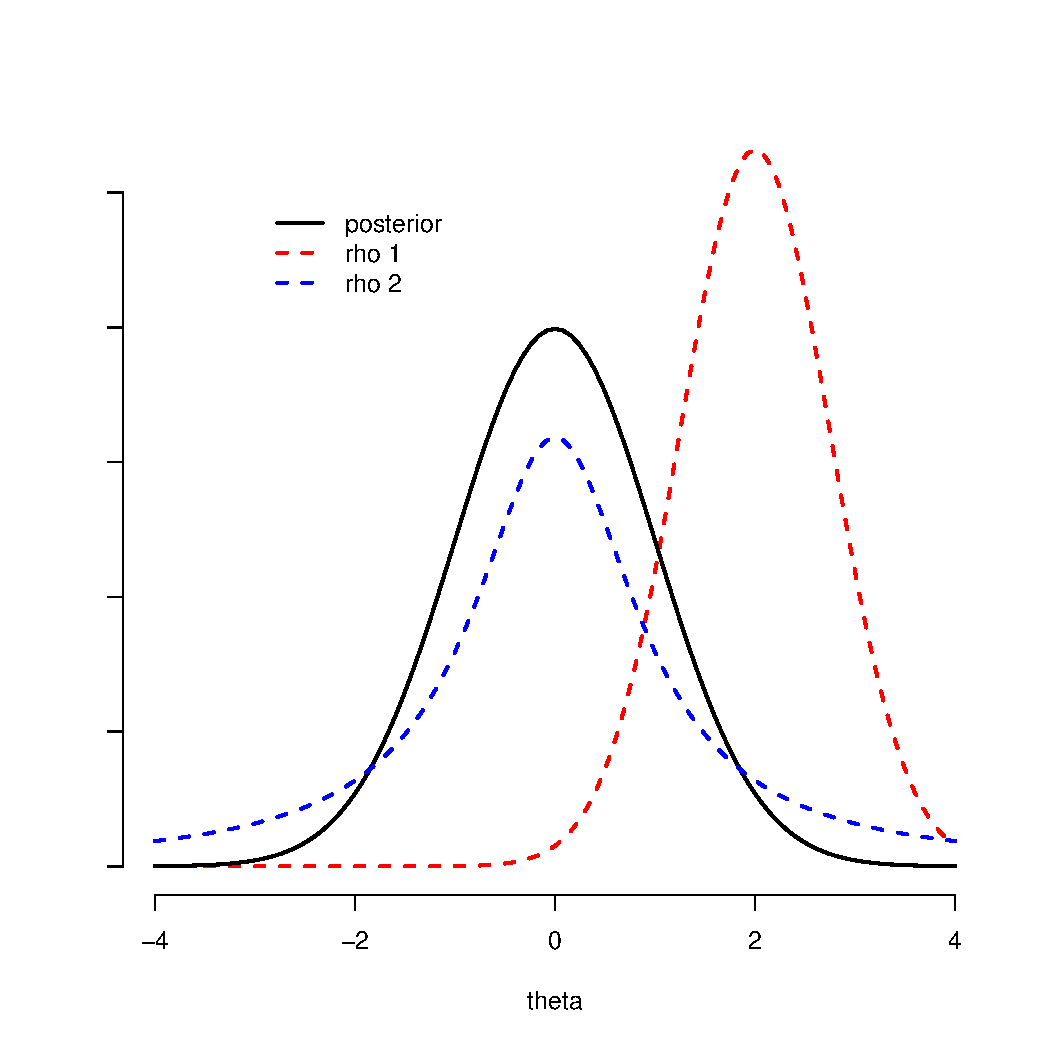
\includegraphics[scale=0.5]{figures/calcul/instrumentale.pdf}
\end{center}
\item Lorsque $\dim\Theta$ est petite (1 ou 2), on peut tracer $\pi(\theta|{\bf x_n})$ à un coefficient près pour sélectionner une forme intéressante pour $\rho(\theta)$.
\end{enumerate}
Un candidat logique peut parfois être la loi {\it a priori} $\pi(\theta)$, car elle respecte automatiquement la règle d'inclusion du support. Si l'{\it a priori} est très informatif par rapport aux données, l'{\it a posteriori} en sera proche. Une quantification de cette ``force" relative d'information est donc pratique pour choisir $\rho(\theta)$. Toutefois, ce choix peut être délicat : si l'{\it a priori} est très large (peu informatif), alors 
\begin{itemize}
\item il peut privilégier indûment des régions où la vraisemblance (comme fonction de $\theta$) est nulle ou quasi-nulle ;
\item  il faudra beaucoup de tirages pour atteindre les régions HPD (de plus haute densité) {\it a posteriori},  ce qui entraînera un  {coût algorithmique très fort}
\end{itemize}
Ce choix est aussi à proscrire si l'{\it a priori} privilégie des régions de $\Theta$ qui sont éloignées de celles privilégiées par les données. Une indication en faible dimension est de mesurer l'éloignement du mode {\it a priori} de $\theta$ et du maximum de vraisemblance $\hat{\theta}_n$. \\

\subsection{Méthodes d'échantillonnage dans la loi {\it a posteriori}}

Dans cette partie, on cherche doncà obtenir {\bf indirectement} des tirages qui suivent (en général approximativement) 
la loi {\it a posteriori}. Citons quelques algorithmes classiques que nous étudierons (quasiment tous) dans ce cours :
\begin{enumerate}
\item  algorithmes d'acceptation-rejet ;
\item  échantillonnage d'importance (préférentiel) ; 
\item  méthodes de Monte Carlo par chaînes de Markov (MCMC) ; 
\item  filtrage particulaire (pour les modèles à espace d'état).
\end{enumerate}
Ces méthodes  -- et leurs hybrides  -- sont les outils actuels les plus puissants pour simuler des lois connues semi-explicitement (à une constante/une intégrale près). Ils connaissent plusieurs approches d'\textbf{accélération} dont nous discuterons également, et qui amènent par ailleurs à faire un lien avec les techniques classiques du \emph{machine learning} : une technique de gradient stochastique, qui vise à estimer un mode {\it a posteriori} (et sous-entend en général que la loi {\it a posteriori} est approximativement gaussienne), peut être vue comme une forme dégénérée de MCMC adaptivement accélérée. \\

\subsubsection{Rappel : approches par inversion et transformations simples}

Rappelons avant de commencer que la méthode générique de simulation de $\theta\sim \pi(\theta|X)$ repose sur \emph{l'inversion de la fonction de distribution $\Pi$} qui, en unidimensionnel, est la fonction de répartition. \\

\begin{theorem}
Si $U\sim{\cal{U}}[0,1]$ et $\Pi(\theta|X)$ la fonction de répartition de $\theta|X$, alors $\Pi^{-1}(U|X)$ a la même loi que $\theta$.
\end{theorem}

La preuve vient du fait que par définition, $\Pi(\Pi^{-1}(U|X)\leq \theta|X)=\Pi(I\leq \Pi(\theta|X)|X)=\Pi(\theta|X)$. Si $\Pi$ n'est pas parfaitement croissante, on prend $\Pi^{-1}(u|X)=\inf\{\theta \ ; \ \Pi(\theta|X)\geq u\}$. \\



\begin{exo}
\begin{itemize} 
\item Loi binomiale ${\mathcal B}(n,p)$ : 
$
  F_X(x) = \sum_{i\le x} {n\choose i} p^i (1-p)^{n-i}
$
et $F_X^{-1}(u)$ s'obtient num\'eriquement.
\item  Loi exponentielle ${\mathcal E} (\lambda)$ :  
$
F_X(x) = 1 - \exp(\lambda x)$ et $
F_X^{-1}(u) = -\log({\textcolor{black}{\mathbf{u}}})/\lambda.
$
\item Loi de Cauchy ${\mathcal C} (0,1)$ : 
$
F_X(x) = \frac{1}{\pi} \arctan (x) + \frac{1}{2}$ et 
$ F_X^{-1}(u) = \tan(\pi({\textcolor{black}{\mathbf{u}}}-1/2))$. \\
.
\end{itemize}
\end{exo}

La critique de cette approche est aisée : $\Pi^{-1}(.|X)$ est rarement disponible, et ce ``théorème" (plutôt un lemme) d'inversion ne s'applique qu'en dimension 1. Pour "contrer" ces problèmes, on peut proposer quelques transformations (voir ci-dessous), mais cela ne permet de régler que des cas particuliers. \\

\begin{definition}{\bf Transformation de Box-M\"uller}
Pour la loi normale ${\mathcal N}(0,1)$, si $X_1,X_2\overset{iid}{\sim}{\mathcal N}(0,1)$, alors
$$
  X_1^2+X_2^2 \sim \chi^2_2, \qquad \arctan(X_1/X_2) \sim \mathcal{U}([0,2\pi]).
$$
%\rightline{\textcolor{black}{\sf[Jacobien]}}
Comme $\chi^2_2$ est identique \`a ${\mathcal E} (1/2)$, il vient par inversion :
$$
  X_1 = \sqrt{-2\,\log(U_1)} \,\sin (2\pi U_2)\qquad X_2 = \sqrt{-2\,\log(U_1)} \,\cos(2\pi U_2).
$$. 
\end{definition}

\noindent Les lois de Student et de Fisher se d\'eduisent naturellement
de la loi normale et de la loi du chi-deux. La loi de Cauchy se d\'eduit de la loi normale par la règle suivante : 
si $X_1,X_2\iid{\mathcal N}(0,1)$, alors $X_1/X_2 \sim {\mathcal C}(0,1)$. La loi Beta ${\mathcal B}_e(\alpha,\beta)$, de densit\'e
$$
  f_X(x) = \frac{\Gamma(\alpha+\beta)}{\Gamma(\alpha)\Gamma(\beta)}\,
	   x^{\alpha-1}(1-x)^{\beta-1}\,,
$$
s'obtient \`a partir de la loi gamma par la règle suivante : si 
$ X_1\sim {\mathcal G} a(\alpha,1)$, $X_2\sim {\mathcal G} a(\beta,1)$, alors
$$
  \frac{X_1}{X_1+X_2} \sim {\mathcal B}_e(\alpha,\beta). 
$$


\subsubsection{Simulation multidimensionnelle}\label{multidim.sim}

Le cas de la simulation multidimensionnelle est réglé également en principe par la règle en cascade suivante :

\begin{definition}{\bf Cascade rule.}
Supposons vouloir g\'en\'erer dans $\mathbb{R}^p$ l'échantillon 
$
(X_1,\ldots,X_p) \sim f(x_1,\ldots,x_p)
$
dont les composantes ne sont pas n\'ecessairement ind\'ependantes. La densité jointe s'écrit alors
$$
f(x_1,\ldots,x_p) = f_1(x_1)\times f_{2|1}(x_2|x_1)\ldots
\times f_{p|-p}(x_p|x_1,\ldots,x_{p-1}).
$$
On peut donc en déduire la règle d'implémentation suivante : \\

%{\makebox[0.5\textwidth][c]{\parbox{0.95\textwidth}{
\texttt{
Simuler pour $t=1,\ldots,T$
\begin{enumerate}
\item[1] {$X_1\sim f_1(x_1)$}
\item[2] {$X_2\sim f_{2|1}(x_2|x_1)$}
\item[ ] {$\vdots$}
\item[] {$X_p\sim f_{p|-p}(x_p|x_1,\ldots,x_{p-1})$}
\end{enumerate}
}
\end{definition}


\clearpage
\subsubsection{Algorithmes d'acception-rejet (AR)}

Ce type d'algorithme permet de simuler de façon {\bf exacte} et {\bf indépendante} selon la loi {\it a posteriori}. Il repose sur l'hypothèse suivante sur $\rho(\theta)$ :
$$
{\displaystyle 0 \ \ < \ \ K \ = \ \sup\limits_{\theta\in\Theta} \frac{f({\bf x_n}|\theta)\pi(\theta)}{\rho(\theta)} \ \ < \ \  \infty}.
$$

%\rule[0.5ex]{0.7\textwidth}{0.1mm} \\
 { \bf Algorithme AR:} \\
\rule[0.5ex]{0.7\textwidth}{0.1mm}
\vspace{-0.2cm}
\texttt{
\begin{enumerate}
\item { simulation indirecte :}  soit $\theta_i\sim \rho(\cdot)$ 
\vspace{0.05cm}
\item { test :} 
\begin{itemize} 
\item  soit $U_i\sim {\cal{U}}[0,1]$
\vspace{0.15cm}
\item  si ${\displaystyle U_i\leq \frac{f({\bf x_n}|\theta_i)\pi(\theta_i)}{K \rho(\theta_i)}}$ alors $\theta_i$ suit la loi $\pi(\theta|{\bf x_n})$
\end{itemize}
\end{enumerate}
\rule[0.5ex]{0.7\textwidth}{0.1mm}
}

\if\mycmdprooftwo1 \vspace{1cm} \begin{proof}%[Preuve] % Acceptation-rejet
Soit ${\theta}$ la variable aléatoire dont les tirages sont acceptées par le test. Alors, en définissant $P$ la mesure de probabilité usuelle sur $[0,1]$, et $\tilde{\Pi}$ la mesure de probabilité produit sur $\Theta\times[0,1]$, d'après la formule de Bayes,
\begin{eqnarray*}
\Pi\left(\tilde{\theta}\leq y | U \leq \frac{f({\bf x_n}|\theta)\pi(\theta)}{K\rho(\theta)} \right) & = & \frac{\tilde{\Pi}\left(\tilde{\theta}\leq y \ , \ U \leq \frac{f({\bf x_n}|\theta)\pi(\theta)}{K\rho(\theta)}\right)}{\tilde{\Pi}\left(U \leq \frac{f({\bf x_n}|\theta)\pi(\theta)}{K\rho(\theta)}\right)}, \\
& = & \frac{\int_{-\infty}^y \int_0^1 \frac{f({\bf x_n}|\theta)\pi(\theta)}{K\rho(\theta)} \ du \rho(\theta) \ d\theta}{\int_{-\infty}^{\infty} \int_0^{\frac{f({\bf x_n}|\theta)\pi(\theta)}{K\rho(\theta)}} \ du \rho(\theta) \ d\theta}, \\
& = & \frac{\int_{-\infty}^y f({\bf x_n}|\theta)\pi(\theta) \ d\theta}{K\int_{-\infty}^{\infty} \frac{1}{K}f({\bf x_n}|\theta)\pi(\theta) \ d\theta}, \\
& = & \Pi(\theta\leq y|{\bf x_n}).
\end{eqnarray*}
\end{proof}


\fi
\if\mycmdprooftwo0 {\it (Preuve en cours)}
\fi
\vspace{1cm}

Observons que la loi du nombre de tirages nécessaires selon $\rho(\theta)$ jusqu'à en accepter un suit la loi géométrique de probabilité $1/(K\cdot C)$ où $C$ est la constante d'intégration inconnue
\begin{eqnarray*}
C & = & \int_{\Theta} f({\bf x_n}|\theta)\pi(\theta) \ d\theta
\end{eqnarray*}
donc $K\cdot C$ est l'espérance du nombre de tirages nécessaires avant l'acceptation. \emph{Optimiser l'algorithme} revient donc à \emph{diminuer $K$}. 

\begin{exec}\label{quasi.conjug}
 On suppose $X   \sim {\cal{N}}(\theta,1)$ et on suppose connaître un échantillon ${\bf x_n}$ composé de :
\begin{itemize}
\item quelques observations $x_1,\ldots,x_{n-1}$ supposées iid. 
\item une pseudo-observation $y$ qui est un cas-limite masquant ({\it censurant}) une observation $x_{n}$ qui aurait dû être faite: $y<x_{n}$
\end{itemize}
 {\it A priori}, on suppose $\theta \sim {\cal{N}}(\mu,1)$. 
Pouvez-vous produire un algorithme d'AR qui génère des réalisations de la loi {\it a posteriori} de $\theta$ ? 
\end{exec}

\if\mycmdexotwo1 \vspace{1cm} \begin{rep}% AR
La vraisemblance s'écrit  
\begin{eqnarray*}
f({\bf x_n}|\theta) & \propto & \underbrace{\exp\left(-\frac{1}{2}\sum\limits_{k=1}^{n-1} (x_k-\theta)^2\right)}_{\text{\tiny terme régulier}} \ \ \ \left(\underbrace{1-\Phi(y-\theta)}_{\text{\tiny \begin{tabular}{l} terme dû à la censure \\ $\ \ = \ P(X>y)$ \end{tabular}}}\right).  
\end{eqnarray*}
L'{\it a posteriori} sur $\theta$ s'écrit alors
\begin{eqnarray*}
\pi(\theta|{\bf x_n}) & \propto & \tilde{\pi}(\theta|{\bf x_n}) \ = \ \exp\left\{-\frac{n}{2}\left[\theta - \frac{1}{n}\left(\mu + \sum\limits_{k=1}^{n-1} x_k\right)\right]^2\right\}\left\{1-\Phi(y-\theta)\right\}. 
\end{eqnarray*}
On remarque que si $y=x_n$, on aurait un modèle conjugué et $\pi(\theta|{\bf x_n})$ serait une loi normale. Il semble donc pertinent de proposer, comme choix de loi instrumentale,
$$
\rho(\theta) \equiv {\cal{N}}\left(\frac{1}{n}\left(\mu + \sum\limits_{k=1}^{n-1} x_k\right),1/n\right).
$$
Puisque $1-\Phi(y-\theta)\leq 1$, on a
\begin{eqnarray*}
\tilde{\pi}(\theta|{\bf x_n}) & \leq & \underbrace{\sqrt{\frac{2\pi}{n}}}_{K} \cdot\{1-\Phi(y-\theta)\}\cdot\rho(\theta).
\end{eqnarray*}
On peut donc mettre en oeuvre l'algorithme comme suit : on accepte $\theta_i$ si $U_i\leq 1-\Phi(y-\theta_i)$. Le nombre moyen d'appels nécessaires à $\rho(\theta)$ varie proportionnellement à $1/\sqrt{n}$, donc
plus l'échantillon de données grandit, plus l'algorithme est efficace.
Si cependant, on fait le choix $\rho(\theta)=\pi(\theta)$, alors
\begin{eqnarray*}
K & = & \sqrt{2\pi}\exp\left(\frac{1}{2}\left[\frac{1}{n-1}\sum\limits_{k=1}^n x_k - \mu\right](1-\sqrt{n})\right) 
\end{eqnarray*}
Voir la figure \ref{ARillus} pour une illustration de la mise en oeuvre de cet algorithme.
\end{rep}

\begin{figure}[hbtp]
\begin{center}
\includegraphics[scale=0.3]{figures/calcul/AR1.png} \\
\includegraphics[scale=0.3]{figures/calcul/AR2.png}
\caption{
Essai de simulation par AR en utilisant (en haut) une loi instrumentale ``proche" du vrai posterior ; (en bas) le prior comme loi instrumentale.}
\label{ARillus}
\end{center}
\end{figure}

\fi

\clearpage
\begin{exec}\label{gamma}
Soit un échantillon de loi gamma $x_1,\ldots,x_n\overset{iid}{\sim} {\cal{G}}(a,\theta)$ où $a$ est connu. On suppose $\pi(\theta)\equiv {\cal{G}}(c,d)$. Produisez une méthode par AR pour simuler la loi {\it a posteriori} $\pi(\theta|x_1,\ldot,x_n)$ et vérifiez que les tirages obtenus sont bien issus de cette loi, par ailleurs explicite.
\end{exec}

\if\mycmdexotwo1 \vspace{1cm} \begin{rep}
Il est aisé de vérifier qu'on connaît parfaitement la loi {\it a posteriori} de $\theta$ :
\begin{eqnarray*}
\theta|x_1,\ldots,x_n %& \sim & \pi(\theta|x_1,\ldots,x_n) \ \propto \ \\
& \sim & {\cal{G}}\left(c+an,d+\sum\limits_{i=1}^n x_i\right).
\end{eqnarray*}
On peut donc vérifier l'accord entre un échantillon iid simulé par AR et cette loi, via des tests statistiques classiques comme Kolmogorov-Smirnov, Cramer-von Mises ou Anderson-Darling. Pour construire cet algorithme d'AR, faisons par exemple le choix d'une loi instrumentale lognormale (qui est bien à support positif, car $\theta>0$) :
\begin{eqnarray*}
\rho(\theta|\mu,\sigma) & = & \frac{1}{\theta\sigma \sqrt{2\pi}} \exp\left(-\frac{1}{2\sigma^2}\left(\mu-\log\theta\right)^2\right).
\end{eqnarray*}
Il vient alors 
\begin{eqnarray*}
\kappa(\theta|\mu,\sigma)  \ = \  \frac{f(x_1,\ldots,x_n|\theta)\pi(\theta)}{\rho(\theta)} & = & {\displaystyle \frac{\sqrt{2\pi} \sigma \theta^{c+an} \exp\left(-\theta(d+\sum_{i=1}^n x_i)\right)}{\exp\left(-\frac{1}{2\sigma^2}\left(\mu-\log\theta\right)^2\right)}}
\end{eqnarray*}
et 
\begin{eqnarray*}
\frac{\partial }{\partial \theta} \log \kappa(\theta|\mu,\sigma) & = & \frac{c+an}{\theta} - \left(d+\sum\limits_{i=1}^n x_i\right) - \frac{1}{\sigma^2\theta}\left(\mu-\log(\theta)\right), \\
\frac{\partial^2 }{\partial \theta^2} \log \kappa(\theta|\mu,\sigma) & = & \frac{1}{\theta^2}\left(-(c+an) + \frac{1}{\sigma^2}(1+\mu - \log(\theta)\right).
\end{eqnarray*}
Notons $\theta_0(\mu,\sigma)=\exp(-(c+an)+(1+\mu)/\sigma^2)$. Si $0\leq \theta\leq \theta_0$, alors $\frac{\partial }{\partial \theta} \log \kappa(\theta|\mu,\sigma)$ est croissante. Si $\theta>\theta_0$, elle est décroissante vers $-(d+\sum_{i=1}^n x_i)<0$. Pour permettre à $\kappa(\theta|\mu,\sigma)$ d'être maximisable sur $\theta>0$, il faut donc que 
$$
\frac{\partial }{\partial \theta} \log \kappa(\theta_0(\mu,\sigma)|\mu,\sigma) = -\left(d+\sum\limits_{i=1}^n x_i\right) + 1/\sigma^2\theta_0 \ > \ 0.
$$
Sous cette contrainte, on peut résoudre numériquement en $\theta=\theta_1(\mu,\sigma)>\theta_0(\mu,\sigma)$ l'équation $\frac{\partial }{\partial \theta} \log \kappa(\theta|\mu,\sigma)=0$, et $\theta_1(\mu,\sigma)$ maximise alors $\kappa(\theta|\mu,\sigma)$. Dans ce cas, on peut définir 
\begin{eqnarray*}
K & = & \arg\min\limits_{\mu,\sigma} \kappa(\theta_1(\mu,\sigma)|\mu,\sigma). 
\end{eqnarray*}
et mettre en place l'algorithme AR.
\end{rep}
\fi

\begin{remark} On peut améliorer (faire baisser) le taux de rejet en encadrant la loi {\it a posteriori} entre 2 densités instrumentales 
 ({ acceptation-rejet par {\it enveloppe}}). \\
 \end{remark}
 
Le principe de l'AR est parfait en théorie, mais en pratique il est réservé aux cas simples ($\dim\Theta$ petite). De plus, cet algorithme est en général très coûteux en temps d'attente. 


\subsubsection{Algorithmes d'échantillonnage préférentiel ou d'importance (IS)}

Ce type d'algorithme vise surtout à produire un estimateur consistant d'une quantité d'intérêt {\it a posteriori}, mais il peut être utilisé dans un but de produire un échantillonnage exact mais non indépendant de la loi-cible (approche SIR). \\

{\bf Algorithme IS:} \\
\rule[0.5ex]{0.8\textwidth}{0.1mm}
\vspace{-0.2cm}
\texttt{
\begin{enumerate}
\item Soit $(\theta_1,\ldots,\theta_M)$ un tirage i.i.d. selon une densité instrumentale $\rho(\theta)$.
\item Soit $(\omega_1,\ldots,\omega_M)$ les {\bf poids d'importance} définis par
\begin{eqnarray*}
\omega_i & \propto &  \frac{f({\bf x_n}|\theta_i)\pi(\theta_i)}{\rho(\theta_i)}
\end{eqnarray*}
et normalisés de façon à ce que leur somme fasse 1.
\end{enumerate}
\rule[0.5ex]{0.8\textwidth}{0.1mm}
}

\begin{theorem}{Geweke 1989.}
Toute fonction {\it prédictive}
\begin{eqnarray*}
h(x|{\bf x_n}) & = & \int_{\Theta} h(x|\theta) \pi(\theta|{\bf x_n}) \ d\theta
\end{eqnarray*}
(ex: $h=f$) peut être estimée de façon consistante, lorsque $M\rightarrow\infty$, par
\begin{eqnarray*}
\hat{h}(x|{\bf x_n}) & = & \sum\limits_{i=1}^M \omega_i h(x|\theta_i).
\end{eqnarray*}
\end{theorem}

L'approche {\it Sampling-Importance Resampling} (SIR), proposée par Rubin (1988), se fonde sur le résultat suivant : 

\begin{theorem}\label{SIR.rubin}
Les tirages
\begin{eqnarray*}
\tilde{\theta}_1,\ldots,\tilde{\theta}_P & \sim & {\cal{M}}_{ultinomial}\left(\theta_1,\ldots,\theta_M|\omega_1,\ldots,\omega_M\right)
\end{eqnarray*}
suivent la loi {\it a posteriori} $\pi(\theta|{\bf x_n})$.
\end{theorem}

L'heuristique de Rubin consiste à prendre $P<M/20$ pour diminuer la dépendance dans l'échantillon resimulé. On peut aussi ainsi estimer les caractéristiques de $\pi(\theta|{\bf x_n})$ (moyenne, variance, etc.). \\

\begin{exo}
En reprenant une solution proposée pour l'exemple \ref{quasi.conjug}, par exemple $\rho(\theta) \equiv {\cal{N}}(\mu + \sum_{k=1}^{n-1} x_i,1/n)$, les poids sont simplement proportionnels à 
\begin{eqnarray*}
\omega_i & \propto & 1-\Phi(y-\theta_i)  
\end{eqnarray*}
qu'on normalise en divisant le membre de droite par la somme des $1-\Phi(y-\theta_i)$, $i=1,\ldots,M$. Les poids les plus hauts sont donc ceux pour lesquels $y \ll \theta_i$. \\
\end{exo}

Remarquons que fort logiquement, plus la densité instrumentale $\rho(\theta)$ est ``proche" de $\pi(\theta|{\bf x_n})$, plus les poids sont équilibrés (donc meilleur est le rééchantillonnage). Voir figure \ref{resume-IS} pour un résumé. Plutôt qu'une loi unique $\rho$, on peut mettre en place des algorithmes {\it adaptatifs} qui construisent itérativement une suite de densités $\{\rho_k(\theta)\}_k$ convergeant vers $\pi(\theta|{\bf x_n})$, pour améliorer encore le rééchantillonage. Une revue de tels algorithmes est proposée dans \cite{Marin2007}.   \\

\begin{figure}[h!]
\centering
\includegraphics[scale=0.3]{figures/calcul/is.png}
\caption{Schématisation du principe de l'échantillonnage d'importance.}
\label{resume-IS}
\end{figure}

Notons le résultat suivant, important et dû à Rubinstein (1981), qui guide ces recherches d'algorithmes IS optimaux. Ce résultat n'est pas exploitable directement, car il revient à avoir déjà résolu que l'on cherche à résoudre, mais il sert à construire des lois instrumentales qui progressivement vont se rapprocher de cette optimalité. 

\begin{theorem}{Importance sampling optimal.}
Soit l'estimateur de la fonction d'intérêt $h(\theta)\in\R$ par IS :
\begin{eqnarray*}
\hat{h}_M & = & \frac{1}{M}\sum\limits_{i=1}^M \frac{\pi(\theta_i|x)}{\rho(\theta_i)} h(\theta_i) \ \to \ \E_{\pi}[h(\theta|X] \ \ \ p.s.
\end{eqnarray*}
où les $\theta_i\overset{iid}{\sim} \rho(\theta)$. Alors le choix de $\rho$ qui minimise la variance de l'estimateur $\hat{h}_M$ est 
\begin{eqnarray*}
\rho^*(\theta) & = & \frac{|h(\theta)|\pi(\theta|X)}{\int_{\Theta}|h(\theta)|\pi(\theta|X) \ d\theta}.
\end{eqnarray*}
\end{theorem}

\if\mycmdprooftwo1 \vspace{1cm} \begin{proof}%[Preuve] % IS optimal
On note d'abord que
\begin{eqnarray*}
\V_{\rho}\left[\frac{h(\theta)\pi(\theta|x)}{\rho(\theta)}\right] & = & \E_{\rho}\left[\frac{h^2(\theta)\pi^2(\theta|x)}{\rho^2(\theta)}\right]-  \left(\E_{\rho}\left[\frac{h(\theta)\pi(\theta|x)}{\rho(\theta)}\right]\right)^2
\end{eqnarray*}
et que le second terme ne dépend pas de $\rho$. Il suffit donc de minimiser le premier terme. D'après l'inégalité de Jensen,  on a donc,
\begin{eqnarray*}
\E_{\rho}\left[\frac{h^2(\theta)\pi^2(\theta|x)}{\rho^2(\theta)}\right] & \geq & \left(\E_{\rho}\left[\frac{|h(\theta)|\pi(\theta|x)}{\rho(\theta)}\right]\right)^2, \\
& \geq & \left(\int_{\Theta} |h(\theta)|\pi(\theta|x) \ d\theta\right)^2
\end{eqnarray*}
qui est une borne inférieure indépendante de $\rho$, qui est atteinte en $\rho^*$.
\end{proof}
\fi
\if\mycmdprooftwo0 {\it (Preuve en cours)}
\fi
\vspace{1cm}



Un outil important, dès qu'on aborde le problème de la génération de données de même loi, mais corrélées, est la {\bf taille d'échantillon effective}, notée en général ESS (\emph{Effective Sample Size}). L'ESS relie la variance d'un estimateur de Monte Carlo idéal (échantillonnant directement dans la loi-cible) à la variance d'un estimateur fondé sur un échantillonnage corrélé, comme celui produit par l'IS, dans le cas où les deux estimateurs utilisent le même nombre de tirages. L'ESS mesure donc l'efficacité d'un algorithme d'échantillonnage corrélé. \\

\begin{definition}{\bf Effective Sample Size.}
Soit un échantillonnage instrumental $(\theta_1,\ldots,\theta_M)$ associé à des poids d'importance normalisés $(\omega_1,\ldots,\omega_M)$. Alors on définit
\begin{eqnarray*}
\mbox{ESS} & = & \left(\sum\limits_{i=1}^M \omega^2_i\right)^{-1}.
\end{eqnarray*}
\end{definition}

Lorsque l'échantillon produit est bien indépendant, les poids normalisés sont tous égaux à $1/M$, et donc $\mbox{ESS}=M^2/M=M$. \\

\begin{remark}
Dans le cas des MCMC, la définition précédente nécessite d'être remaniée pour tenir compte de la corrélation dans l'échantillonnage obtenu. \\
\end{remark}

Une autre propriété intéressante des techniques d'IS est de permettre de mener facilement certains types d'\textbf{analyse de sensibilité au prior}. Nous l'analysons dans l'exercice suivant.

\begin{exec}
Considérons une fonction d'intérêt $h(\theta)$ que l'on cherche à résumer par un estimateur calculé sous un coût quadratique ; il s'agit donc de l'espérance {\it a posteriori}
\begin{eqnarray}
h \ = \ \E_{\pi}[h(\theta)|x_1,\ldots,x_n] & = & \int_{\Theta} h(\theta)\pi(\theta|x_1,\ldots,x_n) \ d\theta\label{IS.estim1}
\end{eqnarray}
que l'on suppose pouvoir estimer simplement, de fa\c con consistante, par Monte Carlo. Supposons vouloir modifier le prior : $\pi(\theta)\to\pi'(\theta)$, sans modifier le support, mais de fa\c con à ce que la nouvelle loi {\it a posteriori} ne soit plus directement simulable. Peut-on (et sous quelles conditions) ne pas faire de calcul supplémentaire pour simuler le nouveau posterior $\pi'(\theta\x_1,\ldots,x_n)$ ?
\end{exec}

\if\mycmdexotwo1 \vspace{1cm} \begin{rep}
On considére donc une fonction d'intérêt $h(\theta)$ que l'on cherche à résumer par son espérance {\it a posteriori}
\begin{eqnarray}
h \ = \ \E_{\pi}[h(\theta)|x_1,\ldots,x_n] & = & \int_{\Theta} h(\theta)\pi(\theta|x_1,\ldots,x_n) \ d\theta\label{IS.estim1}
\end{eqnarray}
que l'on suppose pouvoir estimer simplement, de fa\c con consistante, par Monte Carlo :
\begin{eqnarray*}
\hat{h}_M & = & \frac{1}{M}\sum\limits_{k=1}^M h(\theta_i) \ \ \ \text{avec $\theta_i\overset{iid}{\sim} \pi(\theta|x_1,\ldots,x_n)$}
\end{eqnarray*}
Supposons vouloir modifier le prior : $\pi(\theta)\to\pi'(\theta)$, sans modifier le support, mais de fa\c con à ce que la nouvelle loi {\it a posteriori} ne soit plus directement simulable. En supposant que $\pi(\theta|x_1,\ldots,x_n)>0$ pour tout $\theta\in\Theta$, on peut néanmoins recalculer facilement le nouvel estimateur de Bayes :
\begin{eqnarray*}
h' \ = \ \E_{\pi'}[h(\theta)|x_1,\ldots,x_n] & = & \int_{\Theta} h(\theta)\pi'(\theta|x_1,\ldots,x_n) \ d\theta, \\
& = & \int_{\Theta} \omega(\theta_i) h(\theta)\pi(\theta|x_1,\ldots,x_n) \ d\theta
\end{eqnarray*}
avec
\begin{eqnarray*}
\omega(\theta_i) & = & \frac{\pi'(\theta|x_1,\ldots,x_n) }{\pi(\theta|x_1,\ldots,x_n)} \ = \ C\tilde{\omega}^*_i 
\end{eqnarray*}
où 
\begin{eqnarray*}
\tilde{\omega}^*_i  & = & \left(\frac{\pi'(\theta_i)}{\pi(\theta_i)}\right), \\
C & = &  \frac{m_{\pi}(x_1,\ldots,x_n)}{m_{\pi'}(x_1,\ldots,x_n)}.
\end{eqnarray*}
Le calcul de la constante de proportionnalité $C$ nécessiterait usuellement de disposer de deux échantillons {\it a posteriori}. On peut cependant s'en passer en remarquant que d'après la loi forte des grands nombres,  \begin{eqnarray*}
\frac{1}{M}\sum\limits_{i=1}^M \tilde{\omega}^*_i & \xrightarrow[n\to \infty]{p.s.} & \frac{1}{C}\int_{\Theta} \omega(\theta) \pi(\theta|x_1,\ldots,x_n) \ d\theta \ = \ 1/C
\end{eqnarray*}
et on en déduit donc qu'un estimateur IS  consistant de $h'$,  qui réutilise les calculs faits pour l'estimateur $\hat{h}_M$  sans coût calculatoire additionnel, est 
\begin{eqnarray*}
\hat{h''}_M & = & \frac{1}{M}\sum\limits_{k=1}^M \hat{\omega}^*_i h(\theta_i)
\end{eqnarray*}
avec
\begin{eqnarray*}
\hat{\omega}^*_i & = & \frac{\tilde{\omega}^*_i}{\sum\limits_{j=1}^M \tilde{\omega}^*_j}.
\end{eqnarray*}

 %\left(\frac{\pi'(\theta)}{\pi(\theta)}\right) \left(\frac{m_{\pi}(x_1,\ldots,x_n)}{m_{\pi'}(x_1,\ldots,x_n)}\right)
%\end{eqnarray*}
%Le second terme entre parenthèses ne dépend pas de $\theta$. En faisant l'hypothèse suivante :
%\begin{eqnarray*}
%\forall i\in\{1,\ldots,M\}, \ \ \pi(\theta_i_>0, \label{prior.pos}
%\end{eqnarray*}
%on peut donc proposer l'estimateur IS suivant pour $h'$, qui réutilise les calculs faits pour l'estimateur $\hat{h}_M$ : 
%\begin{eqnarray*}
%\hat{h'}_M & = & \frac{1}{M}\sum\limits_{k=1}^M \tilde{\omega}_i h(\theta_i)
%\end{eqnarray*}
%avec
%\begin{eqnarray*}
%\tilde{\omega}_i  =  C\tilde{\omega}^*_i & \text{et} & 
%\tilde{\omega}^*_i  =  \left(\frac{\pi'(\theta_i)}{\pi(\theta_i)}\right),
%\end{eqnarray*}
%et $C$ la constante de proportionnalité 
%\begin{eqnarray*}
%C & = & \frac{m_{\pi}(x_1,\ldots,x_n)}{m_{\pi'}(x_1,\ldots,x_n)}
%\end{eqnarray*}
%dont le calcul nécessite en théorie uniquement des tirages des deux priors (par Monte Carlo). Cependant, on remarque que par la loi forte des grands nombres, que 
%\begin{eqnarray*}
%\frac{1}{M}\sum\limits_{i=1}^M \tilde{\omega}^*_i & \xrightarrow[n\to \infty]{p.s.} & 
%\end{eqnarray*}

%On remarque, par la loi forte des grands nombres,  que

%\E\left[\frac{1}{M}\sum\limits_{i=1}^M \tilde{\omega}^*_i\right] \ = \ \frac{1}{M}\sum\limits_{i=1}^M \int_{\Theta} \pi'(\theta) \ d\theta \ = \ 1.
%\end{eqnarray*}
%Cependant, on sait que le calcul par Monte Carlo selon des tirages {\it a priori} du rapport $C$ des lois marginales peut être fortement instable. Il est donc simplement conseillé d'adopter la démarche suivante, suivant le théorème \ref{SIR.rubin} :
%\begin{enumerate}
%\item calculer les poids relatifs $\tilde{\omega}^*_i$ ;
%\item resimuler avec remise dans $\theta_1,\ldots,\theta_M$ selon les poids $\tilde{\omega}^*_i$ pour obtenir de nouveaux tirages {\it a posteriori} de $\pi'(\theta|x_1,\ldots,x_n)$. 
%\end{enumerate}
Notons que ce faisant, on crée de la corrélation entre les deux estimateurs de $h$. 
\end{rep}
\fi









\subsubsection{Méthodes de Monte Carlo par Chaînes de Markov (MCMC)}\label{MCMC}

Le principe des MCMC est de partir d'un tirage d'une densité $\tilde{\pi}_0(\theta)$ arbitraire, puis de 
produire une \emph{chaîne de Markov} de réalisations $\theta^{(1)},\ldots,\theta^{(M)}$ qui a pour loi
{\bf stationnaire} $\pi(\theta|{\bf x_n})$. \\ %Rappelons une série  de termes et résultats importants pour la construction et l'usage des MCMC. \\

\begin{definition}{\bf Noyau de transition.}
Une chaîne de Markov homogène est déterminée par un \emph{noyau de transition}, défini sur $\Theta\times {\cal{B}}(\Theta)$ à l'itération $i$ par 
\begin{eqnarray*}
{\cal{K}}(\theta|A) & = & P(\theta^{(i)}\in A | \theta^{(i-1)}=\theta) \ = \ \int_{A} \underbrace{{\kappa}(\theta,\tilde{\theta})}_{\text{\tiny densité de transition sur $\tilde{\theta}$}} \ d\tilde{\theta},
\end{eqnarray*} 
telle que ${\cal{K}}(.|A)$ est mesurable $\forall A \in {\cal{B}}(\theta)$. Cette notion de noyau généralise au cadre continu celle de matrice de transition d'un état à un autre dans un cadre discret. 
\end{definition}

\noindent Toute la structure d'une chaîne de Markov, que l'on considèrera toujours d'ordre 1 dans ce cours, dépend seulement du choix d'un noyau de transition et de l'état initial (ou la distribution initiale) de la chaîne, comme l'exprime la définition suivante. 

\begin{definition}{\bf Chaîne de Markov.}
 Sachant un noyau de transition ${\cal{K}}$, une suite $\theta_0,\ldots,\theta_n,\ldots$ de variables aléatoires est une chaîne de Markov d'ordre 1 si, $\forall n\geq 0$, la distribution de $\theta_n$ conditionnelle à la $\sigma-$algèbre (filtration) générée par $\theta_{n-1},\theta_{n-2},\ldots,\theta_0$ est la même que celle de $\theta_{n}|\theta_{n-1}$ :
 \begin{eqnarray*}
 \pi\left(\theta_n\in {\cal{A}} | \theta_{n-1},\theta_{n-2},\ldots,\theta_0\right) & = & \pi\left(\theta_n\in {\cal{A}} | \theta_{n-1}\right), \ 
 = \  {\cal{K}}(\theta_{n-1}|{\cal{A}}).
 \end{eqnarray*}
\end{definition}

\noindent Des éléments fondamentaux de théorie des chaînes de Markov sont rappelés en Annexe \ref{markovtheory}. Nous en retenons surtout un résultat fondamental, le \emph{théorème ergodique}. Celui-ci nous donne "le droit", sous certaines conditions, de mener des calculs de Monte Carlo à partir de chaînes de valeurs corrélées produites par une chaîne de Markov. On parlera alors de méthode de Monte Carlo par chaîne de Markov (MCMC).  

\begin{theorem}{\bf (Théorème ergodique).}\label{theorem.ergogique}
Si la chaîne de Markov $(\theta_n)_{n\geq 0}$ est réccurente positive\footnote{Plus précisément Harris-récurrente positive, cf. Annexe \ref{markovtheory}.}, alors pour toute fonction $h:\Theta\to\R$ telle que $\E_{\pi}[|h| \ | x_1,\ldots,x_n] ]<\infty$, alors
$$
\lim\limits_{n\to\infty} \frac{1}{n} \sum\limits_{i=1}^n h(\theta_i)  =  \int_{\Theta} h(\theta) \ d\Pi(\theta|x_1,\ldots,x_n).
$$
Si de plus la chaîne $(\theta_n)_{n\geq 0}$ est réversible, alors 
\begin{eqnarray*}
\frac{1}{\sqrt{n}} \sum\limits_{i=1}^n \left(h(\theta_i)-\E_{\pi}[h  | x_1,\ldots,x_n] \right) & \xrightarrow[n\to\infty]{{\cal{L}}} & {\cal{N}}(0,\gamma^2)
\end{eqnarray*}
avec
$$
0 \ < \ \gamma^2 = \E_{\pi}\left[h^2(\theta_0)  | x_1,\ldots,x_n\right] + 2 \sum\limits_{k=1}^{\infty} \E_{\pi}\left[h(\theta_0) h(\theta_k)  | x_1,\ldots,x_n\right] \ < \ \infty.
$$
\end{theorem}


\paragraph{Caractéristiques générales d'une MCMC.}
\`A l'itération $i$ d'une MCMC, la densité de probabilité d'un $\theta$ simulé est
$$
\tilde{\pi}_i(\theta)  =  \int_{\hat{\theta}\in\Theta} \tilde{\pi}_{i-1}(\hat{\theta}) {\kappa}(\hat{\theta},\theta) \ d\hat{\theta}
$$
et converge en loi vers une \emph{unique densité stationnaire $\tilde{\pi}_{\infty}(\theta)$}, indépendamment de $\tilde{\pi}_0$, sous des conditions très générales de convergence et d'unicité :
\begin{itemize}
\item tout état (ou sous-ensemble) de $\Theta$ est accessible à partir de n'importe quel autre état  ({\it irréductibilité}) ;
\item le nombre minimal d'états intermédiaires est nul  ({\it apériodicité}) ; cela se traduit, lorsque $\Theta$ est discret, par le fait que la chaîne ne peut pas boucler sur un ensemble d'états ; 
\item l'espérance du temps de retour en n'importe quel état est fini ({\it récurrence positive}).
\end{itemize}
Les caractéristiques majeures d'une MCMC sont les suivantes (cf. figure \ref{ex-mcmc-1}) :
\begin{itemize}
\item le début de la chaîne (dit \emph{\it temps de chauffe}) sert à explorer l'espace $\Theta$ et trouver les zones de {\bf haute densité {\it a posteriori}} ;
\item on ne conserve que la seconde partie de l'ensemble des $\theta^{(i)}$ produits, qui suivent la distribution stationnaire (la chaîne ``oublie" son état initial) ; 
\item la fréquence de visite de chaque état (ou sous-ensemble) de $\Theta$ est la même pour toute trajectoire MCMC ; 
\item on ajoute souvent une étape de \emph{rééchantillonage} (SIR) ou de \emph{décorrélation} des $\theta^{(i)}$ conservés pour obtenir
un échantillon approximativement indépendant de $\tilde{\pi}_{\infty}(\theta)$.  \\
\end{itemize} 





\paragraph{Application au bayésien.}
Si on veut appliquer le principe des MCMC au bayésien, il faut que la loi stationnaire $\tilde{\pi}_{\infty}(\theta)$ soit la loi {\it a posteriori} $\pi(\theta|{\bf x_n})$. Pour cela, le noyau ${\cal{K}}$ doit être construit en fonction de la vraisemblance des données ${\bf x_n}$ et de l'{\it a priori} $\pi(\theta)$. On peut prosa\"iquement réutiliser la structure de  l'algorithme d'Acceptation-Rejet, en créant un noyau résultant du mélange de deux actions à l'itération $i$ :
\begin{itemize}
\item on accepte un nouveau candidat-tirage de $\tilde{\pi}_i(\theta)$ avec une probabilité $\alpha_i$ ;
\item on refuse et on conserve le tirage précédent dans la chaîne avec probabilité $1-\alpha_i$.
\end{itemize}
Ce type d'algorithme a été formalisé et est connu sous le nom d'\textbf{algorithme de Hastings-Metropolis} (HM). Sous certaines conditions de conditionnement explicite {\it a posteriori}, on peut accepter des candidats avec probabilité $1$. Ceci donne une forme particulière de MCMC, connue sous le nom d'\textbf{algorithme de Gibbs}. \\

\paragraph{Algorithme HM.} La structure de l'algorithme est la suivante. \\%Soit une densité instrumentale $\rho(\theta|\theta^{(i-1)})$.

\texttt{\'Etape $i$: \\
\rule[0.5ex]{0.8\textwidth}{0.1mm}
\vspace{-0.2cm}
\begin{enumerate}
\item Simuler selon une loi instrumentale $\tilde{\theta} \sim \rho(\theta|\theta^{(i-1)})$.
\item Calculer la probabilité 
\begin{eqnarray*}
\alpha_i & = & \min\left\{1,\left(\frac{f({\bf x_n}|\tilde{\theta})\pi(\tilde{\theta})}{f({\bf x_n}|{\theta^{(i-1)}})\pi({\theta^{(i-1)}})}\right)\cdot\left(\frac{\rho(\theta^{(i-1)}|\tilde{\theta})}{\rho(\tilde{\theta}|\theta^{(i-1)})}\right)\right\}.
\end{eqnarray*}
\item $\left.\begin{tabular}{l}
\text{Simuler $U\sim{\cal{U}}_{\text{\tiny unif}}[0,1]$}. \\
\\
\text{Si $U\leq \alpha_i$ choisir $\theta^{(i)}=\tilde{\theta}$}. \\
\text{Sinon choisir $\theta^{(i)}=\theta^{(i-1)}$}. 
\end{tabular}\right\}$ Accepter $\tilde{\theta}$ avec probabilité $\alpha_i$. 
\end{enumerate}
\rule[0.5ex]{0.8\textwidth}{0.1mm}
}

\vspace{0.5cm}

Le noyau markovien est alors constitué d'un mélange d'un Dirac en $\theta^{(i-1)}$ et de la loi instrumentale, mélange pondéré par la probabilité de transition $\alpha_i$. La partie continue
du noyau de transition (de $\theta$ vers $\theta'$) s'écrit
\begin{eqnarray*}
p(\theta,\theta')  & = & \alpha(\theta,\theta')\rho(\theta'|\theta)
\end{eqnarray*}
avec $\alpha(\theta,\theta')$ la probabilité de transition
\begin{eqnarray*}
\alpha(\theta,\theta') & = & \min\left\{1,\left(\frac{f({\bf x_n}|\theta')\pi(\theta')}{f({\bf x_n}|{\theta})\pi(\theta)}\right)\cdot\left(\frac{\rho(\theta|\theta')}{\rho(\theta'|\theta)}\right)\right\}.
\end{eqnarray*}
On a  
\begin{eqnarray*}
\pi(\theta) \times p(\theta,\theta')  & = & \pi(\theta') \times p(\theta',\theta).
\end{eqnarray*} 
La chaîne MCMC produite est alors dite \emph{réversible} et ceci suffit à montrer, si la chaîne est irréductible et  apériodique, que :
\begin{itemize}
\item elle est ergodique ; 
\item la distribution des itérés $\theta^{(i)},\ldots,\theta^{(j)}$ de la chaîne converge en loi vers une loi-limite unique ; 
\item celle-ci est proportionnelle à $f({\bf x_n}|\theta)\pi(\theta)$ : il s'agit donc de $\pi(\theta|{\bf x_n})$.
\end{itemize}
L'irréductibilité peut être facilement assurée par la contrainte suivante : le support de la loi instrumentale doit inclure le support de la loi-cible. \\

Le rapport de Metropolis fait intervenir le rapport des lois {\it a posteriori} (qui permet d'\^oter la constante d'int\' egration inconnue) : à l'étape $k$, si $\tilde{\theta}_{k}$ se situe plus haut dans la  zone de haute densit\' e de $\pi(\theta|{\bf x_n})$ que $\theta_{k-1}$, ce rapport est plus grand que 1. Le rapport inverse des lois instrumentales et l'usage d'un tirage uniforme interdisent d'automatiser l'acceptation de ce nouveau point, en permettant \`a la cha\^ine de Markov d'explorer exhaustivement l'espace $\Theta$. \\




\begin{exec}\label{debit.extreme}
Soit $X$ la variable ``débit maximal de rivière". Elle est supposée suivre une loi des extrêmes (Gumbel) de densité
\begin{eqnarray*}
f(x|\theta) & = &  \lambda\mu\exp(-\lambda x)
\exp(-\mu\exp(-\lambda x)).
\end{eqnarray*}
avec $\theta=(\mu,\lambda)$. %L'espérance est
%\begin{eqnarray*}
%\E[X|\theta] & = & \lambda^{-1}\left(\log \mu + \gamma\right)
%\end{eqnarray*}
%où $\gamma$ est la constante d'Euleur ($\simeq$ 0.578..)
\begin{center}
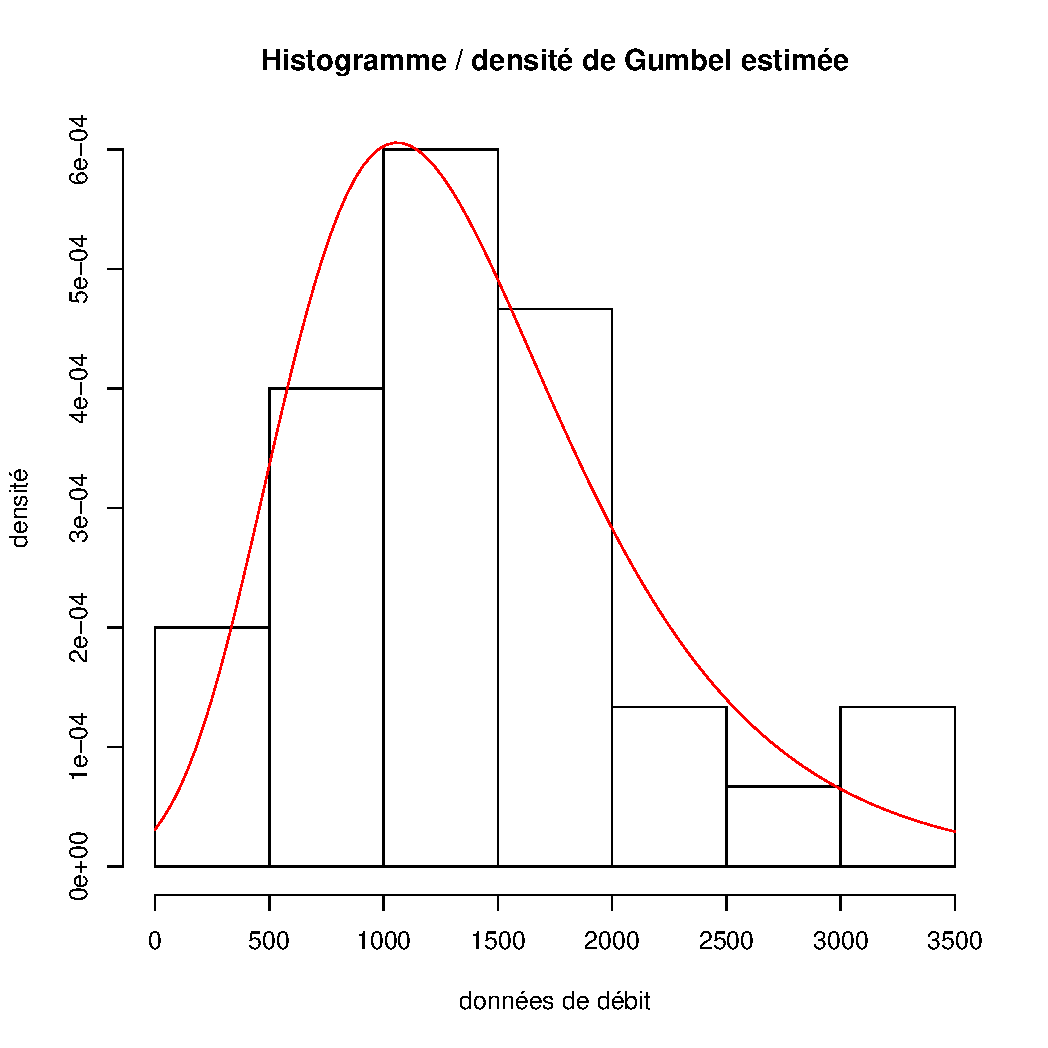
\includegraphics[scale=0.4]{figures/calcul/hist-gumbel.pdf}
\end{center}
Considérons $n$ observations ${\bf x_n}=(x_1,\ldots,x_n)$ supposées iid  selon cette distribution. 
\begin{enumerate}
    \item Comment s'écrit la vraisemblance ?
    \item On considère l'{\it a priori} $\pi(\mu,\lambda) = \pi(\mu|\lambda)\pi(\lambda)$ avec
\begin{eqnarray*}
\mu|\lambda & \sim   & {\cal{G}}\left(m,b_m(\lambda) \right),  \\
\lambda    & \sim   & {\cal{G}}\left(m,m/\lambda_e\right)
\end{eqnarray*}
et ${\displaystyle b_m(\lambda)  = \left[\alpha^{-1/m}
-1\right]^{-1} \exp(-\lambda x_{e,\alpha}).}$. Ces hyperparamètres ont le sens suivant :
\begin{itemize}
\item $x_{e,\alpha}=$ quantile prédictif {\it a priori} d'ordre $\alpha$:
\begin{eqnarray*}
P\left(X<x_{e,\alpha}\right) & = & \int P\left(X<x_{e,\alpha}|\mu,\lambda\right)  \pi(\mu,\lambda) \ d\mu d\lambda \ = \ \alpha ; 
\end{eqnarray*}  
\item $m =$ taille d'échantillon fictif, associée à la ``force" de la connaissance {\it a priori} $x_{e,\alpha}$ ; 
\item $1/\lambda_e = $ moyenne de cet échantillon  fictif. 
\end{itemize}
Pouvez-vous produire un algorithme de type MCMC qui permette de générer une loi jointe {\it a posteriori} pour $(\mu,\lambda)$ ? 
\end{enumerate}
\end{exec}

\if\mycmdexotwo1 \vspace{1cm} \begin{rep}
En posant
%\begin{eqnarray*}
$\bar{x}_n  =  \frac{1}{n}\sum\limits_{i=1}^n x_i$ et 
$\bar{b}_{{\bf x_n}}(\lambda)  =  \sum\limits_{i=1}^n \exp\left(-\lambda x_i\right)$, 
la vraisemblance s'écrit alors
\begin{eqnarray*}
f\left({\bf x_n}\right) & = & \lambda^n \mu^n \exp(-\lambda n\bar{x}_n) \exp\{-\mu\bar{b}_{{\bf x_n}}(\lambda)\}.
\end{eqnarray*}
En conséquence, la loi {\it a posteriori} s'obtient sous la forme \emph{hiérarchisée} suivante :
\begin{eqnarray*}
\pi\left(\mu,\lambda|{\bf x_n}\right) & = & \pi\left(\mu|\lambda,{\bf x_n}\right) \pi\left(\lambda|{\bf x_n}\right)
\end{eqnarray*}
où
\begin{eqnarray*}
\mu|\lambda,{\bf x_n} & \sim & {\cal{G}}\left(m+n,b_m(\lambda) + \bar{b}_{{\bf x_n}}(\lambda)\right)
\end{eqnarray*}
et
\begin{eqnarray*}
\pi\left(\lambda|{\bf x_n}\right) & =  & %\underbrace{\propto}_{\text{\tiny proportionnel}} &  
\gamma(\lambda)\cdot {\cal{G}}\left(m+n,{m}/{\lambda_e} + n\bar{x}_n\right)
%\frac{\left(b_m(\lambda)\right)^m}{\left(b_m(\lambda) + \bar{b}_{{\bf x_r},{\bf c_{n-r}}}(\lambda)\right)^{m+r}} \lambda^{m+r-1} \exp\left(-\lambda ({m}/{\lambda_e} + r\bar{x}_r) \right)
\end{eqnarray*}
avec
\begin{eqnarray*}
\gamma(\lambda) & \propto & \frac{b^m_m(\lambda)}{ \left(b_m(\lambda) + \bar{b}_{{\bf x_n}}(\lambda)\right)^{m+n}}
\end{eqnarray*}
La loi {\it a priori} est donc \emph{semi-conjuguée}, et il suffit de simuler $\lambda$ {\it a posteriori} pour obtenir un tirage joint {\it a posteriori} de $(\mu,\lambda)$. On trace ci-dessous quelques graphiques typiquement obtenus. Plusieurs choix de lois instrumentales pour $\rho(\lambda|\lambda^{(i-1)})$ peuvent être faits. On peut notamment proposer : 
\begin{itemize}
\item la loi {\it a priori} $\pi(\lambda)$ ; 
\item une loi qui ``semble proche": ${\cal{G}}\left(m+n,{m}/{\lambda_e} + n\bar{x}_n\right)$ ; 
\item une loi normale de moyenne $\lambda^{(i-1)}$ et de coefficient de variation petit (5\%) ou grand (25 ou 50\%).
\end{itemize}


\begin{center}
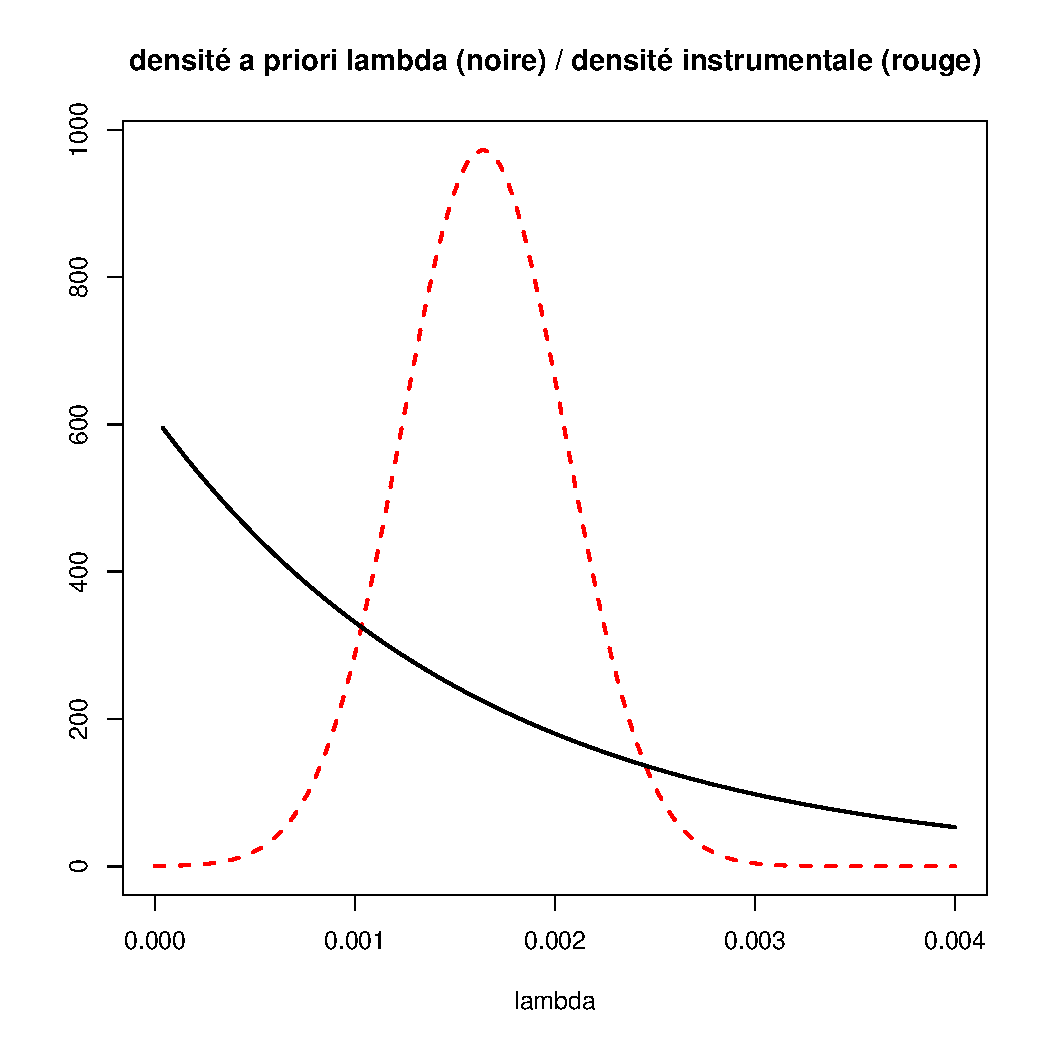
\includegraphics[width=6cm,height=5cm]{figures/calcul/prior-1.pdf} 
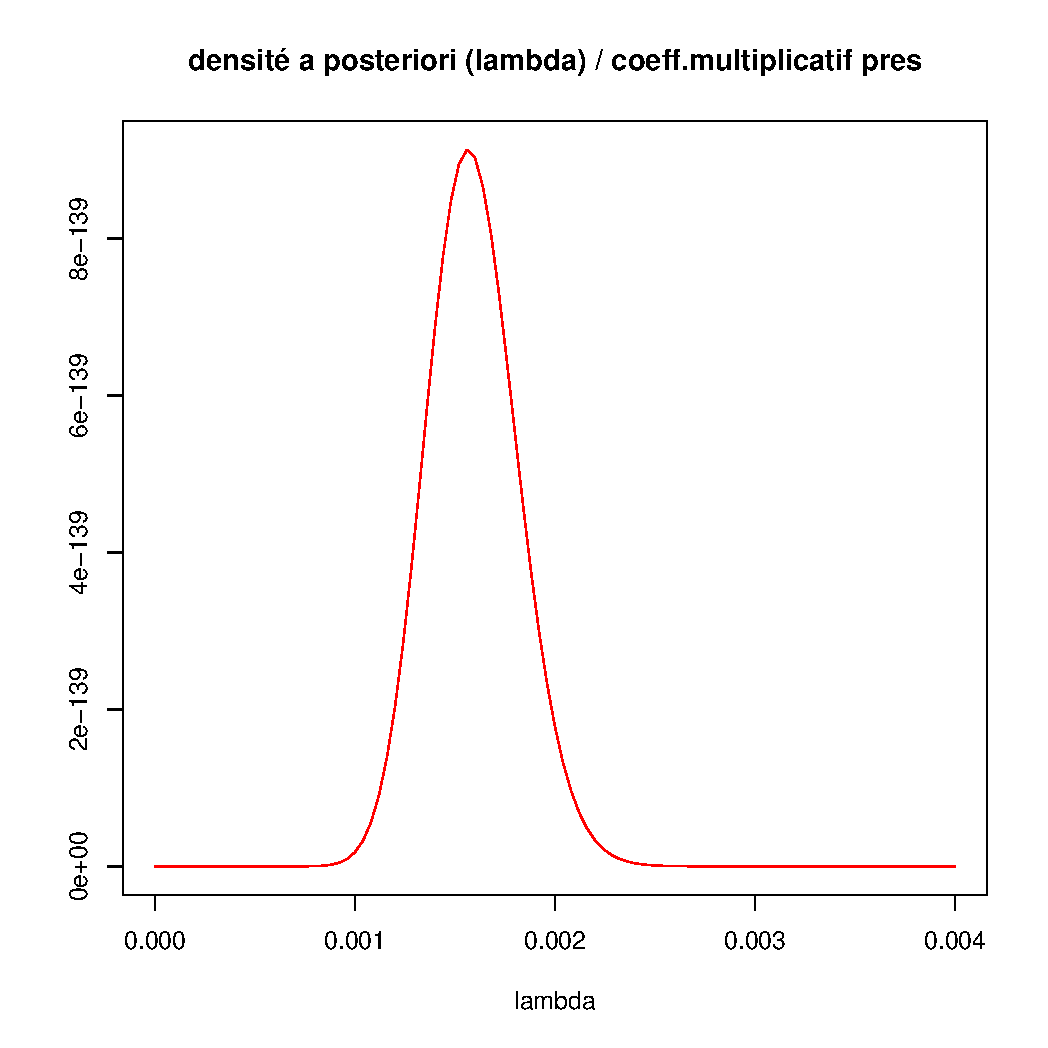
\includegraphics[width=6cm,height=5cm]{figures/calcul/posterior-1.pdf} \\
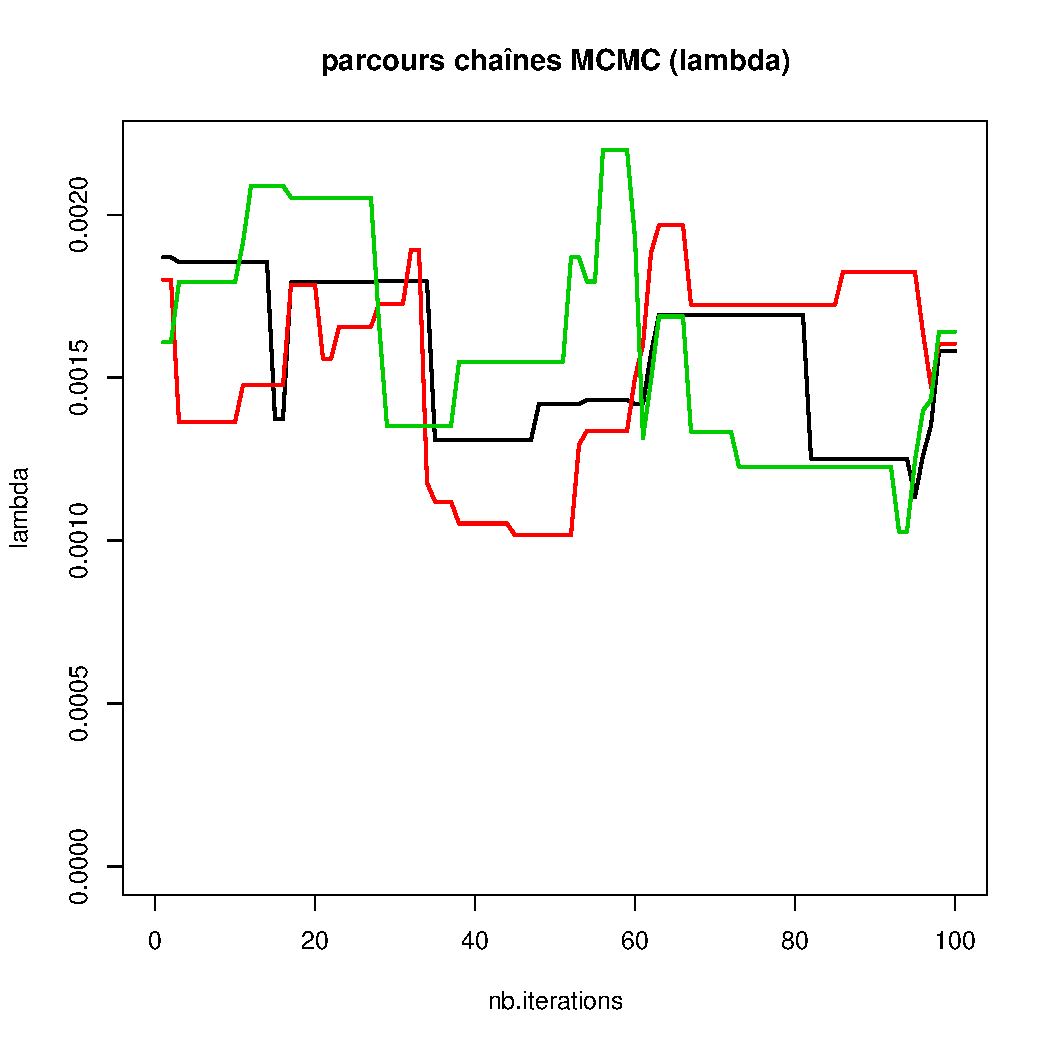
\includegraphics[width=6cm,height=5cm]{figures/calcul/MCMC1.pdf}
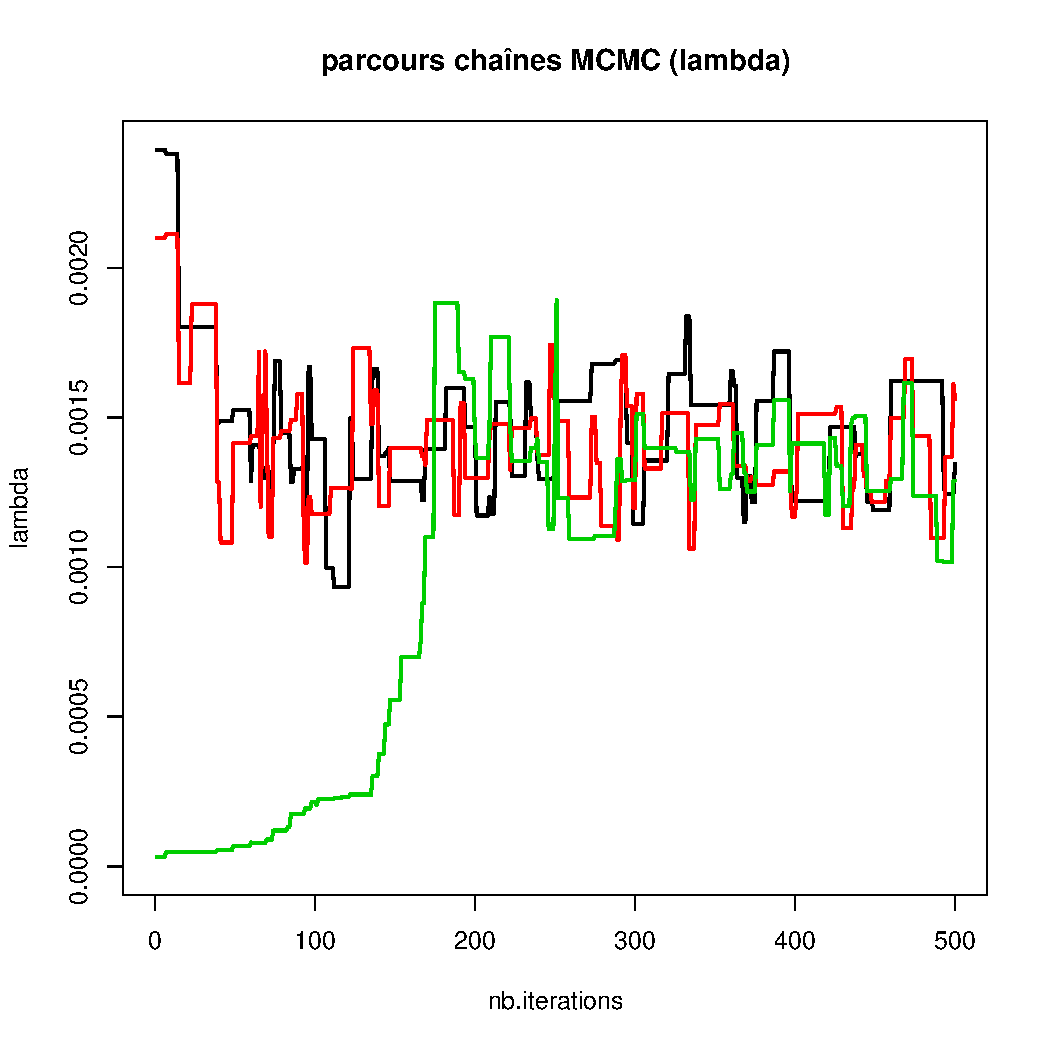
\includegraphics[width=6cm,height=5cm]{figures/calcul/MCMC2.pdf}
\end{center}
\end{rep}
\fi

\paragraph{Heuristique de progression du taux d'acception moyen $\alpha$.} Dans une chaîne MCMC produite par HM, la \emph{stationarité} est l'atteinte par une chaîne d'un tirage stationnaire dans la loi {\it a posteriori}. La rapidité de convergence vers la stationarité est induite par le taux d'acceptation $\alpha$. Au début de la MCMC, on cherche à \emph{explorer l'espace} : $\alpha$ grand ($\simeq 0.5$). Si $\alpha$ est petit, la simulation est fortement dépendante du passé de la chaîne : l'exploration de l'espace est très lente. Si $\alpha$ reste grand, chaque chaîne évolue solitairement et elles risque de se mélanger lentement. De différents travaux appliqués et théoriques, on a tiré une règle du pouce : un $\alpha=0.25$ est souvent considéré, en pratique (en particulier lorsque $\dim\Theta$ est grande) comme 
un bon objectif de renouvellement à la stationnarité. Par ailleurs, la calibration de $\rho(\theta|\theta^{(i-1)})$ (en général, le choix de sa variance) peut être en général faite de façon {\bf empirique} en ``testant" le taux d'acceptation effectif. \\

\paragraph{Heuristique de choix d'une loi instrumentale $\rho(\theta|...)$.} Dans le cas le plus simple, on choisit volontiers  $\rho(\theta|\theta^{(i-1)})=\rho(\theta)$ (\emph{loi statique}). Mais une modélisation standard est de choisir $\rho(\theta|\theta^{(i-1)})$ centrée sur $\theta^{(i-1)}$, et donc seule la variance doit être calibrée (ou le coefficient de variation). \\

\begin{exo}
Marche aléatoire $\theta \sim \theta^{(i-1)} +  \sigma \epsilon_i$ où $\epsilon_i \sim {\cal{N}}(0,1)$. \\
\end{exo}

\`A la différence du noyau, le caractère markovien de $\rho$ peut être relâché : on peut construire des $\rho$ {\bf adaptatives} en
utilisant tout le passé de la chaîne et non pas le dernier état connu $\theta^{(i-1)}$. Il existe une très vaste littérature à ce sujet, plutôt du domaine de la recherche que de la règle du pouce ou la ``boîte à outils". Là encore, on conseille de se référer à l'ouvrage \cite{Marin2007}. \\

\paragraph{Arrêt de chaîne MCMC.} Une fois que le \emph{temps de chauffe} est passée, la \emph{phase ergodique} est atteinte. De nombreux diagnostics de convergence vers la stationarité ont été proposés \cite{Cowles1996} et \emph{nécessitent d'avoir lancé plusieurs chaînes parallèles}. \`A la stationarité, ces chaînes parallèles se sont bien mélangées et ont ``oublié" le passé de chacune. Les diagnostics sont surtout \emph{visuels} : on regarde l'évolution du comportement d'une statistique informant sur la stabilité
de la distribution des $\theta$. \\

Parmi ces diagnostics de convergence, les statistiques de Gelman-Rubin (1992, cas 1D) et de Brooks-Gelman (1998, cas multidimensionnel) sont très standards : elles sont fondées sur la comparaison de variances inter et intra chaînes. \\

\begin{definition}{\bf Diagnostic de Gelman-Rubin.}
\begin{itemize}
\item Soit $P$ trajectoires (chaînes) parallèles de longueur $n$ (en pratique, $P = 3$.)
\item Soit $\theta^{(i)}_k$ la $i^{\text{ième}}$ réalisation sur la trajectoire $k$.
\item Soit $B$ l'estimateur de la \emph{variance de $\theta$ inter-chaînes}. 
\begin{eqnarray*}
B & = & \frac{n}{P-1}\sum\limits_{k=1}^P \left(\bar{\theta}_k - \bar{\theta}\right)^2
\end{eqnarray*}
avec
\begin{eqnarray*}
\bar{\theta}_k & = & \frac{1}{n}\sum\limits_{i=1}^n \theta^{(i)}_k \ \ \ \text{et} \ \ \ \bar{\theta} = \frac{1}{P} \sum\limits_{k=1}^P \bar{\theta}_k 
\end{eqnarray*}
\item soit $W$ l'estimateur de la \emph{variance de $\theta$ intra-chaînes} ({\bf ergodique})
\begin{eqnarray*}
W & = & \frac{1}{P}\sum\limits_{k=1}^P \left[\frac{1}{n-1}\sum\limits_{i=1}^n  \left({\theta}^{(i)}_k - \bar{\theta}_k\right)^2\right]
\end{eqnarray*}
\end{itemize}
Alors, { le rapport} (\emph{ statistique de Gelman-Rubin})
\begin{eqnarray*}
R & = & \frac{\frac{(n-1)}{n}W + \frac{1}{n}B}{W}
\end{eqnarray*}
{ tends vers 1 par valeurs supérieures}.
\end{definition}

En reprenant l'exemple \ref{debit.extreme}, on représente ci-dessous des exemples de trajectoires du taux d'acceptation et du  diagnostic de Brooks-Gelman, qui généralise Gelman-Rubin en tenant compte de la covariance entre dimensions d'une même chaîne. \\

\begin{center}
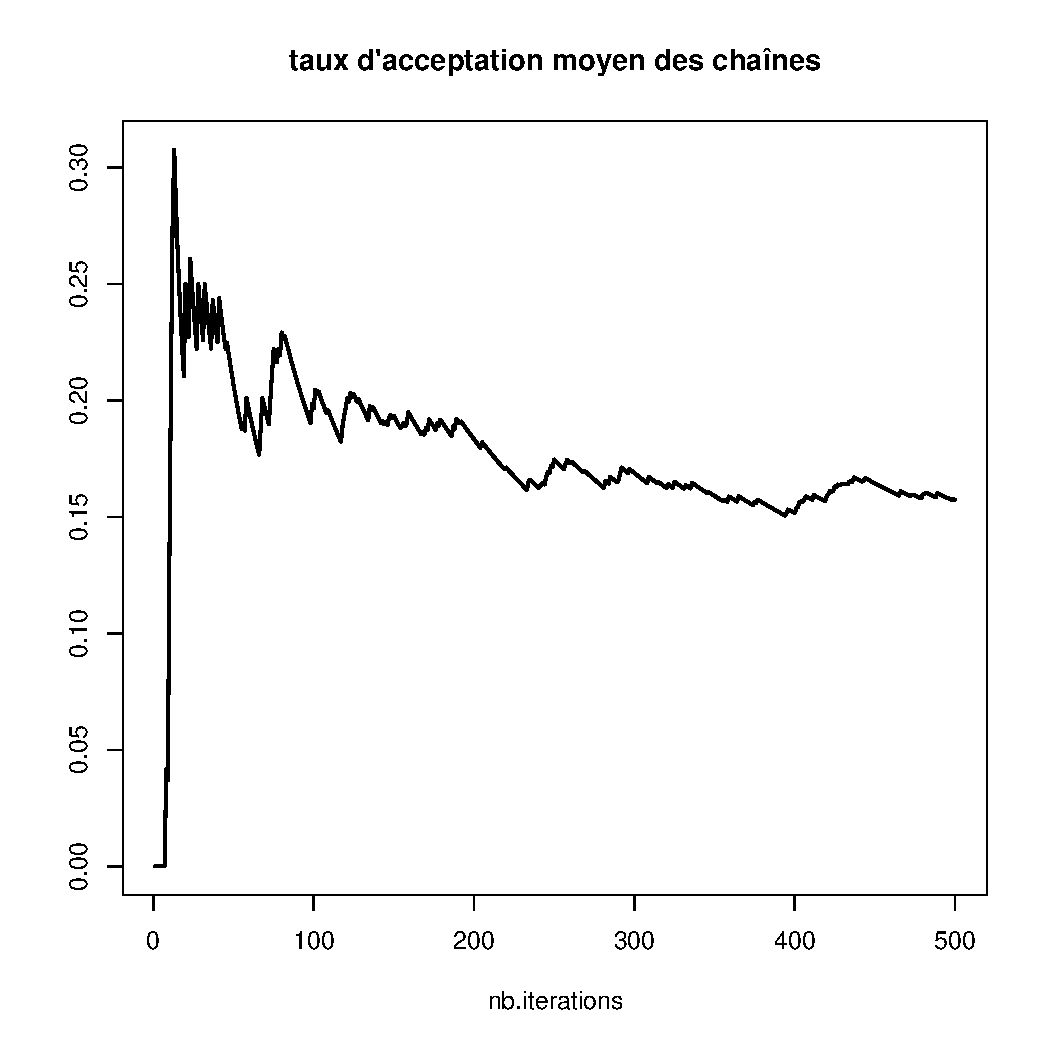
\includegraphics[width=7cm,height=7cm]{figures/calcul/alpha1.pdf}
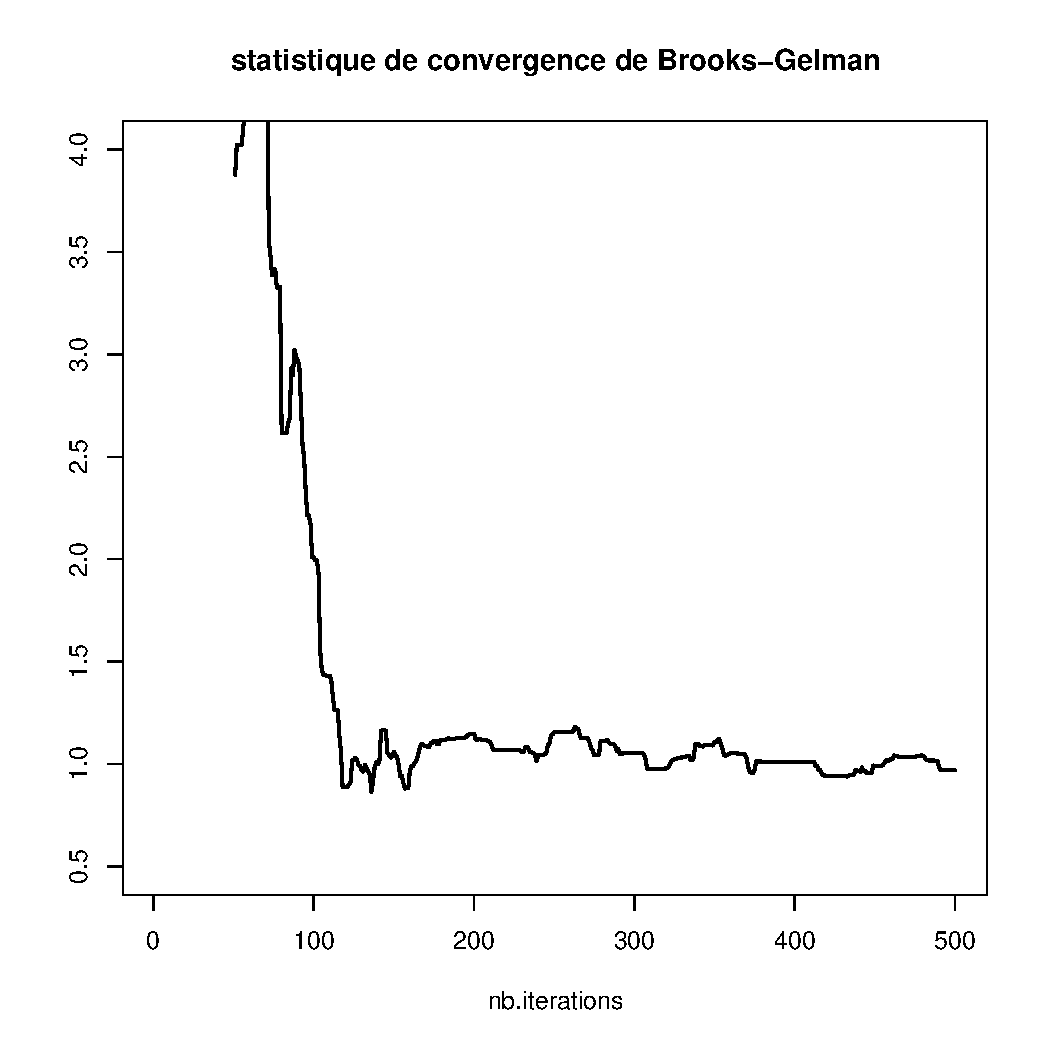
\includegraphics[width=7cm,height=7cm]{figures/calcul/bg1.pdf}
\end{center}

\paragraph{Décorrélation d'un échantillon MCMC.}
Soit $M_c$ le nombre d'itérations d'une MCMC avant qu'on atteigne la stationnarité (\textcolor{black}{\it temps de chauffe}, cf. figure \ref{ex-mcmc-1}). En sortie de la MCMC, on obtient un échantillon de $M-M_c$ vecteurs $\theta^{(M-M_c+1)},\ldots,\theta^M$
qui suivent la loi stationnaire $\pi(\theta|{\bf x_n})$. \\

\begin{figure}[!h]
\centering
\includegraphics[scale=0.45]{figures/calcul/mcmc-FR-1.jpeg}
\caption{Trois cha\^ines MCMC convergeant en parall\`ele vers la m\^eme loi-cible {\it a posteriori}. La p\'eriode de {\it chauffe} correspond au nombre d'it\'erations n\'ecessaire au m\'elange des cha\^ines, qui est un indicateur de l'atteinte de la stationnarit\'e. }
\label{ex-mcmc-1}
\end{figure} 


De par le caractère markovien de la MCMC, ces valeurs peuvent être \textcolor{black}{très dépendantes} le long d'une chaîne. Si on dispose de beaucoup de chaînes parallèles indépendantes, il suffit de prélever une valeur dans chacune... (mais c'est peu faisable en pratique). \\


 Pour obtenir un échantillon décorrélé (qui offre une meilleure information sur les caractéristiques de la loi $\pi(\theta|{\bf x_n})$), une bonne fa\c con de faire repose sur l'usage de l'\emph{autocorrélation}, de fa\c con similaire au traitement des \emph{séries temporelles}. \\
 
 On peut procéder comme suit :
 
 \begin{center}
 \begin{tabular}{|p{0.9\textwidth}|}
    \hline\\
    {{\bf Procédure de décorrélation.}
     \begin{enumerate}
\item On estime l'\textcolor{black}{autocorrélation} des éléments d'une chaîne:
\begin{eqnarray*}
\mbox{Aut}_{i,i+j} & = & \frac{\E\left[\left(\theta^{(i)} - \E[\theta|{\bf x_n}]\right)\left(\theta^{(i+j)} - \E[\theta|{\bf x_n}]\right)\right]}{\mbox{Var}[\theta|{\bf x_n}]}
\end{eqnarray*} 
à valeur dans $[-1,1]$. 

\begin{itemize}
%\item \scriptsize l'estimation empirique des quantités est faite en moyennant sur les chaînes parallèles
\item  \`A $i$ fixé, $\mbox{Aut}_{i,i+j}$ tends vers 0 lorsque $j$ augmente $\Leftrightarrow$ $\theta^{(i+j)}$ devient de plus en plus décorrélé de $\theta^{(i)}$. 
\item  On considère que cette décorrélation est effective lorsque l'estimateur de $\mbox{Aut}_{i,i+j}$ est un {\bf bruit blanc gaussien}.
\item  On peut donc, en moyenne sur les $i$, estimer le nombre d'itérations nécessaire $t$ pour obtenir 2 valeurs décorrélées de $\theta$.   
\end{itemize}


\item Sur chaque chaîne, on sélectionne le sous-échantillon ({\it thinning})
\begin{eqnarray*}
\theta^{(M-P+1)},\theta^{M-P+1+t},\theta^{M-P+1+2t},\ldots.
\end{eqnarray*}



\item On baisse encore la dépendance des éléments de l'échantillon final en prélevant dans les chaînes indépendantes. 
\end{enumerate}}  \\
\hline
    \end{tabular} 
    \end{center}
    \hspace{0.5cm}
    

\subsubsection{\'Echantillonneur de Gibbs et approches hybrides}

Dans un cas où  le param\`etre $\theta=(\theta_1,\ldots,\theta_d)$ est multidimensionnel (ce qui concerne notamment pour les mod\`eles hi\'erarchiques), il est recommand\'e d'utiliser une algorithmique d'{\it \'echantillonnage de Gibbs} \cite{Robert2004} qui tire parti du principe de \emph{cascade rule} ($\S$ \ref{multidim.sim}). \\

\'Etant donné un échantillon ${\bf x_n}$,  supposons disposer des lois {\it a posteriori} conditionnelles   
\begin{eqnarray*}
\theta_1|\theta_2,\ldots,\theta_d,{\bf x_n} & \sim & \pi(\theta_1|\theta_2,\ldots,\theta_d,{\bf x_n}), \\
\theta_2|\theta_1,\theta_3,\ldots,\theta_d,{\bf x_n} & \sim & \pi(\theta_2|\theta_1,\theta_3,\ldots,\theta_d,{\bf x_n}), \\
\ldots & & \ldots.
\end{eqnarray*} 
Alors la cha\^ine de Markov de vecteurs 
\begin{eqnarray*}
\theta^{(1)}=\left(\begin{array}{l} \theta^{(1)}_1 \\ \ldots \\ \theta^{(1)}_d\end{array}\right) \ , \hspace{0.5cm} \theta^{(i)}=\left(\begin{array}{l} \theta^{(M)}_1 \\ \ldots \\ \theta^{(M)}_d\end{array}\right) \ , \ldots
\end{eqnarray*}
produite par la simulation conditionnelle it\'er\'ee converge \'egalement vers la loi {\it a posteriori}-cible $\pi(\theta|{\bf x_n})$, sous des conditions tr\`es g\'en\'erales. \\

Lorsque les lois {\it a posteriori} conditionnelles ne sont elles-m\^emes pas compl\`etement explicites, une d\'emarche hybride, dite de {\it Metropolis-Hastings-within-Gibbs}, consiste \`a faire appel \`a un test de Metropolis pour chaque dimension.

\begin{remark} 
La solution proposée pour l'exercice \ref{debit.extreme} est d'ailleurs un exemple d'algorithme de Gibbs en dimension 2, incluant une étape de Metropolis-Hastings pour l'estimation du paramètre $\lambda$. 
\end{remark}

L'algorithmique de Gibbs (hybride), qui exploite au maximum la structure conditionnelle des modèles hiérarchiques, est donc très générale, et elle est notamment particulièrement intéressante lorsqu'on traite des \emph{problèmes à données manquantes} (ex : présentant des données censurées, ou des variables latentes comme les modèles de mélange...). Dans un cadre bayésien, il permet de considérer ces données comme des paramètres inconnus à simuler {\it ({augmentation de données})}. L'exemple suivant illustre ce procédé. 

\begin{exec}{\bf (Retour à l'exercice \ref{quasi.conjug}).}. 
 On suppose de nouveau connaître un échantillon ${\bf x_n} \sim {\cal{N}}(\theta,1)$ composé de quelques observations $x_1,\ldots,x_{n-1}$ supposées iid de loi ${\cal{N}}(\theta,1)$, et d'une  pseudo-observation $y$ qui est un cas-limite masquant ({\it censurant}) une observation $x_{n}$ qui aurait dû être faite: $y<x_{n}$. On considère toujours $\theta \sim {\cal{N}}(\mu,1)$ {\it a priori}. 
Pouvez-vous produire un algorithme d'échantillonnage par Gibbs qui génère des réalisations de la loi {\it a posteriori} de $\theta$ ? 
\end{exec}

\if\mycmdexotwo1 \vspace{1cm} \begin{rep}
Si on connaissait $x_n$, le modèle bayésien serait conjugué et
\begin{eqnarray*}
\theta|{\bf x_n} & \sim & {\cal{N}}\left(\frac{1}{n}\left(\mu + \sum\limits_{i=1}^n x_i\right),(n+1)^{-1}\right)
\end{eqnarray*}
 On considère alors la donnée manquante $x_{n}$ comme un paramètre inconnu et aléatoire.  Sachant $\theta$ et ${\bf x_n}$, on peut montrer par la règle de Bayes que la loi de la variable aléatoire manquante $X_n$ est la normale tronquée
\begin{eqnarray*}
{\cal{N}}(\theta,1)\cdot \1_{\{x_n\geq y\}}.
\end{eqnarray*}
En effet, la fonction de répartition de $X_n$ est conditionnelle : $P(X_n<x|X_n>y)$. Par la règle de Bayes
\begin{eqnarray*}
P(X_n<x|X_n>y) & = & \frac{P(X_n<x \cap X_n>y)}{P(X_n>y)} \ = \ \frac{P(y<X_n<x)}{P(X_n>y)}.
\end{eqnarray*}
Le dénominateur est une constante (indépendante de $x$). Donc
\begin{eqnarray*}
P(X_n<x|X_n>y) & \propto & \int_{y}^x f_X(u) \ du \ = \ \int_{-\infty}^x f_X(u) \1_{\{y\leq u\}} \ du
\end{eqnarray*}
où $f_X$ est la densité d'un $X$ non-contraint (ici gaussienne). On en déduit que la densité de $X_n$ est
\begin{eqnarray*}
f_{X_n}(x) & = & \frac{f(x)\1_{\{y\leq x\}}}{\int_{-\infty}^{\infty} f(u)\1_{\{y\leq u\}} \ du}.
\end{eqnarray*}

L'algorithme de Gibbs à mettre en oeuvre est donc le suivant :
\texttt{
\begin{itemize}
\item On part d'une valeur $\theta^{(0)}$
\item Itération $i\geq 1$ :
\begin{enumerate}
\item on simule $x^{(i)}_{n} \sim {\cal{N}}\left(\theta^{(i-1)},1\right)\cdot \1_{\{x_n\geq y\}}$
\item on simule $\theta^{(i)} \sim  {\cal{N}}\left(\frac{1}{n}\left(\mu + \sum\limits_{i=1}^{n-1} x_i + x^{(i)}_{n}\right),(n+1)^{-1}\right)$
\end{enumerate}
\end{itemize}
}

\end{rep}



\fi
\vspace{0.5cm}

La modélisation bayésienne par conditionnement peut fréquemment entra\^iner le mécanisme suivant : 
\begin{enumerate}
\item On construit un {\it a priori} \emph{hiérarchique}
\begin{eqnarray*}
\pi(\theta) & = & \pi(\theta_1|\theta_2,\theta_3)\pi(\theta_2|\theta_3)\pi(\theta_3)
\end{eqnarray*}
avec des {\it a priori} non-informatifs
\item Ce conditionnement est souvent choisit pour tirer parti de \emph{conjugaisons} {\it a posteriori} : les lois conditionnelles
\begin{eqnarray*}
\pi(\theta_1|{\bf x_n},\theta_2,\theta_3), \\
\pi(\theta_2|{\bf x_n},\theta_1,\theta_3), \\
\pi(\theta_3|{\bf x_n},\theta_1,\theta_2)
\end{eqnarray*}
sont explicites, ce qui permet d'utiliser un algorithme de Gibbs.
\end{enumerate}
Toutefois,  même si ces lois {\it a posteriori} \emph{conditionnelles}  sont propres, la loi \emph{jointe} peut ne pas l'être :
\begin{eqnarray*}
\int_{\Theta} \pi(\theta|{\bf x_n}) \ d\theta & = & \infty.
\end{eqnarray*}
Il est donc indispensable de vérifier la \emph{propriété} {\it a posteriori} avant de mettre en oeuvre un algorithme de Gibbs. 



\begin{exec}{\bf Modèle à effets aléatoires autour d'une constante  (Hobert-Casella).}
Pour $i=1,\ldots,I$ et $j=1,\ldots,J$, on considère 
\begin{eqnarray*}
x_{ij} &  = & \beta + u_i + \epsilon_{ij}
\end{eqnarray*}
où $u_i\sim {\cal{N}}(0,\sigma^2)$ et $\epsilon_{ij}\sim {\cal{N}}(0,\tau^2)$. Ce type de modèle permet de représenter la distribution d'une caractéristique au sein d'une population, où  $\beta$ est une tendance moyenne, $u_i$ correspond à une  variation d'un groupe et $\epsilon_{ij}$ à une  variation au sein d'un sous-groupe. On suppose choisir 
\begin{eqnarray*}
\pi(\beta,\sigma^2,\tau^2) & \propto & \frac{1}{\sigma^2\tau^2} \ \ \ \text{(prior de Jeffreys)}.
\end{eqnarray*}
On note ${\bf x_{IJ}}$ l'échantillon des données observées, $\bar{x}_i$ la moyenne sur les $j$. On note ${\bf u_I}$ l'échantillon manquant des $u_1,\ldots,u_I$ (reconstitué dans l'inférence). 
\begin{enumerate}
    \item Calculer les lois conditionnelles {\it a posteriori} de 
\begin{eqnarray*}
U_i|{\bf x_{IJ}},\beta,\sigma^2,\tau^2 &  &  \\
\beta|{\bf x_{IJ}},\sigma^2,\tau^2,{\bf u_I} &  &  \\
\sigma^2|{\bf x_{IJ}},\beta,\tau^2,{\bf u_I} &  &  \\
\tau^2|{\bf x_{IJ}},\beta,\sigma^2,{\bf u_I} & & 
\end{eqnarray*}
Ces lois sont-elles bien définies ?
\item Donner une formule (à un coefficient proportionnel près) pour la loi {\it a posteriori} jointe $\pi(\sigma^2,\tau^2|{\bf x_{IJ}})$. Comment se comporte-t-telle au voisinage de $\sigma=0$, pour $\tau\neq 0$ ? Que pouvez-vous en déduire ? 
\item Mettre en place un algorithme de Gibbs permettant d'inférer sur $(\beta,\sigma^2,\tau^2)$. 
Que pouvez-vous dire sur la convergence des chaînes MCMC ?
\end{enumerate}
\end{exec}

\if\mycmdexotwo1 \vspace{1cm} \begin{rep}
\begin{enumerate}
\item Des calculs algébriques montrent que les lois conditionnelles sont
\begin{eqnarray*}
U_i|{\bf x_{IJ}},\beta,\sigma^2,\tau^2 & \sim & {\cal{N}}\left(\frac{J(\bar{x}_i-\beta)}{J+\tau^2\sigma^{-2}},(J\tau^{-2} + \sigma^{-2})^{-1}\right) \\
\beta|{\bf x_{IJ}},\sigma^2,\tau^2,{\bf u_I} & \sim & {\cal{N}}\left(\bar{x}-\bar{u},\tau^2/IJ\right) \\
\sigma^2|{\bf x_{IJ}},\beta,\tau^2,{\bf u_I} & \sim &  {\cal{IG}}\left(I/2,(1/2)\sum\limits_{i=1}^I u^2_i\right) \ \ \ \ \ \text{\it (loi inverse gamma)} \\
\tau^2|{\bf x_{IJ}},\beta,\sigma^2,{\bf u_I} & \sim &  {\cal{IG}}\left(IJ/2,(1/2)\sum\limits_{i=1}^I\sum\limits_{j=1}^J (x_{ij} - u_i - \beta)^2\right)  
\end{eqnarray*}
qui sont donc bien définies. 
\item La loi {\it a posteriori} jointe 
\begin{eqnarray*}
\pi(\sigma^2,\tau^2|{\bf x_{IJ}}) & = & \int \pi(\beta,\sigma^2,\tau^2|{\bf x_{IJ}}) \ d\beta \\
                                  & = & \int\left[\int_1\ldots\int_i\ldots\int_I \pi(\beta,\sigma^2,\tau^2|{\bf x_{IJ}}) \ d u_i\right] d\beta \\
\end{eqnarray*}
est proportionnelle à
\begin{eqnarray*}
\frac{\sigma^{-2-I}\tau^{-2-IJ}}{\left(J\tau^{-2} + \sigma^{-2}\right)^{I/2}}\sqrt{\tau^2 + J\sigma^2} \exp\left\{-\frac{1}{2\tau^2}\sum\limits_{i,j} (y_{ij}-\bar{y}_i)^2 - \frac{J}{2'\tau^2 + J\sigma^2)}\sum\limits_{i} (\bar{y}_i-\bar{y})^2\right\}
\end{eqnarray*}
qui se comporte comme $\sigma^{-2}$ au voisinage de $\sigma=0$, pour $\tau\neq 0$. Cette loi jointe n'est donc pas intégrable ({\it propre}). 
\item On constate normalement une absence de convergence claire des chaînes, ou une stationnarité (momentanée) trompeuse.
\end{enumerate}
\end{rep}
\fi
\vspace{0.5cm}

\clearpage

\subsubsection{Un résumé de ces premières méthodes}

On trouvera sur le tableau ci-dessous quelques informations qui résument l'usage et les particularités de ces algorithmes de calcul bayésien. Pour aider à faire un choix, voici quelques conseils reposant sur quelques questions essentielles.
\begin{itemize}
\item La loi-cible {\it a posteriori} est-elle proche d'un cas explicite (ou conjuguée) (ex: loi normale censurée) ?
\item Si oui, que faudrait-il faire (typiquement, \emph{simuler des données manquantes} $\Rightarrow$ Gibbs)
\item En multidimensionnel, a-t-on des propriétés de conjugaison conditionnelles ($\Rightarrow$ Gibbs) ? 
\item Si nous n'avons aucune idée, peut-on trouver une loi $\rho(\theta)$ partageant certaines caractéristiques avec $\pi(\theta|{\bf x_n})$ ?
\begin{itemize}
\item Par exemple, on peut tenter de tracer  $\pi(\theta|{\bf x_n})$ (à un coefficient près) dans les cas unidimensionnels. 
\item On peut également mener un calcul du  mode {\it a posteriori} $\hat{\theta}$ = maximum de la vraisemblance pondérée par l'{\it a priori}.
\item une idée de loi instrumentale typique est ainsi une loi $\rho(\theta)$  gaussienne ${\cal{N}}(\hat{\theta},\sigma^2I_d)$ avec $\sigma$ calibré empiriquement. 
\end{itemize}
\end{itemize}


\begin{tabular}{l|l|l|l|l}
          & \textcolor{purple}{Acceptation -} & \textcolor{purple}{\'Echant.} & \textcolor{purple}{Métropolis -} & \textcolor{purple}{Gibbs}  \\
          & \textcolor{purple}{Rejet}         & \textcolor{purple}{d'importance} & \textcolor{purple}{Hastings (MH)}  &  \\
\hline
\emph{Contexte}  & &&& \\
\cline{1-1}
Dimension de $\theta$ & 1 & grande & grande & grande \\
Nature simulation  & iid  & non-indep.$^*$ & non-indep. approx.$^*$ & non-indep. approx.$^*$ \\
Nature algo & itératif          & statique   & itératif & itératif \\ 
& &&& \\
\emph{Nb. itérations typ.} & quelques       & 1 & quelques dizaines  & quelques \\
                                      & centaines      &   & de milliers        & milliers \\
& &&& \\
\emph{Implémentation} & aisée & aisée & calibration fine & aisée \\
                                 &       &       & de $\rho(\theta)$  nécessaire & \\
& &&& \\
\emph{Critère d'arrêt} & aucun & aucun   & nécessaire   & nécessaire \\
& &&& \\
\textcolor{red}{Risques} & fort taux  & poids mal   & mauvais mélange   & nécessite souvent \\
            & de rejet                     &  équilibrés           &   chaînes //                       & couplage avec M-H \\
& &&& \\
\textcolor{red}{Temps de calcul} & long & rapide & long & plut\^ot rapide \\
\hline
\end{tabular}

%%%%%%%%%%%%%%%%%%%%%%%%%%%%%%%%%%%%%%
\clearpage
\subsection{Méthodes d'échantillonnage accélérées}

Les méthodes MCMC ont été et restent très utilisées pour simuler des valeurs {\it a posteriori} $\theta_1,\ldots,\theta_n \overset{iid}{\sim} \pi(\theta|x)\propto f(x|\theta)\pi(\theta)$. Elles sont toutefois lentes pour des problèmes complexes, et la convergence vers la loi-limite ({\it a posteriori} dans un cadre bayésien) reste difficile à vérifier. En particulier, les \emph{méthodes MCMC restent très lourdes} (voire impossibles) à utiliser dans les problèmes de type ``Big Data". \\

\begin{exo}
Modèles à états latents, tels les modèles de Markov cachés permettant de segmenter des images structurées de fa\c con non supervisée... \\
\end{exo}

Ainsi, des avancées importantes pour {\bf accélérer les algorithmes d'échantillonnage} ont été menées :
\begin{itemize}
\item en se fondant sur des techniques de \emph{réduction de variance} ; 
\item en démarrant les chaînes de Markov \emph{au plus proche du mode {\it a posteriori}}  ; 
\item en \emph{améliorant le choix des lois instrumentales}, inspirées par la physique énergétique (dynamique, particules, quantique...).
\end{itemize}
Nous en listons ci-dessous quelques-unes. \\

\noindent Soulignons cependant que dans un cadre d'usage de plus en plus soumis aux contraintes de grande dimensionalité et d'apprentissage massif, dans la réalité des faits, on calcule rarement la distribution {\it posteriori}. On préfère se simplifier la vie et les calculs en approximant la loi distribution {\it posteriori} par une valeur unique (\texcolor{black}{mode a posteriori}). Il s'agit ni plus ni moins d'une \emph{maximisation de vraisemblance pénalisée} (voir $\S$ \ref{estimation.MAP.ML} pour plus de détails). Dans ce contexte, les les \emph{techniques d'optimisation}, comme l'algorithme EM ou le Gradient Boosting,  ont encore de beaux jours devant elle, et il est possible d'interpréter ces algorithmes comme des approches "dégénératives" du cadre MCMC.   


\subsubsection{Réduction de variance par utilisation des corrélations négatives (variables antithétiques)}

Considérons deux échantillons iid $(\theta_1,\ldots,\theta_m)$ et $(\tilde{\theta}_1,\ldots,\tilde{\theta}_m)$ suivant $\pi(\theta|D)$ pour estimer
$$
{\cal{H}} = \int_{\R} h(\theta) \pi(\theta|D) \ d\theta.
$$
Soient
$$
\hat{\cal{H}}_1 = \frac{1}{m} \sum\limits_{i=1}^m h(\theta_i)  \ \ \  \ \text{et} \ \ \ \ \hat{\cal{H}}_2 = \frac{1}{m} \sum\limits_{i=1}^m h(\tilde{\theta}_i)
$$
de moyenne $m$ et de variance $\sigma^2$. Alors, la variance de la moyenne vaut
$$
\V\left[\frac{1}{2}\left(\hat{\cal{H}}_1+ \hat{\cal{H}}_2\right) \right]  = \frac{\sigma^2}{2} + \frac{1}{2} \mbox{Cov}\left(\hat{\cal{H}}_1,\hat{\cal{H}}_2 \right)
$$
Par conséquent, si les deux échantillons sont \emph{négativement corrélés}, 
$$
\mbox{Cov}\left(\hat{\cal{H}}_1,\hat{\cal{H}}_2 \right) \leq 0
$$
ils font mieux que deux échantillons de même taille. Ce type d'approche a été formalisé sous le nom de \emph{réduction de variance par variables antithétiques} :
\begin{enumerate}
\item Si $\pi(\theta|D)$ symétrique autour de $\mu$, prendre $\tide{\theta}_i = 2\mu- \theta_i$ ; 
\item Si $\theta_i = F^{-1}(U_i)$, prendre $Y_i = F^{-1}(1-U_i)$ ; 
\item Si $(A_i)_i$ est une partition de $\Theta$, produire un échantillonnage \emph{partitionné} (ou  \emph{stratifié}) en choisissant des $\theta_j$ dans chaque $A_i$ (nécessite de connaître $\Pi(A_i)$).
\end{enumerate}


\subsubsection{Variables de contrôle}

Soit
$$
{\cal{H}} = \int_{\R} h(\theta) \pi(\theta|D) \ d\theta
$$
à évaluer et 
$$
{\cal{H}}_0 = \int_{\R} h_0(\theta) \pi(\theta|D) \ d\theta
$$
connue. On estime quand même ${\cal{H}}_0$ par $\hat{\cal{H}}_0$ (et ${\cal{H}}$ par $\hat{\cal{H}}$). Dans ce cas, on peut définir un {\bf estimateur combiné} :
$$
\hat{\cal{H}}^* =  \hat{\cal{H}} + \beta\left(\hat{\cal{H}}_0-{\cal{H}}_0\right)
$$

\begin{proposition}
$\hat{\cal{H}}^*$ est sans biais pour ${\cal{H}}$ et 
$$
\V\left[\hat{\cal{H}}^* \right] = \V\left[\hat{\cal{H}} \right] + \beta^2  \V\left[\hat{\cal{H}}_0 \right] + 2\beta \mbox{Cov}\left(\hat{\cal{H}} ,\hat{\cal{H}}_0 \right).$$
\end{proposition}

On peut alors faire un choix optimal de $\beta$, qui permet de diminuer la variance de l'estimateur :
$$
 \beta^* = - \frac{\mbox{Cov} \left(\hat{\cal{H}} ,\hat{\cal{H}}_0 \right)}{\V\left[\hat{\cal{H}}_0 \right]} 
$$
avec  
$$
\V\left[\hat{\cal{H}}^* \right] =  \V\left[\hat{\cal{H}} \right] \left(1-\rho^2\right)
$$
où $\rho^2$ est le coefficient de corrélation entre $\hat{\cal{H}}$ et $\hat{\cal{H}}_0$. \\

\begin{exo}{\bf Approximation de quantile.}
Supposons vouloir évaluer 
$$
q = \Pi(\theta>a|D) \ = \ \int_a^{\infty} \pi(\theta|D) \ d\theta
$$
par
$$
\hat{q} = \frac{1}{n} \sum\limits_{i=1}^n \1_{\{\theta_i > a\}}, \ \ \ \ \ \theta_i \overset{iid}{\sim} \pi(\theta|D)
$$
avec
$
\Pi(\theta>\mu|D) = 1/2
$. La variable de contrôle
$$
\frac{1}{n} \sum\limits_{i=1}^n \1_{\{\theta_i > a\}} + \beta\left(\frac{1}{n} \sum\limits_{i=1}^n \1_{\{\theta_i > \mu\}} - \Pi(\theta>\mu|D)\right)
$$
améliore $\hat{q}$ si
$$
\beta < 0 \ \ \ \ \text{et} \ \ \ \ |\beta|<2\frac{\Pi(\theta>a|D)}{\Pi(\theta>\mu|D)}.
$$


\end{exo}


\subsubsection{Rao-Blackwellisation}

On peut également vouloir tirer parti de l'inégalité 
$$
\V\left[\E[h(\theta)|Y]\right] \leq \V\left[h(\theta)\right],
$$
aussi appelée \emph{Théorème de Rao-Blackwell}, pour diminuer la variance d'un estimateur de Monte Carlo. 

\begin{proposition}
Si $\hat{\cal{H}}$ est un estimateur sans biais de ${\cal{H}}=\E_{\pi}\left[h(\theta)\right]$, avec $\theta$ simulé à partir de la densité jointe $\tilde{\pi}(\theta,y)$ où
$$
\int \tilde{\pi}(\theta,y) \ dy = \pi(\theta)
$$
alors l'estimateur
$$
\hat{\cal{H}}^* = \E_{\tilde{\pi}}\left[\hat{\cal{H}}|Y_1,\ldots,Y_n \right] 
$$
domine $\hat{\cal{H}}(\theta_1,\ldots,\theta_n)$ en variance (et est aussi sans biais).
\end{proposition}

L'algorithme EM, notamment, tire parti de ce procédé pour maximiser une vraisemblance de données incluant des données manquantes. 



%%%%%%%%%%%%%%%%%%%%%%%%%%%%%%%%%%%%%%
\subsubsection{Amélioration de lois instrumentales par dynamique de Langevin / hamiltonienne}

Les améliorations de lois instrumentales au sein des algorithmes de type MCMC sont généralement fondées sur des parallèles avec des problèmes de \emph{diffusion} / \emph{mouvement de système physique}  (particulaire), régis par des équations aux dérivées partielles (EDP). L'idée générale est d'utiliser de l'information sur la densité cible au travers du passé de l'algorithme, et plus précisément l'information contenue dans le \emph{gradient $\nabla \log \pi(\theta|D)$}. Le cadre général de la dynamique particulaire de Langevin offre une formalisation de ce problème. Par la suite, pour simplifier les notations, on notera $D$ les données disponibles. \\

\begin{proposition}{\bf Metropolis-Adjusted Langevin Algorithm (MALA)}
Discrétisation d'une diffusion de Langevin de probabilité stationnaire $\pi(\theta|D)$ :
\begin{eqnarray*}
\rho(\theta,.) & = & {\cal{N}}_d\left(\theta + \frac{h^2}{2}\nabla \log \pi(\theta|D), h^2 I_d\right)
\end{eqnarray*}
pour un pas $h>0$. Le choix de $h$ relève de considérations sur la structure de $\mbox{Cov}(\theta|D)$.
\end{proposition}

De fa\c con plus explicite, on veut simuler selon une loi non normalisée définie en termes de potentiel
$$
\pi(\theta|D)  \propto  \exp\left(-U(\theta)\right).
$$
Sous des conditions peu contraignantes, cette densité est l'unique mesure de probabilité invariante d'une \emph{équation différentielle stochastique de Langevin}
$$
\mbox{d}\theta_t  =  -\nablaU(\theta_t) \mbox{d}t + \sqrt{2}\mbox{d} B_t
$$
avec $B_t$ un processus brownien (qui décrit le mouvement d'une particule soumise à une infinité de chocs en des temps très courts)
$$
B_t \sim {\cal{N}}(0,t). 
$$
 En général on ne peut résoudre exactement l'équation précédente : on s'appuie alors sur l'approximation produite par une discrétisation d'Euler-Maruyama
$$
\theta_{k+1} = \theta_k - \gamma\nabla U(\theta_k) +  \sqrt{2\gamma} Z_{k+1}.
$$
Cette approche est l'\emph{Unadjusted Langevin Algorithm} (ULA) et s'appelle aussi \emph{Langevin Monte Carlo} (LMC). Il s'agit simplement d'un calcul de MAP par un algorithme de descente de gradient avec du bruit ajouté à chaque itération.
Des résultats théoriques ont été obtenus récemment pour contrôler l'erreur d'approximation / taille d'échantillon et dimension (si $\pi(\theta|D)$ régulière),par Dumus et Moulines (2017). Cette approche marche bien pour le traitement de la grande dimension de $\theta$ en inférence bayésienne. \\

Toutefois, cette discrétisation induit du biais, qui peut être ôté par une étape d'acceptation-rejet de Metropolis-Hastings, ce qui donne la formulation MALA de l'algorithme. L'algorithmique MALA hérite donc des bonnes propriétés de convergence de ULA et affronte bien la grande dimension. Dans un tour d'horizon récent, Nemeth et Fearnhead (2019) ont récemment montré que le pas optimal pour MALA est grand, mais MALA coûte plus cher par itération que les approches ULA. Par ailleurs, les lois instrumentales fondées sur ULA ont un meilleur taux d'acceptation que les marches aléatoires MALA. \\

\paragraph{Approche MYULA.} Quand $\pi(\theta|D)$ n'est pas régulière, on suppose que le potentiel peut s'écrire
$$
U(\theta) = f(\theta) + g(\theta)
$$
où $f$ est convexe, continûment différentiable, et de gradient lipschitzien ; $g$ est propre, convexe, et semi-continue à gauche. On peut alors remplacer $g$ par son enveloppe dite de Moreau-Yosida (voir figure \ref{MY}) :
\begin{eqnarray*}
g^{\lambda}(x) & = & \min\limits_{y\in \R^d} \left\{ g(y) + (2\lambda)^{-1} \|x-y\l^2\right\} \\
\nabla g^{\lambda}(x) & = & \lambda^{-1} \left(x-\mbox{prox}^{\lambda}_g(x)\right)
\end{eqnarray*}
avec
$$
\mbox{prox}^{\lambda}_g(x) = \arg\min\limits_{y\in \R^d} \left\{ g(y) + (2\lambda)^{-1} \|x-y\l^2\right\}. 
$$
L'algorithme de \emph{Moreau-Yosida ULA} (MYULA) s'écrit alors
$$
\theta_{k+1} = \left(1-\frac{\gamma}{\lambda}\right)\theta_k - \gamma\nabla f(\theta_k) + \frac{\gamma}{\lambda}\mbox{prox}^{\lambda}_g(\theta_k) + \sqrt{2\gamma} Z_{k+1}.
$$

\begin{figure}[hbtp]
\centering
\includegraphics[scale=0.4]{figures/calcul/unif11.png} 
\caption{Illustration issue de Nemeth et Fearnhead (2019).}
\label{MY}
\end{figure}

En général, avec $\pi(\theta|D) \propto \pi(\theta) \prod\limits_{i=1}^n f(x_i | \theta)$, on a
$$
U  = \sum\limits_{i=0}^n U_i
$$
avec $U_0(\theta)=-\log \pi(\theta)$ et $U_i(\theta) = -\log f(x_i | \theta)$. Le problème posé par cet algorithme est qu'une seule itération reste coûteuse.  L'idée est d'utiliser des approches de \emph{descente de gradient stochastique} (SGD) pour accélérer le calcul. \\

\paragraph{Descente de gradient stochastique (SGD).} La version "Langevin" du SGD ({\it Stochastic Gradient Langevin Dynamics}, ou SGLD) s'écrit simplement 
$$
\theta_{k+1} = \theta_k -  \gamma\left(\nabla U_0(\theta_k) + \frac{n}{p}\sum\limits_{i\in S_{k+1}}\nabla U_i(\theta_k)\right)  + \sqrt{2\gamma} Z_{k+1}.
$$
Cette approche obtient un très faible coût de calcul par itération si $p\ll n$. Il s'agit donc, en résumé, d'un calcul de MAP par un algorithme de descente de gradient avec du bruit ajouté à chaque itération, à l'image de ce qui est massivement utilisé en apprentissage statistique. Des résultats théoriques prouvant la bonne convergence de ce type d'algorithme ont été obtenus récemment par Brosse {\it et al.} (2018). \\

\paragraph{Autres variantes.} On peut hybrider le SGLD avec une approche par \emph{variables de contrôle} si on peut estimer  le mode  de $\pi(\theta|D)$. De telles approches se nomment \emph{SGLD Control Variate} (SGLDCV) ou \emph{SGLD Fixed Point} (SGLDFP). Elles nécessitent très souvent de lancer un premier SGLD pour estimer le mode, puis opèrent un raffinement. D'autres approches s'hybridant avec des techniques d'échantillonnage d'importance (ou stratifié, par exemple) existent également.  


\paragraph{Méthodes de Monte Carlo Hamiltoniennes (HMC).}
Les méthodes HMC, disponibles sous Python 3 (\texttt{PyMC}\footnote{\url{https://colcarroll.github.io/hamiltonian_monte_carlo_talk/bayes_talk.html}}) ou \texttt{STAN}\footnote{\url{https://mc-stan.org}}, sont des méthodes MCMC issues d'un parallèle entre deux problèmes :
\begin{itemize} 
\item produire une dynamique pour la chaîne de Markov $\theta_i,\ldots,\theta_j$ s'approchant de la loi visée $\pi(\theta|{\bf x_n})$ ;
\item prévoir le mouvement d'un système physique  soumis à une \emph{dynamique hamiltonienne}.
\end{itemize}
La dynamique hamiltonienne est une reformulation de la mécanique newtonienne selon laquelle la description d'un système est faite au travers de \emph{coordonnées} (généralisées) et de \emph{momentum} (quantité de mouvement), reliées par un {\bf lagrangien} ; celui-ci exprime une différence entre énergie cinétique et énergie potentielle. Le lagrangien est une fonction des variables dynamiques qui permet d'écrire les équations de mouvement. La transformée de Legendre de ce lagrangien est nommé \emph{hamiltonien}. Le tableau ci-dessous résume la correspondance algébrique entre les deux problèmes mentionnés :

\begin{center}
\begin{tabular}{l|l}
\hline
Système physique & Applications MCMC \\
\hline
Position & $\theta$ \\
\'Energie potentielle & $ -\log \pi(\theta|D)$ \\
Momentum & Variables introduites artificiellement \\
& (variables gaussiennes en général) \\
\hline
\end{tabular}
\end{center}

L'idée générale de l'application aux MCMC est la suivante : à chaque pas de la MCMC, on met à jour les momentum et on produit une nouvelle trajectoire-candidate pour $\theta$ (et non un simple tirage) suivant une dynamique hamiltonienne (approche {\it leapfrog}). \\

Un récapitulatif rapide des méthodes fondées sur un parallèle avec des modèles de  dynamique est présenté dans le résumé ci-dessous : \\

%\begin{figure}[hbtp]
\begin{center}
\fbox{\includegraphics[scale=0.2]{figures/calcul/langevin1.png}} 
%\caption{Illustration issue de Nemeth et Fearnhead (2019).}
%\label{MY}
%\end{figure}
\end{center}


Achevons cette section par une vision des possibilités d'application de ces méthodes en {\it machine learning} (ML) et en {\it deep learning} (DL) : 

{\bf ML} :
\begin{itemize}
\item Régression logistique (dimension $d=123$) {\tiny [Welling \& Teh 2011]}
\item Débruitage d'image et déconvolution  ($d=256\times 256$) {\tiny [Durmus et al.  2018]}
\item Régression  ($d\in[2,90]) \times 256$) {\tiny [Dubeys et al.  2016]}
\item Factorisation de matrice ($d=256\times 140$) {\tiny [Simsekli et al.  2016]}
\end{itemize}

\vs {\bf DL} :
\begin{itemize}
\item Approches ensemblistes (dimension $d\in[100,600]$) {\tiny [Lakshminarayanan et al. 2017]}
\item Incertitude des poids  ($d=1200$) {\tiny [Li et al.  2016]}
\end{itemize}


%%%%%%%%%%%%%%%%%%%%%%%%%%%%%%%%%%%%%%
\subsection{Méthodes particulaires}

Le principe des méthodes particulaires est de simuler $N$ chaînes de Markov en parallèle, en éliminant celles qui restent loin du mode {\it a posteriori} et en multipliant (reproduisant) celles qui en sont proches (cf. figure \ref{particle}). \\

\begin{figure}[h!]
\centering
\includegraphics[scale=0.3]{figures/calcul/particle.png}
\caption{Plusieurs étapes typiques d'une méthode particulaire (extrait de Parent et Bernier, 2007).}
\label{particle}
\end{figure}


%%%%%%%%%%%%%%%%%%%%%%%%%%%%%%%%%%%%%%
\subsection{Méthodes variationnelles}


\subsubsection{Principe fondamental}

Les \emph{méthodes d'inférence variationnelles} placent le problème d'inférence bayésienne dans un cadre d'optimisation déterministe qui approxime la distribution-cible $\pi(\theta|x)\propto f(x|\theta)\pi(\theta)$ avec une distribution plus simple $g(\theta|\hat{\lambda})$ à manier, en minimisant une divergence de Kullback-Leibler 
\begin{eqnarray}
g(\theta|\hat{\lambda})  & = & \arg\min\limits_{\lambda} KL\left( \pi(.|x) \| g(.|\lambda) \right) \label{def.var}
\end{eqnarray}
ou
\begin{eqnarray*}
g(\theta|\hat{\lambda})  & = & \arg\min\limits_{\lambda} KL\left(  g(.|\lambda) \| \pi(.|x) \right).
\end{eqnarray*}
Notons qu'on n'écrit pas $\theta$ dans l'expression ci-dessus car KL est indépendant de tout choix de paramétrisation $h(\theta)$ avec $h$ bijectif. \\

\begin{remark}
Remarquons que si nous supposions posséder quand même un échantillon $\theta_1,\ldots,\theta_n \overset{iid}{\sim} \pi(\theta|x)$, alors 
\begin{eqnarray*}
\min\limits_{\lambda} KL\left( \pi(.|x) \| g(.|\lambda) \right) & = & \min\limits_{\lambda}  \E_{\pi(.|x)}\left[\log \frac{\pi(\theta|x)}{g(\theta|\lambda)}\right] \ = \  \max\limits_{\lambda} \E_{\pi(.|x)}\left[\log {g(\theta|\lambda)}\right] \\
%& \simeq & \max\limits_{\lambda} \frac{1}{M}\sum\limits_{i=1}^M \log {g(\theta_i|\lambda)} \ \ \ \ \text{(estimateur de Monte Carlo)} \\
& \simeq & \max\limits_{\lambda} \frac{1}{M} \underbrace{\sum\limits_{i=1}^M \log {g(\theta_i|\lambda)}}_{\text{\tiny log-vraisemblance}} \ \ \ \ \text{(estimateur de Monte Carlo).} 
\end{eqnarray*}
En d'autres termes, la meilleure approximation possible au sens de KL, sachant le choix de modèle $g(\theta|\lambda)$, est le modèle $g(\theta|\hat{\lambda})$ où $\hat{\lambda}$ est l'estimateur du maximum de vraisemblance (EMV) des données   
$\theta_1,\ldots,\theta_n$.  Cela permet de montrer d'ailleurs que l'EMV est invariant par reparamétrisation. 
\end{remark}

On s'attendrait, dans l'expression (\ref{def.var}), à utiliser la divergence KL dans le sens précédent :
\begin{eqnarray*}
KL_1(g) & = &  KL\left( \pi(.|x) \| g(.|\lambda) \right)
\end{eqnarray*}
car la loi supposée être la ``bonne" (\textit{target}) est   $\pi(\theta|x)$ : $KL_1(g)$ offre une \emph{quantification de l'erreur informationnelle} résultant de l'approximation de $\pi(\theta|x)$ par $g(\theta|\lambda)$. Cependant, la théorie variationnelle bayésienne considère en général la divergence KL dans l'autre sens :
\begin{eqnarray*}
KL_2(g) & = &  KL\left( g(.|\lambda) \| \pi(.|x) \right)
\end{eqnarray*}
En effet, cette approche  est plus simple d'un point de vue calculatoire, et permet de préférer une approximation de $\pi(.|x)$ pour lesquelles les régions de haute densité (de $g(.|\lambda)$) sont les plus correctes. Elle permet en outre de construire des \emph{bornes variationnelles} permettant de transformer le calcul de la \emph{vraisemblance marginale} ou {\it évidence}
\begin{eqnarray*}
f(x) & = & \int_{\Theta} f(x|\theta) \pi(\theta) \ d\theta \ = \ \int_{\Theta} \pi(x,\theta) \ d\theta
\end{eqnarray*}
en un problème d'optimisation (voir Fox et Roberts (2012) pour une revue détaillée). En effet, d'après l'inégalité de Jensen, pour toute densité $g(\theta|\lambda)$ de support $\Theta$,
\begin{eqnarray*}
- KL(g(.|\lambda) \| \pi(x,.)) \ = \ \int_{\Theta} g(\theta|\lambda) \log \frac{\pi(x,\theta) }{g(\theta|\lambda)} \ d\theta & \leq & \log \int_{\Theta} g(\theta|\lambda) \frac{\pi(x,\theta) }{g(\theta|\lambda)} \\
& \leq  & \log \int_{\Theta}  \pi(x,\theta)  \ =  \ \log f(x)
\end{eqnarray*}
avec égalité si $g(\theta|\lambda)=\pi(\theta|x)$.  %(voir par exemple \cite{Keribin2009})
De plus
\begin{eqnarray*}
\log f(x) & = & \underbrace{- KL(g(.|\lambda) \| \pi(x,.))}_{\text{\tiny énergie libre ${\cal{F}}(g)$}} + KL(g(.|\lambda) \| \pi(.|x)).
\end{eqnarray*}
Si on maximise l'énergie libre ${\cal{F}}(g)$ en $g(.|\lambda)$, on maximise une borne inférieure de $f(x)$, et plus celle-ci s'accroît, plus on se rapproche d'une situation où   $KL(g(.|\lambda) \| \pi(.|x))$ est faible $\Rightarrow$ \emph{$g(\theta|\lambda)$ devient géométriquement proche de la loi-cible $\pi(\theta|x)$, indépendamment de la paramétrisation $\theta$}. \\

\subsubsection{Principes d'usage}

\paragraph{\bf Approximation champ moyen.} L'approximation en champ moyen permet de faciliter la maximisation de ${\cal{F}}(g)$ lorsque le modèle est de Markov caché  (ex : traitement d'images). Dans ce cas, $\theta=(\theta_0,z)$ où $z$ est un ensemble de variables latentes $z_1,\ldots,z_M$. On peut supposer par exemple adopter une approche \emph{\it par séparabilité} ou \emph{\it composite} simplifiant le problème :
\begin{eqnarray*}
g(\theta|\lambda) & = & g_{0}(\theta_0|\lambda_0) \prod\limits_{i=1}^M g_z(z_i|\lambda_i).
\end{eqnarray*}

\paragraph{\bf Algorithme bayésien variationnel (VBEM).} L'\emph{algorithme bayésien variationnel} (Beal, 2003) maximise itérativement l'énergie libre ${\cal{F}}(g)$ par rapport aux distributions $g_z(z_i|\lambda_i)$ (étape VBE) puis $g_{0}(\theta_0|\lambda_0)$ (étape VBM). Dans ce cadre, les observations ne sont pas obligatoirement iid (comme en théorie champ moyen généralement). Cet algorithme est en fait réduit à \emph{l'algorithme EM}  si $g_{0}(\theta_0|\lambda_0)$ est la loi de l'estimateur du maximum de vraisemblance de la vraisemblance complète (les données latentes $z$ étant alors connues). Toutefois, ce type d'approche est parfois hautement simplificateur : les lois obtenues ressemblent peu aux vrais posteriors. \\

L'approximation bayésienne variationnelle a donné cours à de nombreux travaux et a été initialement appliquée à différents modèles : 
\begin{itemize}
\item modèles de mélange (Wang et Titterington); 
\item modèles à espace d'états (Wang et Titterington) ; 
\item modèles graphiques (Attias, Jordan, Beal et Ghahramani) ; 
\item réseaux de neurones (Titterington, etc.).
\end{itemize}
Ces dernières années, le développement d'algorithmes du type SVGD (\textit{Stein Variational Gradient Descent} (Liu {\it et al.} 2016), ce genre de technique s'est fortement répandu en optimisation de réseaux de neurones.  

%%%%%%%%%%%%%%%%%%%%%%%%%%%%%%%%%%%%%%
\subsection{Méthodes d'échantillonnage sans vraisemblance (ABC)}

Nous citons pour information les méthodes ABC (\textit{Approximate Bayesian Computation}) forment une famille de méthodes s'attaquant à des problèmes bayésiens pour lesquels la vraisemblance est très difficilement (voire pas du tout) manipulable (calculable). Elles se fondent sur un principe très simple d'acceptation-rejet de $\theta$ dans un ensemble évolutif de lois instrumentales, le test statistique étant assuré par un choix de statistiques supposées représentatives. \\

De tels problèmes concernent typiquement des  données spatio-temporelles complexes, des données excessivement bruitées et dépendantes ou encore des modèles stochastiques implicites (ex : modèles évolutifs de population). Dans tous les cas, nous partirons du postulat que si la vraisemblance n'est pas calculable, il est par contre aisé de simuler des variables synthétiques $X$ à partir de tirages de $\theta$. \\

%\begin{exo}{\bf Données trajectorielles.}

%\end{exo}



%%%%%%%%%%%%%%%%%%%%%%%%%%%%%%%%%%%%%%
%\subsection{Méthodes de quadrature}


%%%%%%%%%%%%%%%%%%%%%%%%%%%%%%%%%%%%%%
\subsection{Vérification {\it a posteriori}}

La vérification {\it a posteriori} regroupe l'ensemble des techniques visant à faciliter le choix d'un modèle bayésien, en particulier lorsqu'on souhaite faire varier les choix {\it a priori}. La \emph{validation} repose grossièrement sur des techniques de \emph(contrôle {\it a posteriori prédictif}. 

\begin{definition}{\bf Contrôle {\it a posteriori} prédictif.}
Un  \emph{contrôle a posteriori prédictif} est un ensemble de comparaisons entre les données initiales $x_1,\ldots,x_n$ (au travers d'une statistique résumée éventuellement) et la loi prédictive {\it a posteriori}
\begin{eqnarray*}
f(x|x_1,\ldots,x_n) & = & \int_{\Theta} f(x|\theta) \pi(\theta|x_1,\ldots,x_n) \ d\theta.
\end{eqnarray*}
\end{definition}

Les contrôles a posteriori prédictifs sont utiles pour évaluer si votre modèle vous donne des prédictions "valables" sur la réalité - correspondent-elles ou non aux données observées ? Il s'agit d'une phase utile de construction et de vérification de modèle ; elle ne vous donne pas de réponse définitive sur si votre modèle est "ok" ou s'il est "meilleur" qu'un autre modèle, cependant, elle peut vous aider à vérifier si votre modèle fait sens. \\

Cependant, les contrôles a posteriori prédictifs  impliquent une double utilisation des données, ce qui viole le principe de vraisemblance. Ils peuvent cependant être utilisés si l'utilisation se limite à des mesures de divergence pour étudier l'adéquation du modèle, et non pour comparer et inférer des modèles (Meng 1994). Il en va ainsi du calcul des \emph{posterior predictive p-values} en dimension 1 :
\begin{eqnarray*}
P\left(X<\tilde{x}_i|x_1,\ldots,x_n\right) & = &  \int_{\Theta} P(X<\tilde{x}_i|\theta) \pi(\theta|x_1,\ldots,x_n) \ d\theta
\end{eqnarray*}
qui fournissent des diagnostics visuels. \\

Afin d'obtenir des diagnostics plus fins, il faut comprendre l'idée que l'information d'une distribution est fondamentalement portée par l'espérance du log de sa densité (entropie relative). Cette densité correspond à la vraisemblance intégrée dans le cadre bayésien. Plus ce log sera élevé, plus le choix de modèle bayésien sera susceptible de bien décrire l'information apportée par les données. 

\begin{definition}{\bf elpd.}
On nomme \texttt{elpd} ({\it expected (or mean) log predictive density for a new data point}) la quantité
\begin{eqnarray*}
\mbox{elpd} & = &  \E_g\left[\log  f(\tilde{x}|x_1,\ldots,x_n)\right]  =  \int_{\Chi}\left[\log \int_{\Theta} f(\tilde{x}|\theta) \pi(\theta|x_1,\ldots,x_n) \ d\theta\right] g(\tilde{x}) \ d\tilde{x} \\
& \simeq & \frac{1}{M} \sum\limits_{j=1}^M \log \int_{\Theta} f(\tilde{x}_j|\theta) \pi(\theta|x_1,\ldots,x_n) \ d\theta \ \ \ \ \text{avec $\tilde{x}_j\overset{iid}{\sim} g$ }
\end{eqnarray*}
où $g$ le ``vrai" modèle de production d'une donnée $\tilde{x}$.
\end{definition}

Le \texttt{elpd} constitue en quelque sorte le critère idéal, qui ne peut jamais être atteint, car $g$ reste inconnue. L'approche la plus naturelle pour estimer le \texttt{elpd} est une approche  \emph{out-of-bag} (OOB) (similaire à celle de l'apprentissage) : on sépare l'échantillon des $X$ en un échantillon d'entraînement ${\bf x_k}$ et un échantillon de test $\bf x_{-k}$. On peut alors définir les quantités suivantes. 

\begin{definition}{\bf lppd.}
On nomme \texttt{lppd} ({\it log pointwise predictive density}) la quantité suivante : pour $x_i \in {\bf x_{-k}}$
\begin{eqnarray*}
\mbox{lppd} & = & \log \prod\limits_{x_i \in {\bf x_{-k}}}  f(x_i|{\bf x_k})  \ = \  \sum\limits_{x_i \in {\bf x_{-k}}} \log \int_{\Theta} f(x_i|\theta) \pi(\theta|{\bf x_k}) \ d\theta.  
\end{eqnarray*}
\end{definition}

Cette quantité doit être estimée par le biais des l'estimateur ci-dessous.

\begin{definition}{\bf clppd.}
On nomme \texttt{clppd} ({\it computed log pointwise predictive density}) la quantité suivante : pour $x_i \in {\bf x_{-k}}$
\begin{eqnarray*}
\mbox{clppd} & = & \sum\limits_{x_i \in {\bf x_{-k}}} \log \frac{1}{S} \sum\limits_{s=1}^S  f(x_i|\theta_s) 
\end{eqnarray*}
où $\theta_s\overset{iid}{\sim}\pi(\theta|{\bf x_k})$ (tirage a posteriori).
\end{definition}

{\it In fine}, le \texttt{eclpdd} ci-dessous fournit un estimateur calculable du \texttt{elpd}. 

\begin{definition}{\bf eclppd.}
On nomme \texttt{eclppd} ({\it expected clppd}) la quantité suivante, estimée par Monte Carlo OOB-CV :
\begin{eqnarray*}
\mbox{eclppd} & = & \E_{{\bf x_k},{\bf x_{-k}}}\left[\sum\limits_{i=1}^n \sum\limits_{x_i \in {\bf x_{-k}}} \log \frac{1}{S} \sum\limits_{s=1}^S  f(x_i|\theta_s)\right]. 
\end{eqnarray*}
\end{definition}

Cet estimateur peut être très coûteux en temps de calcul, mais ce dernier peut être diminué en menant des étapes d'importance sampling à partir de la loi {\it a posteriori}. 

Il est intéressant de constater que le \texttt{eclpdd} peut être relié à des problématiques de choix de modèle. Une statistique classique de choix de modèle est le critère AIC. Celui-ci n'est pas du tout bayésien et repose sur des considérations asymptotiques. Le critère DIC rend le format AIC "plus bayésien", mais le WAIC le supplante encore. \`A l'heure actuelle, le DIC et surtout le WAIC sont les critères de préférence pour sélectionner des modèles bayésiens. \\

\begin{definition}{Aikake Information Criterion (AIC ; 1973).}
Soit $k$ le nombre de paramètres estimés dans le modèle $f(x|\theta)$. La log-densité prédictive estimée au maximum de vraisemblance $\hat{\theta}_n$, à laquelle on soustrait $k$, fournit une information sur la fa\c con dont l'estimation de $k$ paramètres va accroître la finesse de prévision
\begin{eqnarray*}
\mbox{AIC} & = & -2\mbox{elpd}_{AIC}
\end{eqnarray*}
avec
\begin{eqnarray*}
\mbox{elpd}_{AIC} & = & \log f(x_1,\ldots,x_n|\hat{\theta}_n) - k.
\end{eqnarray*}
\end{definition}

Lorsqu'on utilise des des {\it a priori} sur $\theta$ et des structures hiérarchiques, cette approximation n'est pas suffisante. 

\begin{definition}{\bf Deviance Information Criterion (DIC; 2002).}
Il s'agit d'une généralisation du critère AIC à une modélisation hiérarchique, en utilisant l'estimateur bayésien $\tilde{\theta}_n=\E[\theta|x_1,\ldots,x_n]$.
\begin{eqnarray*}
\mbox{DIC} & = & -2\mbox{elpd}_{DIC}
\end{eqnarray*}
avec
\begin{eqnarray*}
\mbox{elpd}_{DIC} & = & \log f(x_1,\ldots,x_n|\tilde{\theta}_n) - p_{\mbox{DIC}}
\end{eqnarray*}
et
\begin{eqnarray*}
p_{\mbox{DIC}} & = & 2\left[ \log f(x_1,\ldots,x_n|\tilde{\theta}_n) - \E_{\theta\sim\pi(\theta|x_1,\ldots,x_n)}\left[\log f(x_1,\ldots,x_n|\theta)\right]\right] \\
& \simeq & 2\left[ \log f(x_1,\ldots,x_n|\tilde{\theta}_n) -  \frac{1}{S} \sum\limits_{s=1}^S  f(x_1,\ldots,x_n|\theta_s) \right]
\end{eqnarray*}
qui définit le nombre effectif de paramètres estimés dans le modèle
\end{definition}

L'utilisation du DIC est donc très courante, car le calcul est stable et rapide. En utilisant un estimateur ponctuel (plug-in) de $\theta$, il reste cependant d'essence très fréquentiste. Le WAIC est quant à lui un critère de sélection de modèle complètement bayésien.

\begin{definition}{\bf Watanabe-Aikake information criterion (WAIC ; 2010)}
\begin{eqnarray*}
\mbox{eclppd} - p_{\mbox{WAIC}} 
\end{eqnarray*}
avec (dans sa version OOB-CV) 
\begin{eqnarray*}
\mbox{eclppd} & = & \E_{{\bf x_k},{\bf x_{-k}}}\left[\sum\limits_{i=1}^n \sum\limits_{x_i \in {\bf x_{-k}}} \log \frac{1}{S} \sum\limits_{s=1}^S  f(x_i|\theta_s)\right] 
\end{eqnarray*}
et
\begin{eqnarray*}
p_{\mbox{WAIC}} & = & 2\left[ \log \E_{\theta\sim\pi(\theta|x_1,\ldots,x_n)} \left[f(x_1,\ldots,x_n|\theta)\right] - \E_{\theta\sim\pi(\theta|x_1,\ldots,x_n)}\left[\log f(x_1,\ldots,x_n|\theta)\right]\right] \\
& \simeq & 2\left[ \log \frac{1}{S} \sum\limits_{s=1}^S f(x_1,\ldots,x_n|\theta) -  \frac{1}{S} \sum\limits_{s=1}^S  f(x_1,\ldots,x_n|\theta_s) \right]. 
\end{eqnarray*}
\end{definition}



%%%%%%%%%%%%%% ANNEXES
\appendix
\vfill
\begin{center}
    {\bf \Huge ANNEXES}
\end{center}
 \vfill
\addcontentsline{toc}{section}{ANNEXES}
%==========================
\section{Rappels : concepts et outils fondamentaux de l'aléatoire}\label{concepts}

\begin{remark}
Pour faciliter la lecture et l'appropriation, cette annexe de rappels est illustrée par de nombreux exemples de phénomènes naturels dits \emph{extrêmes}, telles des pluies diluviennes, des vents forts, etc. dont on cherche à modéliser le comportement. 
\end{remark}


La mod\'elisation probabiliste d'un al\'ea $X$ repose sur le caract\`ere de {\it variable al\'eatoire} conf\'er\'e \`a $X$, \'evoluant dans un ensemble d'\'echantillonnage $\Omega$ de dimension $d$. Puisque $\Omega\neq\varnothing$, les sous-ensembles de valeurs ${\cal{A}}\subset\Omega$ que peut parcourir $X$ sont non vides, et ils pr\'esentent une certaine stabilit\'e : l'union d\'enombrables de plusieurs ${\cal{A}}_i$ est encore dans $\Omega$, de m\^eme que le compl\'ementaire de tout sous-ensemble ${\cal{A}}$. \\

 Ces propri\'et\'es fondamentales permettent de ``paver" ({\it mesurer}) l'ensemble $\Omega$ de fa\c con \`a associer \`a toute observation (survenue) d'un {\it \'ev\'enement} $A\in{\cal{A}}$ %\footnote{Le terme d'{\it \'ev\'enement} renvoie, dans ce paragraphe, uniquement \`a la d\'efinition usuelle des \'el\'ements d'une tribu ou $\sigma-$alg\`ebre ${\cal{A}}$ et non aux ``\'ev\'enements" naturels qui sont \'evoqu\'es en continu dans ce cours. } 
  une valeur num\'erique $\Pm(A)$. L'ensemble de ces valeurs num\'eriques vit dans l'intervalle $[0,1]$, et est tel que 
$$
\Pm(\Omega) = 1.
$$ 
On parle alors, pour d\'esigner $\Pm$, de {\it mesure de probabilit\'e}. \\ 

La th\'eorie des probabilit\'es nomme  le triplet $(\Omega,{\cal{A}},\Pm)$  {\it espace probabilis\'e}, l'ensemble $\Omega$ {\it univers} et ${\cal{A}}$  {\it tribu} (ou $\sigma-$alg\`ebre). En g\'en\'eral, le choix de ${\cal{A}}$ est l'ensemble des parties de $\Omega$ dont la mesure de Lebesgue peut \^etre d\'efinie (cf. $\S$ \ref{unidim.chap1}). %, la {\it tribu de Lebesgue}. 
Il n'est donc usuellement pas donn\'e de pr\'ecision, dans les probl\`emes appliqu\'es, sur ${\cal{A}}$. \\



%%%%%%%%%%%%%%%%%%%%%%%%%%%%%%%%%%%%%%%%%%%%%%%
\subsection{Probl\`emes unidimensionnels}\label{unidim.chap1}

Consid\'erons tout d'abord le cas o\`u $d=1$. Si $\Omega$ est {\it discret} (par exemple si $\Omega=\{1,2,3,\ldots,\}$) ou {\it cat\'egoriel}, et plus g\'en\'eralement si $\Omega$ est {\it d\'enombrable}, la distribution de probabilit\'e est dite discr\`ete et est d\'etermin\'ee par la {\it fonction de masse} probabiliste 
$$
f(x) = \Pm(X=x)
$$
pour toute valeur $x\in\Omega$. Cependant, la tr\`es grande majorit\'e des variables al\'eatoires consid\'er\'ees dans ce cours pr\'esente un caract\`ere {\it continu}. En particulier, les valeurs prises par $X$ (vitesse du vent, temp\'erature, d\'ebit d'une rivi\`ere...) \'evoluent contin\^ument -- ce qui est indispensable pour appliquer la th\'eorie des valeurs extr\^emes -- et $\Omega$ constitue g\'en\'eralement un sous-ensemble continu de $\R^d$, m\^eme si le dispositif de mesure est n\'ecessairement limit\'e, en pratique, par une pr\'ecision donn\'ee. Cette pr\'ecision ne joue pas de r\^ole dans la construction du mod\`ele probabiliste mais dans celui du mod\`ele {\it statistique}, qui englobe le mod\`ele probabiliste en \'etablissant un lien direct avec des observations bruit\'ees (voir $\S$ \ref{confusion.modele}). Dans la pratique, les deux  mod\`eles sont  confondus quand le bruit d'observation est consid\'er\'e comme n\'egligeable. \\

Dans le cas continu, c'est-\`a-dire lorsque $\Omega$ n'est plus d\'enombrable, la distribution de probabilit\'e peut \^etre sp\'ecifi\'ee par la {\it fonction de r\'epartition} \index{{fonction de r\'epartition}@{fonction de r\'epartition}}
$$
F_X(x) = \Pm(X\leq x)
$$
pour toute valeur $x\in\Omega$. Afin de satisfaire les axiomes des probabilit\'es \cite{kolmogorov1950}, cette fonction doit \^etre croissante, et telle que, lorsque la dimension $d=1$, 
\begin{eqnarray*}
\lim\limits_{x \to x_{\inf}} F_X(x) & = & 0, \\
\lim\limits_{x \to x_{\sup}} F_X(x) & = & 1 \\
\end{eqnarray*}
o\`u $(x_{\inf},x_{\sup})$ sont les bornes inf\'erieure et sup\'erieure (\'eventuellement infinies) de $\Omega$. Le cas multidimensionnel o\`u $d>1$ est pr\'ecis\'e au $\S$ \ref{axiomes.multidim}. Toujours pour $d=1$, l'\'equivalent de la probabilit\'e  discr\`ete $f(x)$ dans le cas continu est fourni par la probabilit\'e que $X$ se situe entre les valeurs $x-a$ et $x+b$ (avec $a,b\geq 0$) :
$$
\Pm(x-a \leq X \leq x+b) = F_X(x+b) - F_X(x-a).
$$
Cette propri\'et\'e pousse \`a d\'efinir, dans les cas o\`u $F_X$ est d\'erivable, la d\'eriv\'ee de $F_X$ (dite {\it de Radon-Nikodym-Lebesgue}) d\'efinie comme le cas-limite $a=b=\epsilon\to 0$  
$$
f_X(x) = \frac{d F_X}{d x}(x),
$$
appel\'ee {\it densit\'e de probabilit\'e} de $X$, \index{{densit\'e}@{densit\'e}} qui est donc telle que
$$
F(x) = \int_{-\infty}^x f_X(u) \ du
$$      
et
$$
\Pm(x-a \leq X \leq x+b) = \int_{x-a}^{x+b} f_X(u) \ du. 
$$
N\'ecessairement, $\int_{\Omega} f_X(u) \ du =1$. 
Ainsi, toute distribution de probabilit\'e continue, en dimension $d=1$ (c'est aussi le cas en dimension $d>1$) peut \^etre repr\'esent\'ee de fa\c con \'equivalente (sous r\'eserve de d\'erivabilit\'e\footnote{Plus g\'en\'eralement de {\it diff\'erentiabilit\'e} en dimension quelconque.}) par sa fonction de r\'epartition ou sa densit\'e (figure \ref{chapitre1-fig1a}). \\

Informellement, $f_X$ peut \^etre vue comme la limite de l'histogramme en fr\'equence des valeurs possibles de $X$, pour des classes de valeurs \'etroites (figure \ref{chapitre1-fig1a}). Plus formellement, fonction de r\'epartition et densit\'e de probabilit\'e doivent \^etre interpr\'et\'ees comme des outils permettant d'op\'erer une {\it mesure} \index{{mesure}@{mesure}} de la distribution des $X$ relativement \`a une mesure de l'espace $\Omega$. \\



\begin{figure}[h!] %btp]
 % \vspace{5.5cm}
	\centering
	\hspace{-1.5cm}
	\begin{minipage}[c]{.46\linewidth}
      %\includegraphics[scale=0.65,natwidth=5cm,natheight=3cm]{figures/concepts/chapitre1-fig1-1.jpeg}
       \includegraphics[scale=0.4]{figures/concepts/chapitre1-fig1-1.jpeg}
			%\includegraphics[width=6cm,height=6cm,natwidth=5cm,natheight=3cm]{figures/concepts/chapitre1-fig1-1.jpeg}
			\end{minipage} \hspace{-0.75cm}
   \begin{minipage}[c]{.46\linewidth}
	%\hspace{-0.5cm}
			%\includegraphics[scale=0.65,natwidth=4cm,natheight=4cm]{figures/concepts/chapitre1-fig1-2.jpeg}
			\includegraphics[scale=0.4]{figures/concepts/chapitre1-fig1-2.jpeg}
			%\includegraphics[width=6cm,height=6cm,natwidth=4cm,natheight=4cm]{figures/concepts/chapitre1-fig1-2.jpeg}
			\end{minipage}
	\caption{
      \label{chapitre1-fig1}
   Gauche : exemple de fonction de r\'epartition. Droite : histogramme en fr\'equence de valeurs de $X$ et densit\'e de probabilit\'e correspondante (courbe).}
  %\end{center}
\end{figure}

Consid\'erons par exemple que $\Omega=I_1\times I_2\times \ldots \times I_d$, o\`u chaque $I_k$ est un intervalle de $\R$ (ferm\'e, ouvert ou semi-ouvert), l'ensemble constituant un parall\'el\'epip\`ede contenant toutes les valeurs de $X$ pouvant \^etre observ\'ees. Ce solide (ou cet espace) peut \^etre d\'ecrit par un ensemble de mesures, par exemple son volume. La mesure de Lebesgue \cite{lebesgue1972}, not\'ee $\mu_L$,  \index{{mesure de Lebesgue}@{mesure de Lebesgue}} a \'et\'e construite comme une mesure de r\'ef\'erence permettant de d\'ecrire ce type d'espace de fa\c con universelle et uniforme. Comme le volume, elle prend une valeur finie si $\Omega$ est compact. La densit\'e $f_X$ d\'efinit une autre mesure sur $\Omega$, qui sp\'ecifie la forme de la distribution des $X$ et permet de la diff\'erencier de l'uniformit\'e. Il faut donc l'interpr\'eter comme une mesure {\it relative} \`a celle de Lebesgue (ou {\it domin\'ee} par la mesure de Lebesgue). Au  lecteur int\'eress\'e par une introduction d\'etaill\'ee \`a la th\'eorie de la mesure, nous sugg\'erons les ouvrages \cite{Bouleau1986} (pour une approche "ing\'enieure") et \cite{LeGall2006} (pour une vision plus math\'ematique). \\

L'information incertaine transport\'ee par les distributions de probabilit\'e est tr\`es souvent r\'esum\'ee par des indicateurs statistiques particuliers : les {\it moments} d'ordre $k\in\N$, d\'efinis comme l'ensemble des valeurs moyennes de la variable $X^k$ : \index{{moment}@{moment}}
$$
M_k = \E[X^k] = \int_{\Omega} x^k f_X(x) \ dx.
$$
Si ceux-ci existent pour $k=1$ et $k=2$, ils permettent de d\'efinir l'{\it esp\'erance} $\E[X]$ \index{{esp\'erance}@{esp\'erance}} et la {\it variance} \index{{variance}@{variance}}
\begin{eqnarray*}
\V[X] & = & \int_{\Omega} \left(x-\E[X]\right)^2 f_X(x) \ dx.
\end{eqnarray*}
L'esp\'erance fournit une mesure de localisation moyenne de $X$ dans la distribution $f_X$, tandis que $\V[X]$ est une mesure de la variabilit\'e (ou dispersion) de $f_X$. L'{\it \'ecart-type} de $f_X$, homog\`ene \`a $X$, est d\'efini par 
$$
\sigma_X=\sqrt{\V[X}].
$$ 
Alternativement, le {\it c{\oe}fficient de variation} de $X$ \index{{c{\oe}fficient de variation}@{c{\oe}fficient de variation}}
$$
\CV[X] = \frac{\sigma_X}{\E[X]},
$$
fournit une autre mesure {\it relative} de la variabilit\'e ou dispersion de $f_X$ (plus usuelle pour les ing\'enieurs). Enfin, on parlera de variable centr\'ee-r\'eduite si $X$ est transform\'ee en \index{{variable centr\'ee r\'eduite}@{variable centr\'ee r\'eduite}}
$$
X' = \frac{X-\E[X]}{\sigma_X},
$$
d'esp\'erance nulle et de variance unitaire. 

\subsection{Familles de mod\`eles param\'etriques}\label{lois}

Rappelons quelques mod\`eles probabilistes ou statistiques fondamentaux, qui interviennent tr\`es souvent dans les constructions plus \'elabor\'ees qui seront d\'ecrites dans ce cours. Ces mod\`eles seront, dans le cadre de ce cours, consid\'er\'es {\it param\'etriques}, c'est-\`a-dire descriptibles de fa\c con exhaustive par un ensemble fini de param\`etres. \index{{mod\`ele param\'etrique}@{mod\`ele param\'etrique}} \\

La premi\`ere raison de ce choix est li\'ee au cadre d'\'etude : le comportement des extr\^emes d'un \'echantillon al\'eatoire suit, sous certaines conditions th\'eoriques, des lois param\'etriques. C'est aussi le cas du comportement des estimateurs statistiques ($\S$ \ref{estimation.stat.classique}) ob\'eissant \`a une loi des grands nombres. 

Cet argument fondamental se renforce de la constatation suivante : lorsqu'on s'int\'eresse \`a ces comportements extr\^emes, le nombre d'observations disponibles devient faible. Expliquer la production de ces observations par un m\'ecanisme al\'eatoire d\'etermin\'e par un nombre infini %(de fa\c con {\it non-param\'etrique}) 
ou m\^eme simplement grand de param\`etres (c'est-\`a-dire plus grand que le nombre de donn\'ees) semble d\'eraisonnable car la majeure partie de ces param\`etres resteront inconnus, ou poss\`ederont plusieurs valeurs possibles, et le mod\`ele ainsi cr\'e\'e ne serait pas identifiable et utilisable. \\

Dans ce document, on notera tr\`es g\'en\'eralement $\theta$ ce vecteur de param\`etres, qui \'evoluera donc dans un espace $\theta$ de dimension finie. Le conditionnement \`a $\theta$ du m\'ecanisme de production al\'eatoire sera rappel\'e dans les notations des densit\'es et fonctions de r\'epartition : $f_X(x)=f(x|\theta)$ et $F_X(x)=F(x|\theta)$.

\subsubsection*{Lois}\label{lois.para}

Dans un cadre discret, on peut s'int\'eresser \`a la survenue d'un \'ev\'enement ponctuel $Z>z_0$, o\`u $Z$ est, par exemple, un niveau d'eau maximal mensuel, et $z_0$ une hauteur de digue de protection. Supposons disposer d'un \'echantillon d'indicateurs $(\delta_1,\ldots,\delta_n)\in\{0,1\}^n$ valant chacun 1 si la crue ainsi d\'efinie survient, et 0 sinon.  Faisons l'hypoth\`ese que les $\delta_i$ sont ind\'ependants et correspondent chacun au r\'esultat d'un ``essai de submersion" r\'eussissant avec une m\^eme probabilit\'e $p$. Si l'on note $X_n=\sum_{i=1}^n \delta_i$ le nombre total de ``succ\`es" parmi ces $n$ essais, alors la fonction de masse probabiliste de $X_n$ s'\'ecrit
$$
f(x) = \left(\begin{array}{l} n \\ x \end{array}\right) p^x (1-p)^{n-x}
$$
pour $x\in\Omega=\{0,1,2,\ldots,n\}$, et o\`u
$$
\left(\begin{array}{l} n \\ x \end{array}\right) = \frac{n!}{x!(n-x)!}.
$$
La variable al\'eatoire $X_n$ est alors dite suivre la {\it loi binomiale} \index{{loi binomiale}@{loi binomiale}} ${\cal{B}}(n,p)$ (figure \ref{chapitre1-fig1a}). Dans le cadre d'une \'etude de risque, on s'attachera \`a  estimer la probabilit\'e de surverse $p$ \`a partir de la statistique observ\'ee $x_n$. \\

La variable  $X_n$ dite de {\it comptage} d\'efinie ci-dessus peut \^etre g\'en\'eralis\'ee dans une perspective d'estimer l'occurence d'\'ev\'enements survenant de fa\c con al\'eatoire durant un laps de temps fix\'e (par exemple une ann\'ee). Si on suppose que ces \'ev\'enements surviennent avec une fr\'equence moyenne unique $\lambda>0$ dans cet intervalle de temps, alors la probabilit\'e qu'il survienne exactement $X_n=x\in\Omega=\{0,1,\ldots,\infty\}$ occurences est
$$
f(x) = \frac{\lambda^x}{x!} \exp(-\lambda),
$$  
qui d\'efinit la fonction de masse probabiliste de la {\it loi de Poisson} \index{{loi de Poisson}@{loi de Poisson}} d'esp\'erance $\lambda$ (figure \ref{chapitre1-fig1a}). Celle-ci joue notamment un grand r\^ole dans l'\'etablissement des lois  statistiques associ\'ees aux observations historiques car elle permet de mod\'eliser la survenue du nombre d'\'ev\'enements situ\'es entre deux dates (par exemple s\'epar\'es par plusieurs dizaines d'ann\'ees) et non observ\'es directement. Le lien technique entre la loi binomiale et la loi de Poisson s'exprime dans le lemme suivant : \\

\begin{lemmo}
Si $X_n$ suit une loi binomiale ${\cal{B}}(n,p)$ avec $p\ll 1$, alors la loi de $X_n$ peut \^etre approxim\'ee par la loi de Poisson d'esp\'erance $np$ lorsque $n\to\infty$. \\
\end{lemmo}


Rappelons enfin, dans le cas continu, l'importance fondamentale de la {\it loi normale} $X\sim {\cal{N}}(\mu,\sigma^2)$, \index{{loi normale}@{loi normale}} d'esp\'erance $\mu$ et de variance $\sigma^2$, et de densit\'e de probabilit\'e (pour $d=1$ et $\Omega=\R$) 
\begin{eqnarray*}
f_X(x) & = & \frac{1}{\sqrt{2\pi}\sigma} \exp\left(-\frac{1}{2\sigma^2}(x-\mu)^2 \right).
\end{eqnarray*}
Celle-ci mod\'elise un grand nombre de ph\'enom\`enes, en particulier celui de la r\'epartition de la moyenne d'un \'echantillon al\'eatoire (loi des grands nombres).   La convergence en loi  normale d'un estimateur statistique (cf. $\S$ \ref{convergence}) constitue un type de r\'esultat tr\`es classique (th\'eor\`eme de la limite centrale). 
La variable $(X-\mu)/\sigma$ suit la loi normale dite {\it centr\'ee r\'eduite} ${\cal{N}}(0,1)$ (figure \ref{chapitre1-fig1a}). On note usuellement par $\phi(.)$ et $\Phi(.)$ les densit\'e et fonction de r\'epartition de cette loi centr\'ee r\'eduite. \\


\begin{figure}[h!] %btp]
  %\vspace{5.5cm}
	\centering
	\hspace{-2cm}
	\begin{minipage}[c]{.46\linewidth}
      \includegraphics[scale=0.5]{figures/concepts/chapitre1-fig2-1.jpeg}
			\end{minipage} %\hfill \
			%\hspace{-0.4cm}
   \begin{minipage}[c]{.46\linewidth}
	%\hspace{-0.5cm}
			\includegraphics[scale=0.5]{figures/concepts/chapitre1-fig2-2.jpeg}
			\end{minipage}
	\caption{
      \label{chapitre1-fig1a}
      Gauche : fonction de masse des lois discr\`etes binomiale ${\cal{B}}_n(100,0.1)$ (carr\'es) et Poisson ${\cal{P}}(15)$ (triangles). Droite : densit\'es de probabilit\'e continues de la loi normale centr\'ee r\'eduite ${\cal{N}}(0,1)$ (courbe pleine) et $\chi^2_1$.}
\end{figure}

%\begin{figure}[hbtp]
  %\begin{center}
       %\includegraphics[scale=0.7,natwidth=620,natheight=420]{figures/concepts/chapitre1-fig2.jpeg}
	%\caption{
      %\label{chapitre1-fig2}
   %Gauche : fonction de masse des lois discr\`etes binomiale ${\cal{B}}_n(100,0.1)$ (cercles) et Poisson ${\cal{P}}(15)$ (triangles). Droite : densit\'es de probabilit\'e continues de la loi normale centr\'ee r\'eduite ${\cal{N}}(0,1)$ (courbe pleine) et $\chi^2_1$.}
  %\end{center}
%\end{figure}

\subsubsection*{Tests statistiques}\label{test.statistique.classique}

La d\'emarche g\'en\'erale des tests consiste \`a rejeter ou ne pas rejeter (sans forc\'ement accepter) une hypoth\`ese statistique $H_0$, dite {\it nulle}, en fonction d'un jeu de donn\'ees ${\bf x_n}$. Par exemple, dans un cadre param\'etrique cette hypoth\`ese peut correspondre au  choix sp\'ecifique d'une valeur $\theta=\theta_0$ dans une m\^eme famille $f(x|\theta)$ ou d'un domaine $\theta\in\theta_0$. D\'efinir un test revient \`a d\'efinir une statistique
\begin{eqnarray*}
R_n & = & R(X_1,\ldots,X_n)
\end{eqnarray*}
qui est une variable al\'eatoire dont la loi ${\cal{F}}_{R_n}$ est connue (au moins asymptotiquement, c'est-\`a-dire quand $n\to\infty$) lorsque l'hypoth\`ese $H_0$ est vraie, et cette loi est ind\'ependante de la {\it valeur de l'hypoth\`ese}.  (ex : ind\'ependante de $\theta$). Plus pr\'ecis\'ement, dans un cadre param\'etrique o\`u $\theta$ est test\'e, la loi ${\cal{F}}_{R_n}$ ne doit pas d\'ependre de $\theta$, et  la variable $R_n$ est dite {\it pivotale} \index{{variable pivotale}@{variable pivotale}}. Lorsque $R_n$ est d\'efini ind\'ependamment de $\theta$, cette statistique est dite \'egalement {\it ancillaire}. \index{{statistique ancillaire}@{statistique ancillaire}} \\

 Le positionnement de la statistique {\it observ\'ee} $r_n=r(x_1,\ldots,x_n)$ dans la loi ${\cal{F}}_{R_n}$ a \'et\'e d\'efinie par Fisher (1926 ; \cite{Fisher1926}) comme la probabilit\'e $p_{r_n}$ (dite $p-$valeur ou {\it $p-$value}) d'observer un \'ev\`enement plus ``extr\^eme" (plus petit ou plus grand) que $r_n$.
Plus cette probabilit\'e est faible, plus l'\'ev\'enement  $r_n$ est ``loin" des valeurs de $R_n$ de plus haute densit\'e, et moins $H_0$ est probable (rappelons que la $p-$valeur n'est pas la probabilit\'e que $H_0$ soit vraie). En d'autres termes, si $H_0$ est fausse, $r_n$ devrait \^etre une valeur extr\^eme de ${\cal{F}}_{R_n}$. \\

L'approche courante des tests, dite de {\it Neyman-Pearson} (1928 ; \cite{Lehman2011}), impose de fixer un {\it seuil de significativit\'e} $\alpha \ll 1$ d\'efinissant l'extr\^emalit\'e et de comparer le quantile  $q_{1-\alpha}$ de la loi ${\cal{F}}_{R_n}$ avec $p_{r_n}$ ; si $p_{r_n}<q_{1-\alpha}$, l'\'ev\'enement $r_n$ est encore moins probable que $\alpha$, et l'hypoth\`ese $H_0$ doit \^etre rejet\'ee. Dans le cas contraire, cette hypoth\`ese est plausible (mais pas forc\'ement valid\'e). La pratique courante dans l'ensemble des sciences exp\'erimentales, l\`a encore, est de fixer $\alpha=5\%$ ou $\alpha=1\%$, mais ces seuils arbitraires sont de plus en plus critiqu\'es \cite{Nuzzo2014,Evans2016}, et il est actuellement recommand\'e \cite{Johnson2013,Benjamin2017} de mener plusieurs tests et de tester des seuils $\alpha$ tr\`es faibles (ex : $\alpha\in[1\text{\textperthousand},5\text{\textperthousand}]$) \\

Dans de nombreux cas, la statistique $R_n$ est choisie positive, afin de pouvoir d\'efinir simplement la $p-$valeur $p_{r_n}=\Pm(R_n>r_n)$. \\

\begin{exo}\label{ks.test}  {\bf Test de Kolmogorov-Smirnov \cite{Stephens1974}.} 
\noindent Disposant de l'estimateur empirique classique (cf. $\S$ \ref{estimation.stat.classique}) $x\mapsto\hat{F}_n(x)$ de la fonction de r\'epartition $F$  d'un \'echantillon iid unidimensionnel $x_1,\ldots,x_n$, d\'efini par
\begin{eqnarray*}
\hat{F}_n(x) & = & \frac{1}{n}\sum\limits_{i=1}^n \1_\{x_i \leq x\},
\end{eqnarray*}
et d'un candidat $F_0$ pour $F$, on souhaite tester l'hypoth\`ese $H_0:$ $F=F_0$. La statistique de test est d\'efinie par
\begin{eqnarray*}
R_n & = & \sqrt{n}\sup\limits_{x\in\R} \left\|\hat{F}_n(x)-F_0(x)\right\|.
\end{eqnarray*} 
Sous $H_0$ et pour $n$ grand, $R_n$ suit approximativement la loi de Kolmogorov, d\'efinie par sa fonction de r\'epartition
\begin{eqnarray*}
F_{KS}(x) & = & 1 - 2\sum\limits_{k=1}^{\infty} (-1)^{k+1} \exp\left(-2k^2 x^2\right) \ \ \ \ \text{pour $x\in\R^+$,}
\end{eqnarray*} 
qui est g\'en\'eralement tabul\'ee au sein des outils logiciels classiques.
\end{exo}

Pour une classe importante de tests, dits du $\chi^2$ (Chi-2), la statistique $R_n$  est construire de fa\c con \`a suivre {\it loi du $\chi^2$ avec $q\geq 1 $ degr\'es de libert\'e} \index{{loi du $\chi^2$}@{loi du $\chi^2$}}
$$
R_n \sim \chi^2_q
$$
dont la densit\'e est trac\'ee sur la figure \ref{chapitre1-fig1a} pour $q=1$. Les lois du $\chi^2$ sont intrins\`equement li\'ees aux lois normales par une relation quadratique. Par exemple, la somme des carr\'es de $n$ variables ${\cal{N}}(0,1)$ ind\'ependantes suit une loi du  $\chi^2_n$ \`a $n$ degr\'es de libert\'e.  Les quantiles de cette loi sont fournis en pratique par des tables ou algorithmes sp\'ecifiques. \\

\paragraph*{\bf Puissance d'un test.} Rappelons que deux proc\'edures testant une m\^eme hypoth\`ese $H_0$ ne sont pas forc\'ement aussi pertinentes l'une que l'autre ; elles peuvent \^etre compar\'ees par leur {\it puissance}, c'est-\`a-dire leur probabilit\'e respective de rejeter l'hypoth\`ese nulle $H_0$ sachant qu'elle est incorrecte. Lorsqu'on utilise un test, il convient toujours de s'assurer que sa puissance est \'elev\'ee, voire la meilleure possible \cite{Sprenger2017}. Elle est d\'efinie par
$$
1-\beta
$$
o\`u $\beta$ est nomm\'ee {\it erreur} ou risque {\it de deuxi\`eme esp\`ece} - c'est-\`a-dire le risque d'accepter \`a tort l'hypoth\`ese $H_0$. L'erreur de deuxi\`eme esp\`ece est \'equivalente \`a un {\it taux de faux positifs} dans une proc\'edure de d\'etection. Un exemple classique de test le plus puissant entre deux hypoth\`eses simples $H_0$: $\Pm=P_0$ et $H_1$: $\Pm=P_1$ est le {\it test de rapport de vraisemblance} (Th\'eor\`eme de Neyman-Pearson), dit aussi test LRT ({\it likelihood ratio  test}). \\

\begin{exo}\label{chi2test.uni} {\bf Test d'ad\'equation du $\chi^2$ (cas discret) \cite{Cochran1952}.} 
Soit ${\bf x_n}=(x_1,\ldots,x_n)$ un \'echantillon de r\'ealisations de $X$ suppos\'ees iid dans un ensemble fini de valeurs $\{1,\ldots,M\}$. On souhaite tester l'hypoth\`ese nulle $H_0$ selon laquelle les probabilit\'es que $X$ prenne les valeurs $1$ \`a $M$ sont respectivement $p_1,\ldots,p_M$ avec $\sum_{k=1}^M p_k=1$. On note alors
\begin{eqnarray*}
\hat{p}_k & = & \frac{1}{n}\sum\limits_{j=1}^n \delta_{\{x_j=k\}}  
\end{eqnarray*}
o\`u $\delta_{\{x_j=k\}}=1$ si $x_j=k$ et 0 sinon. 
On d\'efinit alors
\begin{eqnarray}
R_n & = & \sqrt{n\sum\limits_{k=1}^M \frac{\left( \hat{p}_k - p_k\right)^2}{p_k}} \label{criter.chi2}
\end{eqnarray}
qui suit, sous l'hypoth\`ese $H_0$, une loi $\chi^2_{M-1}$. \\ 
\end{exo}

\begin{theorem}\label{test.lrt}{\bf Test LRT (rapport de vraisemblance).}
Soit ${\bf X_n}=(X_1,\ldots,X_n)$ un \'echantillon de variables al\'eatoires ind\'ependantes et de m\^eme loi $\Pm$ de densit\'e $f$. On souhaite tester $H_0$: $\Pm=P_0$ contre $H_1$: $\Pm=P_1$. On nomme $L_i({\bf X_n})=\prod_{k=1}^n f_i(X_k)$ la {\it vraisemblance statistique maximis\'ee} sous l'hypoth\`ese $i\in\{0,1\}$ (voir $\S$ \ref{estimation.MV} pour une d\'efinition d\'etaill\'ee de la vraisemblance et sa maximisation). Soit
\begin{eqnarray*}
R_n & = & 2\log \frac{L_1({\bf X_n})}{L_0({\bf X_n})}.
\end{eqnarray*}  
Alors, si $P_0$ d\'esigne un mod\`ele param\'etr\'e par $\theta$ tel que $\theta\in\theta_0$ et $P_1$ est sp\'ecifi\'e par $\theta\notin\theta_0$, alors $R_n$ suit asymptotiquement un m\'elange de mesures de Dirac et de lois du $\chi^2$ dont le degr\'e de libert\'e est \'egal ou inf\'erieur au nombre de contraintes $q$ impos\'ees par l'hypoth\`ese nulle. \\
\end{theorem}

De nombreuses pr\'ecisions sur les m\'ecanismes, les sp\'ecifications et les mises en garde sur l'interpr\'etation des tests statistiques (tests param\'etriques, non param\'etriques, tests de conformit\'e, d'ad\'equation, d'homog\'en\'eit\'e, d'ind\'ependance, d'association...) sont fournis dans \cite{Saporta2006} et \cite{Greenland2016}. Le cas sp\'ecifique des tests LRT est particuli\`erement d\'etaill\'e dans \cite{Gourerioux1996}. Appliqu\'es au cas sp\'ecifique des mod\`eles d'extr\^emes, le lecteur int\'eress\'e par une revue g\'en\'erale pourra consulter avec profit l'article \cite{Neves2008}. \\

\begin{exo}\label{ex.tests.LRT}{\bf Test LRT.}   Dans le cas sp\'ecifique o\`u $\theta_0$ est dans l'int\'erieur strict de $\theta$, alors
\begin{eqnarray}
R_n & \overset{n\to\infty} \sim & \chi^2_q. \label{chisq.exp.1}
\end{eqnarray}
Consid\'erons ainsi une loi normale ${\cal{N}}(\mu,\sigma)$ avec $\theta=(\mu,\sigma)\in\R\times \R^+_*$. On souhaite tester $H_0:\mu=0$ contre $H_1:\mu \neq 0$. Une seule contrainte diff\'erencie les deux hypoth\`eses, et $0\in\R$. Donc $q=1$ et le r\'esultat (\ref{chisq.exp.1}) s'applique. 
Si on souhaite tester $H_0:\mu=0$ contre $H_1:\mu > 0$, le domaine $\theta$ est alors restreint \`a $\R^+\times \R^+_*$, et (\ref{chisq.exp.1}) doit \^etre remplac\'e par 
\begin{eqnarray*}
R_n & \overset{n\to\infty} \sim & \frac{1}{2}\delta_0 + \frac{1}{2}\chi^2_1.  
\end{eqnarray*} 
\end{exo}


%%%%%%%%%%%%%%%%%%%%%%%%
\subsection{Cas multidimensionnels}\label{axiomes.multidim}

L'\'etude d'al\'eas conjoints n\'ecessite de pouvoir g\'en\'eraliser les principaux concepts et notions d\'ecrits au $\S$ \ref{unidim.chap1}. Soit ${\bf X}=(x_1,\ldots,x_d)^T$ le vecteur des al\'eas consid\'er\'es. La {\it fonction de r\'epartition jointe} est d\'efinie par \index{{al\'eas conjoints}@{al\'eas conjoints}}
$$
F_X({\bf x}) = \Pm\left(X_1\leq x_1,\ldots,X_d\leq x_d\right)
$$
o\`u ${\bf x}=(x_1,\ldots,x_d)$. Lorsque les $X_i$ sont des variables al\'eatoires continues, et en supposant $F_X$ diff\'erentiable, la densit\'e de probabilit\'e jointe s'\'ecrit
$$
f_X({\bf x}) = \frac{\partial^d F_X}{\partial x_1 \ldots \partial x_d}({\bf x}).
$$
Alors, pour tout ensemble ${\cal{A}}\subset\Omega\subset\R^d$
$$
\Pm\left({\bf X}\in{\cal{A}}\right) = \int_{\cal{A}} f_X({\bf u}) \ d{\bf u}.
$$
En particulier, si  $\Omega=\R^d$ :
$$
F_X({\bf x}) = \int_{-\infty}^{x_1} \ldots \int_{-\infty}^{x_d} f_X({\bf u}) \ du_1 \ldots du_d.
$$
Chaque {\it densit\'e marginale}, caract\'erisant $X_i$ ind\'ependamment des autres variables, s'obtient par int\'egration sur les autres composantes : si $\Omega=\bigotimes_{i=1}^d \Omega_i$, alors 
$$
f_{X_i}(x_i) = \iint_{\bigotimes\limits_{j\neq i} \Omega_j} f_X(u_1,\ldots,u_{i-1},x_i,u_{i+1},\ldots,u_d)  \ du_1 \ldots du_d.
$$
La notion de {\it covariance} \index{{covariance}@{covariance}} permet de r\'esumer la d\'ependance entre les $X_i$ deux \`a deux :
$$
\Cov(X_i,X_j) =  \int_{\Omega_i} \int_{\Omega_j} \left(x_i-\E[X_i]\right)\left(x_j-\E[X_j]\right)  f_{X_i,X_j}(x_i,x_j) \ dx_i dx_j
$$ 
o\`u $\E[X_i]$ est l'esp\'erance marginale de $X_i$ et $f_{X_i,X_j}$ est la densit\'e jointe bivari\'ee de $X_i$ et $X_j$, d\'efinie comme la marginale
$$
f_{X_i,X_j}(x_i,x_j) = \int_{\bigotimes\limits_{k\neq i,j} \Omega_k} f_X(\ldots,u_{i-1},x_i,\ldots,u_{j-1},x_j,\ldots,u_d)  \ du_1 \ldots du_d.
$$
La covariance g\'en\'eralise la notion de variance : $\Cov(X_i,X_i)=\Var[X_i]$ (variance de la loi marginale de $X_i$). 
Dans la pratique, la loi multivari\'ee est souvent r\'esum\'ee par son vecteur d'esp\'erances $\E[{\bf X}]=(\E[X_1],\ldots,\E[X_d])^T$ et sa matrice de variance-covariance \index{{covariance}@{covariance}}
$$
\Sigma=(\Cov(X_i,X_j))_{i,j}
$$ 
ou sa {\it matrice de corr\'elation} \index{{corr\'elation}@{corr\'elation}} $\Sigma'=(\rho_{i,j})_{i,j}$ d\'efinie par
\begin{eqnarray}
\rho_{i,j} = \frac{\Cov(X_i,X_j)}{\sqrt{\Var[X_i]\Var[X_j]}}. \label{correlation.formula}
\end{eqnarray}
Chaque $\rho_{i,j}$ \'evolue entre $-1$ et $1$ et fournit une information sur la d\'ependance {\it lin\'eaire} entre les variables $X_i$ et $X_j$. 
Toutefois, ce r\'esum\'e est en g\'en\'eral tr\`es incomplet. Par exemple, s'il y a ind\'ependance entre $X_i$ et $X_j$,  alors $\Cov(X_i,X_j)=0$, mais la r\'eciproque n'est pas toujours vraie. % (dans des cas de d\'ependance non lin\'eaire). 
La matrice des c{\oe}fficients de corr\'elation $\Sigma'$ n'apporte une information exhaustive sur la structure de d\'ependance que dans des cas tr\`es pr\'ecis, notamment lorsque ${\bf X}$ est un vecteur gaussien, mais ne fournit pas en g\'en\'eral une mesure r\'eellement pertinente de cette d\'ependance. Il faut donc combattre la pratique bien \'etablie d'accorder une confiance importante \`a cet indicateur \cite{Xie2016}. \\

Un cours spécifique doit pr\'eciser ce qui est entendu par {\it information exhaustive sur la structure de d\'ependance}, et fournir des outils plus adapt\'es au maniement des lois multivari\'ees. Les premiers de ces outils sont les {\bf copules}. 

%%%%%%%%%%%%%%%%%%
\subsection{Processus al\'eatoires et stationnarit\'e}\label{processus}

Les lois apparaissant dans ce cours constituent un cas particulier des {\it processus al\'eatoires} (ou stochastiques) en temps discret\footnote{Les processus al\'eatoires en temps continu ne sont pas trait\'es dans ce cours.}, qui d\'efinissent le comportement g\'en\'eral d'une suite de variables al\'eatoires $X_1,\ldots,X_n$. Ces variables ne sont plus obligatoirement consid\'er\'ees comme ind\'ependantes et identiquement distribu\'ees ({\it iid}). La loi $f_{X_i}$ de chaque $X_i$ peut varier selon $i$. Il peut aussi y avoir d\'ependance entre les $X_i$ tout en conservant l'hypoth\`ese d'une loi similaire pour chaque $X_i$. Dans ce dernier cas, le processus est alors dit {\it stationnaire}. \index{{processus stationnaire}@{processus stationnaire}} \index{{processus al\'eatoire}@{processus al\'eatoire}} \\

\begin{definition}{\bf Stationnarit\'e d'un processus.}\label{stationnarite}
Un processus al\'eatoire $X_1,\ldots,X_n$ est dit stationnaire si, pour tout ensemble d'entiers $\{k_1,\ldots,k_s\}$ et pour tout entier $m$, les distributions de probabilit\'e jointes de $(X_{k_1},\ldots,X_{k_s})$ et $(X_{k_1+m},\ldots, X_{k_s+m})$ sont identiques. \\
\end{definition}

Cette d\'efinition permet par exemple de caract\'eriser les s\'eries temporelles de fa\c con plus appropri\'ee que la mention {\it iid}.Le m\'ecanisme stochastique d\'efinissant le processus al\'eatoire n\'ecessite parfois d'\^etre pr\'ecis\'e. C'est en particulier vrai lorsqu'on \'etudie si ce processus converge vers un processus stationnaire lorsque $n$ grandit. 

On peut ainsi imaginer que $X_1,\ldots,X_n,\ldots$ repr\'esentent des observations d'une temp\'erature \`a des pas de temps tr\`es courts, et qu'il est souhaitable de pouvoir s\'electionner des valeurs de temp\'eratures stabilis\'ees afin de calculer des grandeurs repr\'esentatives. Pour cela, il est n\'ecessaire de pouvoir sp\'ecifier la distribution de probabilit\'e de $X_k$ conditionnelle \`a $X_{k-1},X_{k-2},\ldots, X_1$ et d'utiliser une repr\'esentation par {\it cha\^ine de Markov}. \index{{cha\^ine de Markov}@{cha\^ine de Markov}} \\

\begin{definition}{\bf Cha\^ine de Markov.}\label{markov.chain}
Un processus al\'eatoire $X_1,\ldots,X_n,\ldots$ est une cha\^ine de Markov d'ordre $r\in\N^*$ si, pour tout $i\geq r$,
\begin{eqnarray*}
\Pm(X_i|X_{i-1},\ldots,X_1) & = & \Pm(X_i|X_{i-1},\ldots,X_{i-r}).
\end{eqnarray*}
Si, de plus,  $r=1$ et que cette probabilit\'e de transition ne d\'epend pas de $i$, le processus est dit {\it homog\`ene}. \\
\end{definition}



Les cha\^ines de Markov d'ordre 1 sont donc les plus ais\'ees \`a sp\'ecifier, et constituent un outil de g\'en\'eralisation important des cas {\it iid} (un exemple est trac\'e sur la figure \ref{non-stat}).   
Elles jouent \'egalement un grand r\^ole dans des cadres d'inf\'erence et d'\'echantillonnage. Ainsi, un processus $\theta_1,\ldots,\theta_n$ peut \^etre construit comme un m\'ecanisme d'exploration de l'espace $\theta$, par exemple dans un cadre bay\'esien, et ce m\'ecanisme d'exploration est tr\`es souvent construit en produisant une cha\^ine de Markov d'ordre 1, qui poss\`ede des propri\'et\'es de convergence vers un processus-limite stationnaire (on parle aussi de {\it distribution stationnaire}), dont les propri\'et\'es (esp\'erance, variance, etc.) peuvent \^etre estim\'ees. Nous sugg\'erons l'ouvrage de r\'ef\'erence \cite{Robert2004} au lecteur d\'esireux d'explorer ce champ de la th\'eorie des probabilit\'es. \\     

%\clearpage
%\vspace{-1cm}

\begin{figure}[h!]
  \begin{center}
       \includegraphics[scale=0.7]{figures/concepts/MC-non-stationnaire.jpeg}
	\caption{
      \label{non-stat}
   Exemple d'une cha\^ine de Markov d'ordre 1 non stationnaire.}
  \end{center}
\end{figure}

%%%%%%%%%%%%%%%%%%%%%
\subsection{Mod\'elisations probabiliste et statistique}\label{confusion.modele}

Les termes de mod\'elisations probabiliste et statistique sont souvent confondus, en particulier dans la litt\'erature d'ing\'enierie.
Cependant, ils poss\`edent des sens diff\'erents. Un mod\`ele probabiliste d\'ecrit par sa densit\'e de probabilit\'e $f_x$ est vou\'e \`a repr\'esenter un  ph\'enom\`ene (ex : physique) r\'eel :
$$
X \sim f_x
$$
tandis que le mod\`ele statistique traduit le fait qu'une ou plusieurs observations de $X$, not\'ee(s) $x^*$, sont reli\'es \`a une r\'ealisation r\'eelle $x$ de $X$ par un dispositif de mesure \index{{bruit de mesure}@{bruit de mesure}} : par exemple
\begin{eqnarray}
x^* & = & x + \epsilon \label{bruit000}
\end{eqnarray}
o\`u $\epsilon$ est un {\it bruit d'observation} dont la nature est al\'eatoire  et qui est souvent suppos\'e gaussien. On notera $f_{\epsilon}$ sa densit\'e, qui est en g\'en\'eral connue\footnote{Notamment {\it via} les sp\'ecifications des constructeurs des dispositifs de mesure, ou par des tests r\'ep\'et\'es dans des conditions contr\^ol\'ees.}. La connaissance de la relation (\ref{bruit000}) permet de d\'efinir la distribution de probabilit\'e de la variable al\'eatoire $X^*$ de r\'ealisation $x^*$ comme une {\it loi de convolution}  de densit\'e $f_{x^*}$
$$
f_{x^*}(u) = \int f_x(u + y) f_{\epsilon}(y) \ dy
$$
et cette loi d\'etermine la {\it vraisemblance statistique} de l'observation $x^*$ (cf. $\S$ \ref{convergence}). 
Toutefois, il est essentiel pour la d\'etermination de $f_x$, enjeu majeur de l'\'etude, que cette loi explique la majeure partie de la variabilit\'e et des valeurs observ\'ees (celles de $X^*$). Souvent, on fera l'hypoth\`ese que l'influence de $\epsilon$ est n\'egligeable, ce qui revient \`a \'ecrire
$$
f_{x^*}(u) \simeq f_x(u) \ \ \ \forall u \in \Omega,
$$
et \`a confondre mod\`eles probabiliste et statistique. Cette hypoth\`ese n'est cependant pas toujours v\'erifi\'ee en pratique, en particulier pour les observations historiques \cite{Reis2005}. Le bruit affectant une mesure peut \^etre important car cette derni\`ere peut :
\begin{itemize}
\item ne pas \^etre directe (par exemple, les mesures de pluie torrentielles ancestrales peuvent \^etre reconstitu\'ees \`a partir d'\'etudes stratigraphiques \cite{Galevski1955}) ;
\item \^etre tr\`es impr\'ecise (exemple : une crue datant du Moyen \^Age a fait l'objet d'une chronique en termes qualitatifs (elle a emport\'e un pont, recouvert des champs...) ou quantitatif avec beaucoup d'incertitude (marque sur un mur de maison d\'emolie depuis) \cite{Coeur2000,Payrastre2003} ;
\item souffrir d'un biais inconnu li\'e \`a un dispositif de mesure mal calibr\'e (ou ab\^im\'e par l'al\'ea lui-m\^eme, surtout s'il est extr\^eme) \cite{FSA-007}.
\end{itemize} 
M\^eme certaines mesures r\'ecentes peuvent souffrir d'un bruit potentiellement fort, car elles sont issues d'un calcul - et non d'une mesure directe - soumis \`a certaines incertitudes (voir \'egalement $\S$ \ref{intro.chapitre.2}). \\



%%%%%%%%%%%%%%%%%%%%%%%%%%%%%%

\subsection{Contr\^ole de l'erreur de mod\'elisation}\label{convergence}

\subsubsection*{Convergence des mod\`eles}\label{conv.modeles}

La fiabilit\'e des mod\`eles probabilistes et statistiques repose sur une approximation du r\'eel dont l'erreur peut \^etre encadr\'ee sous certaines hypoth\`eses techniques. On distingue dans ce cours deux types d'approximation  :
\begin{enumerate}
\item une approximation du comportement inconnu d'une grandeur $X$ consid\'er\'ee comme al\'eatoire (par exemple le maximum d'un \'echantillon sur un intervalle de temps donn\'e) par un comportement th\'eorique (par exemple issu de la th\'eorie statistique des valeurs extr\^emes) permettant de quantifier et d'extrapoler ;
\item une approximation d'un mod\`ele probabiliste th\'eorique par un mod\`ele statistique {\it estim\'e}, au sens o\`u ce mod\`ele th\'eorique implique des param\`etres {\it a priori} inconnus $\theta$, qui seront quantifi\'es grâce aux observations r\'eelles ; puisque ces observations $x_1,\ldots,x_n$ sont consid\'er\'ees comme des r\'ealisations d'une variable al\'etoire $X$, le param\`etre {\it estim\'e} est \'egalement consid\'er\'e comme une r\'ealisation d'une autre variable al\'eatoire $\hat\theta_n$, d\'efinie comme un {\it estimateur statistique}. 
\end{enumerate}
La suite $(\hat\theta_n)_n$ constitue donc un premier processus stochastique, dont on souhaite qu'il approxime  $\theta$ (param\`etre fixe mais inconnu). L'ensemble des variables al\'eatoires $(X_n)_n$ produites alors par le mod\`ele estim\'e forme un deuxi\`eme processus stochastique, dont on souhaite qu'il approxime le comportement r\'eel $X$ (variable al\'eatoire de loi inconnue).   \\
 
Il est donc indispensable de v\'erifier que ces deux types d'approximation n'emp\^echent pas les {\it mod\`eles statistiques estim\'es} - les outils concrets de l'\'etude - de fournir un diagnostic pertinent en termes de reproductibilit\'e des observations, et n'entravent pas significativement leur emploi dans des \'etudes pr\'evisionnelles. Une condition indispensable  est d'avoir {\it convergence} entre mod\'elisation th\'eorique et r\'ealit\'e, puis entre mod\`ele estim\'e et mod\'elisation th\'eorique. Cette convergence s'exprime sous la forme d'un \'ecart entre les protagonistes, qui doit n\'ecessairement diminuer lorsque la quantit\'e d'information (c'est-\`a-dire le nombre d'observations $n$) s'accro\^it jusqu'\`a devenir nul lorsque $n\to\infty$.  \\

Dans le monde probabiliste, cet \'ecart est al\'eatoire, et il est donc possible qu'un \'ecart soit nul sauf en un nombre $k$ de situations donn\'ees,  formant un sous-ensemble de l'espace des \'ev\'enements $\Omega$ de mesure nulle. Typiquement, cet ensemble peut \^etre form\'e d'un nomb\-re fini de valeurs ponctuelles,  ou d'\'el\'ements appartenant \`a la fronti\`ere de $\Omega$ ; en effet, dans le monde continu on sait que (sous des conditions d'ind\'ependance)
\begin{eqnarray*}
\Pm(X\in\{x_1,\ldots,x_m\}) & = & \sum\limits_{i=1}^m \Pm(X=x_i)
\end{eqnarray*}
et que $\Pm(X=x_i)=0$ pour tout $x_i$ (puisque $X$ est continu). On parlera dans ce cas de nullit\'e {\it presque s\^ure}. \index{{consistance}@{consistance}} \index{{convergence presque s\^ure}@{convergence presque s\^ure}} \\

La notion de {\it convergence presque s\^ure} s'en d\'eduit assez naturellement : il s'agit de v\'erifier que la probabilit\'e que la limite d'un processus stochastique $\hat\theta_n$ (ou $X_n$) corresponde \`a la cible $\theta$ (ou $X$) vaut 1 ; ou de fa\c con \'equivalente, que  l'\'ecart entre la limite de ce processus et $\theta$ (ou $X$) est nul presque s\^urement :
\begin{eqnarray*}
X_n \xrightarrow{p.s.} X & \Leftrightarrow & \Pm\left(\lim_{n\to\infty} X_n = X\right) = 1.
\end{eqnarray*}
Cette notion de convergence est la plus forte et la plus courante en pratique pour d\'emontrer le comportement attendu d'un processus al\'eatoire vers une variable al\'eatoire, \'eventuellement r\'eduite \`a un vecteur (ou un scalaire). On parle \'egalement de {\it consistance forte}\footnotemark[1].  \\

\footnotetext[1]{Bien que {\it stricto sensu}, la  {\it consistance} est une propri\'et\'e locale d'un estimateur, qui est induite par la convergence (poss\'edant un sens global).}

D'autres notions de convergence moins fortes, au sens o\`u elles sont entra\^in\'ees par la convergence presque s\^ure, sans r\'eciprocit\'e assur\'ee,  sont \'egalement tr\`es utilis\'ees :
\begin{enumerate}
\item la convergence {\it en probabilit\'e} \index{{convergence en probabilit\'e}@{convergence en probabilit\'e}}
\begin{eqnarray*}
X_n \xrightarrow{{\cal{\Pm}}} X & \Leftrightarrow & \forall \epsilon >0, \ \ \lim\limits_{n\to\infty}\Pm\left(|X_n - X|>\epsilon\right) = 0 
\end{eqnarray*} 
joue un r\^ole important dans un grand nombre de d\'emonstrations de convergences en loi, et implique \'egalement la convergence presque s\^ure d'une sous-suite de $(X_n)_n$ ; elle permet \`a $X_n$ de s'\'ecarter de $X$, mais de moins en moins significativement \`a mesure que $n$ cro\^it ;

\item la convergence {\it en loi}, qui est entra\^in\'ee par la convergence en probabilit\'e et qui constitue l'\'equivalent de la convergence simp\-le\footnote{Au sens de la {\it fonction caract\'eristique} pour les sp\'ecialistes (th\'eor\`eme de continuit\'e de L\'evy \cite{Saporta2006}).} dans le monde probabiliste \index{{convergence en loi}@{convergence en loi}}
\begin{eqnarray*}
X_n \xrightarrow{{\cal{L}}} X & \Leftrightarrow & \lim\limits_{n\to\infty} F_n(x) = F(x)
\end{eqnarray*} 
o\`u $(F_n,F)$ sont les fonctions de r\'epartition de $X_n$ et $X$, respectivement, pour tout $x$ o\`u $F$ est continue. Cette notion de convergence ne caract\'erise pas les valeurs des processus stochastiques, mais uniquement les comportements al\'eatoires : celui de $X_n$ ressemble de plus en plus \`a celui de $X$. On parle alors de {\it consistance faible}\footnotemark[1]. Cette convergence caract\'erise notamment les statistiques de test ($\S$ \ref{test.statistique.classique}).
\end{enumerate}

D'autres notions de convergence (en norme $L^p$ en particulier) sont \'egalement utilis\'ees. Leur emploi est en g\'en\'eral de s'assurer des convergences {\it d\'eterministes} utiles, par exemple celles des esp\'erances (moments), comme l'expriment les deux th\'eor\`emes suivants. \\ 
 
\begin{theorem}
Supposons que $X_n$ converge en norme $L^1$ vers $X$ dans $\Omega\in\R$ :
\begin{eqnarray*}
\lim\limits_{n\to\infty} \E\left[\| X_n - X\|^1\right] & = & 0.
\end{eqnarray*}
Alors $\lim_{n\to\infty}\E[X_n]  =  \E[X]$. \\
\end{theorem}

\begin{theorem}
Supposons que $X_n \xrightarrow{{\cal{L}}} X$ avec $(X_n,X)\in\Omega^2$ avec $\Omega\subset \R$. Alors, pour toute fonction r\'eelle, continue et born\'ee $g$ (en particulier l'identit\'e),
$$
\lim\limits_{n\to\infty}\E[g(X_n)]  =  \E[g(X)]. \\
$$
\end{theorem}

\vspace{0.15cm}

Un ensemble de r\'esultats techniques permet de combiner ces diff\'erentes convergences et leurs transformations par des fonctions continues ({\it mapping theorem}) pour \'etudier des mod\`eles complexes. Pour une exploration approfondie des notions \'evoqu\'ees dans ce paragraphe et leur g\'en\'eralisation dans un monde multidimensionnel, nous sugg\'erons au lecteur l'ouvrage \cite{vandervaart1998}.

%%%%%%%%%%%%%%%%%%%%%%%%%%%%%%%%%%%%%%%%
\subsubsection*{Estimation statistique classique}\label{estimation.stat.classique}

L'{\it inf\'erence} est l'ensemble des m\'ethodologies permettant de cons\-truire un ou plusieurs estimateurs \index{{estimateur statistique}@{estimateur statistique}} de $\theta$ \index{{estimation statistique classique}@{estimation statistique classique}}
$$
\hat{\theta}_n = T(X_1,\ldots,X_n)
$$
o\`u $T$ est une fonction des variables al\'eatoires associ\'ees aux r\'ealisations $x_i$ du ph\'enom\`ene \'etudi\'e. Comme indiqu\'e pr\'ec\'edemment, $\hat\theta_n
$ est donc lui-m\^eme une variable al\'eatoire, et sa valeur {\it observ\'ee} $T(x_1,\ldots,x_n)$ est appel\'ee un {\it estim\'e}. 

\paragraph{Principales propri\'et\'es des estimateurs statistiques}\label{proprietes.estimateur}


Il existe une infinit\'e d'estimateurs possibles pour un vecteur de param\`etre $\theta$, et il est donc indispensable de pouvoir op\'erer une s\'election parmi eux. En statistique classique, %\footnote{o\`u l'on consid\`ere que $\theta$ est fixe et inconnu.}, 
les principales r\`egles utilis\'ees pour classer les estimateurs sont les suivantes :
\begin{enumerate}
\item {\it asymptotiquement} il doit y avoir {\it consistance} :
$$
\hat\theta_n \xrightarrow{?} X
$$
o\`u $?$ repr\'esente, au mieux, la convergence presque s\^ure ;
\item l'{\it erreur quadratique} 
%\footnote{dite aussi en norme $L^2$.} 
\index{{erreur quadratique}@{erreur quadratique}} \index{{moindres carr\'es}@{moindres carr\'es}}
\begin{eqnarray}
\mbox{EQ}(\hat{\theta}_n) = \E\left[(\hat{\theta}_n-\theta)^T (\hat{\theta}_n-\theta)\right], \label{EQ.def}
\end{eqnarray}
doit \^etre la plus faible possible ; celle-ci peut s'\'ecrire comme la somme du d\'eterminant de la matrice de variance-covariance \index{{variance-covariance}@{variance-covariance}} de $\hat{\theta}_n$, qui est une mesure de l'impr\'ecision non-asymptotique de cet estimateur, et du carr\'e du {\it biais}\footnote{Un estimateur $\hat{\theta}_n$ \index{{biais d'un estimateur}@{biais d'un estimateur}} dont l'esp\'erance est \'egale \`a $\theta$ est dit {\it sans biais}.} de l'estimateur 
$$
\mbox{B}(\hat{\theta}_n) = \E\left[\hat{\theta}_n\right] - \theta,
$$
que l'on peut d\'efinir comme l'{\it erreur non-asymptotique} en esp\'erance. Ces deux termes ne peuvent \^etre minimis\'es simultan\'ement, et la minimisation de de (\ref{EQ.def}) proc\`ede donc n\'ecessairement d'un {\it \'equilibre biais-variance}. \index{{\'equilibre biais-variance}@{\'equilibre biais-variance}}. 
%
%aussi appel\'ee {\it biais}, et de l'impr\'ecision non-asymptotique do\^it \^etre le plus faible possible. Ce m\'elange est r\'ealis\'e au travers de l'{\it erreur quadratique} 
%%\footnote{dite aussi en norme $L^2$.} 
%\index{{erreur quadratique}@{erreur quadratique}} \index{{moindres carr\'es}@{moindres carr\'es}}
%$$
%\mbox{EQ}(\hat{\theta}_n) = \E\left[(\hat{\theta}_n-\theta)^T (\hat{\theta}_n-\theta)\right],
%$$
%qui s'\'ecrit \'egalement comme la somme du carr\'e de  $\mbox{B}(\hat{\theta}_n)$ et du    
\end{enumerate}
Remarquons que produire un estimateur $\hat\theta_n$ faiblement consistant  pour un param\`etre inconnu $\theta$ permet de produire un autre estimateur faiblement consistant sur n'importe quelle fonction $h(\theta)$ de ce param\`etre, pourvu que $h$ soit diff\'erentiable. Lorsque la loi de convergence est gaussienne, le proc\'ed\'e de d\'erivation permettant de le cons\-truire est connu sous le nom de {\it m\'ethode Delta}. \\ % et il est d\'etaill\'e au $\S$ \ref{new4.3}.  \\

\begin{theorem}{\bf M\'ethode Delta multivari\'ee}\label{delta.method} \cite{Oehlert1992}. 
Soit $\theta_1,\ldots,\theta_n$ un processus stochastique dans $\R^d$ et soit $g:\R^d\to R^q$ une fonction diff\'erentiable et non nulle en $\theta$. Notons $J_g(\theta)$ la jacobienne de $g$ en $\theta$. Supposons que $\sqrt{n}(\theta_n-\theta)$ converge en loi vers la loi normale multivari\'ee  ${\cal{N}}_d({\bf 0}_d,\Sigma)$, de moyenne le vecteur nul ${\bf 0}_d$ en dimension $d$ et de variance-covariance $\Sigma\in\R^{2d}$. Alors
\begin{eqnarray*}
\sqrt{n}\left(g(\theta_n)-g(\theta)\right) & \xrightarrow{{\cal{L}}} & {\cal{N}}_q\left(0, J^T_g(\theta)\Sigma J_g(\theta)\right).
\end{eqnarray*}
\end{theorem}

\paragraph{Estimation des moindres carr\'es}\label{estimateur.MC}

La classe des {\it estimateurs des moindres carr\'es} (EMC), \index{{moindres carr\'es}@{moindres carr\'es}} qui cherchent \`a r\'ealiser un compromis entre biais et variance, est donc naturellement d\'efinie par une r\`egle du type \index{{compromis biais-variance}@{compromis biais-variance}}
\begin{eqnarray}
\hat{\theta}_n & = & \arg\min_{\hat{\theta}} \widetilde{\mbox{EQ}}(\hat{\theta}) \label{mse.estimateur}
\end{eqnarray}
o\`u $\widetilde{\mbox{EQ}}$ est une approximation empirique de $\mbox{EQ}$, construite comme une fonction de $X_1,\ldots,X_n$. Les estimateurs ainsi produits poss\`edent souvent de bonnes propri\'et\'es de consistance, mais peuvent s'av\'erer sensibles aux choix du mod\`ele et de la param\'etrisation $\theta$. Ainsi, il n'est pas \'evident que l'esp\'erance et/ou la variance impliqu\'ees dans le crit\`ere (\ref{mse.estimateur}) existent. \\

\paragraph{Estimation par maximisation de vraisemblance}\label{estimation.MV}

\paragraph*{Principe de vraisemblance.} \index{{vraisemblance}@{vraisemblance}} \index{{vraisemblance}@{vraisemblance}}
Une r\`egle plus g\'en\'erale est donc n\'ecessairement fond\'ee sur une repr\'esentation plus exhaustive, g\'en\'erique et toujours d\'efinie de l'information apport\'ee par $X_1,\ldots,X_n$ sur le mod\`ele param\'etr\'e par $\theta$. Une telle repr\'esentation est la {\it vraisemblance statistique} $\ell$, qui est d\'efinie (pour des $X_i$ continus) comme la densit\'e jointe des observations $X_i=x_i$ conditionnelle \`a $\theta$. Ainsi,  dans un cas o\`u les observations $x_i$ sont des r\'ealisations iid :
\begin{eqnarray}
\ell(x_1,\ldots,x_n|\theta) & = & \prod\limits_{i=1}^n f_{X}(x_i|\theta). \label{vraisemblance.iid}
\end{eqnarray}  
La vraisemblance peut prendre des formes plus compliqu\'ees lorsque les r\'ealisations ne sont pas ind\'ependantes, non identiquement distribu\'ees %\footnote{partag\'ees entre deux lois diff\'erentes par exemple.}, 
ou sont {\it manquantes} et ont \'et\'e remplac\'ees par des valeurs-seuils, par exemple parce que les limites du proc\'ed\'e de mesure ont \'et\'e atteintes. \\

\begin{exo}\label{censure.vent}{\bf Mesure de la vitesse du vent.} 
\noindent Certains vieux an\'emom\`etres ne peuvent mesurer la vitesse du vent au-del\`a d'une certaine valeur, et remplacent l'observation $x_i$ qui aurait d\^u \^etre faite par une vitesse maximale de vent mesurable, not\'ee $c$. On parle alors d'observation statistique {\it censur\'ee \`a droite}. Ce type d'observation partielle est fr\'equente en {\it analyse de survie} \cite{Mann1974}. Le terme de densit\'e $f(x_i)$ correspondant \`a une observation correcte est alors remplac\'e par la probabilit\'e que la donn\'ee manquante $P(X\geq c)=F(c)$ dans l'\'ecriture de la vraisemblance (\ref{vraisemblance.iid}), o\`u $F$ est la fonction de r\'epartition de $X$. 
\end{exo}

L'exhaustivit\'e de l'information port\'ee par la vraisemblance constitue un principe fondamental de la th\'eorie statistique classique. Alors, l'{\it estimateur du maximum de vraisemblance} \index{{maximum de vraisemblance}@{maximum de vraisemblance}} (EMV)\footnote{Pour des raisons de commodit\'e, on remplace souvent $\ell$ par la log-vraisemblance \index{log-vraisemblance@log-vraisemblance} $\log\ell$ dans la d\'efinition (\ref{mle.intro}).} \index{{maximum de vraisemblance}@{maximum de vraisemblance}} \label{mle.page.ref}
\begin{eqnarray}
\hat{\theta}_n & = & \arg\max \ell(X_1,\ldots,X_n|\theta) \label{mle.intro}
\end{eqnarray}
d\'efinit la variable al\'eatoire dont la r\'ealisation est la {\it valeur la plus probable} de $\theta$ ayant g\'en\'er\'e l'ensemble de r\'ealisations $\{X_i=x_i\}_i$. Par le caract\`ere g\'en\'erique de sa d\'erivation, sa signification et ses bonnes propri\'et\'es de consistance, il est l'estimateur statistique le plus courant et l'un des plus naturels. \\

\begin{exo}\label{censure.intervalle}{\bf Donn\'ees censur\'ees par intervalles.}
\noindent Tr\`es fr\'equemment, une donn\'ee historique unidimensionnelle, ou mal mesur\'ee, peut \^etre simplement d\'ecrite comme une valeur manquante $x_i$ entre deux bornes connues $x_{i,\min}<x_{i,\max}$. Le terme de densit\'e $f(x_i)$ doit alors \^etre remplac\'e dans la vraisemblance (\ref{vraisemblance.iid}) par 
\begin{eqnarray}
P\left(x_{i,\min} \leq X \leq x_{i,\max} | x_{i,\min},x_{i,\max}\right) & & \\
& \hspace{-2cm} = & \hspace{-1cm} P\left(X \leq x_{i,\max} |x_{i,\max}\right) - P\left(X \leq x_{i,\min} |x_{i,\min}\right), \nonumber \\
& \hspace{-2cm} = & \hspace{-1cm} F(x_{i,\max})-F(x_{i,\min}). \label{interval.cens} 
\end{eqnarray}
Si l'on fait de plus l'hypoth\`ese que les valeurs $(x_{i,\min},x_{i,\max})$ sont des donn\'ees elles-m\^emes al\'eatoires (par exemple bruit\'ees), d\'ecrites comme des r\'ealisations de variables $(X_{i,\min},X_{i,\max})$ de lois respectives $f_{i,\min},f_{i,\max})$,  le terme de vraisemblance (\ref{interval.cens}) devient 
\begin{eqnarray*}
\iint P\left(X_{i,\min} \leq X \leq X_{i,\max} | X_{i,\min}=y_1,X_{i,\max}=y_2\right) f_{i,\min}(y_1) f_{i,\max}(y_2) \ dy_1 dy_2.
\end{eqnarray*}
Lorsque la donn\'ee est multivari\'ee, plusieurs situations peuvent se pr\'esenter : une ou plusieurs dimensions de $X$ peuvent \^etre censur\'ees par intervalles, et des traitement approfondis doivent \^etre men\'es pour obtenir des sp\'ecifications statistiques utiles (voir \cite{Kim2002a} pour les analyses de survie, et \cite{sabourin2015semi} pour le cas sp\'ecifique des extr\^emes multivari\'es). \\
\end{exo}

\begin{theorem}{\bf $ \ $ Limite centrale pour l'EMV.}\label{tlc.mle} 
Supposons que $X_1,\ldots,X_n$ soient in\-d\'ependants et identiquement distribu\'es. Soit $q$ la dimension de $\theta$. Alors, sous des conditions de r\'egularit\'e tr\`es g\'en\'erales (dites de Wald),
\begin{eqnarray}
\hat{\theta}_n  & \xrightarrow{{\cal{L}}} & {\cal{N}}_q\left(\theta,I^{-1}_{\theta}\right) \label{LLN.MLE}
\end{eqnarray}
o\`u ${\cal{N}}_q$ repr\'esente la loi normale multivari\'ee en dimension $q$, de variance-covariance $I^{-1}_{\theta}$, et $I_{\theta}$ est la matrice d'information de Fisher \index{Fisher@Fisher} \index{information@information} \index{{information de Fisher}@{information de Fisher}} dont le terme $(i,j)\in\{1,\ldots,q\}^2$ est d\'efini par (sous ces m\^emes conditions de r\'egularit\'e)
\begin{eqnarray}
I^{(i,j)}_{\theta} & = & -\E_X\left[\frac{\partial \log\ell(X_1,\ldots,X_n|\theta)}{\partial \theta_i\partial\theta_j}\right]. \label{info.fisher}\\
\nonumber
\end{eqnarray} 
\end{theorem}

Quelques informations suppl\'ementaires sur la notion d'information et la matrice de Fisher sont indiqu\'ees au $\S$ \ref{info.fisher}. Deux propri\'et\'es importantes de l'EMV sont d'\^etre {\it asymptotiquement sans biais} et {\it fortement consistant et efficace asymptotiquement} : sa covariance asymptotique, fournie par l'inverse de la matrice de Fisher, est {\it minimale} pour tous les estimateurs sans biais de $\theta$. \index{{efficacit\'e asymptotique d'un estimateur}@{efficacit\'e asymptotique d'un estimateur}} 

\paragraph{Information de Fisher}\label{info.fisher}

La notion d'information a \'et\'e propos\'ee dans les ann\'ees 1920 par le chercheur anglais Ronald A. Fisher (consid\'er\'e comme le p\`ere de la statistique math\'ematique). La d\'emarche de Fisher est la suivante: si l'on s'int\'eresse aux caract\'eristiques d'une population nombreuse (voire infinie, qui est le cas limite auquel on est  ramen\'e en permanence), on ne peut ni conna\^itre ni traiter les informations trop abondantes relatives \`a chacun des individus qui la composent. Le probl\`eme devient donc d'\^etre capable de d\'ecrire correctement la population au moyen d'indicateurs de synth\`ese pouvant \^etre fournis par des \'echantillons issus de la population \`a \'etudier. Plus les donn\'ees chiffr\'ees que l'on peut extraire d'un \'echantillon repr\'esentent correctement la population de r\'ef\'erence et plus l'information contenue dans cet \'echantillon doit \^etre consid\'er\'ee comme \'elev\'ee. \\

Partant de cette hypoth\`ese, Fisher a d\'efini techniquement l'information comme la valeur moyenne du carr\'e de la d\'eriv\'ee du logarithme de la loi de probabilit\'e \'etudi\'ee. L'in\'egalit\'e de Cramer permet alors de montrer que la valeur d'une telle information est proportionnelle \`a la faible variabilit\'e -- c'est-\`a-dire au fort degr\'e de certitude -- des conclusions qu'elle permet de tirer. Cette id\'ee, qui est \`a la racine de toute la th\'eorie de l'estimation et de l'inf\'erence statistique, est exactement celle que l'on retrouvera vingt ans plus tard chez Shannon, exprim\'ee cette fois en des termes non plus statistiques mais probabilistes. \\

Si $X$ est un \'echantillon de densit\'e de probabilit\'e $f(x|\theta)$, on d\'efinit l'information de Fisher par 
	\begin{eqnarray*}
	I_{\theta} & = & \E\left[\left(\frac{\partial\log f(X|\theta)}{\partial \theta}\right)^2\right]. 
	\end{eqnarray*}
	Dans le cas o\`u la distribution de probabilit\'e d\'epend de plusieurs param\`etres, $\theta$ n'est plus un scalaire mais un vecteur. %La recherche du maximum de vraisemblance ne se r\'esume donc pas \`a une seule \'equation mais \`a un syst\`eme, et 
	L'information de Fisher n'est plus d\'efinie comme un scalaire mais comme une matrice de covariance appel\'ee matrice d'information de Fisher :
		\begin{eqnarray*}
	I_{\theta_i,\theta_j} & = & \E\left[\left(\frac{\partial\log f(X|\theta)}{\partial \theta_i}\right)\left(\frac{\partial\log f(X|\theta)}{\partial \theta_j}\right)\right] 
	\end{eqnarray*}

\paragraph{Intervalles de confiance}\label{interv.conf}

Dans la pratique, la loi asymptotique de $\hat{\theta}_n$ est \`a son tour estim\'ee en rempla\c cant le terme inconnu $I_{\theta}$ par un estimateur consistant $\hat{I}_n$ (en g\'en\'eral $\hat{I}_n=I_{\hat{\theta}_n}$), ce qui permet de d\'efinir des {\it zones de confiance} $C_{\hat{\theta}_n,\alpha}$ associ\'ees \`a l'estimateur $\hat{\theta}_n$ telles que, lorsque $n$ cro\^it vers l'infini,
\begin{eqnarray}
\Pm\left(\hat{\theta}_n\in C_{\hat{\theta}_n,\alpha}\right) & = & \alpha. \label{confiance.0}
\end{eqnarray}
En particulier, lorsqu'on s'int\'eresse \`a une dimension sp\'ecifique $\theta_i$, le th\'eor\`eme \ref{tlc.mle} permet de d\'efinir l'{\it intervalle de confiance (asymptotique) $1-\alpha$} associ\'e \`a $\hat{\theta}_n$ : 
\begin{eqnarray}
\Pm\left(\theta_i\in\left[\hat{\theta}_{n,i} - z_{\alpha/2}\sqrt{\sigma^2_{i,i}} \ , \ \hat{\theta}_{n,i} + z_{\alpha/2}\sqrt{\sigma^2_{i,i}}\right]\right) & = & 1-\alpha, \label{interv.conf}
\end{eqnarray}
o\`u  $z_{\alpha}$ est le quantile d'ordre $\alpha$ de la loi normale centr\'ee r\'eduite et $\sigma^2_{i,i}$ le terme diagonal $(i,i)$ de l'{\it estim\'e} de l'inverse $\hat{I}^{-1}_n$. \\

 Les \'equations (\ref{confiance.0}) et (\ref{interv.conf}) permettent d'\'evaluer la pr\'ecision de l'estimation de $\theta$ \`a partir de l'\'echantillon $x_1,\ldots,x_n$. Cependant, observons que la mesure de probabilit\'e $\Pm$ dans l'\'equation (\ref{confiance.0}) concerne $\hat\theta_n$ et non $\theta$ (qui est inconnu mais fixe) ; une zone de confiance n'est donc pas d\'efinie par la probabilit\'e $1-\alpha$ que $\theta$ s'y situe, mais comme une zone o\`u il y a {\it a priori} une tr\`es forte probabilit\'e $1-\alpha$ d'obtenir un {\it estim\'e} de $\theta$. En simulant un  grand nombre de fois des \'echantillons similaires \`a $x_1,\ldots,x_n$, la distribution de ces estim\'es a $100(1-\alpha)\%$ chances en moyenne de contenir la vraie valeur $\theta$. L'intervalle de confiance sur une dimension $i$ de $\theta$ vise donc \`a encadrer la vraie valeur $\theta_i$ avec une certaine probabilit\'e reli\'ee \`a la loi asymptotique de l'estimateur $\hat{\theta}_n$, qui pr\'esuppose que le mod\`ele statistique est correct  (et non selon une sorte de probabilit\'e absolue, ind\'ependante de tout mod\`ele). \\  




Tout comme l'EMC, l'EMV n'est pas toujours explicite  et doit \^etre en g\'en\'eral calcul\'e par des m\'ethodes num\'eriques. EMC et EMV peuvent ne pas \^etre uniques pour des mod\`eles complexes, et l'EMV peut aussi ne pas \^etre d\'efini (menant \`a une vraisemblance infinie). Toutefois ces cas restent rares dans le cadre de la th\'eorie des valeurs extr\^emes.  \`A la diff\'erence de l'EMC, l'EMV est toujours invariant par reparam\'etrisation : l'EMV de $h(\theta)$ est $h(\hat{\theta}_n)$ pourvu que $h$ soit une fonction bijective. Cette propri\'et\'e est cruciale pour \'eviter des paradoxes et des inconsistances : si on remplace l'observation $x$ par une transformation bijective $y=d(x)$, le mod\`ele param\'etr\'e par $\theta$ est remplac\'e par un mod\`ele param\'etr\'e par une transformation bijective $\theta'=h(\theta)$. Or l'information apport\'ee par $x$ et $y$ est la m\^eme, et donc toute r\`egle d'estimation $x\to \hat{\theta}(x)$ devrait \^etre telle que $y=d(x)\to \hat{\theta}'(y)=h(\hat{\theta}(x))$. \index{{invariance par reparam\'etrisation}@{invariance par reparam\'etrisation}}\\

Un dernier argument plaide en faveur de l'EMV : la vraisemblance maximis\'ee constitue l'ingr\'edient fondamental de la plupart des techniques de {\it s\'election de mod\`ele} \index{{s\'election de mod\`ele}@{s\'election de mod\`ele}} : assortie d'un facteur de p\'enalisation li\'e au nombre de degr\'es de libert\'e du mod\`ele  \cite{BIC,AIC}, l'{\it estim\'e} de $\ell(x_1,\ldots,x_n|\hat{\theta}_n)$ fournit un diagnostic utile, suppl\'ementaire aux r\'esultats de tests stastistiques, pour \'evaluer la pertinence d'un mod\`ele par rapport \`a un autre sur un m\^eme jeu de donn\'ees. Nous renvoyons le lecteur int\'eress\'e par ce sujet \`a l'ouvrage sp\'ecialis\'e \cite{Planzagl1994}. \\


% %%%%%%%%%%%%%%%%%%%%%%%%%%%%%%%%%%%%%%%%%%%%%%%%%%%%%%
% \subsection{Rappels sur la régression}\label{regression}

% Nous concluons ce rappel en rappelant rapidement les principaux concepts de la {\it r\'egression}  param\'etrique et non param\'etrique, qui s'av\`ereront utiles dans certaines parties des chapitres suivants. Le lecteur int\'eress\'e, et confront\'e \`a la tr\`es vaste litt\'erature consacr\'ee \`a ce sujet, pourra se r\'ef\'erer au r\'ecent ouvrage de Sen et Srivastava \cite{Sen2011}.  L'objectif d'un mod\`ele stochastique de r\'egression  est de d\'eterminer la fa\c con dont l'esp\'erance d'une variable al\'eatoire $Y$ d\'epend des r\'ealisations $x$ d'un vecteur $X\in\chi$ de covariables explicatives, possiblement al\'eatoires \'egalement, au travers de la {\it fonction de r\'egression} (ou de {\it lien}) $g$ :
% \begin{eqnarray*}
% \E[Y|X=x] & = & g(x).
% \end{eqnarray*} 

% \subsubsection{Approche param\'etrique}
              
% \index{{r\'egression param\'etrique}@{r\'egression param\'etrique}}
																																																						
% Une approche param\'etrique consiste \`a injecter dans $f$ une forme {\it a priori} param\'etr\'ee par un nombre fini de param\`etres \`a estimer ; la r\'egression lin\'eaire pr\'esuppose ainsi que
% \begin{eqnarray}
% g(x) & = & \beta_0 + \beta^T x.  \label{reg.lineaire.f}
% \end{eqnarray}
% L'estimation du vecteur $(\beta_0,\beta)$ peut \^etre men\'ee par diff\'erentes approches. Par exemple, la maximisation de vraisemblance est, dans ce cadre, \'equivalente \`a une approche par moindres carr\'es pond\'er\'es, \`a condition de supposer que le mod\`ele complet s'\'ecrit sous la forme
% \begin{eqnarray*}
% Y & = & \beta_0 + \beta^T X + \epsilon
% \end{eqnarray*}
% o\`u $\epsilon$ est un bruit d'esp\'erance nulle, sans corr\'elation, et de variance unique $\sigma^2$, et qu'on dispose d'observations ind\'ependantes de $Y$ et des valeurs de $X$ reli\'ees.

%  En fonction de la dimension de $X$, de $Y$, des hypoth\`eses sur la structure de corr\'elation entre les covariables et/ou entre les dimensions de $Y$,  et enfin en fonction du nombre de donn\'ees disponibles, l'estimation des param\`etres d'un mod\`ele de r\'egression param\'etrique (lin\'eaire ou non) constitue une classe de probl\`emes fondamentaux en statistique. L'objectif fondamental des nombreuses m\'ethodes d'estimation, qui reposent g\'en\'eralement sur une maximisation de la vraisemblance p\'enalis\'ee par un terme de {\it lissage} (ex : r\'egression Lasso, ridge, etc.) est d'assurer un compromis satisfaisant entre pouvoir d'interpolation (biais faible et variance possiblement forte) et  lissage (faible variance mais biais possiblement fort). \\

% \subsubsection{Approche non param\'etrique}\label{reg.non.param}

% \index{{r\'egression non param\'etrique}@{r\'egression non param\'etrique}}

% Une approche non param\'etrique ne postule, {\it a contrario}, aucune forme analytique du type (\ref{reg.lineaire.f}) ni, obligatoirement, un nombre limit\'e de param\`etres d\'efinissant la fonction $g$. Deux grandes familles de m\'ethodes de r\'egression non param\'etriques sont couramment utilis\'ees. Supposons disposer d'un \'echantillon $\{x_i,y_i\}_i$ de r\'ealisations de $(X,Y)$. \\ 

% \begin{enumerate}
% \item La {\bf r\'egression kernel} (ou {\it r\'egression par noyau}) \cite{Nadaraya1964,Watson1964} proposent d'estimer $g$ par un estimateur \`a noyau d\'efini par
% \index{{r\'egression kernel}@{r\'egression kernel}}
% \begin{eqnarray*}
% \hat{g}_h(x) & = & \sum\limits_{i=1}^n \omega_i(x,h) y_i
% \end{eqnarray*}
% avec
% \begin{eqnarray*}
% \omega_i(x,h) & = & \frac{K\left(\frac{x_i-x}{h}\right)}{\sum\limits_{j=1}^n K\left(\frac{x_j-x}{h}\right)}
% \end{eqnarray*}
% o\`u $K(u)=K((x-i-x)/h)$ d\'efinit une fonction noyau ({\it kernel}) -- c'est-\`a-dire une densit\'e de probabilit\'e maximale en 0 et uniquement fonction de la distance $|x_i-x|$ (donc sym\'etrique) -- et $h$ un param\`etre de lissage (nomm\'e {\it largeur de bande}, ou {\it bandwidth}). On note que chaque poids $\omega_i(x,h)$ d\'ecro\^it en fonction de la distance $|x_i-x|$, et cro\^it \`a mesure que $h$ est \'elev\'e. La s\'election de $h$ r\'esulte \`a la fois d'un compromis biais-variance et d'un arbitrage sur la r\'egularit\'e de la courbe $x\mapsto \hat{g}_h(x)$ (lisse versus irr\'eguli\`ere), qui est tr\`es g\'en\'eralement produit par minimisation approch\'ee d'un crit\`ere $C(h)$ d\'efini comme l'erreur quadratique moyenne int\'egr\'ee ({\it Mean Integrated Squared Error}, ou MISE) 
% \begin{eqnarray*}
% C(h) & = & \E\left[\int_{\chi}\left( \hat{g}(x,h) - g(x)\right)^2 \ dx\right]; 
% \end{eqnarray*}   
% \index{{MISE}@{MISE}}
% ce crit\`ere n'\'etant pas utilisable ($g$ \'etant inconnue), il est typiquement remplac\'e par un crit\`ere de validation crois\'ee entre les $y_i$ et chaque pr\'edicteur $\hat{g}_{-i}(x_i,h)$ produit par l'utilisation de l'ensemble de l'\'echantillon except\'e le point $(x_i,y_i)$.  \\


% \item La {\bf r\'egression locale polynomiale} constitue une alternative \`a l'approche pr\'ec\'edente, qui se r\'ev\`ele plus robuste aux valeurs extr\^emes de $X$ en termes d'estimation de $g$. Elle postule que la fonction $g(x)$ \'evalu\'ee au point $x$ peut \^etre approxim\'ee par la valeur d'une fonction param\'etrique estim\'ee dans un voisinage ({\it localement}) ${\cal{V}}(x)$ de ce point $x$. Il est par exemple envisageable d'approximer $g(x)$ par un polyn\^ome de degr\'e 1
% \index{{r\'egression locale polynomiale}@{r\'egression locale polynomiale}}
% \begin{eqnarray*}
% \hat{g}(x) & = & \hat{\alpha}(x) + \hat{\beta}(x)^T x
% \end{eqnarray*}
% o\`u les estimateurs $\hat{\alpha}(x)$ et $\hat{\beta}(x)$ sont d\'etermin\'es par la minimisation du crit\`ere pond\'er\'e
% \begin{eqnarray*}
% \sum\limits_{x_i\in{\cal{V}}(x)} \omega'_i\left(y_i - \hat{\alpha}(x) + \hat{\beta}(x)^T x_i\right)^2.
% \end{eqnarray*}
%  o\`u le poids $\omega'_i$ peut \^etre constant (r\'egression LOESS \cite{Cleveland_1979}) ou \^etre l\`a encore d\'efini {\it via} l'emploi d'une fonction kernel (r\'egression LOWESS \cite{Cleveland_1988}). \\

% \index{{r\'egression LOESS}@{r\'egression LOESS}}
% \index{{r\'egression LOWESS}@{r\'egression LOWESS}}
	
% \end{enumerate}




 % revue des principaux concepts de l'aléatoire - Rappels
\section{Descriptif de quelques modèles statistiques utiles}\label{annexe:modeles}

Les tableaux suivants sont extraits d'un formulaire proposé par Aimé Lachal (Univ. Lyon). 

\subsection{Lois discrètes}

\begin{center}
    \includegraphics[scale=0.4]{figures/discretes1.png}
     \includegraphics[scale=0.4]{figures/discretes2.png}
\end{center}

\subsection{Lois continues}

\begin{center}
    \includegraphics[scale=0.4]{figures/continues1.png}
     \includegraphics[scale=0.4]{figures/continues2.png}
\end{center} % revue des principaux modèles paramétriques
\section{\'Eléments sur la simulation pseudo-aléatoire}\label{pseudoaleatoire}

Les générateurs pseudo-aléatoires sont des él\'ements central des m\'ethodes de simulation : elles reposent toutes sur la transformation de variables
uniformes $\mathcal{U}(0,1)$. \\

\begin{definition}{\bf G\'en\'erateur pseudo-al\'eatoire.}
Un \emph{g\'en\'erateur pseudo-al\'eatoire} est une transformation 
d\'eterministe $\Psi$ de $]0,1[$ dans $]0,1[$ telle que, pour toute valeur initiale $u_0$ et 
tout $n$, la suite 
$$
  \{ u_0,\Psi(u_0),\Psi(\Psi(u_0)),\ldots,\Psi^n(u_0) \}
$$
a le m\^eme comportement statistique qu'une suite iid $\mathcal{U}(0,1)$. 
\end{definition}

Sans appel au ``hasard", la suite d\'eterministe $(u_0,u_1=\Psi(u_0),
\ldots,u_n=\Psi(u_{n-1}))$\\ doit ressembler \`a une suite al\'eatoire.\\

\begin{itemize}
\item En {\bf Python}, il faut faire appel \`a la proc\'edure 
\texttt{ random.seed( )} \\

{\footnotesize 
{\sffamily

{\bfseries Description:}\\
'random.seed(a=None, version=2)' generates pseudo-random values with seed 'a'.

{\bfseries Exemple:}\\
    u = random.seed(20)

Generally, the seed value is the previous number generated by the generator. However, When the first time you use the random generator, there is no previous value. So by-default current system time is used as a seed value.} }\\

\begin{center}
\includegraphics[scale=0.3]{figures/calcul/runif.png}
\end{center}


\item En {\bf C}, il faut faire appel \`a la proc\'edure \texttt{ rand()} / {\tt random()} \\

{\footnotesize 
{\sffamily

{\bfseries SYNOPSIS}\\
       \# include $<$stdlib.h$>$\\
       long int random(void);

{\bfseries DESCRIPTION}\\
The random() function uses a non-linear additive feedback 
random number generator employing a default table of size 
31 long integers to return successive pseudo-random numbers 
in the range from 0 to RAND MAX. The period of this random 
generator is very large, approximately 16*((2**31)-1).

{\bfseries RETURN VALUE}\\
random() returns a value between 0 and RAND MAX.}} \\
\end{itemize}

Un générateur usuel est le suivant :

\begin{definition}{Générateur congruenciel}
Le g\'en\'erateur congruenciel
$$
   D(x) = (ax + b) \; {\mathrm {mod}} \; (M+1) .
$$
est de p\'eriode $M$ pour les bons choix de $(a,b)$ et se transforme en
g\'en\'erateur sur $]0,1[$ par division par $M+2$. \\
\end{definition}


\begin{center}
\includegraphics[scale=0.3]{figures/calcul/congru.png}
\end{center}

Il faut toujours utiliser la fonction appropri\'ee sur l'ordinateur ou le logiciel en service
plut\^ot que de construire un g\'en\'erateur al\'eatoire de mauvaise qualit\'e.  % Explications sur la simulation pseudo-aléatoire
\section{Rappels sur les chaînes de Markov}\label{markovtheory}

Rappelons les deux définitions exprimées dans le cours. \\

\begin{definition}{\bf Noyau de transition.}
Une chaîne de Markov homogène est déterminée par un \emph{noyau de transition}, défini sur $\Theta\times {\cal{B}}(\Theta)$ à l'itération $i$ par 
\begin{eqnarray*}
{\cal{K}}(\theta|A) & = & P(\theta^{(i)}\in A | \theta^{(i-1)}=\theta) \ = \ \int_{A} \underbrace{{\kappa}(\theta,\tilde{\theta})}_{\text{\tiny densité de transition sur $\tilde{\theta}$}} \ d\tilde{\theta},
\end{eqnarray*} 
telle que ${\cal{K}}(.|A)$ est mesurable $\forall A \in {\cal{B}}(\theta)$. Cette notion de noyau généralise au cadre continu celle de matrice de transition d'un état à un autre dans un cadre discret. 
\end{definition}

\noindent Toute la structure d'une chaîne de Markov, que l'on considèrera toujours d'ordre 1 dans ce cours, dépend seulement du choix d'un noyau de transition et de l'état initial (ou la distribution initiale) de la chaîne, comme l'exprime la définition suivante. 

\begin{definition}{\bf Chaîne de Markov.}
 Sachant un noyau de transition ${\cal{K}}$, une suite $\theta_0,\ldots,\theta_n,\ldots$ de variables aléatoires est une chaîne de Markov d'ordre 1 si, $\forall n\geq 0$, la distribution de $\theta_n$ conditionnelle à la $\sigma-$algèbre (filtration) générée par $\theta_{n-1},\theta_{n-2},\ldots,\theta_0$ est la même que celle de $\theta_{n}|\theta_{n-1}$ :
 \begin{eqnarray*}
 \pi\left(\theta_n\in {\cal{A}} | \theta_{n-1},\theta_{n-2},\ldots,\theta_0\right) & = & \pi\left(\theta_n\in {\cal{A}} | \theta_{n-1}\right), \ 
 = \  {\cal{K}}(\theta_{n-1}|{\cal{A}}).
 \end{eqnarray*}
\end{definition}

\begin{exo}{\bf Marche aléatoire.}
Soit $\Theta\in\R^p$. La marche aléatoire (\emph{random walk}) gaussienne est une chaîne de Markov de noyau ${\cal{K}}(\theta|.)$ associé à la distribution ${\cal{N}}_p(\theta,\tau^2 I_p)$ :
\begin{eqnarray*}
\theta_{n+1} & = & \theta_n + \tau\epsilon_n \ \ \ \text{avec $\epsilon_n\sim {\cal{N}}(0,1)$.}
\end{eqnarray*}
\end{exo}

\emph{L'irréductibilité} est une mesure de la sensibilité de la chaîne de Markov aux conditions initiales, qui fournit une garantie de convergence de cette chaîne : tout ensemble de $\Theta$ a une chance d'être visité par la chaîne de Markov.

\begin{proposition}{\bf Irréductibilité.}
\begin{itemize}
\item Si $\Theta$ est discret, la chaîne est irréductible si tous les états communiquent :
\begin{eqnarray*}
P_{\theta}\left(\tau_{\theta'} < \infty\right) & > & 0  \ \ \forall (\theta,\theta')\in\Theta^2
\end{eqnarray*}
où $\tau_{\theta'}$ est le premier temps ($>0$) de visite de $\theta'$.
\item Si $\Theta$ est continu, la chaîne est irréductible pour une mesure $\psi$ si, $\forall \theta\in\Theta$ et pour presque tout ${\cal{A}}\in{\cal{B}}(\Theta)$ avec $\psi({\cal{A}})>0$, $\forall n<\infty$
$$
 {\cal{K}}^n(\theta|{\cal{A}})  >  0.
$$
\end{itemize}
\end{proposition}

%La condition de minoration précédente peut être induite par le résultat suivant : supposons qu'il existe une mesure de probabilité $\nu$ et un $\varepsilon>0$ tels que, $\forall \theta\in\Theta$ et pour presque tout ${\cal{A}}\in{\cal{B}}(\Theta)$, on ait $
% {\cal{K}}(\theta|{\cal{A}})  >  \epsilon \nu({\cal{A}})$. Si ${\cal{K}}$ est le noyau d'une chaîne de Markov sur un espace d'état discret, 

L'irréductibilité est une condition trop faible pour être sûr que $(\theta_n)_n$ visite suffisament de fois n'importe quel sous-ensemble ${\cal{A}}\in {\cal{B}}(\Theta)$. Il faut également vérifier des conditions de stabilité pour garantir une approximation acceptable de la distribution-cible : la notion de \emph{réccurence} formalise de telles conditions. \\

Pour un espace d'état $\Theta$ discret, la récurrence d'un état est équivalent à une probabilité 1 de retour certain en cet état. Elle est dite {\bf récurrente positive} lorsque le temps moyen de retour est fini (récurrente nulle sinon).  Lorsque les chaînes sont irréductibles et si $\Theta$ est fini (borné), l'irréductibilité implique la récurrence positive. De manière plus générale, on oppose la \emph{Harris-récurrence} à la \emph{transcience} : 

\begin{definition}{\bf Harris-récurrence et transcience.}
Un ensemble ${\cal{A}}$ est \emph{Harris-récurrent} si
\begin{eqnarray}
P_{\theta}\left(\eta_{\cal{A}} = \infty\right) & = & 1 \ \ \ \forall \theta\in\Theta \label{reccurence}
\end{eqnarray}
où $\eta_{\cal{A}}$ désigne le nombre de visites dans un ensemble ${\cal{A}}$. La propriété (\ref{reccurence}) implique que 
\begin{eqnarray*}
\E[\eta_{\cal{A}}] & = & \infty.
\end{eqnarray*}
La \emph{transcience} correspond à la propriété contraposée :
\begin{eqnarray*}
\E[\eta_{\cal{A}}] & < & \infty.
\end{eqnarray*}
\end{definition}

L'étude d'une chaîne de Markov est aussi l'étude de son éventuelle \emph{mesure invariante} $\pi$ :
\begin{eqnarray*}
\theta_{n+1} \sim \pi & \text{si} & \theta_{n} \sim \pi. \end{eqnarray*}


\begin{definition}{\bf Mesure invariante.}
$\pi$ est invariante par ${\cal{K}}(\theta|{\cal{A}}) $ si
$$
\pi({\cal{A}}) = \int_{\Theta} {\cal{K}}\left(\theta,{\cal{A}}\right) \ d\Pi(\theta) \ \ \ \forall {\cal{A}}\in{\cal{B}}(\Theta).
$$
\end{definition}

On peut comprendre l'invariance de $\pi$ de la fa\c con suivante : soit $\pi_{\mu}(\theta_n\in \cdot)$ la loi de $\theta$ à l'étape $n$ de la chaîne, $\mu$ désignant la loi de départ de cette chaîne. Si une mesure limite $\gamma_{\mu}$ existe telle que,  $\forall {\cal{A}}\in{\cal{B}}(\Theta)$,
$$
\pi_{\mu}(\theta_n\in {\cal{A}}) \xrightarrow[{\cal{L}}]{n\to\infty} \gamma_{\mu}({\cal{A}}),
$$
alors
\begin{eqnarray*}
\gamma_{\mu}({\cal{A}}) & = & \lim\limits_{n\to\infty} \int_{\Theta}  \mu(d\theta) {\cal{K}}^n\left(\theta,{\cal{A}}\right), \\
& = & \lim\limits_{n\to\infty} \int_{\Theta} \int {\cal{K}}^{n-1}\left(\theta,d\theta\right) {\cal{K}}\left(\theta,{\cal{A}}\right), \\
& = & \int_{\Theta}  \gamma_{\mu}(d\theta) {\cal{K}}\left(\theta,{\cal{A}}\right)
\end{eqnarray*}
car la convergence de $\int_{\Theta}  \mu(d\theta) {\cal{K}}^n\left(\theta,.\right)$ implique la convergence des intégrales de fonctions mesurables bornées. Ainsi, si la chaîne de Markov converge vers une distribution limite, il s'agit d'une mesure invariante. \\

\noindent Cette mesure-limite, invariante (dite aussi \emph{stationnaire}), peut présenter une propriété tout à fait intéressante : elle peut être \emph{\bf ergodique}, c'est-à-dire indépendante de la loi initiale $\mu$. Cette propriété se traduit de fa\c con générale par une {\bf convergence en norme en variation totale} entre la mesure ${\cal{K}}^n\left(\theta,\theta\right)$ et la loi stationnaire $\pi(\theta|...)$, qui peut être raffinée dans le cas où $\Theta$ est discret. Dans le cas discret et fini, les équations de Chapman-Kolmogorov permettent d'obtenir la mesure-limite. \\

\begin{definition}{\bf Norme en variation totale entre mesures.}
Soit $(\mu_1,\mu_2)$ deux mesures sur ${\cal{A}}$. Alors la norme en variation totale entre $\mu_1$ et $\mu_2$ est
\begin{eqnarray*}
\|\mu_1-\mu_2\|_{TV} & = & \sup\limits_{\cal{A}} |\mu_1(x)-\mu_2(x)|.
\end{eqnarray*}
\end{definition}

\begin{theorem}{\bf Ergodicité d'une chaînes de Markov.}
Si $(\theta_n)_n$ est Harris récurrente positive et apériodique, alors, pour presque toute distribution initiale $\mu$,
\begin{eqnarray*}
\lim\limits_{n\to\infty} \left\| \int_{\Theta} {\cal{K}}^n\left(\theta,.\right)\mu(d\theta) - \pi(.) \right\|_{TV} & = & 0
\end{eqnarray*}
Cette converenge en variation totale implique que pour presque toute fonction bornée $h:\Theta\to\R$, 
\begin{eqnarray*}
\lim\limits_{n\to\infty} \left| \E_{\mu}\left[h(\theta_n)\right] - \E_{\pi}\left[h(\theta)\right]\right| & = & 0.
\end{eqnarray*}
\end{theorem}

On déduit de ce résultat le théorème ergodique (théorème \ref{theorem.ergogique}), qui pour permettre l'obtention d'un théorème de limite centrale nécessite que la chaîne de Markov soit \emph{réversible} :
\begin{eqnarray*}
\theta_{n+1}|\theta_{n+2}=x & \sim & \theta_{n+1}|\theta_{n}=x.
\end{eqnarray*} % Détails sur la théories des chaînes de Markov
\section{Calcul bayésien avec OpenBUGS et JAGS}\label{annexe:openbugs-jags}

\subsection{Contexte de développement}

WinBUGS et son successeur OpenBUGS font partie du projet BUGS ({\it Bayesian inference Using Gibbs Sampler}) qui vise à rendre simple la pratique des méthodes MCMC aux statisticiens. Il a été développé par l'université de Cambridge. {\bf Seul OpenBUGS est actuellement maintenu}. \\

WinBUGS et OpenBUGS peuvent être utilisé de différentes manières :
\begin{itemize}
\item Via une interface « clique-bouton » qui permet de contrôler l'analyse,
\item En utilisant des modèles définis par des interfaces graphiques, appelés \texttt{DoddleBUGS},
\item Via d'autres logiciels tels que \texttt{R} (en particulier via le package \texttt{R2WinBUGS}).
\end{itemize}
WinBUGS et OpenBUGS sont des logiciels libres et gratuits, Cependant, afin d'accéder à la version non restreinte de WinBUGS, il est nécessaire d'obtenir la clé d'utilisation. Le site internet pour WinBUGS et OpenBUGS, {\bf The BUGS Project} présente les deux logiciels et fournit de la documentation. Le site spécialisé pour OpenBUGS est \url{http://www.openbugs.net/} \\

JAGS est une version "rapide" de BUGS développée par Martyn Plummer. Il repose sur le même language, à quelques différences subtiles près. Il a la particularité de ne pas présenter d'interface graphique pour la gestion des cha\^ines (mais il peut aussi être appelé par \texttt{R}). Traditionnellement, il possède moins de distributions de probabilité que sous OpenBUGS. 

\paragraph{D'autres outils logiciels.} Régulièrement, d'autres outils logiciels sont élaborés permettant de s'attaquer à des modèles à état latents, ou/et de grande dimension, mettant en oeuvre des MCMC accélérées... Citons le package Python \texttt{ELFI}\footnote{\url{https://elfi.readthedocs.io/en/latest/usage/tutorial.html}}, le langage \texttt{STAN} ou encore le langage \texttt{Birch}\footnote{\url{https://birch-lang.org/talks/automated-learning-slides.pdf}}. 

\subsection{Un exemple ``fil rouge" : le modèle bêta-binomial}

\includegraphics[scale=0.5]{figures/openbugsjags/betabin1.png} \\

\begin{center}
\includegraphics[scale=0.5]{figures/openbugsjags/beta-bin2.png} \\
\end{center}

\includegraphics[scale=0.5]{figures/openbugsjags/beta-bin3.png} \\

\includegraphics[scale=0.5]{figures/openbugsjags/beta-bin4.png} \\
\includegraphics[scale=0.5]{figures/openbugsjags/beta-bin5.png} \\
\includegraphics[scale=0.5]{figures/openbugsjags/beta-bin6.png} \\
\includegraphics[scale=0.5]{figures/openbugsjags/beta-bin7.png} \\

On peut mener un calcul {\it a posteriori} par conjugaison. Avec 

 \includegraphics[scale=0.3]{figures/openbugsjags/beta-bin81.png} alors \\
\includegraphics[scale=0.3]{figures/openbugsjags/beta-bin82.png} \\


\subsection{Fonctionnement résumé d'OpenBUGS}

\texttt{
\begin{enumerate}
\item Ouverture de la fenêtre OpenBUGS
\item Création d'un fichier "modele.txt" contenant l'écriture formelle de la \emph{vraisemblance} et de \emph{la distribution {\it a priori}}
\begin{itemize}
\item \scriptsize nécessité d'utiliser une boucle sur les données pour la vraisemblance
\item \scriptsize langage BUGS différent de R (mais plutôt compréhensible)
\end{itemize}
\item Création d'un fichier "data.txt" avec des données entrées en vectoriel (possibilité de tableaux)
\begin{itemize}
\item \scriptsize les "données" regroupent aussi les constantes du problème : taille des données $n$, etc. 
\end{itemize}
\item \'Eventuellement création d'un fichier d'initialisation pour les paramètres (cha\^ines MCMC)
\end{enumerate}
}

\vspace{1cm}

Testons ici l'implémentation du cas d'étude bêta-binomial. Ouvrons un fichier \texttt{model-beta-binomial.txt} (à ouvrir comme "Text") :

\begin{center} 
\fbox{ \includegraphics[scale=0.4]{figures/openbugsjags/beta-bin9.png}}
\end{center} 
\begin{enumerate}
    \item \emph{\bf Vérification du modèle} via \texttt{"Model/Model Specification"} puis \texttt{"Check Model"} 
    \begin{itemize}
        \item $\Rightarrow$ \emph{model is syntactically correct}
    \end{itemize}
    \item \emph{\bf  Enregistrement des données} via :
\begin{enumerate}
\item sélection du fichier \texttt{data-beta-binomial.txt}
\begin{center} 
 \fbox{\includegraphics[scale=0.4]{figures/openbugsjags/beta-bin10.png}} 
 \end{center} 
 \item \texttt{"Load data"}
\end{enumerate}
\begin{itemize}
        \item $\Rightarrow$ \emph{data loaded}
    \end{itemize}
\item \emph{\bf Sélection du nombre de chaînes MCMC puis compilation du modèle} via \texttt{"compile"}
\begin{itemize}
        \item $\Rightarrow$ \emph{model compiled}
    \end{itemize}
    \item \emph{\bf Initialisation des chaînes MCMC} : 2 fa\c cons possibles
\begin{enumerate}
\item Sélection dans le fichier \texttt{init-beta-binomial.txt} puis \texttt{"load inits"}, chaîne par chaîne
\item Génération automatique via \texttt{"gen inits"} pour toutes les chaînes 
\begin{itemize}
        \item $\Rightarrow$ \emph{model initialized}
    \end{itemize}
\end{enumerate}
\item \emph{\bf Ouverture de la fenêtre de monitoring des chaînes} via \texttt{"Inference/Sample Monitor Tool"}
\begin{itemize}
\item \'Ecrire \texttt{"p"} dans la fenêtre \texttt{"node"}, valider avec \texttt{"set"}
\end{itemize}
\item  \emph{\bf Ouverture de la fenêtre de lancement des chaînes} via \texttt{"Model/Update"}
\begin{itemize}
\item cliquer sur \texttt{"update"} pour lancer une première fois les chaînes  
\item  $\Rightarrow$ \emph{model is updating}
\end{itemize}
\item \emph{\bf  Monitorer les chaînes} via la fenêtre consacrée :
\begin{itemize}
\item Aller chercher \texttt{"p"} dans la fenêtre \texttt{"node"}, puis cliquer sur :
\item \scriptsize  \texttt{"trace"} pour tracer l'évolution des chaînes associées à $p$
\item \scriptsize \texttt{"trace"} pour tracer la densité {\it a posteriori} courante (approximative)
\item \scriptsize \texttt{"coda"} pour récupérer les chaînes
\item \scriptsize \texttt{"stats"} pour obtenir un résumé statistique de la loi {\it a posteriori} courante 
\item  \scriptsize  etc.
\end{itemize}
\end{enumerate}


\subsection{Quelques détails supplémentaires concernant OpenBUGS}

\paragraph{Menu ``Infererence".}
\begin{enumerate}
\item \emph{\bf Sous-menu \texttt{"Correlation"}} 
\begin{itemize}
\item \texttt{"Correlation Tool"} 
\begin{itemize}
\item \scriptsize  \texttt{scatter} $\Rightarrow$ trace un "scatterplot" entre 2 dimensions
\item  \scriptsize  \texttt{matrix} $\Rightarrow$ dessine la matrice de corrélation (par niveaux de gris)
\item  \scriptsize  \texttt{print} $\Rightarrow$ calcule le coefficient de corrélation linéaire 
\end{itemize}
\end{itemize}
\item \emph{\bf Sous-menu \texttt{"Compare"}} 
\begin{itemize}
\item \texttt{"Comparison Tool"} 
\begin{itemize}
\item \scriptsize  \texttt{boxplot} $\Rightarrow$ trace une "boîte à moustaches" d'une dimension sélectionnée
%\item  \scriptsize  \texttt{density strips} $\Rightarrow$ dessine la matrice de corrélation (par niveaux de gris)
%\item  \scriptsize  \texttt{print} $\Rightarrow$ calcule le coefficient de corrélation linéaire 
\end{itemize}
\end{itemize}
\end{enumerate}

\paragraph{Menu ``Model".}
\begin{itemize}
\item Commande  \emph{\texttt{"latex"}} : fournit le code latex du fichier sélectionné (utile pour le fichier de modèle !)
\end{itemize}

\subsection{Liste des distributions de probabilités disponibles}

\begin{tabular}{ll}
\includegraphics[scale=0.4]{figures/openbugsjags/tab1.png} & \includegraphics[scale=0.4]{figures/openbugsjags/tab2.png}
\end{tabular}

\subsection{Noeuds logiques et indexation}

 Les noeuds logiques sont définis par une flèche et sont {\bf toujours indexés} : \\
 
 \begin{center} 
 \fbox{\includegraphics[scale=0.4]{figures/openbugsjags/var1.png}} 
 \end{center} 

On peut utiliser une fonction de lien (log, logit, probit) : \\

 \begin{center} 
 \fbox{\includegraphics[scale=0.4]{figures/openbugsjags/var2.png}} 
 \end{center} 
 
 On peut définir des tableaux : \\
 
  \begin{center} 
 \fbox{\includegraphics[scale=0.4]{figures/openbugsjags/var3.png}} 
 \end{center} 
 
Par ailleurs, toute variable (noeud logique ou stochastique \textasciitilde ) ne peut apparaître qu'une fois dans la partie gauche d'une expression (sauf dans le cas d'une transformation de données) du type :
 
   \begin{center} 
 \fbox{\includegraphics[scale=0.4]{figures/openbugsjags/var4.png}} 
 \end{center} 
 
 Enfin, on peut créer des noeuds multiparités : soient $\mu$ et $\tau$ deux vecteurs de taille $K$. On peut alors définir la boucle suivante :
 
    \begin{center} 
 \fbox{\includegraphics[scale=0.4]{figures/openbugsjags/var5.png}} 
 \end{center} 

L'aide sur les fonctions utiles est disponible ici : \url{http://www.openbugs.net/Manuals/ModelSpecification.html} \\

\subsection{Pièges à éviter}

Deux pièges peuvent fréquemment survenir :
\begin{itemize}
    \item {\bf Se tromper de paramétrisation}. Il faut toujours aller vérifier de quelle fa\c con les distributions de probabilité sont définies ! C'est piégeant en particulier pour les lois normale et log-normale :
        \begin{center} 
 \fbox{\includegraphics[scale=0.4]{figures/openbugsjags/tab3.png} } 
  \fbox{\includegraphics[scale=0.4]{figures/openbugsjags/tab4.png} } 
 \end{center} 
    
    \item {\bf Confondre censure et troncature}. La \emph{censure} est possible en utilisant la notation suivante :
     \begin{center} 
 \fbox{\includegraphics[scale=0.4]{figures/openbugsjags/cen1.png} } 
 \end{center} 
    Il s'agit d'une censure par intervalle. On laisse un blanc à gauche ({\it resp.} à droite) si la donnée est censurante à droite ({\it resp.} à gauche). La \emph{troncation} est possible en utilisant la notation suivante :
       \begin{center} 
 \fbox{\includegraphics[scale=0.4]{figures/openbugsjags/cen2.png} } 
 \end{center}
\end{itemize}

Notons enfin que Les priors impropres (non intégrables) ne sont pas utilisables en BUGS. Il faut les approcher avec des distributions propres mais de variance très large (ce qui est dangereux hélas). Une "règle du pouce" pour les paramètres de variance inverse est la suivante : 
 \begin{eqnarray*}
\tau &  \sim & \text{dgamma(0.001, 0.001)}
 \end{eqnarray*} 
 mais l'usage d'OpenBUGS, JAGS, etc. nécessite donc de toujours mener des études de sensibilité {\it a posteriori}. Enfin, l'implémentation d'une nouvelle distribution est possible, mais il faut utiliser des subterfuges, typiquement par une transformation de variables (ex : Box-M\"uller pour simuler des gaussiennes).

\subsection{Utilisation d'OpenBUGS avec \texttt{R}}

Plusieurs packages sont disponibles pour appeler un code OpenBUGS depuis \texttt{R} : BRugs, R2WinBUGS et R2OpenBUGS. Nous recommandons l'usage du dernier, qui nécessite d'installer également le package CODA (gestion des MCMC) :
\begin{enumerate}
    \item  Installer le package R2OpenBUGS {(nécessite CODA)}.
    \item Le charger dans un programme \texttt{R} avec \texttt{library(R2OpenBUGS)}.
    \item Définir le répertoire où se trouve les fichiers BUGS comme répertoire de travail courant, par exemple :
    \begin{center} 
 \fbox{\includegraphics[scale=0.4]{figures/openbugsjags/esso.png} } 
 \end{center}
 \item Spécification du modèle :
   \begin{center} 
 \fbox{\includegraphics[scale=0.4]{figures/openbugsjags/esso2.png} } 
 \end{center}
  \item Obtention des résultats : avec \texttt{debug=T}, fermer la fenêtre OpenBUGS qui s'est ouverte pour achever le traitement numérique. Le répertoire courant doit se présenter ainsi : 
   \begin{center} 
 \fbox{\includegraphics[scale=0.4]{figures/openbugsjags/res.jpeg} } 
 \end{center}
\end{enumerate}

\subsection{Détails sur JAGS : exemple de script}

   \begin{center} 
 \fbox{\includegraphics[scale=0.4]{figures/openbugsjags/res01.png} } 
 \end{center}

\subsection{D'autres outils (R/Python)}

\texttt{Nimble} est un outil permettant de lancer des tâches de calcul bayésien à partir de \texttt{R}. Pour \texttt{Python 3}, on pourra explorer et utiliser \texttt{Pymc}.  % Explications sur OpenBUGS et JAGS

%%%%%%%%%%%%% ANNALES CORRIGEES

\if\mycmdannales1  \section{Annales corrigées 1}\label{annales1}


\subsection{Fonction de coût}
%\subsection{Fonction de coût (9 pts) }

Soit $\theta\in\Theta=\R$ le paramètre d'un modèle, sur lequel on dispose d'une loi {\it a priori} $\pi(\theta)$ et de données $x_1,\ldots,x_n$. On suppose que la loi a posteriori de densité  $\pi(\theta|x_1,\ldots,x_n)$ est propre et telle que $\E_{\pi}[\exp(k\theta)|x_1,\ldots,x_n]<\infty$ pour tout $k\in\R$. On considère la fonction de coût pour l'estimation $\delta$ de $\theta$ définie sur $\R$ par
\begin{eqnarray*}
L_a(\theta,\delta) & = & \exp(a(\theta-\delta) - a(\theta-\delta) - 1
\end{eqnarray*}
où $a$ est un réel.
\begin{enumerate}
\item Montrer que $L_a(\theta,\delta)\geq 0$ pour tout $\theta\in\Theta$ et pour tout $a$ et qu'elle est convexe en $\theta$ ; représenter cette fonction de coût comme une fonction de $(\theta-\delta)$ lorsque $a=\{0.1, 0.5, 1,2\}$. 
\item On suppose que $a>0$. \`A quelles conditions cette fonction pénalise-t-elle les coûts de sous-estimation et de surestimation de $\theta$ de fa\c con similaire ? Au contraire, à quelles conditions cette fonction pénalise-t-elle les coûts de sous-estimation et de surestimation de $\theta$ de fa\c con très dissymétrique ? 
\item On suppose que $a\neq 0$. Donner l'expression de l'estimateur de Bayes $\hat{\delta}_a$ sous cette fonction de coût.
\item Supposons que les données sont issues de ${\cal{N}}(\theta,1)$ et que $\pi(\theta)\propto 1$ ; donnez l'estimateur de Bayes associé.
\end{enumerate}

\paragraph{\bf Réponses.}
\begin{enumerate}
\item Avec 
\begin{eqnarray*}
\frac{\partial L_a}{\partial \delta}(\theta,\delta) & = & a\left(1-\exp(a(\theta-\delta)\right)
\end{eqnarray*}
qui s'annule en $\delta=\theta$, et 
\begin{eqnarray*}
\frac{\partial^2 L_a}{\partial \delta^2}(\theta,\delta) & = & a^2\exp(a(\theta-\delta) \ \geq \ 0,
\end{eqnarray*}
on a clairement que $\delta\to L_a(\theta,\delta)$ est convexe et de minimum 0 en $\delta=\theta$. Un petit tableau de variations peut achever de nous en convaincre.
Un code R minimal pour représenter le comportment de la fonction est le suivant :
\begin{verbatim}
f <- function(a) {
    curve(exp(a*x)-a*x-1, xlim=c(-10,10))
}

par(mfrow=c(2,2))
f(0.1)
f(0.5)
f(1)
f(2)
\end{verbatim} 
\item Pour $a>0$, $L_a(\theta,\delta)$ se comporte comme une fonction linéaire pour des grandes valeurs négatives de l'écart $\theta-\delta$, soit pour des surestimations de $\theta$. Elle se comporte comme une fonction exponentielle pour des grandes valeurs positives de l'écart $\theta-\delta$, soit pour des sous-estimation de $\theta$. Elle pénalise donc bien plus fortement les sous-estimations de $\theta$ que les surestimations de $\theta$. Elle se comporte similairement comme $a(\theta-\delta)^2$ pour $\delta\to\theta$ (à gauche comme à droite). On en déduit que cette fonction de coût est appropriée dans les cas où les petites erreurs de sous-estimation et de surestimation ne provoquent pas un coût très différent, mais où les grandes erreurs amènent à des coûts très différents. 
\item L'estimateur de Bayes est défini par
\begin{eqnarray*}
\hat{\delta}_a & = & \arg\min\limits_{\delta} \underbrace{\int_{\Theta} L_a(\theta,\delta) \pi(\theta|x_1,\ldots,x_n) \ d\theta}_{J(\delta)}.
\end{eqnarray*}
Comme la fonction de coût est convexe, l'estimateur est donc défini comme la valeur de $\delta$ qui annule la dérivée du terme $J(\delta)$. Alors
\begin{eqnarray*}
J'(\hat{\delta}) = 0 & \Leftrightarrow & \int_{\Theta} \frac{\partial L_a}{\partial \delta}(\theta,\hat{\delta}) \pi(\theta|x_1,\ldots,x_n) \ d\theta = 0, \\
& \Leftrightarrow & \exp(-a\hat{\delta}) \int_{\Theta} \exp(a\theta) \pi(\theta|x_1,\ldots,x_n) \ d\theta = 1,
\end{eqnarray*}
le terme de droite étant bien défini car on suppose $\E_{\pi}[\exp(k\theta)|x_1,\ldots,x_n]<\infty$ pour tout $k\in\R$. Il vient alors (avec $a\neq 0$) 
\begin{eqnarray}
\hat{\delta} & = & \frac{1}{a}\log  \int_{\Theta} \exp(a\theta) \pi(\theta|x_1,\ldots,x_n) \ d\theta. \label{estimateur}
\end{eqnarray}
\item Avec $x_1,\ldots,x_n\sim{\cal{N}}(\theta,1)$ et $\pi(\theta)\propto 1$, il vient
\begin{eqnarray*}
\pi(\theta|x_1,\ldots,x_n) & \propto & \exp\left(- \frac{n}{2}\theta^2 + \theta \sum\limits_{i=1}^n x_i \right), \\
 & \propto & \exp\left(- \frac{n}{2}\left\{\theta^2 - \frac{n}{2} 2\theta \bar{x}_n\right\} \right), \\
 & \propto &  \exp\left(- \frac{n}{2}\left\{\theta - \bar{x}_n\right\}^2\right)
\end{eqnarray*}
et donc $\pi(\theta|x_1,\ldots,x_n)$ est la densité de la loi ${\cal{N}}(\bar{x}_n,1/n)$. En appliquant (\ref{estimateur}), on déduit alors 
\begin{eqnarray*}
\hat{\delta} & = & \frac{1}{a}\log  \int_{\Theta} \frac{n}{2\pi} \exp\left(a\theta -  \frac{n}{2}\left\{\theta - \bar{x}_n\right\}^2\right) \ d\theta, \\
 & = & \frac{1}{a}\log  \int_{\Theta} \frac{n}{2\pi} \exp\left(-\frac{n}{2}\theta^2 -  \frac{n}{2}\bar{x}^2_n + 2 \frac{n}{2}\theta (\bar{x}_n + a/n) \right) \ d\theta, \\
 & = & \frac{1}{a}\log  \exp\left (-  \frac{n}{2}\bar{x}^2_n + \frac{n}{2}(\bar{x}_n + a/n)^2\right)\int_{\Theta} \frac{n}{2\pi}  \exp\left(-\frac{n}{2} \left\{\theta - (\bar{x}_n + a/n)\right\}^2\right) 
\end{eqnarray*}
On reconnaît dans le terme intégral la densité d'une loi ${\cal{N}}(\bar{x}_n + a/n,1/n)$. Avec $\Theta=\R$, cette intégrale vaut donc 1, et 
\begin{eqnarray*}
\hat{\delta} & = & \frac{1}{a} \left (-  \frac{n}{2}\bar{x}^2_n + \frac{n}{2}(\bar{x}_n + a/n)^2\right), \\
& = & \bar{x}_n + a/2n.  
\end{eqnarray*}

\end{enumerate}

\paragraph{Remarque.} Cette fonction de coût alternative aux fonctions classiques (coûts absolu, quadratique...) est dite LINEX ({\it linear-exponential}) et a été introduite par Varian en 1974 puis très utilisée par Zellner en 1986.  

%\subsection{\'Elicitation d'{\it a priori} non informatif (7 pts)}
\subsection{\'Elicitation d'{\it a priori} non informatif }

On considère le problème suivant
\begin{eqnarray*}
x_i & {\sim} & {\cal{N}}(\mu_i,\sigma^2) \ \ \ \text{pour $i=1,\ldots,n$}
\end{eqnarray*}
où les $x_i$ sont indépendants. 

\begin{enumerate}
\item Quelle est la densité jointe des données $x_1,\ldots,x_n$ ?
\item Calculer la matrice d'information $I$ de Fisher pour ce jeu de données
\item En déduire la mesure {\it a priori} de Jeffreys $\pi^J(\theta)$ pour $\theta=(\mu_1,\ldots,\mu_n,\sigma)$
\item Que peut-on dire de $\pi^J(\sigma^2|x_1,\ldots,x_n,\mu_1,\ldots,\mu_n)$ ? Est-ce une loi vue en cours ? 
%\item  Calculer l'estimateur bayésien $\E[\sigma^2|x_1,\ldots,x_n]$
\end{enumerate}

\paragraph{\bf Réponses.}
\begin{enumerate}
\item La loi jointe des données, qui est aussi la vraisemblance, s'écrit 
\begin{eqnarray}
f(x_1,\ldots,x_n| \theta) & = & \frac{\sigma^{-n}}{(2\pi)^{n/2}} \exp\left(-\sum\limits_{i=1}^n \frac{(x_i-\mu_i)^2}{2\sigma^2}\right). \label{vrais}
\end{eqnarray}
\item La matrice d'information de Fisher s'écrit, dans ce cas régulier, comme 
$$
I=-\E\left[\begin{array}{llll}
\frac{\partial^2}{\partial \theta^2_{i_1}} \log f(x | \theta) & \frac{\partial^2}{\partial \theta_{i_1}\theta_{i_2}} \log f(x | \theta) & \ldots & \frac{\partial^2}{\partial \theta_{i_1}\theta_{i_d}} \log f(x | \theta) \\
\frac{\partial^2}{\partial \theta_{i_1}\theta_{i_2}} \log f(x | \theta) & \frac{\partial^2}{\partial \theta^2_{i_2}} \log f(x | \theta) & \ldots & \ldots \\
\ldots & \ldots & \ldots & \ldots 
\end{array}\right]
$$
où $x=(x_1,\ldots,x_n)$ et $d=n$. Or
\begin{eqnarray*}
\frac{\partial^2}{\partial \sigma^2} \log f(x | \theta) & = & \frac{n}{2\sigma^4} - \frac{1}{\sigma^6}\sum\limits_{i=1}^n (x_i-\mu_i)^2, \\
\frac{\partial^2}{\partial \mu_i \partial \mu_j} \log f(x | \theta) & = & 0 \ \ \ \text{si $i\neq j$,} \\
\frac{\partial^2}{\partial \mu^2_i} \log f(x | \theta) & = & -\frac{1}{2\sigma^2}
\end{eqnarray*}
et
\begin{eqnarray*}
\frac{\partial^2}{\partial \sigma \partial \mu_i }\log f(x | \theta) & = & -\frac{1}{\sigma^4} (x_i-\mu_i).
\end{eqnarray*}
Avec $\E[X_i-\mu_i]=0$ et $\E[(X_i-\mu_i)^2]=\sigma^2$, il vient donc
$$
I=-\E\left[\begin{array}{lllll}
\frac{1}{2\sigma^2} & \\
&  \frac{1}{2\sigma^2}  & \\
&&  \ldots & {\bf (0)} \\
& {\bf (0)} && \ldots & \\
&&&& \frac{1}{\sigma^2} (n/2-1)
\end{array}\right]
$$
et donc
\begin{eqnarray*}
\pi^J(\theta) & \propto & \sigma^{-n-1}.
\end{eqnarray*}
\item En utilisant (\ref{vrais}), la loi {\it a posteriori} s'écrit sous une forme condensée comme 
\begin{eqnarray*}
\pi^J(\theta|x_1,\ldots,x_n) & \propto & \sigma^{-2n-1} \exp\left(-\frac{1}{2\sigma^2}\sum\limits_{i=1}^n (x_i-\mu_i)^2\right).
\end{eqnarray*}
En opérant le changement de variable $\sigma \to \sigma^2$, on obtient alors
\begin{eqnarray*}
\pi^J(\sigma^2|x_1,\ldots,x_n,\mu_1,\ldots,\mu_n) & \propto & \sigma^{-1} \pi^J(\theta|x_1,\ldots,x_n), \\
& \propto &  \sigma^{-2(n+1)} \exp\left(-\frac{1}{2\sigma^2}\sum\limits_{i=1}^n (x_i-\mu_i)^2\right)
\end{eqnarray*}
et on reconnaît le terme général  d'une loi inverse gamma ${\cal{IG}}\left(n,\frac{1}{2}\sum\limits_{i=1}^n (x_i-\mu_i)^2\right)$ pour la variable aléatoire $\sigma^2$. 

% A LAISSER OTER
%\item On déduit du résultat précédent que
%\begin{eqnarray*}
%\E[\sigma^2|x_1,\ldots,x_n] & =  & 
%\end{eqnarray*}

%\item Il s'agit du problème de {\it Neyman-Scott} (1948). 
\end{enumerate}

\subsection{\'Elicitation et calcul bayésien pour un problème de Gumbel}
%\subsection{\'Elicitation et calcul bayésien pour un problème de Gumbel (14 pts)}

La loi de Gumbel, de fonction de r\'epartition
\begin{eqnarray*}
P(X<x|\theta) & = & \exp\left\{-\exp\left(-\frac{x-\mu}{\sigma}\right)\right\} \ \ \ \text{avec $\sigma>0$, $\mu\in\R$ et $x\in\R$}
\end{eqnarray*}
et $\theta=(\mu,\sigma)$,  est souvent utilis\'ee en météorologie  pour modéliser le comportement d'un échantillon de {\it maxima} d'une variable environnementale. Son espérance vaut $\E[X|\theta]=\mu + \sigma \gamma$ où $\gamma$ est la constante d'Euler. On suppose connaître un échantillon de données de pluies (en mm) ${\bf x_n}=(x_1,\ldots,x_n)$ suivant cette loi. Elles sont fournies dans la table \ref{data} et correspondent aux années 1987 à 2013. Par ailleurs on dispose d'une expertise {\it a priori} qui s'exerce sur la loi {\it a priori} prédictive de $X$, et est spécifiée statistiquement sous la forme
$P(X<75)=25\%$, $P(X<100)=50\%$, $P(X<150)=75\%$. \\

\begin{table}[h!]
\centering
\begin{tabular}{lllllllll}
\hline
107.6  &  72.4 &    204.5   &  83.8 &    142 &    95.5  &   316.1 &  177.9 &    87.3 \\
81.9   & 109.1 &   89.5      & 150.7  & 122.1 & 98.2      & 113.2    & 104.4  & 66.9  \\
136.4 & 275.4 & 125         & 199.8 & 51.2 &75     & 168.2    & 106       & 72.8 \\
\hline
\end{tabular}
\caption{Données de pluviométrie extrême.}
\label{data}
\end{table}


On considère la mesure {\it a priori}
\begin{eqnarray*}
\pi(\mu,\sigma) & \propto & \sigma^{-m}\exp\left(m\frac{(\mu-\bar{\bf\tilde{x}}_m)}{\sigma}-\sum\limits_{i=1}^{m} \exp\left\{-\frac{\tilde{x}_i-\mu}{\sigma}\right\}\right)
\end{eqnarray*} 
o\`u les hyperparam\`etres $(m,\bar{\bf\tilde{x}}_m,\tilde{x}_1,\ldots,\tilde{x}_m)$ correspondent respectivement \`a la taille d'un \'echantillon de donn\'ees {\it a priori} (virtuelles), sa moyenne et les donn\'ees elles-m\^emes (supposées calibrables). 
\begin{enumerate}
\item Ecrivez la densité de la loi {\it a posteriori} conditionnelle aux donn\'ees r\'eelles ${\bf x_n}$. La loi {\it a priori} est-elle conjuguée ? 
\item Produisez un algorithme qui simule la loi {\it a priori} prédictive de $X$ en fonction des hyperparamètres et estime les quantiles prédictifs {\it a priori}. En fixant $m=3$ et $(\tilde{x}_1,\tilde{x}_2)=(81,93)$, testez les valeurs de $\tilde{x}_3$ suivantes : 97,101,110,120. Quelle calibration vous semble la plus adéquate vis-à-vis de l'expertise {\it a priori} ? 
\item Pour les calibrations des hyperparamètres précédentes, écrivez un algorithme qui produit un tirage de la loi {\it a posteriori} de $\theta$ ainsi qu'une représentation (densité empirique) de la loi {\it a posteriori prédictive} sur $X$. Comparez avec un histogramme des données ${\bf x_n}$. 
\item {\bf Cette question peut être traitée indépendamment du reste.} On pose à présent $\mu>0$ et on cherche à définir une nouvelle loi {\it a priori} $\pi_2(\theta)$ par maximum d'entropie qui est telle que les contraintes linéaires suivantes soient respectées :
\begin{eqnarray*}
\E[X] & = & 100, \\
\E_{\pi}[\log \sigma] & = & 1.
\end{eqnarray*}
Formalisez et résolvez numériquement (possiblement graphiquement) le problème de maximum d'entropie en supposant que la mesure de référence est la mesure de Jeffreys $\pi_0(\theta) \propto \sigma^{-2}$ (valable pour le modèle de Gumbel). Sous quelles contraintes sur les multiplicateurs de Lagrange pouvez-vous trouver une loi jointe propre ? Celle-ci appartient-elle à une classe de lois connues ? \\

{\bf Rappel} : {\it Si $Y$ suit une loi gamma ${\cal{G}}(a,b)$, alors $\E[Y]=\Psi(a)-\log(b)$ où $\Psi$ est la fonction digamma (\texttt{digamma} en R). } \\

\item Adaptez le code produit à la question 3 pour produire un nouveau calcul {\it a posteriori}, en utilisant $\pi_2(\theta)$.
\end{enumerate}


\paragraph{\bf Réponses.}
\begin{enumerate}
\item Sachant des donn\'ees r\'eelles ${\bf x_n}$, la loi {\it a posteriori} s'\'ecrit
\begin{eqnarray*}
\pi(\mu,\sigma|{\bf x_n}) & \propto & {\displaystyle \sigma^{-m-n}\exp\left(\{m+n\}\frac{\left(\mu-\frac{m\bar{\bf\tilde{x}}_m + n\bar{\bf x_n}}{m+n}\right)}{\sigma} \right. }\\
& & {\displaystyle \ \ \ \left. - \ \sum\limits_{i=1}^{m} \exp\left\{-\frac{\tilde{x}_i-\mu}{\sigma}\right\}-\sum\limits_{k=1}^{n} \exp\left\{-\frac{x_k-\mu}{\sigma}\right\}\right).}
\end{eqnarray*}
Elle est donc en effet conjuguée, car on retrouve la même forme que la loi {\it a priori}. 
\item Pour simuler selon la loi {\it a priori} marginale, le plus simple est d'utiliser l'algorithme ci-dessous :
\begin{enumerate}
\item simuler $\mu_i,\sigma_i$ {\it a priori} ;
\item simuler $X_i$ selon la loi de Gumbel en  $\mu_i,\sigma_i$.
\end{enumerate}
Pour réaliser la première simulation (la seconde peut être faite très facilement par inversion), on peut tenter de procéder de plusieurs fa\c cons : acceptation-rejet, échantillonnage d'importance, MCMC... En regardant la forme de la loi {\it a priori}, on privilégie l'approche par échantillonnage d'importance en utilisant (par exemple) une loi instrumentale de densité
$$
g(\mu,\sigma) \equiv {\cal{IG}}_{\sigma}(m-1,m \bar{\bf\tilde{x}}_m) {\cal{E}}_{\mu}(\lambda)
$$
avec $m>1$, où ${\cal{IG}}$ est une loi inverse gamma. Les poids d'importance s'écrivent alors (à un coefficient près)
\begin{eqnarray*}
\omega_k & = & \frac{\pi(\mu_k,\sigma_k)}{g(\mu_k,\sigma_k)}, \\
& \propto & \exp\left(\mu_k\left[m/\sigma_k + \lambda\right] - \sum\limits_{i=1}^{m} \exp\left\{-\frac{\tilde{x}_i-\mu_k}{\sigma_k}\right\}\right)
\end{eqnarray*}
où  $(\mu_k,\sigma_k)\sim g(\mu,\sigma)$. Le logarithme de ces poids non normalisés est aisé à calculer, ce qui permet une approche numérique plus stable (en jouant éventuellement sur le $\lambda$).  La valeur la plus adéquate était 110 (c'est elle qui permet un meilleur {\it matching} avec les requis de l'expertise). 

\item La loi {\it a posteriori} étant connue explicitement, on peut utiliser le même type d'algorithme pour mener le calcul {\it a posteriori}. 
\item On a 
\begin{eqnarray*}
\E[X] & = & \E_{\pi}[\E[X|\theta]] \ = \ \E_{\pi}[\mu+\sigma\gamma]
\end{eqnarray*}
Sous cette contrainte, et sous l'autre contrainte $\E_{\pi}[\log \sigma]  =  1$, la solution du problème classique de maximisation d'entropie est
\begin{eqnarray*}
\pi_2(\theta) & \propto & \pi_0(\theta) \exp(\lambda_1(\mu + \sigma\gamma) + \lambda_2 \log \sigma), \\
& \propto & \sigma^{\lambda_2-2} \exp(\lambda_1 \gamma \sigma) \exp(\lambda_1\mu).
\end{eqnarray*}
Avec $\mu>0$, pour avoir une loi {\it a posteriori} intégrable, il nous faut avoir $\lambda_1=-\tilde{\lambda}_1<0$ et $\lambda_2=\tilde{\lambda}_2 + 1$ avec $\tilde{\lambda}_2>0$. Dans ce cas, on reconnaît aisément un mélange de loi gamma ${\cal{G}}(\tilde{\lambda}_2,\gamma\tilde{\lambda}_1)$ pour $\sigma$, et de loi exponentielle ${\cal{E}}(\tilde{\lambda}_1)$ pour $\mu$. Dans ce cas, on a 
\begin{eqnarray}
\E[X] & = & \E_{\pi}[\mu+\sigma\gamma], \nonumber \\
         & =  & \frac{1}{\tilde{\lambda}_1} + \gamma\frac{\tilde{\lambda}_2}{\gamma\tilde{\lambda}_1}, \nonumber \\
         & = &  \frac{1}{\tilde{\lambda}_1}(1 + \tilde{\lambda}_2),\nonumber \\
         & = & 100. \label{constraint1}
\end{eqnarray}
et 
\begin{eqnarray*}
\E_{\pi}[\log \sigma] & = & \Psi(\tilde{\lambda}_2)-\log(\gamma\tilde{\lambda}_1) \ = \ 1.
\end{eqnarray*}
Ce système de deux équations à deux inconnues peut se résoudre numériquement. D'après (\ref{constraint1}), on a
\begin{eqnarray*}
\tilde{\lambda}_1 & = & (1 + \tilde{\lambda}_2)/100
\end{eqnarray*}
et
\begin{eqnarray*}
\Psi(\tilde{\lambda}_2) -  \log(1 + \hat{\lambda}_2) + \log 100 - 1 & = & 0.
\end{eqnarray*}
Il suffit de tracer la courbe de l'équation précédente pour obtenir 
\begin{eqnarray*}
\tilde{\lambda}_2 & \simeq & 0,3155, \\
\tilde{\lambda}_1 & \simeq & 0,013155.
\end{eqnarray*}
\item On produit ici un algorithme MCMC, car on perd la propriété de conjugaison. Voici un lien vers un code R permettant de répondre à la question : \\
\begin{center}
\url{http://www.lsta.upmc.fr/bousquet/coursM2-2018/calcul-MCMC-gumbel.r}
\end{center}

\end{enumerate}


%\subsection{Codes solutions}

%\include{annexes/codes/annales1-calcul-MCMC-gumbel}
 
\fi
\if\mycmdannales1  \section{Annales corrigées 2}\label{annales2}


\subsection{Construction de prior}

Soientt $X$ une variable aléatoire de loi de Poisson ${\cal{P}}(\theta)$ avec $\theta\in\R^+_*$, et $x_1,\ldots,x_n$ un échantillon de cette loi.
\begin{enumerate}
\item Déterminer la mesure {\it a priori} de Jeffreys $\pi^J(\theta)$.
\item \'Evaluer, à partir de l'existence des lois {\it a posteriori} si cette mesure {\it a priori} est préférable à la mesure {\it a priori} invariante par transformation d'échelle $\pi_0(\theta)\propto1/\theta$.
\item Soit $\pi_{\alpha}(\theta) \propto \theta^{-\alpha}$ avec $\alpha\in\R^+$. Donner l'expression de la fonction de masse prédictive {\it a posteriori} $P_{\alpha}(X=k|x_1,\ldots,x_n)$ ainsi que son espérance et sa variance, et leurs conditions d'existence.
%\item Donner la loi {\it a priori} d'entropie maximale définie pour la mesure de référence $\pi_{\alpha}(\theta)$ et les contraintes $\E_{\pi_0}[\theta]=1$, $\V_{\pi_0}[\theta]=1$. Discuter l'existence d'une vraie densité {\it a priori} en fonction de $\alpha$
\end{enumerate}

\paragraph{\bf Réponses.}
\begin{enumerate}
\item La fonction de masse (densité) de $X\sim {\cal{P}}(\theta)$ est, $\forall k\in\N$, 
$$
P(X=k|\theta) = \frac{\theta^k}{k!}\exp(-\theta) 
$$
et donc
\begin{eqnarray*}
\frac{\partial^2 \log P(X=k|\theta)}{\partial \theta^2} &= & -k/\theta^2
\end{eqnarray*}
Par absolue continuité l'information de Fisher est donc $I(\theta)=-\E_X\left[\frac{\partial^2 \log P(X=k|\theta)}{\partial \theta^2}\right]$ et donc, avec $\E_X[k]=\theta$, il vient  $I(\theta)=1/\theta$ et par définition
\begin{eqnarray*}
\pi^J(\theta) & \propto & \theta^{-1/2}.
\end{eqnarray*}
\item On a alors
\begin{eqnarray*}
\pi^J(\theta|x_1,\ldots,x_n) & \propto & \theta^{\sum_i x_i} \exp\left(-n\theta\right) \theta^{-1/2}
\end{eqnarray*}
on reconnaît le terme général d'une loi gamma ${\cal{G}}\left(\sum_i x_i+1/2,n\right)$ qui est propre (intégrable et donc bien définie) $\forall x\in\N$ et tout $n\geq 1$. Si on remplace $\pi^J(\theta)$ par $\pi_0(\theta)$, alors la loi {\it a posteriori} devient ${\cal{G}}\left(\sum_i x_i,n\right)$ qui peut ne pas être définie si tous les $x_i$ valent 0 (\c ca serait le cas, typiquement, si $\theta\ll 1$). La mesure de Jeffreys est donc préférable.
\item On a, par définition
\begin{eqnarray}
P_{\alpha}(X=k|x_1,\ldots,x_n) & = & \int_{\R^+_*} P(X=k|\theta)\pi_{\alpha}(\theta|x_1,\ldots,x_n)\ d\theta \label{eq1}
\end{eqnarray}
et si 
\begin{eqnarray}
\alpha & < & \sum_i x_i+1, \label{cond1}
\end{eqnarray}
alors
\begin{eqnarray}
\pi_{\alpha}(\theta|x_1,\ldots,x_n) & \equiv & {\cal{G}}\left(\sum_i x_i-\alpha+1,n\right) \label{eq2}
\end{eqnarray}
et 
\begin{eqnarray*}
\E[X|x_1,\ldots,x_n] &= & \E_{\pi_{\alpha}}\left[\E[X|\theta] | x_1,\ldots,x_n\right], \\
& = &  \E_{\pi_{\alpha}}\left[\theta | x_1,\ldots,x_n\right], \\
& = & \frac{\sum_i x_i-\alpha+1}{n}.
\end{eqnarray*}
De plus 
\begin{eqnarray*}
\E[X^2|x_1,\ldots,x_n] &= & \E_{\pi_{\alpha}}\left[\E[X^2|\theta] | x_1,\ldots,x_n\right], \\
& = &  \E_{\pi_{\alpha}}\left[\theta + \theta^2| x_1,\ldots,x_n\right], \\
& = & \frac{\sum_i x_i-\alpha+1}{n} + \V_{\pi_{\alpha}}\left[\theta| x_1,\ldots,x_n\right] + \left(\E_{\pi_{\alpha}}\left[\theta| x_1,\ldots,x_n\right]\right)^2, \\
& = & \frac{\sum_i x_i-\alpha+1}{n} + \frac{\sum_i x_i-\alpha+1}{n^2} + \left(\frac{\sum_i x_i-\alpha+1}{n}\right)^2
\end{eqnarray*}
Donc
\begin{eqnarray*}
\V[X|x_1,\ldots,x_n] &= & \frac{\sum_i x_i-\alpha+1}{n} + \frac{\sum_i x_i-\alpha+1}{n^2}, \\
& = & \frac{\sum_i x_i-\alpha+1}{n}\left(1+1/n\right).
\end{eqnarray*}
Enfin, en reprenant (\ref{eq1}) et (\ref{eq2}), on obtient 
\begin{eqnarray*}
P_{\alpha}(X=k|x_1,\ldots,x_n) & = & \int_{\R^+_*} \frac{\theta^k}{k!}\exp(-\theta) \frac{n^{\sum_i x_i-\alpha+1}}{\Gamma(\sum_i x_i-\alpha+1)} \theta^{\sum_i x_i-\alpha} \exp\left(-n\theta \right) \ d\theta, \\
& = &  \frac{n^{\sum_i x_i-\alpha+1}}{k!\Gamma(\sum_i x_i-\alpha+1)}  \int_{\R^+_*} \theta^{k + \sum_i x_i-\alpha} \exp\left(-(n+1)\theta \right) \ d\theta
\end{eqnarray*}
et on reconnaît sous l'intégrale le terme général d'une loi ${\cal{G}}\left(k+\sum_i x_i-\alpha+1,n+1\right)$, bien définie sous la condition (\ref{cond1}). L'intégration donne la constante de normalisation de cette densité et donc
\begin{eqnarray*}
P_{\alpha}(X=k|x_1,\ldots,x_n) & = & \frac{n^{\sum_i x_i-\alpha+1}}{k!\Gamma(\sum_i x_i-\alpha+1)} \frac{\Gamma(k+\sum_i x_i-\alpha+1)} {(n+1)^{k+\sum_i x_i-\alpha+1}}
\end{eqnarray*}
qui peut éventuellement se simplifier en utilisant (par exemple) la relation
$$
\Gamma(x+k) = \frac{(x-1)!}{(x+k-1)!} \Gamma(x).
$$
ou une formule de type Stirling. 
%\item La loi d'entropie maximale par rapport à $\pi^J(\theta)$ s'écrit
%\begin{eqnarray*}
%\pi(\theta) & \propto & \pi^J(\theta)\exp(\lambda_1 \theta + \lambda_2 \theta^2\right)
%\end{eqnarray*}
%car la contrainte en variance se réécrit comme la contrainte linéaire 
%\begin{eqnarray*}
%\E[\theta^2] & = & \V[\theta] + \E^2[\theta] \ = \ 2.
%\end{eqnarray*}
\end{enumerate}



\subsection{Risque d'un estimateur}

Considérons une variable binomiale $X\sim{\cal{B}}(n,p)$ de probabilité $p\in[0,1]$. Soit la perte quadratique $L(\delta,p)$. On appelle {\it risque bayésien d'un estimateur $\delta(x)$} la quantité $\E_{\pi}[L(\delta(x),p)|x]$, et  {\it risque fréquentiste de $\delta(x)$}  la quantité $\E_{X}[L(\delta(x),p)]$.
\begin{enumerate}
\item Soit $\pi(p)$ le prior de Laplace. Définissez l'estimateur MAP ({\it maximum a posteriori}) $\delta_1(x)$ de $p$.
\item En choisissant plutôt $\pi(p)$ comme le prior de Jeffreys, calculez les risques bayésien et fréquentiste $R_b(x)$ et $R_f(p)$ de  $\delta_1(x)$.
\item Comparez $r_f = \sup_p R_f(p)$ à 
$r_b  =  \sup_x R_b(x)$. 
\end{enumerate}

\paragraph{\bf Réponses.}
\begin{enumerate}
\item L'estimateur MAP pour le prior de Laplace (loi uniforme) est le mode de la distribution {\it a posteriori}
$$
p|x \sim {\cal{B}}_e(1+x,n-x+1)
$$
c'est-à-dire
$$
\delta_1(x) = x/n.
$$
\item On a 
\begin{eqnarray*}
R_b(x) &= & \E_{\pi}\left[(\delta_1(x)-p)^2|x\right] \ = \ \E_{\pi}\left[(x/n-p)^2|x\right], \\
& = & \left(\frac{x+1/2}{n+1} - \frac{x}{n}\right)^2 + \frac{(x+1/2)(n-x+1/2)}{(n+1)^2(n+2)}, \\
& = & \frac{(x-n/2)^2}{(n+1)^2 n^2} + \frac{(x+1/2)(n-x+1/2)}{(n+1)^2(n+2)}
\end{eqnarray*}
car $\pi(p)$ est la loi ${\cal{B}}_e(1/2,1/2)$ (loi de Jeffreys) et donc
$$
p|x \sim {\cal{B}}_e(1/2+x,n-x+1/2). 
$$
De plus, 
\begin{eqnarray*}
R_f(p) & = & \E_X\left[\left(\delta_1(x)- p\right)^2\right], \\
& = & \V\left[x/n\right], \\
& = & \frac{p(1-p)}{n}.
\end{eqnarray*}
\item Il est aisé de voir que $r_f =(4n)^{-1}$ et 
\begin{eqnarray*}
r_b  & = & \left\{4(n+2)\right\}^{-1}.
\end{eqnarray*}
Ainsi, $r_b< r_f$. 
\end{enumerate}


\subsection{Maximisation d'entropie }\label{max.entropie}

On définit une nouvelle méthodologie de construction de prior de la fa\c con suivante. \'Etant donné un modèle d'échantillonnage $X|\theta \sim p(x|\theta)$, avec $x\in S$ et $\theta\in\Theta\in\R^d$, et un prior de référence $\pi^J(\theta)$, on définit
\begin{eqnarray}
\pi^*(\theta) & = & \arg\max\limits_{\pi(\theta)\geq 0} G(\Theta) \label{mdiprior}
\end{eqnarray}
où $G(\Theta)$ est l'information moyenne apportée par la densité $p$ relativement à celle apportée par un prior $\pi(\theta)$ :
\begin{eqnarray*}
G(\Theta) & = & \E_{\theta}\left[H^J(\Theta) - H(X|\theta)\right],
\end{eqnarray*}
où $H(X|\theta)$ et
$H^J(\Theta)$ sont respectivement l'entropie (relative à une mesure de Lebesgue) du modèle d'échantillonnage et l'entropie (relative à $\pi^J(\theta)$) du prior $\pi(\theta)$. 
\begin{enumerate}
\item Prouvez que si $Y\sim f(y)$ sur un espace normé et mesuré $\Omega\in\R^q$ avec $q<\infty$ et $f\in L^2(\Omega)$, alors l'entropie relative à la mesure de Lebesgue de $f$ est bornée. 
\item Prouvez que le problème  (\ref{mdiprior}), en imposant la contrainte que $p(x|\theta)$ et $\pi(\theta)$ soient respectivement $L^4$ ($\forall \theta\in\Theta$) sur $S$ et sur $\Theta$,  implique que $\pi(\theta)$ est solution du problème de maximum d'entropie de $\pi(\theta)$ sous une contrainte linéaire
\begin{eqnarray}
\int_{\Theta} Z(\theta) \pi(\theta) \ d\theta & = & c \ < \ \infty \label{contr2}
\end{eqnarray}
où $Z(\theta)$ est l'information de Shannon (ou entropie différentielle négative) de $p$ 
\begin{eqnarray*}
Z(\theta) & = & \int_{S} p(x|\theta) \log p(x|\theta) \ dx
\end{eqnarray*}
et $c$ prend une valeur maximale (mais finie). 
\item Pour $S=\R^+$ et $(\beta,\eta)\in\R^+_* \times \R^+_*$, considérons maintenant la loi de fonction de répartition de Weibull
\begin{eqnarray*}
P(X<x|\theta) & = & 1-\exp\left(-\left\{\frac{x}{\eta}\right\}^{\beta}\right).
\end{eqnarray*}
\begin{enumerate}
\item Calculez $Z(\eta,\beta)$ pour ce modèle.
\item En utilisant le prior de Berger-Bernardo $\pi^J(\eta,\beta)\propto (\eta,\beta)^{-1}$ comme mesure de référence, donnez la solution formelle $\pi^*(\eta,\beta)$  du problème de maximisation d'entropie relative sous les contraintes (\ref{contr2}) et
\begin{eqnarray}
\int_S x m_{\pi}(x) \ dx & = & x_e \label{cons2}
\end{eqnarray}
où $m_{\pi}(x)$ est la loi {\it a priori} prédictive. 
\item Placez les résultats sous la forme hiérarchique 
\begin{eqnarray*}
\pi^*(\theta) & = & \pi^*(\eta|\beta)\pi^*(\beta).
\end{eqnarray*}
et prouvez que la loi {\it a priori} sur $\beta$ peut s'écrire
\begin{eqnarray*}
\pi^*(\beta) & \propto & \tilde{\pi}^*(\beta) 
\end{eqnarray*}
avec
\begin{eqnarray}
\tilde{\pi}^*(\beta) & = & \frac{\beta^{-\lambda_1-1}\exp\left(-\lambda_1 \frac{\gamma}{\beta}\right)}{\Gamma^{\lambda_1}(1+1/\beta)}\label{pistar}
\end{eqnarray}
où $\lambda_1$ est un multiplicateur de Lagrange. 
\item En pla\c cant des contraintes sur les multiplicateurs de Lagrange issus de l'écriture générale de $\pi^*(\eta,\beta)$, reconnaissez-vous une forme spécifique (connue) pour $\pi^*(\eta|\beta)$ et $\pi^*(\beta)$ ? La loi $\pi^*(\eta|\beta)$ est-elle conjuguée conditionnellement à $\beta$ ? 
\item Cette loi jointe $\pi^*(\theta)$ est-elle propre (intégrale) ? Sous quelle(s) condition(s) sur les multiplicateurs de Lagrange ?
\item Reliez formellement les multiplicateurs de Lagrange à $x_e$ en vérifiant l'équation (\ref{cons2}). Doit-on connaître la constante d'intégration de $\pi^*(\beta)$ pour ce faire ? 
\item Proposez, codez et validez une méthode numérique permettant de simuler des tirages de $\beta$ selon $\pi^*(\theta)$ (formule (\ref{pistar})), en fixant $\lambda_1=1$. Pour la validation, utilisez plutôt la représentation de la variable $Y=1/beta$ en opérant un changement de variable.
\end{enumerate}
\end{enumerate}

\textit{
\paragraph{\bf Indications.}
\begin{itemize}
\item Il peut être utile de prouver au préalable  à la question 1 que $\log y \leq 1 + y$ $\forall y\in \R^+_*$
\item On rappelle que l'espérance de la loi de Weibull est 
\begin{eqnarray}
\E[X|\theta] & = & \eta\Gamma(1+1/\beta) \label{weibu}
\end{eqnarray}
et que lorsque $\beta>0$ 
\begin{eqnarray}
\Gamma(1+1/\beta) & \geq & \frac{\sqrt{\pi}}{3}  \label{borne.min}
\end{eqnarray}
\item On rappelle les formules suivantes :
\begin{eqnarray}
\int_0^{\infty} (\log x) \exp(-x) \ dx & = & -\gamma \label{aide1} \\
\int_0^{\infty} x \exp(-x) \ dx & = & \Gamma(2) \label{aide2}
\end{eqnarray}
où $\gamma$ est la constante d'Euler (que vous pouvez prendre égale à 0.5772157)
\end{itemize}
}


\paragraph{\bf Réponses.}
\begin{enumerate}
\item L'entropie relative à la mesure de Lebesgue sur $\Omega$ est $H(f)=-\E_f[\log f] $ et, via l'inégalité de Jensen ($-\log $ étant convexe), 
\begin{eqnarray*}
-\E_f[\log f] & \leq & -\log \E_f[ f] \ = \ -\int_{\Omega} f^2(y) \ dy
\end{eqnarray*}
et $\int_{\Omega} f^2(y) \ dy < \infty$ puisque  $f\in L^2(\Omega)$. De plus, il est aisé de montrer que  $\|og y \leq 1 + y$ $\forall y\in \R^+_*$. On a donc que
\begin{eqnarray*}
-\E_f[\log f]  & \geq & -1 - \int_{\Omega} f^2(y) \ dy.
\end{eqnarray*}
Donc $H(f)$ est bornée. 
\item La définition (\ref{mdiprior}) est celle proposée par Arnold Zellner pour définir la classe des {\it Maximal Data Information} (MDI) {\it Priors}, qui constitue une alternative souvent intéressante aux {\it reference priors} de Berger-Bernardo. On voit facilement que (modulo l'existence des intégrales ci-dessous) 
 \begin{eqnarray*}
\pi^*(\theta) & = & \arg\max\limits_{\pi(\theta)\geq 0}  \int_{\Theta} Z(\theta) \pi(\theta) \ d\theta - \int_{\Theta}
\pi(\theta) \log \frac{\pi(\theta)}{\pi^J(\theta)}. 
\end{eqnarray*}
Les deux problèmes de maximisation ont le même lagrangien si l'intégrale $\int_{\Theta} Z(\theta) \pi(\theta) \ d\theta $ est finie. Or on a
\begin{eqnarray*}
\E_{\pi}[Z] & = & \int_{\Theta} Z(\theta) \pi(\theta) \ d \theta \ = \ H(\Theta) - H(X,\Theta)
\end{eqnarray*}
où $H(\Theta)$ est l'entropie (non relative) de $\pi(\theta)$ et  $H(X,\Theta)$ est l'entropie (non relative) de la loi jointe de $(X,\theta)$. Si $\pi(\theta)$ est $L^4$ sur $\Theta$, alors elle est aussi $L^2$ sur $\Theta$ et  $H(\Theta)$ est bornée d'après la question 1. Il suffit alors de montrer que $- H(X,\Theta)$ est fini. On a (en utilisant les résultats précédents)
\begin{eqnarray*}
- H(X,\Theta) & = & \int_{S \times \Omega} p(x|\theta) \pi(\theta) \log \left\{ p(x|\theta) \pi(\theta) \right\} \ dx d\theta \\
& \leq & 1 + \int_{S \times \Omega} \left(p(x|\theta) \pi(\theta)\right)^2  \ dx d\theta \ \ \ \text{par Jensen}, \\
& \leq & 1 + \sqrt{\int_S p^4(x|\theta) \ dx}\sqrt{\int_{\Theta} \pi^4(\theta) \ d\theta}
\end{eqnarray*}
d'après l'inégalité de  Cauchy-Schwarz. Le terme de droite étant alors fini d'après les hypothèses, on a donc que $-H(X,\Theta)$ est fini et dont $\E_{\pi}[Z] $ est fini. Donc $\exists c<\infty$ tel que 
\begin{eqnarray*}
\int_{\Theta} Z(\theta) \pi(\theta) \ d\theta & = & c.
\end{eqnarray*}
\item Rappelons que la densité correspondante de Weibull s'écrit
\begin{eqnarray*}
f(x|\theta) & = & \frac{\beta}{\eta} \left(\frac{x}{\eta}\right)^{\beta-1} \exp\left(-\left\{\frac{x}{\eta}\right\}^{\beta}\right).
\end{eqnarray*}
\begin{enumerate}
\item On a, après un simple développement,
\begin{eqnarray*}
Z(\eta,\beta) & = & \log \frac{\beta}{\eta^{\beta}} + (\beta-1) \E_X\left[\log X\right] -  \E_X\left[\left(\frac{X}{\eta}\right)^{\beta}\right]. 
\end{eqnarray*}
En utilisant la transformation $u=(x/\eta)^{\beta}$, avec $du/dx = \beta x^{\beta-1}/\eta^{\beta}$, il vient
\begin{eqnarray*}
\E_X\left[\log X\right] & = & \log(\eta) \int_{0}^{\infty} \exp(-u) \ du + \frac{1}{\beta} \int_{0}^{\infty} (\log u)  \exp(-u) \ du, \\
& = &  \log(\eta) - \gamma/\beta \ \ \ \ \text{en utilisant (\ref{aide1})},
\end{eqnarray*}
puis
\begin{eqnarray*}
\E_X\left[\left(\frac{X}{\eta}\right)^{\beta}\right] & = &  \int_{0}^{\infty} u \exp(-u) \ du  \\
& = &  \Gamma(2) \ = \ 1 \ \ \ \ \text{en utilisant (\ref{aide2})}.
\end{eqnarray*}
On en déduit que
\begin{eqnarray*}
Z(\eta,\beta) & = & \log \beta - \log \eta + \gamma/\beta - (1+\gamma). 
\end{eqnarray*}
\item En notant que $\theta=(\eta,\beta)$, rappelons que l'on peut écrire la contrainte sous forme linéaire (par rapport à $\pi(\theta)$)
\begin{eqnarray}
\int_S x m_{\pi}(x) \ dx & = & x_e \ = \ \int_{\Theta} \E[X|\theta] \pi(\theta)  \ d\theta \label{mean1}
\end{eqnarray}
avec $\E_{\theta}[X]=\eta\Gamma(1+1/\beta)$ d'après (\ref{weibu}). 
\end{enumerate}
Alors la solution du problème de maximisation d'entropie s'écrit, en introduisant $(\lambda_1,\lambda_2)\in\R^2$ des multiplicateurs de Lagrange,
\begin{eqnarray*}
\pi^*(\theta) & \propto & \pi^J(\theta) \exp\left(-\lambda_1 Z(\theta) - \lambda_2\E[X|\theta]\right), \\
& \propto &  \beta^{-\lambda_1-1} \eta^{\lambda_1-1} \exp\left(-\lambda_2 \eta\Gamma(1+1/\beta)\right) \exp\left(-\lambda_1 \frac{\gamma}{\beta}\right)
\end{eqnarray*}
\item Si on impose $(\lambda_1,\lambda_2)\in\R^+\times \R^+$, on peut alors écrire
\begin{eqnarray*}
\pi^*(\theta) & = & \pi^*(\eta|\beta)\pi^*(\beta)
\end{eqnarray*}
avec
\begin{eqnarray*}
\eta|\beta & \sim & {\cal{G}}\left(\lambda_1,\lambda_2 \Gamma(1+1/\beta)\right), \\
\pi^*(\beta) & \propto & \underbrace{\frac{\beta^{-\lambda_1-1}\exp\left(-\lambda_1 \frac{\gamma}{\beta}\right)}{\Gamma^{\lambda_1}(1+1/\beta)}}_{\tilde{\pi}^*(\beta)}
\end{eqnarray*}
où ${\cal{G}}$ désigne une loi gamma \\
{\it (le terme en dénominateur de $\pi^*(\beta)$ correspondant à la constante d'intégration (à un coefficient près) de $\pi^*(\eta|\beta)$)}

\item On remarque que la loi $\pi^*(\eta|\beta)$ n'est pas conjuguée conditionnellement à $\beta$ (il faudrait que ce soit une inverse gamma, et non une gamma). 
\item Pour que la loi jointe soit propre, sachant $(\lambda_0,\lambda_1)\in\R^+_*\times \R^+_*$, il suffit donc de montrer que $\pi^*(\beta)$ est intégrable. Or, pour tout $\beta>0$, d'après (\ref{borne.min}) on a $\Gamma(1+1/\beta)\geq \sqrt{\pi}/{3}$. Donc,  
\begin{eqnarray*}
0 & \leq \ \tilde{\pi}^*(\beta) \ \leq & \left(\frac{3}{\sqrt{\pi}}\right)^{\lambda_1} \beta^{-\lambda_1-1} \exp\left(-\lambda_1 \frac{\gamma}{\beta}\right)
\end{eqnarray*}
qui est clairement intégrable. Le prior est donc propre sous les conditions $(\lambda_1,\lambda_2)\in\R^+\times \R^+$. 
\item On note $A(\lambda_1)$ la constante d'intégration de $\pi^*(\beta)$, telle que
$$
\pi^*(\beta) = A^{-1}(\lambda_1)\tilde{\pi}^*(\beta)
$$
Vérifions l'équation (\ref{cons2}) en utilisant l'expression (\ref{mean1}) : 
\begin{eqnarray*}
x_e \ = \ \int_{\Theta} \E[X|\theta] \pi(\theta)  \ d\theta & = &  A^{-1}(\lambda_1) \int_{\R^+} \Gamma(1+1/\beta) \tilde{\pi}^*(\beta)\E[\eta|\beta] \ d\beta, \\
& = & A^{-1}(\lambda_1) \int_{\R^+}  \tilde{\pi}^*(\beta) \frac{\lambda_1}{\lambda_2 \Gamma(1+1/\beta)} \ d\beta, \\
& = & \frac{\lambda_1}{\lambda_2}.
\end{eqnarray*}
Ce résultat est indépendant de la constante d'intégration de $\pi^*(\beta)$.
\item Dans ce cas unidimensionnel, l'idée la plus simple consiste à utiliser une {\bf méthode d'acceptation-rejet}, qui permettra en outre de calculer numériquement la constante d'intégration  $A(\lambda_1)$. Pour ce faire, la forme du terme général $\tilde{\pi}^*(\beta)$, proche d'une inverse gamma, peut nous inspirer. Si on choisit comme loi instrumentale la densité
\begin{eqnarray*}
g(\beta) & \equiv & {\cal{IG}}(\lambda_1,\lambda_1/\gamma),
\end{eqnarray*}
alors il vient
\begin{eqnarray*}
\frac{\tilde{\pi}^*(\beta)}{g(\beta)} & = & \frac{\Gamma^{\lambda_1/\gamma}(\lambda_1)}{\Gamma^{\lambda_1}(1+1/\beta)}\frac{1}{\left(\lambda_1/\gamma\right)^{\lambda_1}}, \\
& \leq &  \left(\frac{3}{\sqrt{\pi}}\right)^{\lambda_1} \frac{\Gamma^{\lambda_1/\gamma}(\lambda_1)}{\left(\lambda_1/\gamma\right)^{\lambda_1}}, \\
\end{eqnarray*}
d'après (\ref{borne.min}), borne supérieure qui ne dépend plus de $\beta$. En utilisant la valeur $\lambda_1=\gamma$, on obtient
\begin{eqnarray*}
\frac{\tilde{\pi}^*(\beta)}{g(\beta)} & \leq & K  \ = \ \left(\frac{3}{\sqrt{\pi}}\right)^{\gamma} \Gamma(\gamma) \ \simeq \ 2.092
\end{eqnarray*}
Le programme attendu (exemple en R fourni sur le fichier \texttt{AR.r}) doit donc mettre en \oe{}uvre le pseudo-code suivant :
\texttt{
\begin{enumerate}
\item Simuler $\beta\sim g(\beta)$.
\item Simuler $U\sim {\cal{U}}[0,1]$.
\item Accepter $\beta$ si $U\leq \frac{\tilde{\pi}^*(\beta)}{Kg(\beta)}$
\end{enumerate}
}
et en notant $p$ la proportion d'acceptation dans cet algorithme, on peut estimer $A(\lambda_1)$ par
\begin{eqnarray*}
\hat{A}(\lambda_1) & = & 1/(Kp)
\end{eqnarray*}
puis représenter la densité ${\pi}^*(\beta)$ estimée par $\hat{A}^{-1}(\lambda_1)\tilde{\pi}^*(\beta)$ et la comparer avec l'histogramme des simulations acceptées. Il est plus simple visuellement de représenter plutôt la densité de la variable $Y=1/\beta$, telle que $du = -u^2 d\beta$. La formule de changement de variable donne :
\begin{eqnarray*}
\pi^*_Y(Y) & = & \pi^*(\beta^{-1}(Y)))/Y^2
\end{eqnarray*}
avec $\beta^{-1}(Y)=1/Y$. 
\end{enumerate}


%%%%%%%%%%%%%%%%%%%%%%%%%%%%%%%%%%%%%%%%%%%%%%%%%%%%%%%%%%
\subsection{Calcul bayésien}

On reprend la loi de Weibull ${\cal{W}}(\eta,\beta)$ de l'exercice (\ref{max.entropie}) et on impose le prior suivant
\begin{eqnarray*}
\eta & \sim & {\cal{G}}(m,m/\eta_0) \\
\beta & \sim & \tilde{\pi}^*(\beta)  = \ \frac{\beta^{-\lambda_1-1}\exp\left(-\lambda_1 \frac{\gamma}{\beta}\right)}{\Gamma^{\lambda_1}(1+1/\beta)}
\end{eqnarray*}
qui est le prior (\ref{pistar}) sur $\beta$. \\

Soit l'échantillon
\begin{eqnarray*}
{\bf x_n} & = & \left\{ 103, 157 , 39 ,145 , 24  ,22 ,122, 126 , 66 , 97\right\},
\end{eqnarray*}
\begin{enumerate}
\item Proposez et implémentez une méthode permettant de générer des tirages {\it a posteriori} de $(\eta,\beta)$. 
\item Estimez numériquement l'espérance de la loi {\it a posteriori prédictive} 
\begin{eqnarray*}
p(x|{\bf x_n}) & = & \iint_{\R^+\times\R^+} p(x|\eta,\beta) \pi(\eta,\beta|{\bf x_n}) \ d\eta d\beta,,
\end{eqnarray*}
 en prenant $m=2$, $\eta_0=100$ et $\lambda_1=1$ 
\end{enumerate}

\paragraph{\bf Réponse.} 
\begin{enumerate}
\item Le prior n'étant pas conjugué pour aucune des deux dimensions, il est naturel de proposer un algorithme de Gibbs dont les deux simulations (de $\eta$ puis $\beta$) sont menées par des échantillonnages de Metropolis-Hastings. Cela d'autant plus qu'on n'a pas besoin de connaître la constante d'intégration de $\pi(\beta)$ (et donc d'avoir résolu complètement l'exercice (\ref{max.entropie}).  Le code-solution produit sur le fichier \texttt{calcul-bayesien.r} utilise deux marches aléatoires comme lois instrumentales. 
\item On obtient numériquement, en simulant par Monte Carlo un tirage $(\eta_i,\beta_i)\sim \pi(\eta,\beta|{\bf x_n})$ puis en calculant \begin{eqnarray*}
\E\left[X|{\bf x_n}\right] & = & \E_{\pi}\left[\eta\gamma(1+1/\beta)|{\bf x_n}\right] \\
& \simeq & \frac{1}{M} \eta_i\gamma(1+1/\beta_i), \\
&  \simeq & 357
\end{eqnarray*}
\end{enumerate}

\subsection{Bonus}

Soit $f(x|\theta) = h(x)\exp\left(\theta\cdot x - \psi(\theta)\right)$ une distribution d'une famille exponentielle, avec $\theta\in\Theta$. Pour toute loi {\it a priori} $\pi$, prouvez que la moyenne {\it a posteriori} de $\theta$ est donnée par
\begin{eqnarray*}
\E[\theta|x] & = & \nabla \log m_{\pi}(x) - \nabla \log h(x)
\end{eqnarray*}
où $\nabla$ est l'opérateur gradient et $m_{\pi}$ est la loi marginale {\it a priori} associée à $x$.

\paragraph{\bf Réponse.} L'espérance {\it a posteriori} de $\theta$ vaut
\begin{eqnarray*}
\E[\theta|x] & = & \frac{\int_{\Theta} \theta  h(x)\exp\left(\theta\cdot x - \psi(\theta)\right) \pi(\theta) \ d\theta}{m_{\pi}(x)}, \\
& = & \left(\frac{\partial }{\partial x} \int_{\Theta} h(x)\exp\left(\theta\cdot x - \psi(\theta)\right) \pi(\theta) \ d\theta\right) \frac{1}{m_{\pi}(x)} - \left(\frac{\partial }{\partial x}  h(x)\right) \frac{1}{h(x)}, \\
&= & \frac{\partial }{\partial x} \left( \log m_{\pi}(x) - \log h(x)\right).
\end{eqnarray*}


%\subsection{Codes solutions}

%\include{annexes/codes/annales2-calcul-bayesien}
%\include{annexes/codes/annales2-AR} 
\fi


\clearpage
%================= BIBLIOGRAPHIE =======================
\addcontentsline{toc}{section}{R\'eférences}
\bibliographystyle{plain}
\bibliography{bibliographie}

%\addcontentsline{toc}{section}{Index}
%\printindex

\end{document} 
